\documentclass[12pt,a4paper,twoside]{report}
\usepackage[left=3cm,right=3cm,top=3cm,bottom=3cm,headsep=0.25in, voffset= 0.0in]{geometry}
\usepackage{pagenote}

%algo packages
\usepackage{algorithm}
\usepackage{algorithmic}

%color packages
\usepackage{xcolor}
\colorlet{shadecolor}{orange!15}
\usepackage{color,soul}
\usepackage{soulutf8}
\definecolor{bordeau}{rgb}{0.3515625,0,0.234375}

% position of figure
\usepackage[absolute,overlay]{textpos}

%graphic packages
\usepackage{graphicx}
\graphicspath{ {figures/} }
\usepackage{wrapfig}
\usepackage{float} 
\usepackage{tikz}
\usepackage{pgfplots}
\usepackage{pgfplotstable}

% table packages
\usepackage{array}
\usepackage{multirow,booktabs}
\usepackage{multicol}
\usepackage{tabularx}

% font package
\usepackage[utf8]{inputenc}	% Para caracteres en español
\usepackage{textcomp}
%\usepackage{times}
%\usepackage{lmodern}
\usepackage{mathptmx}

% equation packages
\usepackage{amsmath,amsthm,amsfonts,amssymb,amscd}
\usepackage{mathrsfs}

% header, footer packages
\pagestyle{headings}

% page package
\usepackage{enumitem}
\usepackage{fancyhdr}
\fancyhf{}
\fancyhead[LE]{\nouppercase{\leftmark}}
\fancyhead[RO]{\nouppercase{\rightmark}}
\fancyfoot[LE,RO]{\thepage}
\pagestyle{fancy}
\usepackage{afterpage}
\usepackage[raggedright]{titlesec}

% space package
\usepackage{setspace}
\usepackage{calc}
\usepackage{color,soul,colortbl}
\usepackage{cancel}
\usepackage{listings}
\usepackage{titlesec}
\titlespacing*{\section}
{0pt}{1.0ex}{1.0ex}
\titlespacing*{\chapter}
{0pt}{1.5ex}{2.0ex}
\titlespacing*{\subsection}
{0pt}{1.0ex}{1.0ex}
\usepackage{xspace}

\setlength{\belowdisplayskip}{8pt} \setlength{\belowdisplayshortskip}{8pt}
\setlength{\abovedisplayskip}{8pt} \setlength{\abovedisplayshortskip}{8pt}
\setlist{nosep}
\setlength{\parskip}{0.1cm}
\setlength{\parindent}{1em}
%\renewcommand{\baselinestretch}{0.5}

% theorem commands
\theoremstyle{definition}
\newtheorem{lemma}{Lemma}[section]
\newtheorem{theorem}{Theorem}[section]
\newtheorem{proposition}{Proposition}[section]
\newtheorem{definition}{Definition}[section]

% verbatim env
\usepackage{fancyvrb}
\usepackage{spverbatim}

\usepackage{breakurl}

% hyperlinks:
\ifthenelse{\isundefined{\hypersetup}}{
 
\usepackage[colorlinks=true,linkcolor=black,urlcolor=black,citecolor=black,%
   citebordercolor=violet,pagebackref=true,backref=true]{hyperref}
   \urlstyle{same} % normal text font (alternatives: tt, rm, sf)
}{}

\renewcommand*{\backref}[1]{}
\renewcommand*{\backrefalt}[4]{%
     \ifcase #1%
           \or [Cited on page~#2.]%
           \else [Cited on pages~#2.]%
     \fi%
     }

%%%

\usepackage{mdframed}


% abbreviation package
\usepackage[nottoc]{tocbibind}
\usepackage[intoc]{nomencl}
\makenomenclature
\setlength{\nomlabelwidth}{2cm}
\setlength{\nomitemsep}{-1.5\parsep}
\renewcommand{\nomname}{List of Abbreviations}
\setcounter{tocdepth}{2}

%sectiondepth
\setcounter{secnumdepth}{3}

\def\altand{\&}
%%\nomenclature[⟨prefix⟩]{⟨symbol⟩}{⟨description⟩}: the prefix is used to sort the abbreviations in the printing list.

%bibliography
\usepackage{natbib}
\setlength{\bibsep}{10.0pt}

%table of content
\usepackage{tocloft}
\setlength\cftparskip{-2pt}
\setlength\cftbeforesecskip{1pt}
\setlength\cftaftertoctitleskip{2pt}

%subfigure
\usepackage{caption}
\usepackage{subcaption}

\usepackage{bm}

% new command
\def\-{\raisebox{.75pt}{-}}
\usepackage{mathtools,xparse}
\DeclarePairedDelimiter{\abs}{\lvert}{\rvert}
\DeclarePairedDelimiter{\norm}{\lVert}{\rVert}
\NewDocumentCommand{\normL}{ s O{} m }{%
  \IfBooleanTF{#1}{\norm*{#3}}{\norm[#2]{#3}}_{2}%
}
\renewcommand{\UrlFont}{\ttfamily\small}
\renewcommand{\S}{\scriptsize}
\newcommand{\R}{\mathbb{R}}
\newcommand{\vect}[1]{\boldsymbol{#1}}
\DeclareMathOperator*{\argmax}{argmax}
\DeclareMathOperator*{\argmin}{argmin}
\usepackage[draft]{todo}
\newcommand{\fyTodo}[1]{\Todo[FY:]{\textcolor{orange}{#1}}}
\newcommand{\fyTodostar}[1]{\Todo*[FY:]{\textcolor{orange}{#1}}}
\newcommand{\fyDone}[1]{\done[FY]\Todo[FY:]{\textcolor{orange}{#1}}}
\newcommand{\fyDonestar}[1]{\done[FY]\Todo[FY:]{\textcolor{orange}{#1}}}
\newcommand{\fyFuture}[1]{\done[FY]\Todo[FY:]{\textcolor{red}{#1}}}
\newcommand{\mpTodo}[1]{\Todo[MP:]{\textcolor{green}{#1}}}
\newcommand{\mpDone}[1]{\done[MP]\Todo[MP:]{\textcolor{green}{#1}}}

\usepackage{titlesec}
\pgfkeys{
    /tr/rowfilter/.style 2 args={
        /pgfplots/x filter/.append code={
            \edef\arga{\thisrow{#1}}
            \edef\argb{#2}
            \ifx\arga\argb
            \else
                \def\pgfmathresult{}
            \fi
        }
    }
}

\newenvironment{dedication}
  {\clearpage           % we want a new page
   \thispagestyle{empty}% no header and footer
   \vspace*{\stretch{1}}% some space at the top 
   \itshape             % the text is in italics
   \center          % flush to the right margin
  }
  {\par % end the paragraph
   \vspace{\stretch{3}} % space at bottom is three times that at the top
   \clearpage           % finish off the page
  }

\makeatletter
\newenvironment{breakablealgorithm}
  {% \begin{breakablealgorithm}
   \begin{center}
     \refstepcounter{algorithm}% New algorithm
     \hrule height.8pt depth0pt \kern2pt% \@fs@pre for \@fs@ruled
     \renewcommand{\caption}[2][\relax]{% Make a new \caption
       {\raggedright\textbf{\fname@algorithm~\thealgorithm} ##2\par}%
       \ifx\relax##1\relax % #1 is \relax
         \addcontentsline{loa}{algorithm}{\protect\numberline{\thealgorithm}##2}%
       \else % #1 is not \relax
         \addcontentsline{loa}{algorithm}{\protect\numberline{\thealgorithm}##1}%
       \fi
       \kern2pt\hrule\kern2pt
     }
  }{% \end{breakablealgorithm}
     \kern2pt\hrule\relax% \@fs@post for \@fs@ruled
   \end{center}
  }
\makeatother

\newcommand{\revision}[1]{\textcolor{red}{#1}}
\newcommand{\revisiondone}[1]{\textcolor{black}{#1}}
\newcommand{\revisiondel}[1]{}
\newcommand{\src}{\ensuremath{x}} % source sentence
\newcommand{\trg}{\ensuremath{y}} % target sentence
\newcommand{\domain}[1]{\texttt{\textsc{#1}}}
\newcommand{\system}[1]{\texttt{{#1}}}

\newcommand{\vlambda}{\ensuremath{\bm{\lambda}}\xspace} % parameters vector for a distribution
\newcommand{\vtheta}{\ensuremath{\bm{\theta}}\xspace} % parameters vector for a distribution
\newcommand{\vpsi}{\ensuremath{\bm{\psi}}\xspace} % parameters vector for a distribution
\newcommand{\indic}[1]{\ensuremath{\mathbb{I}(#1)}}
\newcommand{\SB}[1]{\textbf{#1}}
\newcommand{\SW}[1]{\underline{#1}}
\renewcommand\textfraction{.1}
\renewcommand\floatpagefraction{.95}
\newcommand{\sbcl}[2]{{\scriptsize #1 \hfill $|$ \hfill  #2}}
\usepackage{multirow}

%Color command
\definecolor{darkblue}{rgb}{0.0, 0.592, 0.655}
\definecolor{darkcornflowerblue}{rgb}{0.149, 0.2588, 0.5451}
\definecolor{lightorange}{rgb}{0.9647, 0.698, 0.4196}
\definecolor{lightred}{rgb}{1.0, 0.80, 0.7961}
\definecolor{hex}{rgb}{0.8,0.8,0.8}
\definecolor{lifgtred3}{rgb}{0.95,0.8,0.8}
\definecolor{lightgrayishbleu}{rgb}{0.812,0.886,0.953}
\definecolor{softbleu}{rgb}{0.435,0.659,0.863}
\definecolor{Prune}{RGB}{99,0,60} % l14-33 : couleurs de la charte graphique upsaclay
\definecolor{B1}{RGB}{49,62,72} 
\definecolor{C1}{RGB}{124,135,143}
\definecolor{D1}{RGB}{213,218,223}
\definecolor{A2}{RGB}{198,11,70}
\definecolor{B2}{RGB}{237,20,91}
\definecolor{C2}{RGB}{238,52,35}
\definecolor{D2}{RGB}{243,115,32}
\definecolor{A3}{RGB}{124,42,144}
\definecolor{B3}{RGB}{125,106,175}
\definecolor{C3}{RGB}{198,103,29}
\definecolor{D3}{RGB}{254,188,24}
\definecolor{A4}{RGB}{0,78,125}
\definecolor{B4}{RGB}{14,135,201}
\definecolor{C4}{RGB}{0,148,181}
\definecolor{D4}{RGB}{70,195,210}
\definecolor{A5}{RGB}{0,128,122}
\definecolor{B5}{RGB}{64,183,105}
\definecolor{C5}{RGB}{140,198,62}
\definecolor{D5}{RGB}{213,223,61}
%%%%%%%%%%%%%%%%%%%%%%%%%%%%%%%%%%%%%%%%%%%%%%%%

\newcommand\blankpage{%
    \null
    \thispagestyle{empty}%
    \addtocounter{page}{-1}%
    \newpage}

% Thesis title
\newcommand{\PhDTitle}{Multi-domain neural machine translation} 

% Name
\newcommand{\PhDname}{Minh-Quang PHAM}

%%%%%%%%%%%%%%%%%%%%%%%%%%%%%%%%%%%%%%%%%%%%%%%%


\begin{document}

	\doublespacing	

    %%%%%%%%%%%%%%%%%%%%%%%%%%%%%%%%%%%%%%%%%%%%%%%%%%%%%%%%%%%%%%%%%%%%%%%%%%%%%%%%%%%%%%%%%%%%%%%%%%%%%%%%%%%%%%%%%%%%%%%%%%%%%%%%%%%%%%%%%%%%%%%%%%%%%%%%%%%%%%%%%%%%%%%
%%%%%%%%%%%%%%%%%%%%%%%%%%%%%%%%%%%%%%%%%%%%%%%%%%%%%%%%%%%%%%%%%%%%%%%%%%%%%%%%%%%%%%%%%%%%%%%%%%%%%%%%%%%%%%%%%%%%%%%%%%%%%%%%%%%%%%%%%%%%%%%%%%%%%%%%%%%%%%%%%%%%%%%
%%% Modèle pour la 1ère de couverture des thèses préparées à l'Université Paris-Saclay, basé sur le modèle produit par Guillaume BRIGOT / Template for back cover of thesis made at Université Paris-Saclay, based on the template made by Guillaume BRIGOT
%%% Mis à jour par Aurélien ARNOUX (École polytechnique)/ Updated by Aurélien ARNOUX (École polytechnique)
%%% Les instructions concernant chaque donnée à remplir sont données en bloc de commentaire / Rules to fill this file are given in comment blocks
%%% ATTENTION Ces informations doivent tenir sur une seule page une fois compilées / WARNING These informations must contain in no more than one page once compiled
%%%%%%%%%%%%%%%%%%%%%%%%%%%%%%%%%%%%%%%%%%%%%%%%%%%%%%%%%%%%%%%%%%%%%%%%%%%%%%%%%%%%%%%%%%%%%%%%%%%%%%%%%%%%%%%%%%%%%%%%%%%%%%%%%%%%%%%%%%%%%%%%%%%%%%%%%%%%%%%%%%%%%%%
%%% Version du 23 mai 2019 (Merci à Thibault CHEVALÉRIAS (CEA) pour ses suggestions et corrections)
%%%%%%%%%%%%%%%%%%%%%%%%%%%%%%%%%%%%%%%%%%%%%%%%%%%%%%%%%%%%%%%%%%%%%%%%%%%%%%%%%%%%%%%%%%%%%%%%%%%%%%%%%%%%%%%%%%%%%%%%%%%%%%%%%%%%%%%%%%%%%%%%%%%%%%%%%%%%%%%%%%%%%%%


\label{form_first}

%%% Formulaire / Form
%%% Remplacer les paramètres des \newcommand par les informations demandées / Replace \newcommand parameters by asked informations
%%%


\newcommand{\NNT}{20XXSACLXXXX} 															%% Numéro National de Thèse (donnée par la bibliothèque à la suite du 1er dépôt)/ National Thesis Number (given by the Library after the first deposit)

\newcommand{\ecodoctitle}{SCIENCES ET TECHNOLOGIES DE L'INFORMATION ET DE LA COMMUNICATION} 				%% Nom de l'ED. Voir site de l'Université Paris-Saclay / Full name of Doctoral School. See Université Paris-Saclay website
\newcommand{\ecodocacro}{STIC}																%% Sigle de l'ED. Voir site de l'Université Paris-Saclay / Acronym of the Doctoral School. See Université Paris-Saclay website
\newcommand{\ecodocnum}{580} 																%% Numéro de l'école doctorale / Doctoral School number
\newcommand{\PhDspeciality}{Big Data, Knowledge, Learning, Interactions} 									%% Spécialité de doctorat / Speciality 
\newcommand{\PhDworkingplace}{l'Université Paris-Saclay} 										%% Établissement de préparation / PhD working place : l'Université Paris-Sud, l'Université de Versailles-Saint-Quentin-en-Yvelines, l'Université d'Evry-Val-d'Essonne, l'Institut des sciences et industries du vivant et de l'environnement (AgroParisTech), CentraleSupélec,l'Ecole normale supérieure de Cachan, l'Ecole Polytechnique, l'Ecole nationale supérieure de techniques avancées, l'Ecole nationale de la statistique et de l’administration économique, HEC Paris, l'Institut d'optique théorique et appliquée, Télécom ParisTech, Télécom SudParis   
\newcommand{\defenseplace}{Orsay} 											%% Ville de soutenance / Place of defense
\newcommand{\defensedate}{Date} 															%% Date de soutenance / Date of defense

%%% Établissement / Institution
%%% Si la thèse a été produite dans le cadre d'une co-tutelle, commenter la partie "Pas de co-tutelle" et décommenter la partie "Co-tutelle" / If the thesis has been prepared in guardianship, comment the part "Pas de co-tutelle" and uncomment the part "Co-tutelle"

	%%%%%%%%%%%%%%%%%%%%%%%%%
	%%% Pas de co-tutelle %%%
	%%%%%%%%%%%%%%%%%%%%%%%%%

\newcommand{\logoEtt}{blank}																%% NE PAS MODIFIER / DO NOT MODIFY
\newcommand{\vpostt}{0.1} 																	%% NE PAS MODIFIER / DO NOT MODIFY
\newcommand{\hpostt}{6}																		%% NE PAS MODIFIER / DO NOT MODIFY
\newcommand{\logoEt}{etab} 																	%% Logo de l'établissement de soutenance. Indiquer le sigle / Institution logo. Indicate the acronym : AGRO, CENTSUP, ENS, ENSAE, ENSTA, HEC, IOGS, TPT, TSP, UEVE, UPSUD, UVSQ, X 
\newcommand{\vpos}{0.1}																		%% À modifier au besoin pour aligner le logo verticalement / If needed, modify to align logo vertilcally
\newcommand{\hpos}{11}																		%% À modifier au besoin pour aligner le logo horizontalement / If needed, modify to align logo horizontaly

		%%%%%%%%%%%%%%%%%%
		%%% Co-tutelle %%%
		%%%%%%%%%%%%%%%%%%

%\newcommand{\logoEt}{etab} 																%% Logo de l'université partenaire. Placer le fichier .png dans le répertoire '/media/etab' et indiquer le nom du fichier sans l'extension / Logo of partner university. Place the .png file in the directory '/media/etab' and point the file name without the extension
%\newcommand{\vpos}{0.1}																	%% À modifier au besoin pour aligner les logos verticalement / If needed, modify to align logos vertilcally
%\newcommand{\hpos}{11}																		%% À modifier au besoin pour aligner les logos horizontalement / If needed, modify to align logos horizontaly
%\newcommand{\logoEtt}{etab2}  																%% Logo de l'établissement de soutenance. Le nom du fichier correspond au sigle de l'établissement /  Institution logo. Filename correspond to institution acronym : AGRO, CENTSUP, ENS, ENSAE, ENSTA, HEC, IOGS, TPT, TSP, UEVE, UPSUD, UVSQ, X 
%\newcommand{\vpostt}{0.1} 																	%% À modifier au besoin pour aligner les logos verticalement / If needed, modify to align logos vertilcally
%\newcommand{\hpostt}{6}																	%% À modifier au besoin pour aligner les logos horizontalement / If needed, modify to align logos horizontaly


%%% JURY

% Lors du premier dépôt de la thèse le nom du président n’est pas connu, le choix du président se fait par les membres du Jury juste avant la soutenance. La précision est apportée sur la couverture lors du second dépôt / Choice of the jury's president is made during the defense. Thus, it must be specified only for the second file deposition in ADUM.
% Tous les membres du juty listés doivent avoir été présents lors de la soutenance / All the jury members listed here must have been present during the defense.

%%% Membre n°1 (Président) / Member n°1 (President)
\newcommand{\jurynameA}{Prénom Nom}
\newcommand{\juryadressA}{Statut, Établissement (Unité de recherche)}
\newcommand{\juryroleA}{Président}

%%% Membre n°2 (Rapporteur) / Member n°2 (Reviewer)
\newcommand{\jurynameB}{Prénom Nom}
\newcommand{\juryadressB}{Statut, Établissement (Unité de recherche)}
\newcommand{\juryroleB}{Rapporteur}

%%% Membre n°3 (Rapporteur) / Member n°3 (Reviewer)
\newcommand{\jurynameC}{Prénom Nom}
\newcommand{\juryadressC}{Statut, Établissement (Unité de recherche)}
\newcommand{\juryroleC}{Rapporteur}

%%% Membre n°4 (Examinateur) / Member n°4 (Examiner)
\newcommand{\jurynameD}{Prénom Nom}
\newcommand{\juryadressD}{Statut, Établissement (Unité de recherche)}
\newcommand{\juryroleD}{Examinateur}

%%% Membre n°5 (Directeur de thèse) / Member n°5 (Thesis supervisor)
\newcommand{\jurynameE}{Prénom Nom}
\newcommand{\juryadressE}{Statut, Établissement (Unité de recherche)}
\newcommand{\juryroleE}{Directeur de thèse}

%%% Membre n°6 (Co-directeur de thèse) / Member n°6 (Thesis co-supervisor)
\newcommand{\jurynameF}{Prénom Nom}
\newcommand{\juryadressF}{Statut, Établissement (Unité de recherche)}
\newcommand{\juryroleF}{Co-directeur de thèse}

%%% Membre n°7 (Invité) / Member n°7 (Guest)
\newcommand{\jurynameG}{Prénom Nom}
\newcommand{\juryadressG}{Statut, Établissement (Unité de recherche)}
\newcommand{\juryroleG}{Invité}

%%% Membre n°8 (Invité) / Member n°8 (Guest)
\newcommand{\jurynameH}{Prénom Nom}
\newcommand{\juryadressH}{Statut, Établissement (Unité de recherche)}
\newcommand{\juryroleH}{Invité}

%% Il est possible d'ajouter des membres supplémentaires selon le même modèle / More jury members can be added according to the same model

\label{layout_first}
%%% Mise en page / Page layout      
%%% NE RIEN MODIFIER EXCEPTÉ LA PARTIE CONCERNANT LE JURY (voir \label{jury}) SI BESOIN / DO NOT MODIFY EXCEPT SECTION CONCERNING JURY (see \label{jury}) IF NEEDED
%%%%%%%%%%%%%%%%%%%%%%%%%%%%%%%%%%%%%%%%%%%%%%%%%%%%%%%%%%%%%%%%%%%%%%%%%%%%%%%%%%%%%%%%%%%%%%%%%%%%%%%%%%%%%%%%%%%%%%%%%%%%%%%%%%%%%%%%%%%%%%%%%%%%%%%%%%%%%%%%%%%%%%%
%%%%%%%%%%%%%%%%%%%%%%%%%%%%%%%%%%%%%%%%%%%%%%%%%%%%%%%%%%%%%%%%%%%%%%%%%%%%%%%%%%%%%%%%%%%%%%%%%%%%%%%%%%%%%%%%%%%%%%%%%%%%%%%%%%%%%%%%%%%%%%%%%%%%%%%%%%%%%%%%%%%%%%%

\thispagestyle{empty}
.
\begin{textblock}{5}(0,0)
	\textblockcolour{bordeau}
	
\includegraphics [scale=1]{logos/bande.png}
	\vspace{300mm}
\end{textblock}

\begin{textblock}{1}(0.6,9.5)
	
	\Huge{\rotatebox{90}{\color{white}{\fontsize{38}{54}\selectfont Thèse de doctorat}}}
\end{textblock}

\begin{textblock}{1}(0.6,3)
	\Large{\rotatebox{90}{\color{white}{NNT : \NNT}}}
\end{textblock}

\begin{textblock}{1}(5.5,0)
	\textblockcolour{white}
	
\includegraphics[scale=1]{logos/ed/STIC.jpeg}
\end{textblock}

%\begin{textblock}{1}(5.5,1.5)
%	\textblockcolour{white}
%		
\includegraphics[width=2.0\textwidth]{logos/etab/UPSUD.png}	
%\end{textblock}

\begin{textblock}{1}(5.5,1.5)
	\textblockcolour{white}
		
\includegraphics[width=4.5\textwidth]{logos/systran/systran-logo.png}	
\end{textblock}

\begin{textblock}{1}(11,1.5)
	\textblockcolour{white}
		
\includegraphics[width=4.0\textwidth]{logos/limsi/LISN.jpg}	
\end{textblock}

%\begin{textblock}{1}(\pos,\vpos)
%	\textblockcolour{white}
%		
\includegraphics[scale=1]{logos/etab/UPSUD.png}	
%\end{textblock}


%% Texte
\begin{singlespace}
\begin{textblock}{10}(5.7,3)
	\textblockcolour{white}
	
	\color{bordeau}
	\begin{flushright}

		\center \huge{\PhDTitle} \bigskip %% Titre de la thèse 
		\vfill
		\color{black} %% Couleur noire du reste du texte
		\normalsize {Thèse de doctorat de l'Université Paris-Saclay} \\
		préparée à \PhDworkingplace \\ \bigskip
		\vfill
		École doctorale n$^{\circ}$\ecodocnum ~\ecodoctitle ~(\ecodocacro)  \\
		
		\small{Spécialité de doctorat: \PhDspeciality} \bigskip %% Spécialité 
		\vfill  
		\footnotesize{Thèse présentée et soutenue à \defenseplace, le \defensedate, par} \bigskip
		\vfill
		\Large{\textbf{\textsc{\PhDname}}} %% Nom du docteur
		\vfill
	\end{flushright}
	
	\color{black}
	%% Jury
	\begin{flushleft}
		
		\small Composition du Jury :
	\end{flushleft}
	%% Members of the jury

	\small
	%\begin{center}
	\newcolumntype{L}[1]{>{\raggedright\let\newline\\\arraybackslash\hspace{0pt}}m{#1}}
	\newcolumntype{R}[1]{>{\raggedleft\let\newline\\\arraybackslash\hspace{0pt}}lm{#1}}
	
	\label{jury} 																				%% Mettre à jour si des membres ont été ajoutés ou retirés / Update if members have been added or removed
	\begin{flushleft}
	\begin{tabular}{@{} L{9.5cm} R{4.5cm}}
		\jurynameA  \\ \juryadressA & \juryroleA \\[5pt]
		\jurynameB  \\ \juryadressB & \juryroleB \\[5pt]
		\jurynameC  \\ \juryadressC & \juryroleC \\[5pt]
		\jurynameD  \\ \juryadressD & \juryroleD \\[5pt]
		\jurynameE  \\ \juryadressE & \juryroleE \\[5pt]
		\jurynameF  \\ \juryadressF & \juryroleF \\[5pt]
		\jurynameG  \\ \juryadressG & \juryroleG \\[5pt]
		\jurynameH  \\ \juryadressH & \juryroleH \\[5pt]
	\end{tabular} 
	\end{flushleft}   
	%\end{center}
\end{textblock}
\end{singlespace}
\afterpage{\blankpage}
    
	\afterpage{\null\newpage}
	
	\normalsize
%\titleformat{\chapter}[hang]{\bfseries\Large\color{Prune}}{\thechapter\ -}{.1ex}
%{\vspace{0.1ex}
%}
%[\vspace{1ex}]
%\titlespacing{\chapter}{0pc}{0ex}{0.5pc}
%
%\titleformat{\section}[hang]{\bfseries\normalsize}{\thesection\ .}{0.5pt}
%{\vspace{0.1ex}
%}
%[\vspace{0.1ex}]
%\titlespacing{\section}{1.5pc}{4ex plus .1ex minus .2ex}{.8pc}
%
%\titleformat{\subsection}[hang]{\bfseries\small}{\thesubsection\ .}{1pt}
%{\vspace{0.1ex}
%}
%[\vspace{0.1ex}]
%\titlespacing{\subsection}{3pc}{2ex plus .1ex minus .2ex}{.1pc}
        
%    \begin{dedication}
%	Dedicated to my family.
%	
%	For their endless love, support and encouragement.
%	\end{dedication}
%	
    \chapter*{Acknowledgment}
\addcontentsline{toc}{chapter}{Acknowledgment}
This thesis would not have been made possible without the continuous support and help from my Ph.D. supervisor François Yvon and my Ph.D. co-supervisor Josep Maria Crego. They spent countless hours discussing research with me, helping me with paper writing, and were very supportive throughout my Ph.D. The outstanding critical thinking of François will influence me for the rest of my research career. I have also learned a lot from Josep's problem-solving skills. I consider myself incredibly fortunate to have been their student.

My second thank goes to my family: my parents and my little brother. Without their emotional support, I could not have gone this far in my research career. I want to thank also my long-time girlfriend, who is a Ph.D. student, for having been very supportive during my Ph.D. and for her helpful outside perspectives.

We would like to thank all members of the jury committee, Alexander Fraser, Marine Carpuat, Sennrich Rico, 

Next, I would like to thank my colleagues in Systran: Guillaume Klein, Natalia Segal, Mickael Mani, and Elise Michon for many running sessions. I will always cherish the race Paris-Versailles 2018. My thank also goes to Jean Senellart, CEO of Systran, for helping to create this collaborative project between Systran and LISN. 

Besides, I would like to thank many friends at LISN, François Buet, Alban Petit, Aman Berhe, Jitao Xu, Paul Lerner, Marc Benzahra, Shu Okabe and Anh Khoa Ngo Ho. I always cherish our coffee breaks.

This work was generously granted access to the HPC resources of [TGCC/CINES/IDRIS] under the allocation 2020- [AD011011270] made by GENCI (Grand Equipement National de Calcul Intensif).
    
	\chapter*{Abstract}
\addcontentsline{toc}{chapter}{Abstract}
	

\newpage
%\thispagestyle{empty}
\tableofcontents
%\clearpage

\newpage
%\phantomsection
%\addcontentsline{toc}{chapter}{List of Figures}
\listoffigures

\newpage
%\phantomsection
%\addcontentsline{toc}{chapter}{List of Tables}
\listoftables
\newpage
\printnomenclature
\newpage
	\onehalfspacing
	\chapter{Introduction}
\section{Motivation}
A neural machine translation (NMT\nomenclature[nmt]{NMT}{Neural machine translation}) model usually has trouble translating sentences that differ in genre, register, or theme from the sentences used for training the model. This is a common limitation of data-driven machine learning methods, whose performance is guaranteed by assuming that the training and testing distributions are identical. Therefore, to achieve high performance in a given domain, we must carefully tailor the NMT model to that domain. The problem of tailoring an NMT model to a target domain is referred to as the \SB{domain adaptation problem}. Two factors make this problem complex, including the scarcity of training data from the target domain and the catastrophic forgetting problem of the deep models. The lack of training data drives us to leverage parallel data from other domains to train our NMT models. The neural network-based models need many data to optimize their parameters. Therefore, we usually have to adapt our NMT model to the target domain using lots of out-of-domain data and a small amount of data from the target domain. Second, several approaches to adapting an NMT model by finetuning it with the in-domain data only make its performance very brittle to the out-of-domain test. This problem is referred to as \SB{catastrophic forgetting} in the neural network literature. The neural models tend to perform dramatically worse in previous tasks after being trained to perform their current tasks. In real applications, we usually aim to significantly improve the performance in the target domain and the robustness of NMT models with respect to previous training domains.

The domain problem is addressed to some extent by domain adaptation approaches as long as the testing domain is known before training. However, in many applications, such as online translation on the web, the text to translate can be from any domain. We consider this situation "non domain-deterministic testing" in our review \ref{chap:mdmt-review}. In this situation, we could build domain-expert models for the source domains and combine their predictions during the inference \citep{Saunders19domain} to get a domain-adapted translation on the fly. Besides the mixture of model paradigm, several methods use context to improve the translation of similar sentences. However, these methods do not guarantee domain robustness against the out-of-domain text.

Moreover, an MT engine has to translate text from many domains whose genre and topic are highly variable in real applications. The strategy "one domain / one model" will cost us largely when the number of domains explodes. Therefore, developing a multi-domain machine translation (MDMT) system is essential for the MT business.

This thesis aims to provide a complete overview of the multi-domain adaptation problem in machine translation and study the approaches to adapting an NMT system to many domains with a small computation and storage cost.

\section{Contributions}
In this thesis, our contributions are as follows.

First, we provide a generalized framework of the machine translation (multi-)domains adaptation problem. We point out four main situations in the domain mismatch problem. We provide a complete match between each case and its feasible methods.

Second, we provide a new multi-criteria evaluation for MT (multi-)domain methods. We reevaluate a large set of methods with our proposed experimental settings corresponding to our proposed criteria.

Thirdly, we propose, evaluate and analyze a cheap MT multi-domain method, which uses sparse word embedding with domain-specified units. The method is much cheaper than residual adapters. Besides an improvement in some mild multi-domain settings, the method can handle a growing number of domains. We extend the idea of sparse representation to higher layers of an NMT model. We demonstrate an equivalent performance of the method to several strong MDMT methods. We propose a novel analysis method for word embeddings, which identifies domain-agnostic and domain-specific tokens by observing the variation of K nearest neighbors of one token while changing its domain.

Our fourth contribution is a thorough study on the use of the residual adapters in (multi-)domain adaptation. We demonstrate its practicality and strong performance in a multi-domain MT setting consisting of a large set of domains with unbalanced sizes. We propose different regularization methods to avoid overfitting on low-resourced domains. Finally, we propose two more robust variants that are robust with respect to the domain label errors and slightly reduce the computation cost.

Next, we study dynamical sampling strategies for multi-domain machine translation. We show that those methods improve the data sampling from the mix of in-domain corpora with respect to the heuristic fixed sampling strategy. Furthermore, we demonstrate their effectiveness in several particular settings such as uni-domain adaptation, bi-domain adaptation, and unseen domain adaptation.

Finally, we study two popular paradigms for unknown test domains which rely on text retrieval. Those techniques search for the most similar translations and incorporate this additional information into the prediction of an NMT model. We demonstrate their efficacy and their weakness as well. Besides, we propose a simple variant that slightly improves the performance of previous techniques and is able to leverage synthesis translations.

\section{Outline}
The structure of the thesis is as follows.

Chapter \ref{chap:nmt-review} is a review of neural machine translation. The chapter provides basic knowledge in the text processing for neural machine translation systems, neural architectures for machine translation, the training, and the inference procedures of neural machine translation models.

Chapter \ref{chap:mdmt-review} reviews the literature of (multi-)domain adaptation in machine translation. We introduce four main sub-problems of (multi-)domain adaptation and provide an overview of the approaches for each sub-problem.

The remainder of the thesis consists of our original work. Chapter \ref{chap:revisiting} proposes a novel multi-criteria evaluation for multi-domain machine translation systems. We reevaluated a large set of model-centric approaches using a relatively large collection of domains. Chapter \ref{chap:ldr} proposes a (multi-)domain NMT system with cheap computation cost by using a sparse word embedding that nullifies a number of domain-specific units. Chapter \ref{chap:res} proposes several approaches to regularize the residual adapters \citep{Bapna19simple} in the (multi-)domain setting. In this chapter, we propose two variants of the residual adapter that allow us to modularize the domain-agnostic and domain-specific representation and to improve the performance of the adapted NMT model against out-of-domain examples. In chapter \ref{chap:mdac}, we study multiple dynamic sampling approaches for training the NMT model in the (multi-)domain setting. We propose a novel method that automatically iteratively adapts the sampling distribution to any pre-determined testing distribution. Chapter \ref{chap:priming} discusses and reimplements different retrieval-based methods for unknown test domains. We carefully analyze their performance in many domains and demonstrate their strengths and issues in terms of latency, errors. 

Finally, in chapter \ref{chap:conclusion}, we draw conclusions in the current state of the development of MDMT. We recall a need for effort to achieve the long-term goal of this approach.
















































































	\chapter{Neural Machine Translation’s review}
In this chapter, we would like to briefly review some basic knowledge of Neural Machine Translation (NMT) which provides the foundation for the experiments of this thesis. Neural Machine Translation was first introduced in 2014 via the work of \citet{Bahdanau15learning,Cho14properties}. Since then, NMT has been largely developed and outperformed old approaches, including Rule-based Machine Translation (RBMT\nomenclature[rbmt]{RBMT}{Rule-based Machine Translation}) and Statistical Machine Translation (SMT) in high-resource languages such as English-French, English-German.

Building a Neural Machine Translation model consists of 3 basic steps, including text tokenization \ref{sec:tokenization}, training NMT model with pairs of tokenized source and target sentences \ref{sec:train} and decoding or translating \ref{sec:inference}. In the first step, each sentence is transformed into a sequence of tokens, which can be words, sub-words, or characters \ref{sec:preprocessing}. These sequences of tokens will be transformed into sequences of integers. In the second step, given a choice of neural architecture \ref{sec:rrn}, \ref{sec:cnn} or \ref{sec:transformer}; the parameters of the NMT model are optimized according to a training objective \ref{sec:train}. The input of the NMT model during the training consists of a pair of sequences of integers corresponding to a pair of source and target sentences. In the final step, when the NMT model is learned, given any sentence in the source language, the NMT model generates a translation via a decoding algorithm \ref{sec:inference} such as beam search \citep{Koehn04pharaoh}. In the inference step, the input of the NMT model is only the sequence of integers corresponding to the source sentence.

\section{Text preprocessing for NMT \label{sec:tokenization}} \label{sec:preprocessing}
Text preprocessing includes several steps including text normalization and text tokenization. Text normalization aims to remove noise from the text. Tokenization transforms sentences into the input format of the NMT model. In practice, text normalization is optional while tokenization is obligatory.

Because text tokenization is an essential step in NMT, it needs to be carefully conducted to build a powerful translation engine successfully. Tokenization consists of transforming sentences into sequences of tokens, which will be transformed into sequences of integers and then serve as the input of the NMT model. We have to tokenize sentences because NMT models only take a sequence of integers as input. Tokenization process is reversible because we need to convert the prediction of the NMT model, which is a sequence of tokens, into normal text. In practice, a token can be a word or a part of a word. There are three common types of a token, including word, sub-word, and character. These tokens are indexed by a predetermined corresponding vocabulary so we can map each token to an integer. The sequence of tokens is converted into a sequence of integers $IDs \in V$ where V is the set of the index of the corresponding vocabulary. The vocabulary of the NMT model is fixed before and after the training. Any out of vocabulary (OOV \nomenclature[oov]{OOV}{Out of vocabulary}) token is mapped to a special token $<UNK>$, which stands for unknown. The size of the vocabulary of an NMT model is chosen to balance the coverage over the processed tokens with a practical constraint on the size of the model. The vocabulary of an NMT model is usually limited to 30-40 thousand tokens. From now, we denote $\Sigma_{x}$, $\Sigma_y$ the source vocabulary and the target vocabulary, respectively. \nomenclature[$\Sigma_{x}$]{$\Sigma_{x}$}{source vocabulary} \nomenclature[$\Sigma_{y}$]{$\Sigma_{y}$}{tgt vocabulary}  
\subsection{Word tokenization}
Word tokenization split a sentence into a sequence of words. Effectively, we consider a sequence of characters without space as a word. The segmentation of a sentence is performed by one simple python built-in function $s.split()$. Word tokenization is the simplest tokenization because it does not need extra effort. However, this approach has a disadvantage that it treats words as isolated units. Therefore it can not handle the large vocabulary of the corresponding language and the growing number of unseen words.
\subsection{Sub-word tokenization}
Sub-word tokenization is a process of finding an optimal segmentation of words such that a limited set of word-pieces can segment a large vocabulary. The rationale behind the sub-word tokenization is that words are usually composed of several morphemes. For example a plural countable noun is composed of its root and the affix "s". By separating the root and the affix, we avoid adding both singular and plural form of a noun in our vocabulary and reduce the size of it. In practice, Sub-word tokenization largely increases the coverage of the vocabulary and efficiently handles unseen words. The vocabulary can be built by applying the morphological rules of the language or can be learned by heuristic algorithms such
as Byte pair encoding (BPE \nomenclature[bpe]{BPE}{Byte Pair Encoding})\citep{Sennrich16neural,Mike12japanese,Gage94anew}. There are 2 most popular sub-word tokenizations, including BPE tokenization \citep{Sennrich16neural,Mike12japanese,Gage94anew} and Sentence-piece tokenization \citep{Taku18subword}, which are based on 2 different approaches, including frequency-based and sampling-based respectively.

BPE tokenization searches the most frequent word segments so that we need the least merge operations to form any word of a given vocabulary. Given a corpus and an upper bound $K$ of the number of merge operations, BPE tokenization learns a set of at most $K$ merge operations and a set of subwords that allows the formation of any word in that corpus. In principle, words are first segmented into a sequence of characters. Each iteration, the BPE algorithm counts the occurrences of each pair of the current tokens (characters in the beginning), then adds the merge operation of the most frequent pair to its learning set. Next, it redefines the segmentation of every word according to the new operation set and moves to the next iteration. The algorithm stops until it reaches the upper bound $K$. In the end, frequent words remain unsegmented while rare words become sequences of characters. Given a set of BPE operations, BPE tokenization segments a word by first segmenting it into a sequence of characters and then applying merge operations to the characters. BPE operations can be learned jointly from both the source and the target languages, or multiple languages as in multi-lingual NMT or separately from one language. Despite the efficacy in the open-vocabulary NMT, BPE tokenization has one default as it allows one word having different BPE encodings \citep{Taku18subword} which the NMT model handles as entirely different inputs.

Sentence-piece tokenization also allows many different segmentation candidates for one word but uses a unigram language model to assign a probability to each word segmentation candidate. The motivation of sentence-piece is to enable the NMT model to be trained with multiple segmentation candidates, which will be sampled from a learned distribution over possible candidates. Applying sentence-piece on the fly allows the NMT model to be robust against the ambiguity raised from the existence of multiple sub-word encoding candidates of a word. 

Besides sentence-piece and BPE, there are alternative paradigms for sub-word tokenization such as syllabification \citep{Assylbekov17syllable}, linguistically informed tokenization \citep{Ataman17linguistically, Huck17target, Machcek18morphological}.
\subsection{Character tokenization}
Character tokenization segments words into sequences of characters. This tokenization circumvents the problem of finding an optimal sub-word segmentation for multiple languages in multilingual NMT. Furthermore, character tokenization reduces the size of the vocabulary to a small number of written characters. However, the length of the resulting sequence increases significantly as words are extremely splitted into character units. As the results computational requirements during training and decoding time during the prediction increase. Initial study of character-based NMT including the work of \citet{Wang15character,Luong16achieving} focused on solving the out-of-vocabulary and softmax bottleneck problems associated with word-level models. \citet{Costa16character, Lee17fully, Chung16character, costa17byte} proposed different fully character-based NMT.
\subsection{Byte-level tokenization}
Byte-level tokenization is used to segment the byte-level representation of the text. The rationale behind this tokenization is that byte-level representation could handle character-rich languages such as Japanese and Chinese. However, for the same sentence, the byte-level representation is usually much longer than the character-level representation. Furthermore, taking a sequence of bytes as the input of the NMT model greatly increases the cost. To reduce the length of the input sequence, byte-level tokenization applies BPE tokenization on sequences of bytes. In practice, \citet{Wang19neural} showed comparable performance of byte-level BPE-based NMT compared to BPE-based NMT. 
\section{NMT's main components}
\nomenclature[lm]{LM}{Language modeling or Language model}
In principle, the NMT model consists of 3 parts: 1) a look-up table of word embeddings, 2) an encoder and 3) a decoder. Similar to the SMT approach, the NMT model aims to modelize the conditional probability of the target sequence given the source sequence, i.e. $P(y|x)$ in which $x=[x_0,\cdots,x_{I}], y=[y_0,\cdots,y_{J}]$. Most existing NMT models are auto-regressive, i.e., $P(y|x)$ is factored into a product of a chain of conditional probabilities which predict a target token given the previous predicted target tokens and the source sequence as
\begin{equation}
P(y|x) = \displaystyle{\mathop{\prod}_{i=1}^{J}} P(y_i|y_{<i},x).
\end{equation}
We always assume that the target sentence is initialized by a special token named "begin-of-sentence" $<BOS>$, hence, $y_{0}=<BOS>$. \nomenclature[bos]{BOS}{begin-of-sentence}

The encoder maps the source sequence $x$ to an intermediate representation in a continuous high dimensional vector space. The Decoder takes the representation of the source sequence $Enc(x)$ as input to condition its prediction on the source sequence. At each time step $j$, the decoder outputs a distribution over the target vocabulary by mapping its $i^{th}$ hidden state to vector space $\mathbb{R}^{|\Sigma_y|}$ where $\Sigma_y$ is the target vocabulary
\begin{equation}
\begin{array}{rcl}
P(.|y_{<i},x) = softmax(Linear(s_i)),
\end{array}
\end{equation}
where $Linear$ is a dense layer mapping to $\mathbb{R}^{|\Sigma_y|}$.

The hidden state of the Decoder is computed recursively as 
\begin{equation}
s_i = g(s_{i-1},y_{i-1},c_i),
\end{equation}
using the hidden state of previous time step, the observation of the previous time step (i.e. the $(i-1)^{th}$ token) and the context $c_i$, which is computed from the representation of the source sequence $Enc(x)$ and $s_{i-1}$.

In order to transform the input sequence of integers into continuous hidden states, Encoder and Decoder have to use a look-up table of word embeddings. Word embedding is a real-valued vector in a high dimension space that represents a token in the vocabulary of the NMT model. Given an integer $i$, the word embedding table outputs the $i^{th}$ row vector. The motivation of using word embedding is to transform the input sequence of integers to a sequence of vectors in a continuous space which allows the parameters of the NMT model to be trained with gradient descent-based optimization methods. The lookup table has the size of $|\Sigma_{\{x,y\}}| \times d$ where $|\Sigma_{\{x,y\}}|$ is the size of the corresponding vocabulary, and d is the dimension of word embedding space. Word embedding is not only used in the NMT model but also in the Neural language model \citep{Bengio03aneural}(NLM\nomenclature[nlm]{NLM}{Neural Language Model}). \citet{Le12continuous, Schwenk12continuous} used NLM models for phrase-based statistical machine translation. Moreover, word embedding could be trained alone using Skip-gram model \citep{Mikolov13distributed} or Continuous Bag of Word model \citep{Mikolov13efficient}. After training such models, the resulting word embeddings possess semantic properties so that words having similar meanings or close meanings are mapped to similar vectors in terms of cosine similarity \citep{Collobert11natural, Mikolov13distributed, collobert08aunified}. The fine-grained semantic representation of word embedding significantly improves the performance of AI in text classification, text retrieval, etc., and surprisingly enables unsupervised machine translation and unsupervised word translation. By using word embeddings, the source sequence is mapped to a sequence of real-valued vectors. 

The encoder encodes the source sequence of word embeddings to another sequence of real value vectors (hidden states or contextualized embeddings) \citep{Vaswani17attention,Bahdanau15learning, Cho14properties}, in a high dimension space called a latent space. The goal of this process is to mix the representation of each token with ones of the context surrounding that token. A context of a word is the set of words surrounding that word and determining the meaning of that word. Combining the representation of a word with ones of its context allows the NMT model to condition the translation of that word on its context. The encoder can combine the state of the token with ones of its preceding tokens in Recurrent encoder, with ones of the surrounding window in Convolutional encoder or with ones of the whole sentence in Attention-based encoder. We illustrate the range of context captured by those 3 encoders by figure \ref{fig:encoding}. Each encoding paradigm has its own advantages and disadvantages. The Recurrent encoder respects the order of tokens because it consume tokens one by one from left to right. However, it is very slow to encode the input sequence. Convolutional encoder and Attention-based encoder are very fast to encode the input sequence for they allow to conduct the encoding at every token at the same time. But allowing direct connection between states prevents Convolutional encoder and Attention-based encoder to know the order of the sequence. Therefore they have to use positional embedding to know the position of each token. 

\begin{figure*}[htbp]
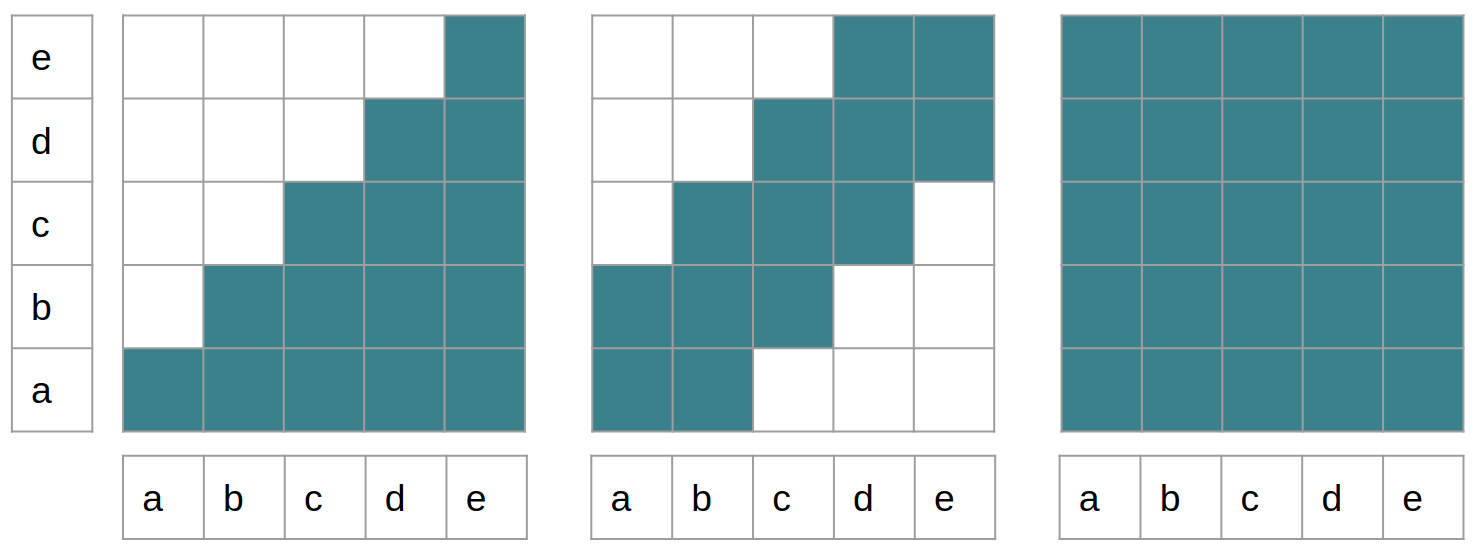
\includegraphics[width=\textwidth]{graphics/encoding.png}
\caption[Illustration of context range at each token in different encoding mechanism]{Illustration of context range at each token in different encoding mechanism. From left to right: Recurrent encoder, Convolutional encoder, Attention-based encoder. The example sequence is $[a,b,c,d,e]$ and each colored column represent the context range of the corresponding token.}
\label{fig:encoding}
\end{figure*}

The decoder works similarly to a language model as it predicts one token per time step. However, the decoder conditions its prediction on the source sequence. Therefore, the decoder takes the output of the encoder as its inputs. An Auto-regressive decoder conditions its prediction on the predictions of previous steps and the source sequence. Because all of our experiments use auto-regressive NMT, from now, a decoder is an auto-regressive decoder if there is no other specification. The decoder usually uses the same neural architecture as the encoder. However, unlike the encoder, the range of context of a token is strictly limited to its preceding tokens. Because the hidden state of the decoder is computed from the previous hidden states and the observation of the previous step, we need to initialize the $0^{th}$ hidden state $s_0$ (optional) and the $0^{th}$ token. That is why we always begin the target sequence by the token $<BOS>$, and the decoder starts predicting from the second token. For example, if $[a,b,c,d,e]$ is predicted by the decoder, the prediction of token $a$ is conditioned by source sequence $x$ and $<BOS>$; the prediction of token $b$ is conditioned by source sequence $x$ and $[<BOS>,a]$ and so on. Besides, the decoder needs a signal to stop its generative prediction. We always end a prediction by "end-of-sentence" token or $<EOS>$. Therefore, instead of predicting $[a,b,c,d,e]$, the decoder predicts $[a,b,c,d,e, <EOS>]$. Concerning the construction of hidden states, the Recurrent decoder usually initializes $s_0$ by the last hidden state of the encoder followed by a linear transformation. In contrast, the Convolutional decoder and the Attention-based decoder do not need to initialize $s_0$ as every hidden state directly accesses the predictions preceding its time step without going through its preceding state. We illustrate the difference between decoding paradigms in the figure \ref{fig:decoding}.

\begin{figure*}[htbp]
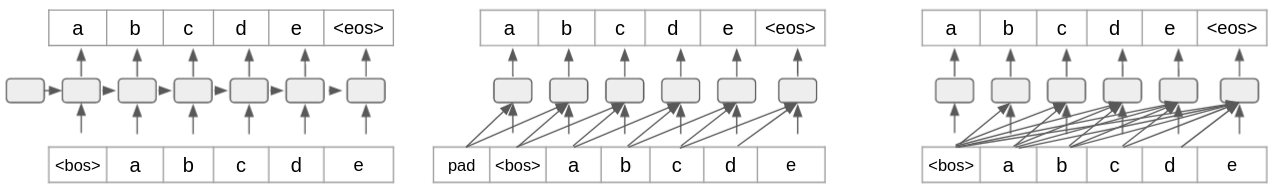
\includegraphics[width=\textwidth]{graphics/decoding.png}
\caption[Illustration of 3 most popular auto-regressive decoding paradigms]{From left to right: Recurrent decoder, Convolutional decoder, Attention-based decoder. The example sequence is $[a,b,c,d,e]$. The figure illustrates only one layer of the decoder.}
\label{fig:decoding}
\end{figure*}

NMT's Encoder/Decoder is usually a stack of multiple layers. As described above, the input source sequence is mapped to a sequence of word embeddings. This is considered as $0^{th}$ layer of the Encoder. The $i^{th}$ layer is built upon the $(i-1)^{th}$ layer by applying the same encoding mechanism, which can be recurrent layer, convolutional layer or self-attention layer, to the output of the $(i-1)^{th}$. We illustrate different multi-layer decoders in figure \ref{fig:multi-layer}. For example, \citet{Vaswani17attention} stacked 6 Transformer layers in both the encoder and the decoder of the NMT model. Deep NMT models are able to learn from very large-scale of parallel data \citep{Ott18scaling} and continually create new state-of-the-art performances. However, deep NMT models are harder to train because the gradient flow has to back-propagate through many layers. In order to prevent the gradient flow from vanishing, which happens when the value of the output of the linear transformation in some layer jumps outside the domain of the activation function, \citep{He16deep} proposes using residual connections, which replaces $f(x)$ by $f(x)+x$ where $x$ is the output of the lower layer and $f(.)$ is the transformation of the layer, to transit from the lower layers to their following layers. By using residual connections, a fraction of the gradient still reaches the lower layer and continues to propagate until the lowest layer.

Deep NMT models also suffer from Internal Covariate Shift in which the distribution of the value of each layer significantly changes due to the change of the parameters of the models. In deep network, the distribution of the value of high layers is highly affected by the parameters of the lower layers and can be dramatically shifted by a small change in the value of those parameters. Large shift can push the value of the layer to the saturation zone of activation function where the gradient is extremely small. In practice, the saturation problem can be mitigated by using the Rectified Linear Units $RELU(x) = max(x,0)$ \citep{Nair10rectified}. Recently, \citep{Ioffe15batch,Jimmy16layer} propose different normalization methods to stabilize the value of layers so that they are not easily pushed to saturation zone of activation function. In principle, Normalization methods re-scale and re-center the distribution of the value of each layer with learnable mean and learnable variance. Normalization methods prove to be very helpful in practice. For example, Layer normalization must be included in every layer of Attention-based NMT \citep{Vaswani17attention}.

\begin{figure*}[htbp]
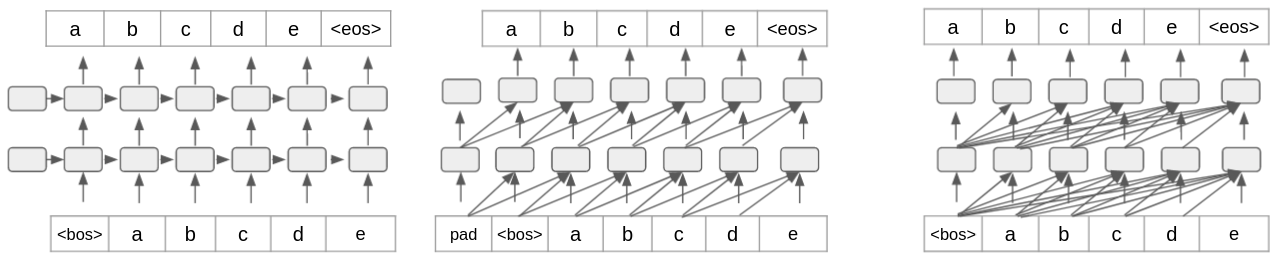
\includegraphics[width=\textwidth]{graphics/multi_layer_decoder.png}
\caption[Illustration of 3 most popular multi-layer auto-regressive decoding paradigms]{From left to right: Recurrent decoder, Convolutional decoder, Attention-based decoder. The example sequence is $[a,b,c,d,e]$. The figure illustrates only two layers of the decoder.}
\label{fig:multi-layer}
\end{figure*}

\section{Recurrent neural machine translation} \label{sec:rrn}
\nomenclature[rnn]{RNN}{Recurrent neural network}
This section reviews the very first NMT architecture, the Recurrent neural machine translation (RNMT\nomenclature[rnmt]{RNMT}{Recurrent neural machine translation}). RNMT is composed of a Recurrent encoder, a Recurrent decoder, and tables of word embeddings. Recurrent encoder and Recurrent decoder usually use the same type of Recurrent neural network (RNN) layer, such as Gated recurrent unit (GRU) and Long-short term memory (LSTM), which we will explain in the following section. RNMT is strictly auto-regressive as each hidden state in the encoder/decoder has to go through every intermediate state to assess the information of any time step before it. The hidden states of RNMT inherit the information of the order, which is an advantage before Convolutional neural machine translation (CNMT\nomenclature[cnmt]{CNMT}{Convolutional neural machine translation}) and Attention-based neural machine translation (ANMT\nomenclature[anmt]{ANMT}{Attention-based neural machine translation}), from this encoding paradigm. However, a lack of straightforward access to positions of the input sequence causes many difficulties in the training of RNMT.

\subsection{GRU, LSTM layers}
\nomenclature[gru]{GRU}{Gated recurrent unit}
\nomenclature[lstm]{LSTM}{Long-short term memory}
Gated recurrent unit (GRU) and Long-short term memory (LSTM) are the two most popular layers in the group of Recurrent neural network. They follow the auto-regressive paradigm by constructing the hidden states one by one as follows
\begin{equation}
\begin{array}{rcl}
h^l_t = f(h^{l-1}_t, h^l_{t-1})
\end{array}
\end{equation}
where $h^{l-1}_t$ is the hidden state at time step $t$ of the $(l-1)^{th}$, the $0^{th}$ layer is the sequence of word embeddings; the mapping f can be GRU cell or LSTM cell, which will be explained below.

LSTM was first introduced by \citet{Hochreiter97long}. It uses 4 gating functions including input gate i, output gate o, forget gate f and memory cell c. At each time step t, the contextualized embedding $h_t$ is computed as follows
\begin{equation}
\label{eq:lstm}
\begin{array}{rcl}
f_t &=& \sigma_g (W_f h^{l-1}_t + U_f h_{t-1} + b_f),\\
i_t &=& \sigma_g (W_i h^{l-1}_t + U_i h_{t-1} + b_i),\\
o_t &=& \sigma_g (W_o h^{l-1}_t + U_o h_{t-1} + b_o),\\
\tilde{c}_t &=& \sigma_c (W_o h^{l-1}_t + U_o h_{t-1} + b_o),\\
c_t &=& f_t \odot c_{t-1} + i_t \odot \tilde{c}_t,\\
h_t &=& o_t \odot \sigma_h(c_t),\\
\end{array}
\end{equation}
where $\sigma_g$ is the sigmoid function, $\sigma_c$ is the hyperbolic tangent function, $\sigma_h$ is either the hyperbolic tangent function or the identity function and $\odot$ is the element-wise multiplication. These functions are applied element-wise to intermediate vectors in the equations.

The motivation behind this highly complex structure is to stabilize the exploding/diminishing gradient flow \citep{Pascanu13onthe} conducted by back-propagation through time (BPTT \nomenclature[bptt]{BPTT}{Back-propagation through time}) \citep{Hochreiter97long}. The second architecture GRU, which was proposed by \citet{Cho14properties}, mitigates the complexity of LSTM by using only three gates as follows.
\begin{equation}
\label{eq:gru}
\begin{array}{rcl}
z_t &=& \sigma_g (W_z h^{l-1}_t + U_z h_{t-1} + b_z)\\
r_t &=& \sigma_g (W_r h^{l-1}_t + U_r h_{t-1} + b_r)\\
\hat{h}_t &=& \sigma_h (W_h h^{l-1}_t + U_h (r_t \odot h_{t-1}) + b_h)\\
h_t &=& (1-z_t)\odot h_{t-1} + z_t \odot \hat{h}_t\\
\end{array}
\end{equation}
Where $\sigma_h$ is a hyperbolic tangent function while other notations are the same as in the equations \ref{eq:lstm}.
\subsection{RNN encoder}
RNN encoder uses LSTM or GRU layer to encode the source sequence. RNN encoder can use more than one layer to capture more fine-grained language representation \citep{Li20shallow}. The $0^{th}$ layer is a sequence of word embeddings, which are extracted from the look-up table of the source side using the indices provided by the source sequence. 

\subsubsection{Bidirectional RNN encoder}
Unlike the decoder, the encoder is not obliged to process the input sequence from left to right. Effectively, the context of one token in the source sequence contains not only its preceding neighbors but also its following neighbors. Therefore, encoding the source sequence from left to right is not enough to cover the context of each token. To increase the coverage of contextualized embedding, the encoder process the source sequence both from left to right and from right to left at the same time therefore the encoder becomes a bidirectional encoder. Bidirectional encoding results in two sequences of contextualized embeddings; the encoder simply combines two contextualized embeddings of a token into one real vector via either concatenation or summation. The resulting contextualized embedding captures information of every word in the source sequence around its corresponding token. 
\subsection{RNN decoder}
RNN decoder predicts the target sequence from left to right, one token per time step. It initializes the $0^{th}$ hidden state by zero vector or a linear transformation of the last hidden state of the last layer of the encoder. The following section will discuss on an import component of the NMT model, which attention mechanism. As the hidden representation of the decoder at each step is computed as follow
\begin{equation}
s_i = g(s_{i-1},y_{i-1},c_i),
\end{equation}
where $c_i$ is context vector. $c_i$ is computed via attentional mechanism using $s_i$ and $Enc(x)$, which will be explained in Section \ref{ssec:attention}.

The prediction probability will be computed as follow
\begin{equation}
p(y_i|s_i,y_{i-1},c_i) = softmax(Dense(t_i))_{y_i}
\end{equation}
where $y_i$ is an index of the target vocabulary, $Dense$ is a dense layer, whose output is of dimension $|\Sigma_y|$, and $t_i$ is compute as follow
\begin{equation}
\begin{array}{rcl}
t_i &=& \big[ max\big\{ \tilde{t_{i,2j-1}}, \tilde{t_{i,2j}} \big\} \big]^{T}_{j=1,\cdots,d}, \\
\tilde{t}_i &=& U_0 s_{i-1} + V_0Emb(y_{i_1}) + C_0c_i,
\end{array}
\end{equation}
where $Emb(y_{i-1})$ is the word embedding of the token $y_{i-1}$, $U_0 \in \mathbb{R}^{2l\times d}$, $V_0 \in \mathbb{R}^{2l\times d'}$, and $C_0 \in \mathbb{R}^{2l\times d}$ in case uni-directional encoder and $C_0 \in \mathbb{R}^{2l\times 2d}$ in case bi-directional encoder.
\subsubsection{Attentional mechanism \label{ssec:attention}}
An attentional mechanism consists of 3 components: Query vectors, Key vectors, and Value vectors. Given a sequence $Q_i$, $i \in [1 \cdots n]$, $K_j$, $j \in [1 \cdots m]$ and $V_j$, $j \in [1 \cdots m]$, the results
of the attentional mechanism composed by those vectors will be as follow
\begin{equation}
Attention(Q,V,K)_i = \displaystyle{\mathop{\sum}_{j=1}^{m}} \frac{exp(sim(Q_i,K_j))}{\displaystyle{\mathop{\sum}_{p=1}^{m}}exp(sim(Q_i,K_p))}*V_j, i \in [1, \cdots, m],
\end{equation}
where the function $sim(x,y)$ can be the standard dot product $<x,y>$ \citep{Vaswani17attention}, a generalized dot product $<x,W_a*y>$ or $<v_a, tanh(W_a*[x,y])>$ \citep{Luong15stanford, Bahdanau15learning}.

The attentional mechanism manages and quantifies the dependence between the input sequence and the output sequence (e.g., source contextualized embeddings and target contextualized embeddings), or the input sequence itself (e.g., self-attention layers in Transformer \citep{Vaswani17attention}). In the RNN MT model, the attentional mechanism is used to capture the dependence of each token in the target sequence on the tokens in the source sequence. For example, \citet{Bahdanau15learning} computed a context vector at $i^{th}$ time step in the decoder as follows
\begin{equation}
\begin{array}{rcl}
c_i &=& \sum_{j} \alpha_{ij} h_j, \\
\alpha_{ij} &=& \frac{exp(e_{ij})}{\sum_{k}exp(e_{ik})}, \\
e_{ik} &=& sim(s_{i-1},h_k),\\
\end{array}
\end{equation}
where $h_j$ is the output of the last layer of the encoder, $s_{i-1}$ is the hidden state at the $(i-1)^{th}$ time step of the last layer of the decoder. 

%This context vector will be used to compute the hidden state at $i^{th}$ position by the attentional mechanism improves the translation quality of very long sequences. Indeed, the context vector produced by the RNN encoder struggles to capture all the dependence between tokens of the input sequence because it lacks the direct links between 2 tokens. The information of a token vanishes while the encoder moves toward the far ending of the input sequence. The same problem happens with the decoder when it decodes the context vector into the output sequence. The attentional mechanism provides the direct links from each output token to any input token, allows the decoder to capture the information of any input token regardless of its position.

\section{Convolutional neural machine translation} \label{sec:cnn}
\nomenclature[cnn]{CNN}{Convolutional neural network}
The convolutional neural network was successfully applied to the MT task in the work of \citet{Ghering17convolutional} that outperformed the current state-of-the-art performance of the RNMT. As we mentioned in the previous section, Convolutional neural machine translation (CNMT) does not construct the hidden states iteratively in one direction. The model considers the sequence as an image, of which each column of pixels is a word embedding, and applies convolutional kernels on it. Therefore, the CNMT is much faster than the RNMT. We give the detail of the Convolutional encoder and Convolutional decoder in the following sections.
\subsection{Convolutional encoder}
Concretely, each layer of Convolutional encoder contains a one dimensional convolution kernel followed by a non-linear activation function. We denote $h^l_i$ the $i^{th}$ hidden state of the $l^{th}$ layer. Those hidden states are computed as follows
\begin{equation}
\begin{array}{lcr}
h^l_i = v\bigg( W^l \big[h^{l-1}_{i-\frac{k}{2}}, \cdots, h^{l-1}_{i+\frac{k}{2}} \big] + b_w \bigg) + h^{l-1}_{i},
\end{array}
\end{equation}
where $W^l \in \mathbb{R}^{2d \times kd}$, $b_w \in \mathbb{R}^{2d}$, d is the dimension of hidden states as well of word embeddings, k is the width of the kernel, the activation function v is Gated Linear Unit \citep{Ghering17convolutional} as follows
\begin{equation}
\begin{array}{lcr}
v([A,B]) = A \odot \sigma(B),
\end{array}
\end{equation}
where $\odot$ is element-wise multiplication, $\sigma$ is sigmoid function.
\subsection{Convolutional decoder}
Unlikely the Convolutional encoder, in which each hidden states has access to its left and right neighbors, the decoder only allows left accesses to avoid conditioning the predictions on the following tokens, which remain unknown before the prediction during the inference. Therefore, \citet{Ghering17convolutional} appended $k-1$ padding tokens in the left side of the output sequence, e.g $PAD$, $PAD$,$ <BOS>$,$je$,$t'$,$aime$ for convolution kernel of size 3 so that $\big[ PAD, PAD, <BOS>\big]$ predicts $je$, $\big[ PAD,<BOS>,je\big]$ predicts $t'$ and so forth.
The Convolutional decoder also uses an attention mechanism to improve the performance of long sentences. \citet{Ghering17convolutional} proposed a version slightly different from ones of \citet{Luong15stanford, Bahdanau15learning}. For each $l^{th}$ decoder layer, the query will be a combination of the hidden state $h^l_i$ and the word embedding of the previous token $g_i$ as follows
\begin{equation}
\begin{array}{rcl}
Q^l_i = W^l_d h^l_i + b^l_d + g_i.
\end{array}
\end{equation}
The keys are still the hidden states of the last layer of the encoder $z^u_j$. The values are the combinations of the hidden states $z^u_j$ and the word embedding $e_j$ as follows
\begin{equation}
\begin{array}{rcl}
V^l_j = z^u_j + e_j.
\end{array}
\end{equation}
The score attention is the dot product between the query vector and the key vector followed by the softmax function as follows
\begin{equation}
\begin{array}{rcl}
\alpha_{ij}=\frac{exp(Q^l_i \cdot z^u_j)}{\sum_{t=1}^m exp(Q^l_i \cdot z^u_t)}.
\end{array}
\end{equation}
The context vector $c^l_i$ will be as follow
\begin{equation}
c^l_i = \sum_{j=1}\alpha_{ij}V^l_j
\end{equation}
Once $c^l_i$ has been computed, it is simply added to the output of the corresponding decoder layer $h^l_i$.
\subsection{Positional embedding}
\citet{Ghering17convolutional} proposed using embeddings corresponding to each position of the input sequence. The purpose is to equip the CNMT model with a sense of order as the Convolution kernel does not take into account the order of tokens in the input sequence. Effectively, if we interchange the position of tokens outside the window of the kernel, the value of the hidden state does not change. Positional embeddings are real value vectors having the same dimension as word embeddings. Positional embeddings are added to word embeddings of the corresponding position before passing to the first layer.

\section{Attention-based neural machine translation} \label{sec:transformer}
Transformer architecture was first introduced by \citet{Vaswani17attention} and has quickly become the state-of-the-art architecture not only in MT but also in language modeling (LM)  \citep{Devlin19bert,Brown20language,Conneau19cross}, text summarization \citep{Zhang20pegasus} etc. The Transformer model's power relies on the attentional mechanism, which was discussed in the previous section \ref{ssec:attention}. The Transformer model consists of a fully attention-based encoder and decoder. 
\subsection{Transformer encoder}
\label{ssec:transformer-enc}
The Transformer encoder consists of layers made of a multi-head self-attention sub-layer followed by a position-wise fully connected feed-forward network. The multi-head self-attention sub-layer is an extension of the self-attention sub-layer and is described by the following equation
\begin{equation}
\begin{array}{rcl}
MultiheadAttention\big( Q,V,K \big) &=& Concat \big[ head_0, \cdots , head_h \big] W_0\\
head_i &=& Attention \big( QW_i^Q, VW_i^V, KW_i^K \big),\\
\end{array}
\end{equation}
where $W_i^Q, W_i^V, W_i^K \in \mathbb{R}^{d_k \times d_h}$ with $d_h \times h = d_k$, $d_k$ is the dimension of word embedding space and also the size of Transformer model. Unlike the version \eqref{eq:self-att} in Section \ref{ssec:attention}, the attentional mechanism is simply as follows,
\begin{equation}
Attention\big( Q, V, K \big) = Softmax\big(\frac{Q K^T}{\sqrt{d_k}} \big) V.
\end{equation}
The feed-forward network is designed as follows
\begin{equation}
FFN(x) = ReLu(xW_1+b_1)W_2+b_2,
\end{equation}
where $W_1 \in \mathbb{R}^{d_k \times d_b}$,$W_2 \in \mathbb{R}^{d_b \times d_k}$,$b_1 \in \mathbb{R}^{d_b}$,$b_2 \in \mathbb{R}^{d_k}$.
The final detail is that the output of each sub-layer has to pass through a Layer-Normalization sub-layer \citep{Jimmy16layer}. In conclusion, the contextualized embedding of the $l^{th}$ layer of the Transformer encoder will be as follows
\begin{equation}
\begin{array}{rcl}
\tilde{h}^l &=& LN\bigg(Multihead\big(h^{l-1}, h^{l-1}, h^{l-1}\big) + h^{l-1}\bigg), \\ 
h^l &=& LN\bigg(FFN\big(\tilde{h}\big) + \tilde{h}\bigg),
\end{array}
\label{eq:self-att}
\end{equation}
where $LN$ is a Layer-Normalization sub-layer.
\subsection{Transformer decoder}
The Transformer decoder consists of layers made of a multi-head self-attention sub-layer followed by a multi-head cross-attention sub-layer then by a position-wise fully connected feed-forward network. The multi-head self-attention sub-layer and the feed-forward network have the same design as those in the Transformer encoder. The multi-head cross-attention sub-layer of the $l^{th}$ layer of the decoder uses the output of the last layer of the encoder as keys and values, the output of the $l^th$ self-attention sub-layer as queries
\begin{equation}
\begin{array}{rcl}
\tilde{s}^l &=& LN\bigg( Multihead\big( s^{l-1},s^{l-1},s^{l-1} \big) + s^{l-1} \bigg), \\
\bar{s}^l &=& LN\bigg( Multihead\big( \tilde{s}^l, h^u, h^u \big) + \tilde{s}^l \bigg), \\
s^l &=& LN\bigg( FFN\big( \bar{s}^l \big) + \bar{s}^l \bigg), \\
\end{array}
\end{equation}
where $s^l$,$s^{l-1}$ are the outputs of the $l^{th}$ and $(l-1)^{th}$ layers of the decoder respectively, $h^u$ is the output of the last layer of the encoder.

In order to prevent the future information in the decoder, at each time step $i^{th}$, the attention scores of tokens at positions after $i^{th}$ are masked by zero.

\subsection{Positional embedding}
Similar to the Convolutional encoder/decoder, the Transformer encoder/decoder does not respect the order of tokens as it fully connects every pair of tokens in parallel. In order to represent the position of tokens in the sequence, \citet{Vaswani17attention} proposed the use of positional embedding. Unlike \citet{Ghering17convolutional}'s positional embedding, this version is not parameterized as given the size of word embedding $d_k$ , the positional embedding of position $i^{th}$ is defined as 
\begin{equation}
\begin{array}{rcl}
PE\big(pos,2i\big) &=& sin \big( \frac{pos}{1000^{\frac{2i}{d_k}}} \big)\\
PE\big(pos,2i+1\big) &=& cos \big( \frac{pos}{1000^{\frac{2i}{d_k}}} \big).\\
\end{array}
\end{equation}
The positional embedding will be added to the corresponding word embedding of the $i^{th}$ token of the input sequence.
\section{Training NMT models} \label{sec:train}
The purpose of training NMT model is to find optimal values for its parameters so that the error of the model are minimal in the testing. To learn these optimal values, we need 3 type data sets including training set, validation set, and testing set. Training set is used to optimize the model's parameters via statistical learning algorithms such as Maximum likelihood estimation (MLE\nomenclature[mle]{MLE}{Maximum likelihood estimation})\citep{Baum87Supervised}. Testing set is used to evaluate the model once it's optimized. The performance on the testing set shows us how good the model is and is used to compare different models. Validation set is not used to learn the model's parameters nor to evaluate the model but to prevent the "over-fitting" of the optimization. Effectively, an NMT model can be trained until very small error in the training set but has poorer performance in the testing set than another NMT model which is trained with early stopping criteria. During the training, the model is evaluated on the validation set for every $K$ iterations. The learning is represented by 2 learning curves, including the error on training set and the error on the validation set. The stopping criteria is whether the validation error does not improve after a predetermined number of consecutive evaluations.

Concerning the optimization of the model on the training set, we usually use MLE, i.e.
\begin{equation}
\hat{\theta} = \displaystyle{\mathop{argmax}\mathop{\sum}_{x,y \in \mathit{D}}}log P(y|x;\theta),
\label{eq:mle}
\end{equation}
where $\mathit{D}$ is the sampling distribution of the training data.
MLE is equivalent to minimizing the cross-entropy loss
\begin{equation}
\begin{array}{rcl}
L_{CE}(\theta,\mathit{D}) &=& -\displaystyle{\mathop{\sum}_{(x,y) \in \mathit{D}} \mathop{\sum}_{i}^{l_y}}log P(y_i|y_{<i},x;\theta), \\
\hat{\theta} &=& \displaystyle{\mathop{argmax}} L_{CE}(\theta).
\end{array}
\end{equation}
In order to optimize this function, we often use the gradient descent method, which is one of the oldest approaches in the Optimization area \citep{Cauchy1847method}. The gradient is computed by back-propagation algorithm \citep{Rumelhart88learning}. Like many deep learning models, the NMT model is usually trained with a massive amount of data that makes the gradient descent method is not computationally plausible. Therefore, stochastic gradient descent (SGD\nomenclature[sgd]{SGD}{Stochastic gradient descent}) is proposed to mitigate the computational burden of large-scale models \citep{Herbert51stochastic,Kiefer52stochastic,Bottou10large}. Instead of calculating the gradient of the loss over every training examples, SGD samples a batch of examples from training set, calculates the gradient of the loss over this batch, then updates the parameters according to this gradient.
\subsection{Tips and tricks in training an NMT model}
Deep Neural networks are usually very hard to train. Effectively, back-propagation through time in RNMT usually creates exploding or vanishing gradients \citep{Pascanu13onthe,Glorot10understanding}. Gradient clipping \citep{Pascanu13onthe}, Truncate back-propagation \citep{Jaeger02tutorial} are proposed to mitigate this problem.

Large NMT models are easily over-fitted to training data. \citet{Srivastava14Dropout} proposed randomly freezing a subset of parameters during one training iteration, which prevents the whole model from being fitted to one example. We could interpret Dropout as an ensemble method that allows training many sub-networks in one training and ensembles them in testing. In practice, Dropout is essential to train neural models in general. 

Besides, the Log-likelihood maximizing \eqref{eq:mle} assumes that a ground-truth label is far more likely than all other labels, excessively discriminates between the likelihood of training examples and the likelihood of language that does not appear during training. The Log-likelihood maximizing can result in over-fitting to the training data, reducing the model's generalization in testing.

\section{Inference with an NMT model} \label{sec:inference}
An NMT model translates a source sentence $x$ by searching the target sequence y that gives the highest probability conditioned on $x$,
\begin{equation}
\hat{y} = \displaystyle{\mathop{\argmax}}. P(y|x;\theta)
\end{equation}
However, the search space of $y$ is of infinite dimension, causing the implausibility of the exact search. Beam search \citep{Och98improving} is the most common inference algorithm in Neural Machine Translation and Statistical Machine Translation. For autoregressive NMT models, a single output token is produced at each inference step $j$. The prediction at step $j$ is conditioned by $x$ and the partial translation hypothesis up to step $j$
\begin{equation}
\hat{y}_j = \displaystyle{\mathop{\argmax}_{y_j \in \Sigma_y}} P(y_j|y_{<i},x,\theta).
\end{equation}
Beam search tracks K most probable translation hypothesis. Beam search starts with K empty hypotheses, which are initialized by "begin of sentence" token $<BOS>$. In the $j^{th}$ inference step,
for the $n^{th}$ partial hypothesis $[y^{n}_{<j}]$, the top-K most probable tokens according to $P(.| y_{<j},x;\theta)$ are picked and appended to the current hypothesis
\begin{equation}
\hat{y}^n_j \in \displaystyle{\mathop{Top_{K}}_{y_j \in \Sigma_y}} P(y_j|y_{<j},x,\theta).
\end{equation}
The search space, therefore, is extended to $K*K$ hypotheses. Beam search selects only the top $K$ hypotheses from these $K*K$ hypotheses. It stops extending an hypothesis when $<EOS>$ is predicted or  the hypothesis reaches the predefined length limit. 

Beside the left-to-right decoding, there are several variant decoding direction including non-monotonic decoding \citep{Welleck19non}, non auto-regressive decoding \citep{Jiatao17non}, and synchronous bidirectional decoding \citep{Zhou19synchronous}. Because the decoding algorithms are not included in this research topic, we would like to be limited to this brief description.
\nomenclature[eos]{EOS}{end-of-sentence}
\section{MT evaluation}
The evaluation of MT systems can be done automatically by comparing n-grams of generated translations and n-grams of gold references. The most popular MT metric is BLEU \citep{Papineni02bleu}. Recently, \citet{Post18A} proposed standardizing hypotheses of MT systems before calculating BLEU metric. 

BLEU is computed on corpus-level, i.e., it compares a corpus of hypotheses and the corpus of references. BLEU score is the geometry average of n-gram precisions, including 1-gram, 2-grams, 3-grams and 4-grams weighted by brevity penalty (BP)
\begin{equation}
BLEU = BP exp(\frac{1}{4}\sum_{i=1}^4log p_i).
\end{equation}

The n-gram precision $p_n$ is computed as follows
\begin{equation}
p_n = \frac{\sum_{hyp \in hyps}\sum_{n\text{-}gram \in n\text{-}grams} min(Count(Ref,n\text{-}gram), Count(hyp, n\text{-}gram))}{\sum_{hyp \in hyps}\sum_{n\text{-}gram \in n\text{-}grams} Count(Ref,n\text{-}gram)},
\end{equation}
Where $Count(C,g)$ is the number of occurrences of the n-gram $g$ in the corpus $C$.

The Brevity penalty computed as follows
\begin{equation}
  BP =
    \begin{cases}
      1 & \text{if $|c| > |r|$ }\\
      exp(1-\frac{|r|}{|c|}) & \text{otherwise}.
    \end{cases}       
\end{equation}
Where $c$ is the total length of the hypothesis corpus, $r$ is the total length of the reference corpus. The Brevity penalty assures that a high-scoring candidate translation must also match the reference translations in length.








































	\chapter{Machine translation (multi-)domain adaptation's review} \label{chap:revisting}
Machine translation (multi-)domain adaptation has a long history as the area has been actively studied for almost two decades and is still being explored to communicate many languages in many fields better. The earliest domain adaptation methods were explored for SMT systems. Recently, most of the effort has been made to adapt better NMT systems to domains for NMT has surpassed SMT to be state-of-the-art architecture. In this chapter, we would like to do our best to give a thorough literature review of the problem. More precisely, we formally point out 4 principle cases of (multi-)domain adaptation and revise the approaches for each case. We also adopt the survey of \cite{Chu18asurvey} in our review.

We divide this chapter into five sections. In the first section \ref{sec:domain}, we would like to discuss how we usually define a domain, how translations differ between domains and the importance of domain adaptation in real applications. In the second section \ref{sec:multi-facet} we would like to regroup two notions, domain adaptation, and multi-domain adaptation, then divide the large problem MT (multi-)domain adaptation into four sub-problems. We dedicate four following sections to those sub-problems. In each of the four following sections, we review groups of approaches, according to \citet{Chu18survey}, that match the requirement of the corresponding problem.
\section{What is a domain?}
\label{sec:domain}
In a classical machine learning context such as binary classification problem, \citet{Shai10A} defined a domain by a pair consisting of a distribution $\mathcal{D}_x$ on inputs $\mathcal{X}$ and a labeling function $f: \mathcal{X} \rightarrow [0,1]$. In machine translation context, the labeling function will be $f: \mathcal{X} \rightarrow \mathcal{Y}$ where $\mathcal{X}$ and $\mathcal{Y}$ are the set of sentences of the source language and the target language respectively. Denote 2 different domains, $\big( \mathcal{D}_S, \mathcal{F}_S \big)$ and $\big( \mathcal{D}_T, \mathcal{F}_T \big)$. Domain adaptation is required when we train a machine learning model (statistical or neural) with data generated by $\big(\mathcal{D}_S, \mathcal{F}_S \big)$ but test it with data generated by $\big(\mathcal{D}_S, \mathcal{F}_S \big)$. In principle, there is no guaranty that the model performs well in the second domain. However, we could aim to exploit some sharing knowledge between the two domains; for example, \citet{Blitzer06Domain} explored pivot features, which are features that frequently occur in the two domains and similarly contribute to the predictions in both domains. The context of machine translation is much more complicated than binary classification as the label is a structured sequence of symbols that has to satisfy both the adequacy according to the source sequence and the fluency according to the target language. \cite{Wees15Whats,Wees17Whats} identified the following elements of text, which influence the translation the most.
\begin{itemize}
	\item Topic: the subject of the text such as medical, news, IT, or religious. A topic owns its own specific vocabulary, terminologies. These items can not be transferred between distant topics such as medical and religion.
	\item Genre: the purpose of the text such as education, talk, report, or instruction. It identifies groups of texts that share a common form of transmission, purpose, and discourse properties. We characterize genre by textual style, the structure of the text, etc.
\end{itemize}

Despite many specifications, domains share the same grammar of the corresponding language. However, the concepts such as the grammar, the textual style, or the text structure are abstract to machine translation models. MT models learn to translate from examples without being explicitly explained how to do it. They are supposed to learn this knowledge to translate, but we cannot tell whether they do it until now.

Solving the MT (multi-)domain adaptation problem is essential for deploying MT in a real context. Machine Translation has applications in many sectors, such as translating legal documents, news, scientific documents, books, movie subtitles, etc. Every domain has its own specific vocabulary, registers(formal or informal), and genres (e.g., talk, instruction). Therefore, tailoring MT models to a target domain is essential to achieve good translation in that domain. In practice, MT models (SMT, NMT) trained with domain-related data always perform much better in the domain of interest than ones trained with the same amount of less relevant data \citep{Rico13domain, Saunders21Domain}. The more domain-relevant data is available, the better the MT system performs in the target domain. However, not every domain has enough data to train an MT model. The state-of-the-art architecture ANMT will need millions of parallel sentence pairs to learn its parameters. Therefore, we have to work around the situation where there is very little data or even no data. Domain Adaptation aims to improve the performance of an MT model in low-resourced domains. Besides, multi-domain adaptation seeks to achieve the best performance in more than one domain. However, the domains of interest in multi-domain adaptation are not limited to be low-resourced domains. The motivation of having one model adapted to many domains is to optimize the storage, the training time, and the deploying time. Having one model per domain increases the storage, the time retrieving a model, and thus the translation latency. Online translation services, such as Google Translate, Systran Translate, or DL Translate, have to translate text from any possible domain while minimizing the latency of translation in order to be beneficial. In conclusion, the variety of text between fields requires domain adaptation, while fast and robust translation requires multi-domain adaptation.

\section{Machine translation (multi-)domain adaptation a multi-faceted problem}
\label{sec:multi-facet}
\subsection{From domain adaptation MT to multi-domain adaptation MT}
Even though domain adaptation and multi-domain adaptation do not have same motivation as one focuses on low-resourced domain whereas the other focuses on adapting to as many as possible domains, they can be cast under one general framework. Formally, training instances are distributed according to a mixture $\mathcal{D_S}$ such that $\mathcal{D_S}(x) = \sum_{d=1}^{n_d} \lambda^{s}(d) \mathcal{D}_d(x)$, with $\{\lambda^{s}(d), d=1 \dots n_d\}$ the mixture weights satisfying $\sum_d \lambda^{s}(d)=1$. The target domains are represented in the test distribution which is also a mixture of $\mathcal{D_T}(x) = \sum_{d=1}^{n_d} \lambda^{t}(d) \mathcal{D}_d(x)$, with $\{\lambda^{t}(d), d=1 \dots n_d\}$ the mixture weights satisfying $\sum_d \lambda^{t}(d)=1$. We assume $\mathcal{D}_d(x), d=1 \dots n_d\}$ is the support of the both source and target distribution. Domain adaptation solves the case where $\lambda^s * \lambda^t = 0$ and $\lambda^t$ is one-hot vector while multi-domain adaptation happens to solve the case where $\lambda^t$ is not one-hot vector. We illustrate this formulation in figure %\ref{fig:mdmt-lambdas}.
\begin{figure}[h]
  \centering
  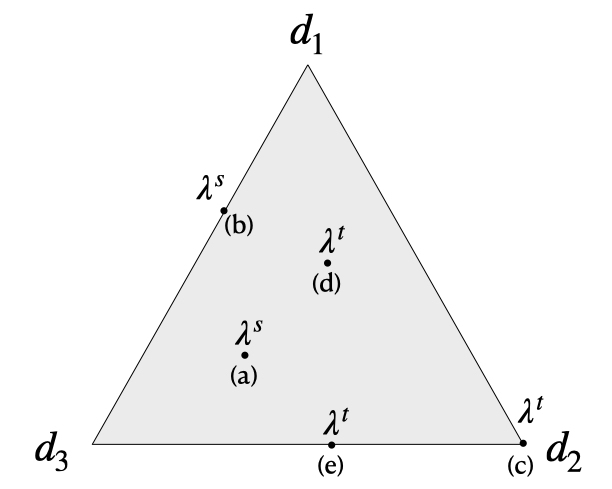
\includegraphics[width=0.5\textwidth]{graphics/mdmt-lambdas}
  \caption[Training and testing with distribution mismatch]{Training and testing with distribution mismatch. We consider just three domains, and represent vectors of mixture weights $\vlambda^{s}$ and $\vlambda^{t}$ in the 3-dimensional simplex. Training with weights in (a) and testing with weights in (c) is supervised multi-source domain adaptation to domain~2 ($d_2$), while (b)-(c) is the unsupervised version, with no training data from $d_2$; training with weights in (a) and testing with weights in (d) is multi-domain learning, also illustrated with configurations (a)-(e) (training domain $d_1$ is not seen in test), and (b)-(d)  (test domain $d_2$ is unseen in training).}
  \label{fig:mdmt-lambdas}
\end{figure}

This framework modelizes the real context closely because, in a typical setting in machine translation, we collect the most extensive collection of parallel data for the chosen language pair to achieve optimal performance for the task of interest. In such situations, the training data distribution is opportunistic. The test data distribution is determined and fixed; a key component in training is to mitigate the detrimental effects of a possible mismatch between these distributions. Training data may be a mixture of many domains such as the JRC-Acquis Communautaire corpus (\domain{law}-domain) \citep{Steinberger06acquis} or documentation for KDE, Ubuntu, GNOME and PHP from the Opus collection \citep{Tiedemann09news} (\domain{it}-domain). We also leverage a collection of data with no specific topic and genre, such as Paracrawl \citep{Banon20Paracrawl}. The testing data represent the domains of interest. In multi-domain adaptation, because there are multiple target domains, the testing is composed of multiple tests. The performance of an MT system is usually the average of its performance on these tests. However, we can access the quality of the multi-domain MT system with different priorities over target domains using weighted mean. The evaluation of multi-domain MT system should be clarified before training as early stopping criteria relies on the evaluation over validation tests.
\subsection{4 main sub-problems}
From our study on many previous works, we realize that the (multi-)domain adaptation problem is a multifaceted problem. Effectively, all the cases of (Multi-)domain adaptation can be classified into four groups by answering two following questions:
\begin{itemize}
	\item Is/Are the domain(s) of the training deterministic?
	\item Is/Are the domain(s) of the testing deterministic?
\end{itemize}
More precisely, the first question asks whether the training data is composed of a number of known domains. For example, the domain of a mixture of multiple corpora of specific topics, such as JRC-Acquis Communautaire corpus (\domain{law}-domain) and KDE (\domain{it}-domain), is well defined. However, the domains in Paracrawl \citep{Banon20Paracrawl} is unknown because it was built by crawling the content of web-sites without specifying topic or purpose. The second question asks whether the domain of the testing data is determined. If there exists a collection of text (monolingual or parallel) that defines the domain of the testing, then it is domain-deterministic and vice versa. 

Our first case of (multi-)domain adaptation \ref{sec:case1} is supervised multi-domain adaptation in which domain labels are both available in training and testing. Furthermore, the target domains in testing are included in the training. This case might be the most straightforward situation. Many approaches in multi-domain MT conducted their experiments in this setting \cite{Pham21revisiting}. 

The second case \ref{sec:case2} considers the use of the parallel data crudely collected from webs such as Paracrawl \citep{Banon20Paracrawl} or Commoncrawl \footnote{\url{https://commoncrawl.org/}}. The content of these corpora varies from many topics, but unfortunately, there is not any available domain label for sentences. Fortunately, in the second case, the target domains are known, i.e., there exist data of these domains, which can be used to adapt the model. The second case focuses on the exploitation of opportunistic text. 

The third case \ref{sec:case3} assumes a well domain-labeled training data while allowing the testing sentence from any possible domain. This case focuses on the robustness of the MT system against any possible shift distribution in testing. The third setting is very closed to real applications where the provenance of the input text is unknown. 

Finally, the last setting \ref{sec:case4} focuses on both exploiting opportunistic data in training and being robust against unknown testing distribution. We dedicate the four following sections to discuss more details of each setting.

Recently the work of \citet{Chu18survey} significantly captured the landscape of MT domain adaptation by categorizing previous methods in 2 main classes: data-centric and model-centric. The data-centric category includes methods that manipulate the training distribution to resemble the distribution of the target domain better. The model-centric methods focus on changing the architecture, modifying the training objective, and improving the inference.

According to \citet{Chu18asurvey}, the data-centric focuses on two paradigms, including 1) collecting parallel data related to the domain target, 2) creating synthetic data resembling the domain target. The first paradigm searches for similar examples to the ones of the domain target to enlarge the domain target's training data. The second paradigm aims to create pseudo examples resembling the data of the domain target. Besides the two paradigms, we propose another paradigm, which is data sampling. The data sampling paradigm consists of changing the data sampling distribution during the training course to mitigate the heterogeneity of the data size between domains and the variety of the "difficulty" of the domains. Therefore data-centric consists of 3 paradigms, including 1) data collection, 2) data synthesization, and 3) data sampling.

This taxonomy is largely adopted in MT domain adaptation's research. However, we find a naivety in this classification as it misses delivering an answer for the most ultimate question: "which method solves which problem?". We propose adding another dimension, the context of the MT adaptation problem, to form a Cartesian map of the MT (multi-)domain adaptation area. The four following sections will explain how model-centric and data-centric categories solve 4 (multi-)domain adaptation cases. We believe that this coupling of methods and cases will allow us to navigate better the (multi-)domain adaptation forest that has been growing for almost two decades. We also introduce several unexplored adaptation problems that need more research effort and other applications of existing application methods. The work of \citet{Pham21revisiting} recently gave a brief review of several well-known adaptation methods via a reevaluation with different domain adaptation cases. However, the experiments are still limited in the first case \ref{sec:case1} and the third case \ref{sec:case3} by excluding crawled corpora.

\section{Supervised (multi-)domain adaptation}
\label{sec:case1}
In the supervised (multi-)domain adaptation, the domain label is available in both training and testing. Furthermore, the domain(s) in testing is(are) available in training. In this problem, we would like to achieve a unique model that performs the best in one or many target domains, given training data from those domains and probably from other domains. This setting is the most popular situation on which multi-domain machine translation research papers focus. The first case represents the least requirement as the MT needs to achieve the best performance on the domains it learned from. The difficulty of this situation is to both exploit the proximity between domains while mitigating the interference due to inter-domain heterogeneity. Effectively, similar topics, such as legal and administrative, might improve the vocabulary coverage of each other as both domains share the same specific terminologies. However, distant topics, such as religion and IT might confuse the MT system when sharing the same parameters. In the following sections, we will discover how model-centric methods and data-centric methods solve this case.
\subsection{Model-centric}
In the case of the supervised multi-domain adaptation, model-centric methods focus on adding domain-specified parameters to reduce the interference between domains while keeping the number of parameters small. The simplest methods use domain tags. For example, \citet{Kobus17domain} proposed appending a special token to each source sequence indicating its domain such as $<Domain=IT>$ and train the NMT model with this format. However, this format requires domain tags in testing; hence we have to predict them if the source sentences are from an unknown origin. \cite{Britz17effective} originally proposed appending domain tag to the target sequence so that the decoder will predict the domain in which it will generate the translation. Instead of using domain tag, \citep{Kobus17domain, Pham19generic} proposed using domain embedding to incorporate the domain information into the context of the translation. \citet{Kobus17domain} concatenated an embedding of small size (e.g., 4) to the embedding of each token in the input sequence. Each small embedding corresponds to a domain. Instead of using the same domain embedding for the tokens in the same domain \citet{Pham19generic} used lexicalized domain representation, which is a small embedding correspond to the domain and the token. Besides domain embedding, we can use domain-specified layers that can be plugged between 2 consecutive layers of the NMT model without changing the architecture. There are 2 types of plug-in layers: 1) residual adapter \citep{Bapna19simple, Pham20Study} and 2) learning hidden unit contribution \citep{Vilar18learning}. Residual adapters were first introduced by \citet{Rebuffi17learning} in computer vision. \citet{Bapna19simple} proposed this fine-tuning paradigm for domain adaptation. They introduced a new version of residual adapter composed of 2 linear projections and the ReLU activation function. The adapters are plugged into the NMT model as follow
\begin{equation}
\begin{array}{rcl}
h_{enc/dec}^l = h_{enc/dec}^{l} + ADAP_{enc/dec}^l(h_{enc/dec}^{l})
\end{array}
\end{equation}
where $ADAP_{enc/dec}^l$ is the adapter corresponding to the $l^{th}$ layer of the encoder/the decoder. \cite{Pham20Study} studied the use of the residual adapters for multi-domain adaptation and propose several techniques, including regularization, gating mechanism, to improve the robustness of the model. The learning hidden unit contribution (LHUC \nomenclature[lhuc]{LHUC}{Learning hidden unit contribution}) method was proposed by \cite{Vilar18learning} to adapt an NMT model to a domain. The author applied an LHUC layer to the model as follow
\begin{equation}
h_{enc/dec}^l = h_{enc/dec}^{l} \odot a(\rho^{l}_{enc/dec})
\end{equation}
where $\rho^{l}_{enc/dec}$ is the adapter corresponding to the $l^{th}$ layer of the encoder/the decoder and $\rho^{l}_{enc/dec} \in \mathbb{R}^d$. $a(.)$ is a scaled
element-wise sigmoid function.
$$a(x) = \frac{2}{1+e^{-x}}$$
Residual adapter and learning hidden unit contribution layer adapt a pretrained model without changing its parameters. 

While the previous methods aim to discriminate domains to reduce the interference,\cite{Britz17effective} was motivated to learn hidden representations that are invariant between domains. More precisely, the authors use a binary classifier that takes the output of the encoder as input to distinguish the source sequences of 2 source domains. They inverse the sign of the gradient corresponding to the loss of the classifier to confuse it, i.e., making the hidden representation of the encoder invariant between 2 domains. This technique is related to A-distance, which is a measure of similarity between two probability distributions. \cite{Ben07analysis} showed that the A-distance between the
source and target distributions is a crucial part of an upper generalization bound for domain adaptation. They hypothesized that it should be difficult to discriminate between the source and target domains to have a good transfer between them because
this would imply similar feature distributions. \cite{Zeng18multidomain}'s work was also inspired by this idea. However, instead of forcing the encoder's output to be invariant between domains, the authors focus on extracting domain-agnostic features and domain-specific features from the output of the encoder and feeding the features to the decoder. To do that, they use two different non-linear transformations, which map a hidden representation to two vectors of the same size. Then, they apply one domain classifier on each extracted feature vector. The domain-agnostic feature vector is trained to confuse its corresponding classifier, whereas the domain-specific feature vector is trained to facilitate its classifier.

\cite{Michel18extreme} adapted a pretrained model to a multi-user personalized model by fine-tuning the
bias of the output softmax to each particular user of the MT system. The number of additional parameters is $|S| \times |\Sigma_y|$, in which $S$ is the set of the users. The author reduces the size of the bias matrix $B \in \mathbb{R}^{|S| \times |\Sigma_y|}$, whose each row is a bias vector of one user, by factoring it into lower dimension representation, i.e.
\begin{equation}
\begin{array}{rcl}
B &=& S \times \tilde{B}, \\
&where& \\
S & \in & \mathbb{R}^{|S| \times r}, \\
\tilde{B} & \in & \mathbb{R}^{r \times |\Sigma_y|}.
\end{array}
\end{equation}

\citet{Jiang20Multi}'s work was inspired by the mixture of expert paradigm. Their novel model is based on Transformer architecture \citep{Vaswani17attention} as they integrate a domain-mixing mechanism to the multi-head attention layer. As we explained in Section ~\ref{ssec:transformer-enc}, each head of multi-head attention layer is computed as follow
\begin{equation}
head_i = Attention \big(QW_i^Q, VW_i^V, KW_i^K \big).
\end{equation}
Suppose that there are $K$ domains, at the $i^th$ head, for each query, key and value component, there are $K$ transformation matrix $W_{i,j}^Q | j \in [1,K]$, $W_{i,j}^K | j \in [1,K]$, $W_{i,j}^V | j \in [1,K]$ respectively. The domain-mixing mechanism is applied on query, key and value components as follow
\begin{equation}
\begin{array}{rcl}
Q_i^t &=& \sum_{j=1}^K Q^tW_{i,j}^Q*\mathit{D}_j(x_t),\\
K_i^t &=& \sum_{j=1}^K K^tW_{i,j}^K*\mathit{D}_j(x_t),\\
V_i^t &=& \sum_{j=1}^K V^tW_{i,j}^V*\mathit{D}_j(x_t),\\
head_i &=& Attention \big( Q_i, K_i, V_i\big),
\end{array}
\end{equation}
where the subscript $t$ indicates the position of the vector in the sequence of hidden representations, $\mathit{D}(x_t) \in \mathbb{R}^{K}$ is the domain proportion of the corresponding token $x_t$. The proportion of domains of a token is computed by a domain classifier, that take the input embedding of that token as input. The novel model adapt the hidden representation of a token to a domain to which the token likely belongs. Therefore, the model is able to discriminate domains in domain-specific tokens while transfering knowledge between domains in domain-agnostic tokens. However, the size of the model is proportional to the number of domains, which is not practical in the real applications. However, in our opinion, the idea can be applied to lightweight adapter or learning hidden unit contribution layer.

Besides the model-centric methods related to the architecture, multi-task training is another solution to the supervised (multi-)domain adaptation problem. 

We illustrate several well-known model-centric methods for the supervised domain adaptation problem in Figure~\ref{fig:model-centric-case1-case2}.
\begin{figure}[htbp]
\begin{subfigure}{1.0\textwidth}
  \centering
  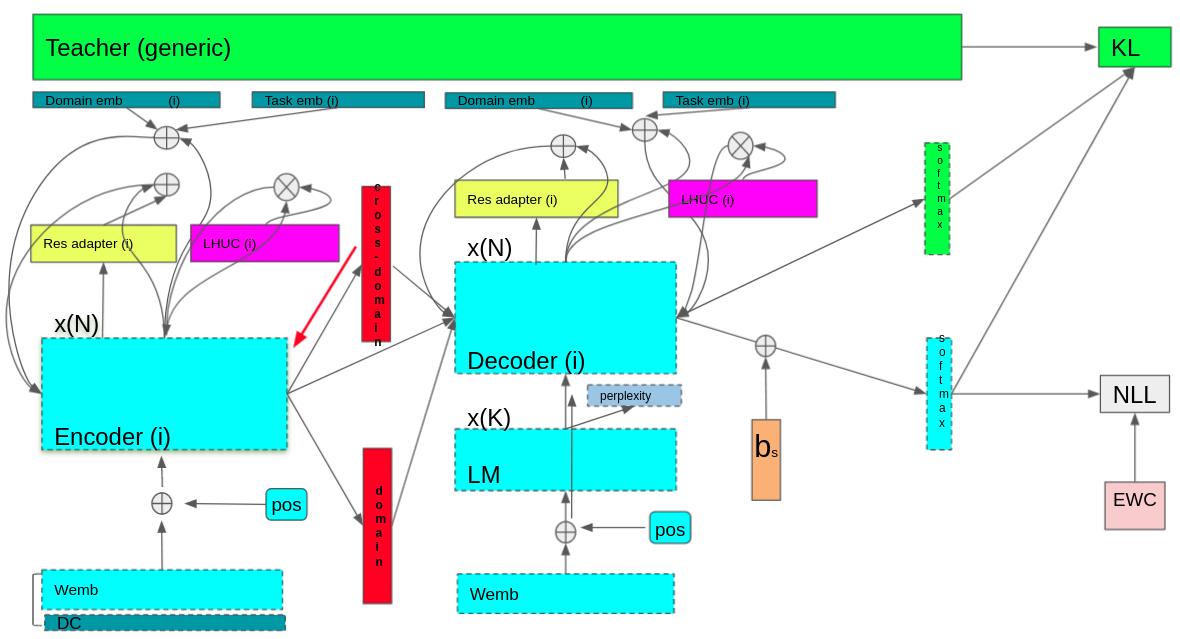
\includegraphics[width=1.0\textwidth]{graphics/supervised_mdmt}
\end{subfigure}
\newline
\begin{subfigure}{1.0\textwidth}
  \centering
  \fbox{\begin{tabular}{ll}
\textcolor{red}{$\blacksquare$} & \citep{Zeng18multidomain} \\
\textcolor{violet}{$\blacksquare$} & \citep{Vilar18learning} \\
\end{tabular}}
\end{subfigure}
\caption[Model-centric's brief overview]{Each color different from the bleu corresponds to one model-centric method. The bleu represents the NMT model.}
\label{fig:model-centric-case1-case2}
\end{figure}

\subsection{Data-centric}
\subsubsection{Data sampling}
In supervised multi-domain adaptation, data sampling approaches aim to balance the contribution of each domain to the final model. In an opportunistic multi-domain training data, the data size of each domain vary from few thousands examples to millions examples. In a trivial mixture of data, small domains are usually excessively under-sampled causing a sub-optimal performance in average. However, if we equally sample data from every domain, the NMT model is easily over-fitted in the small domains. Therefore, finding optimal sampling distribution of domains is essential. \cite{Wang20balancing} proposed parameterizing the probability of sampling data from a domain and learned this probability via REINFORCE algorithm \citet{Williams92simple} using rewards computed from cosine-similarity between the gradient over in-domain training data and the gradient over dev-sets' data. We compare this technique to our approach in chapter \fyTodo{add reference of chapter MDAC here}.

Other data-centric methods, that does not take into account the domains of the training data will be discussed in Section ~\ref{ssec:case-2-data}.
\section{Non domain-deterministic training, domain-deterministic testing}
\label{sec:case2}
In this situation, the training data is composed by a number of unknown domains. The second case focuses on adapting the NMT model with an unknown source domain while the target domain is well defined. There are two situations: 1) there exists parallel data in the target domain 2) there exists only monolingual data in the target domain. The two following sections will discuss how each group of method solve these cases.
\subsection{Model-centric}
First, we discuss the case with one target domain in which there exist parallel data. In this case, we can apply the same techniques proposed for supervised (multi-)domain adaptation by considering the source domain as a generic domain. Besides, fine-tuning is very efficient approach for this problem\citep{Luong15stanford,Miceli17regularization,Servan16Domain,Freitag16fast}. We first train an NMT model with the mixture of source domains, then continue training this model with the parallel data of the target domain. According to a recent review of multi-domain adaptation conducted by \citet{Pham20Priming}, fine-tuning is the strongest baseline in supervised domain adaptation. However, fine-tuned NMT models usually suffer from catastrophic forgetting \citep{Michael89catastrophic} as their performances drop dramatically in the source domains. To mitigate the catastrophic forgetting, several regularization techniques were introduced, including mixed fine-tuning \citep{Chu17empirical}, uniform weight-decay \citep{Miceli17regularization}, elastic weight consolidation (EWC \nomenclature[ewc]{EWC}{Elastic weight consolidation}) \citep{Brian19overcoming, Kirk16overcoming, Saunders19domain} and knowledge distillation \citep{Dakwle17fine}. 

Mixed fine-tuning \citep{Chu17empirical} adapts an NMT model with the mixture of the source domain and the target domain (by oversampling the target domain). The method adapts the NMT model to the domain of interest thanks to the oversampling while maintaining its robustness to generic text as it is trained with the source domain.

Weight decay \citep{Miceli17regularization} continues the training on the target domain's data with a regularized loss 
\begin{equation}
L_{CE}(\theta,\mathit{D}_{target}) + \alpha * \parallel \theta - \theta^{A} \parallel_{L_2},
\end{equation}
where $\theta^{A}$ is the value of the pretrained model. Fine-tuning with the new loss fits the model to the target domain while preserving the parameters' old pretrained values, therefore preventing the overfitting of the NMT model in the target domain and maintaining the generality over source domains. \citet{Brian19overcoming, Kirk16overcoming, Saunders19domain} were also motivated to penalize the changes of the parameters compared to the old model. However, the authors argued that not every parameter has the same contribution to maintain the generality to the old domains and that we can tune the parameters unimportant to the old domains to the target domain. The contribution of each parameter of the pretrained model is approximated by the diagonal of the Fisher matrix computed over the data of the source domains. Therefore, fine-tuning with EWC uses the following loss
\begin{equation}
L_{CE}(\theta,\mathit{D}_{target}) + \sum_{i} \frac{\lambda}{2} F_i * (\theta_i - \theta_i^{A})^2,
\end{equation}
where the $F_i$ is the $i^th$ element of the diagonal of the Fischer matrix approximated as follow
\begin{equation}
\bar{F} = \frac{1}{|\mathit{D}_{source}|} \displaystyle{\mathop{\sum}_{(x,y)\in \mathit{D}_{source}}} \nabla log(p(y|x,\theta))_{| \theta^{A}} \nabla log(p(y|x,\theta))_{| \theta^{A}}^{T}
\end{equation}
\citet{Dakwle17fine}'s method was motivated by knowledge distillation paradigm \citep{Hinton15Distilling}. The authors propose regularizing the standard cross-entropy loss with the Kullback-Leibner distance \citep{Kullback51On} between two predicting distributions produced by old model and new model as follow
\begin{equation}
L_{CE}(\theta,\mathit{D}_{target}) + \alpha * \displaystyle{\mathop{\sum}_{(x,y)\in \mathit{D}_{source}}} KL(p(.|x,\theta) | p(.|x,\theta_{A})).
\end{equation}

Instead of continuing the training with target domain only, \citet{Chen17cost} differentiated directly domain-relevant instances and irrelevant instances via instance weighting. The authors compute the weight of each instance by a domain classifier, that is trained with source sequences. The training will maximize the following objective 
\begin{equation}
\begin{array}{rcl}
\hat{\theta} = \displaystyle{\mathop{\arg max}_{\theta} \mathop{\sum}_{(x,y)\in D_{in} \cap D_{out}}} (1+p_d(x))log(P(y|x,\theta))
\end{array}
\end{equation}
where $D_{in}$, $D_{out}$ are the target domain and other domains, $p_d(x)$ is the probability that $x$ comes from the target domain. \citet{Wang17instance} proposed using different domain-relevance metric for instance weighting. 

Besides the auxiliary losses, ensemble methods are also promising. For example, \citet{Freitag16fast} proposed ensembling the pretrained model and the fine-tuned model to combine the advantage of both models: the specialization in the target domain and the generalization over general text.

Still in the case of the uni-domain adaptation, but without parallel data. The model-centric approaches mostly use monolingual data in the target language of the target domain. The proposed methods mostly adapted the decoder to the target domain. For example, \citet{Gulcehre16monolingual} proposed training a language model adapted to the target domain and fusing the language model to the decoder. The fusion could be deep or shallow. The deep fusion combined the hidden representation of the decoder and the one of the language model before computing the prediction probability. The shallow fusion combined the prediction probability computed by the decoder and the one computed by the language model. \citet{Domhan17using} was also motivated by this idea. However, the authors proposed jointly training the language model and the NMT model via multi-task training. Furthermore, the decoder and the language model shared the word embedding of the target side.

All previous methods were motivated to adapt an NMT model to a specific domain. We realize that they can hardly be applied to multi-domain adaptation because all the parameters of the MT model are adapted to one domain. However, in the case where there are parallel data of the target domains, we could use model-centric methods proposed in the supervised adaptation by considering the training domain a generic domain. Recently, \cite{Dou19unsupervised} proposed using domain-embedding and task-embedding to adapt an NMT model to the target domain using reconstruction loss on the monolingual data. More precisely, for each layer $l^{th}$ of an ANMT model, there are 2 task embeddings $\theta_{task}^{\gamma,l}$, $\gamma \in \{ MT, LM \}$, which correspond to translation task and language modeling task respectively. Furthermore, for each layer $l^{th}$, and for each domain $d$, there is a domain task $\theta^{d,l}_{dom}$. The layer $l^{th}$ of encoder/decoder will be as follow
\begin{equation}
h^{l} = LAYER^l(h^{l_1}) + \theta^{d,l}_{domain} + \theta_{task}^{\gamma,l}
\end{equation}
Now, the parallel data will be used to compute translation loss, while the monolingual data is used to compute language modeling loss. The authors proposed adding noises to the source sequence while computing the LM loss. Using domain-specific embeddings enables the model to be adapted to multiple domains at once. Despite being applied to multi-lingual machine translation, the monolingual adapter proposed by \citet{Philip20monolingual} shares the same spirit and can be applied to this situation.
\subsection{Data-centric}
\label{ssec:case-2-data}
According to our study, the previous data-centric approaches proposed to this situation belong to all three paradigms, including data selection, data synthesization, and data sampling. The two following sections will discuss the methods of each paradigm.
\subsubsection{Data selection}
Data selection approaches collect parallel data, which resemble the target domain. The selection is usually based on a score of proximity between a parallel example and the domain. The score of proximity can be computed via sentence embedding or variants of \citeauthor{Moore10intelligent} score. For example, given two corpora of a target domain $D_{I-src}$, $D_{I-tgt}$ and two corpora of the source domain $D_{O-src}$, $D_{0-tgt}$, \cite{Axelrod11domain} computed a bilingual version of Moore $\&$ Lewis score of a sentence pair as follow
\begin{equation}
\begin{array}{rcl}
S_{bi} (x,y) &=& H_{I-src}(x) - H_{O-src}(x) + H_{I-tgt}(y) - H_{O-tgt}(y), \\
\end{array}
\label{eq:ced}
\end{equation}
where the cross-entropy $H_{*}(z)_{| * \in [I-src, I-tgt, O-src, O-tgt], z \in [x,y]}$ of the sentence $z$ is computed by a language model trained only with the corpus $D_{*}$. \citet{Duh13adaptation} proposed the same formulation as proposed \citet{Axelrod11domain} but used a neural language model instead of a statistic language model. In a survey of data selection methods for neural machine translation, \citet{Silva18extracting} evaluated 3 popular methods in the domain adaptation task, including cross-entropy difference, Term Frequency-Inverse Document Frequency (TF-IDF \nomenclature[tf-idf]{TF-IDF}{Term Frequency-Inverse Document Frequency}) \citep{Salton73On} and Feature Decay Algorithm (FDA) \citep{Poncelas18Feature}. More precisely, cross-entropy difference was performed as described above and normalized by sentence length. To perform TF-IDF, \citet{Silva18extracting} consider each sentence of the target domain as a query and every sentence in the source domain as a key. The tf-idf vectors of the queries and the keys are computed as in \citet{Salton73On}. The score of proximity between a query and a key is the cosine-similarity of theirs tf-idf vectors. Based on the score of proximity, for each sentence of the target domain, we retrieve K nearest-neighbors in the source domain. The collection of the retrieved sentences is the result of the method. The last method FDA extracts from the source domain a set of sentences that better represent a given test set provided by the source side of the target domain. \revision{The detail of the algorithm is referred to the work of \citet{Poncelas18Feature}.}

\cite{Wang17sentence} proposed using sentence embedding to represent a sentence instead of a tf-idf vector. For each language side (source/target) the authors computed the centroid of the target domain and one of the source domain. Assume $C_{E_{in}}$, $C_{E_{out}}$ are the centroid of the target domain and the source domain in the source language,  $C_{F_{in}}$, $C_{F_{out}}$ are the centroid of the target domain and the source domain in the source language, $v_{\mathit{e}}$ is the sentence embedding of a source sentence $\mathit{e}$, $v_{\mathit{f}}$ is the sentence embedding of a source sentence $\mathit{f}$, then the proximity of the example $(\mathit{e},\mathit{f})$ to the target domains is defined as follow
\begin{equation}
d(v_{\mathit{e}}, C_{E_{in}}) - d(v_{\mathit{e}}, C_{E_{out}}) + d(v_{\mathit{f}}, C_{F_{in}}) - d(v_{\mathit{f}}, C_{F_{out}}),
\end{equation} 
where $d(.,.)$ is the Euclidean distance in $\mathbb{R}^d$. \cite{Aharoni20unsupervised} proposed using sentence embedding computed by a pretrained Bidirectional Encoding Representation Transformer (BERT \nomenclature[bert]{BERT}{Bidirectional Encoding Representation Transformer}) and the cosine-similarity to retrieve domain-related examples.

\subsubsection{Data synthesization}
The most efficient approach of this paradigm is backtranslation \citep{Sennrich16improving}, which consists of translating the monolingual data of the target language to the source language. \citet{Burlot18using} showed significant improvement of an NMT model in the target domain when trained with the mixture of parallel data and the in-domain backtranslated data. Without backtranslating the target-side data, \citet{Currey17copied} created artificial sentence pairs from the monolingual data in the target language so that each source sentence is identical to the target sentence. Training an NMT model with the mixture of parallel data and artificial sentences improves the accuracy of the translation on named entities and other words that should remain identical between the source and target languages. 

\subsubsection{Data sampling}
Data sampling methods dynamically change the composition of the training data over time. A difference between data sampling and data selection is that data sampling does not keep the same training data after the collection. However, the two paradigms are orthogonal. In practice, the evolution of the training data is beneficial for training an NMT model specialized to a domain. For example, fine-tuning is similar to this paradigm as the training begins with every available data and finishes with the data of the target domain. However, data sampling methods consist of building an automatic curriculum without human supervision. For example, \citet{Wees17dynamic} proposed gradual fine-tuning, which first computes a sampling distribution based on the cross-entropy difference (CED) \eqref{eq:ced} of each example, then gradually decreases the number of examples sampled from previous distribution for each epoch. Formally, the CED score of each example is normalized as follow
\begin{equation}
\tilde{CED}(x) = 1 - \frac{CED(x)-min(CED_{G})}{max(CED_{G}) - min(CED_{G})},
\end{equation}
where $G$ is the training corpus. Therefore the higher-ranked example has a higher $\tilde{CED}$ score rather than having lower $CED$ as in \cite{Axelrod11domain}. The sampling distribution is computed as follow
\begin{equation}
\omega(x) = \frac{\tilde{CED}(x)}{\sum_{x'\in G} \tilde{CED}(x')}.
\end{equation}
For each epoch $i^{th}$, a number $n_i$ of examples are selected according to the previous distribution. $n_i$ is defined as follow
\begin{equation}
n_i = \alpha \cdot |G| \cdot \beta^{\lfloor \frac{i-1}{n}, \rfloor}
\end{equation}
where $\alpha \in [0,1]$ is the relative start size, $\beta \in [0,1]$ is the retention rate. Via the same mechanism, \citet{Wang19dynamically} proposed a more sophisticated dynamical sampling distributions combining two scores of an example, including domain-CED and noise-CED. The authors proposed two variants, including mixed co-curriculum, which score an example by the sum of its CED scores, and cascaded co-curriculum, which first selects examples by domain-CED then retains top examples according to noise-CED from previous selection. Furthermore, \citet{Wang19dynamically} proposed to recompute the language model of noisy data for each epoch. Instead of increasing the domain-relevance of the training data, \cite{Zhang19curriculum} did the opposite. More precisely, they reordered the training data according to their relevance to the target domain then equally split the whole corpus into many shards containing samples of a similar score. They trained an NMT model with one shard per epoch in decreasing order of domain-relevance.

Besides well-known metrics for domain-relevance, \citet{Zhang19curriculum} proposed a parameterized scorer, that evaluates the usefulness of each sample to the performance on the target domain, and optimized its parameters via Bayesian optimization. More precisely, the scorer was formulated as follow
\begin{equation}
\mathit{f}(x,y) = V \cdot \mathbf{F}(x,y),
\end{equation}
where feature vector $\mathbf{F}(x,y)$ was extracted from the example, and weight vector $V$ was learned by Bayesian optimization. Each element of $\mathbf{F}(x,y)$ represented the relevance of the example to a target domain. Once the scorer was optimized, the training was conducted similarly as in \citet{Wees17dynamic,Wang19dynamically}.

\section{Domain-deterministic training, non domain-deterministic testing}
\label{sec:case3}
The third case is interesting because it resembles the real context of machine translation's applications. Effectively, the users' text can be from any possible topic or for any possible purpose (genre). In this situation, the NMT model needs to be both robust to the unseen domains and adapted to the known domains. 
\subsection{Model-centric}
Mixture model is effective to this situation as it combines domain-adapted systems to perform the translation. Effectively, the performance of mixture model is guaranteed in the source domains while using a convex combination of the adapted systems is robust against the unseen domains. Mixture model has been successfully applied for SMT models \citep{Sennrich12perplexity, Carpuat14linear, Sennrich12mixture}. \citet{Sajjad17neural, Saunders19domain,Freitag16fast} applied mixture model to NMT models. The contribution of each adapted model to the combination was uniform in \citet{Freitag16fast} while \cite{Sajjad17neural} pre-finetuned them by bayesian optimization on a development set. However, heuristic static weight is sub-optimal when the testing domain is highly variable. \citet{Saunders19domain} proposed computing the weights of the mixture for each source sentence $x$ at $i^{th}$ decoding step as follow
\begin{equation}
\begin{array}{rcl}
W_{k,i} &=& \displaystyle{\mathop{\sum}_{t} P(t|h_i,x)\lambda_{k,t}}, \\
&where& \\
P(t|h_i,x) = P(t|x) &=& \frac{\displaystyle{P^k_{LM}(x)}}{\displaystyle{\mathop{\sum}_{k'} P^{k'}_{LM}(x)}},\\
\end{array}
\end{equation}
where $P^{k'}_{LM}(x)$ is the probability of the source sentence $x$ according to the language model learned from domain $k'$, $\lambda_{k,t}$ can be uniform, identity or pre-finetuned with a development set. \citet{Saunders19domain} also proposed varying the mixture's weights during the inference by conditioning the domain posterior probability on both $x$ and $h_i$ as follow
\begin{equation}
P(t|h_i,x) = \frac{P(h_i|t,x) P(t|x)}{\displaystyle{\mathop{\sum}_{k'} P(h_i|k',x) P(k'|x)}}.
\end{equation} 
However, one might be more interested in domain robustness than domain specialization. The mixture model does not include the domain robustness in the training objective. \cite{Muller20domain} discussed several regularization methods to mitigate the problem, including subword regularization \citep{Taku18subword}, defensive distillation \citep{Papernot16distillation}, reconstruction \cite{Tu17neural} and neural noisy channel reranking \citep{Li16mutual}. Distributional robustness \citep{Oren19distributionally,BenTal13robust} is also a promising paradigm as the methods optimized learning models so that they perform well over a wide range of potential test distributions. However, the application of this paradigm to neural machine translation is not yet discovered.
\subsection{Data-centric} \label{ssec:data-centric}
Data-centric can not be applied to this situation as non domain-deterministic testing does not provide the domain of the test sentences. Effectively, data-centric requires the monolingual data of the target domain to create the pseudo in-domain data while the testing domain is non deterministic.
\section{Non domain-deterministic training, non domain-deterministic testing}
\label{sec:case4}
\subsection{Model-centric}
\cite{Li18onesentence, Farajian17multidomain} proposed finetuning on-the-fly the pretrained model to a mini-batch similar to the source sentence before translating it. The authors chose the learning rate and the number of finetuning iterations according to the score of similarity between the mini-batch and the source sentence so that the higher similarity the higher the learning rate, the more iterations. \cite{Pham20Priming,xu20boosting,Bulte19neural} proposed learning NMT model to reuse memory translations whose source sentence is similar to the source sentence. 
\subsection{Data-centric}
The data-centric paradigm can not be applied to this situation for the same reason as the previous section \ref{ssec:data-centric}















































































































































































































































































































































































	\chapter{Revisiting multi-domain machine translation}
  When building machine translation systems, one often needs to make the best out of heterogeneous sets of parallel data in training, and to robustly handle inputs from unexpected domains in testing. This multi-domain scenario has attracted a lot of recent work, that fall under the general umbrella of transfer learning.
In this study, we revisit multi-domain machine translation, with the aim to formulate the motivations for developing such systems and the associated expectations with respect to performance. Our experiments with a large sample of multi-domain systems show that most of these expectations are hardly met and suggest that further work is needed to better analyze the current behaviour of multi-domain systems and to make them fully hold their promises.

\section{Introduction} \label{sec:intro}

Data-based Machine Translation (MT), whether statistical or neural, rests on well understood machine learning principles. Given a training sample of matched source-target sentence pairs $(\src,\trg)$ drawn from an underlying distribution $\mathcal{D}_s$, a model parameterized by $\theta$ (here, a translation function $h_{\theta}$) is trained by minimizing the empirical expectation of a loss function $\ell(h_\theta(\src), \trg)$. This approach ensures that the translation loss remains low when translating more sentences drawn from the same distribution.

Owing to the great variability of language data, this ideal situation is rarely met in practice, warranting the study of an alternative scenario, where the test distribution $\mathcal{D}_t$ differs from $\mathcal{D}_s$. In this setting, \emph{domain adaptation} (DA) methods are in order. DA has a long history in Machine Learning in general (e.g.\ \cite{Shimodaira00improving,Ben10A,Quinonero08dataset,Pan10asurvey}) and in NLP in particular (eg.\ \cite{Daume06domain,Blitzer07domain,Jiang07instance}). Various techniques thus exist to handle both the situations where a (small) training sample drawn from $\mathcal{D}_t$ is available in training, or where only samples of source-side (or target-side) sentences are available (see \cite{Foster07mixture,Bertoldi09domain,Axelrod11domain} for proposals from the statistical MT era, or \cite{Chu18asurvey} for a recent survey of DA for Neural MT).

A seemingly related problem is \emph{multi-domain} (MD) machine translation \cite{Sajjad17neural,Farajian17multidomain,Kobus17domain,Zeng18multidomain,Pham19generic} where one single system is trained and tested with data from multiple domains. MD machine translation (MDMT) corresponds to a very common situation, where all available data, no matter its origin, is used to train a robust system that performs well for any kind of new input.
If the intuitions behind MDMT are quite simple, the exact specifications of MDMT systems are rarely spelled out: for instance, should MDMT perform well when the test data is distributed like the training data, when it is equally distributed across domains or when the test distribution is unknown? Should MDMT also be robust to new domains? How should it handle domain labeling errors? 

A related question concerns the relationship between supervised domain adaptation and multi-domain translation. The latter task seems more challenging \revision{as it tries to optimize MT performance for a more diverse set of potential inputs, with an additional uncertainty regarding the distribution of test data.} Are there still situations where MD systems can surpass single domain adaptation, as is sometimes expected?   

In this paper, we formulate in a more precise fashion the requirements that an effective MDMT system should meet (Section~\ref{sec:requirements}). Our first contribution is thus of methodological nature and consists of lists of expected properties of MDMT systems and associated measurements to evaluate them (Section~\ref{sec:challenging}). In doing so, we also shed light on new problems that arise in this context, regarding for instance the accommodation of new domains in the course of training, or the computation of automatic domain tags. Our second main contribution is experimental and consists in a thorough reanalysis of eight recent multi-domain approaches from the literature, including a variant of a model initially introduced for DA. We show in Section~\ref{sec:experiments} that existing approaches still fall short to match many of these requirements, notably with respect to the handling of a large amount of heterogeneous domains and to dynamically integrating new domains in training.
 
\section{Requirements of multi-domain MT \label{sec:requirements}}
In this section, we recap the main reasons for considering a multi-domain scenario and discuss their implications in terms of performance evaluation.

\subsection{Formalizing multi-domain translation \label{ssec:formalization}}

We conventionally define a domain $d$ as a distribution $\mathcal{D}_d(x)$ over some feature space $\mathcal{X}$ that is shared across domains \cite{Pan10asurvey}: in machine translation, $\mathcal{X}$ is the representation space for source sentences; each domain corresponds to a specific source of data, and differs from the other data sources in terms of textual genre, thematic content \cite{Chen16guided,Zhang16topicinformed}, register \cite{Sennrich16politeness}, style \cite{Niu18multitask}, etc. Translation in domain $d$ is formalized by a translation function $h_d(y|x)$ pairing sentences in a source language with sentences in a target language $y \in \mathcal{Y}$. $h_d$ is usually assumed to be deterministic (hence $y = h_d(x)$), but can differ from one domain to the other.

A typical learning scenario in MT is to have access to samples from $n_d$ domains, which means that the training distribution $\mathcal{D}^s$ is a mixture $\mathcal{D}^s(x) = \sum_d \lambda^{s}_{d} \mathcal{D}_d(x)$\revision{, with $\{\lambda^{s}_d, d=1 \dots n_d\}$ the corresponding mixture weights ($\sum_d \lambda^{s}_d=1$)}. Multi-domain learning, as defined in \citet{Dredze08online} further assumes that domain tags are also available in testing; the implication being that the test distribution is also as a mixture $\mathcal{D}^t(x) = \sum_d \lambda^{t}_{d} \mathcal{D}_d(x)$ of several domains, making the problem distinct from mere domain adaption. A multi-domain learner is then expected to use these tags effectively \cite{Joshi12multidomain} when computing the combined translation function $h(x,d)$, and to perform well in all domains \cite{Finkel09hierarchical}. This setting is closely related to the multi-source adaptation problem formalized in \cite{Mansour09domain,Mansour09multiple,Hoffman18algorithms}.

This definition seems to be the most accepted view of a multi-domain MT\footnote{An exception is \citep{Farajian17multidomain}, where test translations rely on similarity scores between test and train sentences, rather than on domain labels.} and one that we also adopt here. Note that in the absence of further specification, the naive answer to the MD setting should be to estimate one translation function $\hat{h}_d(x)$ separately for each domain, then to translate using $\hat{h}(x,d) = \sum_{d'} h_{d'}(x) \indic{d' = d}$, where $\indic{x}$ is the indicator function. We now discuss the arguments that are put forward to proceed differently.


\subsection{Reasons for building MDMT systems \label{ssec:whymdmt}}

A first motivation for moving away from the one-domain / one-system solution are practical  \cite{Sennrich13multidomain,Farajian17neural}: when faced with inputs that are potentially from multiple domains, it is easier and computationally cheaper to develop one single system instead of having to optimize and maintain multiple engines. The underlying assumption here is that the number of domains of interests can be large, a limiting scenario being fully personalized machine translation \cite{Michel18extreme}.

A second line of reasoning rests on linguistic properties of the translation function and contends that domain specificities are mostly expressed lexically and will primarily affect content words or multi-word expressions; function words, on the other hand, are domain agnostic and tend to remain semantically stable across domains, motivating some cross-domain parameter sharing. An MDMT system should simultaneously learn lexical domain peculiarities, and leverage cross-domain similarities to improve the translation of generic contexts and words \cite{Zeng18multidomain,Pham19generic}. It is here expected that the MDMT scenario should be more profitable when the domain mix includes domains that are closely related and can share more information.

A third series of motivations are of statistical nature. The training data available for each domain is usually unevenly distributed, and domain-specific systems trained or adapted on small datasets are likely to have a high variance and generalize poorly. For some test domains, there may even be no data at all \cite{Farajian17neural}. Training mix-domain systems is likely to reduce this variance, at the expense of a larger statistical bias \cite{Clark12onesystem}. Under this view, MDMT would be especially beneficial for domains with little training data. This is observed for multilingual MT from English: an improvement for under-resourced languages due to positive transfer, at the cost of a decrease in performance for well-resourced languages \cite{Arivazhagan19massively}.

Combining multiple domain-specific MTs can also be justified in the sake of distributional robustness \cite{Mansour09domain,Mansour09multiple}, for instance when the test mixture differs from the train mixture, or when it includes new domains unseen in training.
\revisiondel{Such scenario is already well documented for zero-shot multilingual MT \cite{Firat16multiway,Ha16towards,Johnson17google,Platanios18contextual} where mixing languages has more than demonstrated its usefulness.}
An even more challenging case is when the MT would need to perform well for any test distribution, as studied for statistical MT in \cite{Huck15mixeddomain}. In all these cases, mixing domains in training and/or testing is likely to improve robustness against unexpected or adversarial test distribution \cite{Oren19distributionally}.

A distinct line of reasoning is that mixing domains can have a positive regularization effect for all domains. By introducing variability in training, it prevents DA from overfitting the available adaptation data and could help improve generalization even for well-resourced domains. A related case is made in \cite{Joshi12multidomain}, which shows that part of the benefits of MD training is due to an ensembling effect, where systems from multiple domains are simultaneously used in the prediction phase; this effect may subsist even in the absence of clear domain separations.

To recap, there are multiple arguments for adopting MDMT, some already used in DA settings, and some original. These arguments are not mutually exclusive; however each yields specific expectations with respect to the performance of this approach, and should also yield appropriate evaluation procedure. If the motivation is primarily computational, then a drop in MT quality with respect to multiple individual domains might be acceptable if compensated by the computational savings. If it is to improve statistical estimation, then the hope will be that MDMT will improve, at least for some under-resourced domains, over individually trained systems. If finally, it is to make the system more robust to unexpected or adversarial test distributions, then this is the setting that should be used to evaluate MDMT. The next section discusses ways in which these requirements of MDMT systems could be challenged. 

\section{Challenging multi-domain systems \label{sec:challenging}}
In this section, we propose seven operational requirements that can be expected from an effective multi-domain system, and discuss ways to evaluate whether these requirements are actually met. All these evaluations will rest on comparison of translation performance, and do not depend on the choice of a particular metric. To make our results comparable with the literature, we will only use the BLEU score \cite{Papineni02bleu} in Section~\ref{sec:experiments}, noting it may not be the best yardstick to assess subtle improvements of lexical choices that are often associated with domain adapted systems \cite{Irvine13measuring}. Other important figures of merit for MDMT systems are the computational training cost and the total number of parameters.

\subsection{Multi-domain systems should be effective \label{ssec:effective}}
A first expectation is that MDMT systems should perform well in the face of mixed-domain test data. We thus derive the following requirements.

\paragraph{[P1-LAB]} A MDMT should perform better than the baseline which disregards domain labels, or reassigns them in a random fashion \cite{Joshi12multidomain}. Evaluating this requirement is a matter of a mere comparison, assuming the test distribution of domains is known: if all domains are equally important, performance averages can be reported; if they are not, weighted averages should be used instead.

\paragraph{[P2-TUN]} Additionally, one can expect that MDMT will improve over fine-tuning \cite{Luong15stanford,Freitag16fast}, at least in domains where data is scarce, or in situations where several domains are close. To evaluate this, we perform two measurements, using a real as well as an artificial scenario. In the real scenario, we simply compare the performance of MDMT and fine-tuning for domains of varying sizes, expecting a larger gain for smaller domains. In the artificial scenario, we split a single domain in two parts which are considered as distinct in training. The expectation here is that a MDMT should yield a clear gain for both pseudo sub-domains, which should benefit from the supplementary amount of relevant training. In this situation, MDMT should even outperform fine-tuning on either of the pseudo sub-domain.

\subsection{Robustness to fuzzy domain separation \label{ssec:robusness}}
A second set of requirements is related to the definition of a domain. As repeatedly pointed out in the literature, parallel corpora in MT are often collected opportunistically and the view that each corpus constitutes a single domain is often a gross approximation.\footnote{Two of our own ``domains'' actually comprise several subcorpora (IT and MED), see details in Section~\ref{ssec:corpora}.} MDMT should aim to make the best of the available data and be robust to domain assignments. To challenge these requirements we propose evaluating the following requirements.

\paragraph{[P3-HET]}
The notion of a domain being a fragile one, an effective MDMT system should be able to discover not only when cross-domain sharing is useful (cf.\ requirement [P2-TUN]), but also when intra-domain heterogeneity is hurting. This requirement is tested by artificially conjoining separate domains into one during training, hoping that the loss in performance with respect to the baseline (using correct domain tags) will remain small.

\paragraph{[P4-ERR]}
MDMTs should perform best when the true domain tag is known, but deteriorate gracefully in the face of tag errors; in this situation, catastrophic drops in performance are often observed. This requirement can be assessed by translating test texts with erroneous domain tags and reporting the subsequent loss in performance.

\paragraph{[P5-UNK]}
A related situation occurs when the domain of a test document is unknown. Several situations need be considered: for domains seen in training, using automatically predicted domain labels should not be much worse than using the correct one. For test documents from unknown domains (zero-shot transfer), a good MD system should ideally outperform the default baseline that merges all available data.

\paragraph{[P6-DYN]}
Another requirement, more of an operational nature, is that an MDMT system should smoothly evolve to handle a growing number of domains, without having to retrain the full system each time new data is available. This is a requirement [P6-DYN] that we challenge by dynamically changing the number of training and test domains.

\subsection{Scaling to a large number of domains \label{ssec:scaling}}

\paragraph{[P7-NUM]} As mentioned above, MDMT systems have often been motivated by computational arguments. This argument is all the more sensible as the number of domains increases, making the optimization of many individual systems both ineffective and undesirable. For lack of having access to corpora containing very large sets (eg.\ in the order of 100-1000) domains, we experiment with automatically learned domains.\fyFuture{considering a varying number of clusters.}

\section{Experimental settings \label{sec:experiments}}

\subsection{Data and metrics \label{ssec:corpora}}

We experiment with translation from English into French and use texts initially originating from 6~domains, corresponding to the following data sources: the UFAL Medical corpus V1.0 (\domain{med})\footnote{\url{https://ufal.mff.cuni.cz/ufal_medical_corpus}. \revision{We only use the in-domain (medical) subcorpora: PATR, EMEA, CESTA, ECDC.}}, the European Central Bank corpus (\domain{bank}) \cite{Tiedemann12parallel}; The JRC-Acquis Communautaire corpus (\domain{law}) \cite{Steinberger06acquis}, documentations for KDE, Ubuntu, GNOME and PHP from Opus collection \cite{Tiedemann09news}, collectively merged in a \domain{it}-domain, Ted Talks (\domain{talk}) \cite{Cettolo12wit}, and the Koran (\domain{rel}). Complementary experiments also use v12 of the News Commentary corpus (\domain{news}). Most corpora are available from the Opus web site.\footnote{\url{http://opus.nlpl.eu}} These corpora were deduplicated and tokenized with in-house tools; statistics are in Table~\ref{tab:Corpora}. To reduce the number of types and build open-vocabulary systems, we use Byte-Pair Encoding \cite{Sennrich16neural} with 30,000 merge operations on a corpus containing all sentences in both languages.

We randomly select in each corpus a development and a test set of 1,000 lines and keep the rest for training.\footnote{The code for reproducing our train, dev and test datasets is available at \url{https://github.com/qmpham/experiments}.} Validation sets are used to chose the best model according to the average BLEU score \cite{Papineni02bleu}.\footnote{We use truecasing and the \texttt{multibleu} script.} Significance testing is performed using bootstrap resampling \cite{Koehn04statistical}, implemented in compare-mt\footnote{\url{https://github.com/neulab/compare-mt}} \cite{Neubig19compare-mt}. We report significant differences at the level of $p=0.05$.

\begin{table*}[htbp]
  \centering
  \begin{tabular}{|l|ccccccc|} %*{4}{|r|}}
    \cline{2-8} 
    %\multicolumn{4}{|l|}{Vocab size - En: 30,165, Fr: 30,398}\\
    \multicolumn{1}{c|}{} & \multicolumn{1}{c}{\domain{med}} & \multicolumn{1}{c}{\domain{law}} & \multicolumn{1}{c}{\domain{bank}} & \multicolumn{1}{c}{\domain{it}} & \multicolumn{1}{c}{\domain{talk}} & \multicolumn{1}{c}{\domain{rel}} & \multicolumn{1}{c|}{\domain{news}} \\
    \hline 
    \# lines & 2609 (0.68) & 501 (0.13) & 190 (0.05) & 270 (0.07) & 160 (0.04) & 130 (0.03) & 260 (0) \\
    \# \revision{tokens}  &  133 / 154  &  17.1 / 19.6 &  6.3 / 7.3 &  3.6 / 4.6 &  3.6 / 4.0 &  3.2 / 3.4 & 7.8 / 9.2   \\
    \# \revision{types}  & 771 / 720 & 52.7 / 63.1 & 92.3 / 94.7 & 75.8 / 91.4 & 61.5 / 73.3 & 22.4 / 10.5 & - \\
    \# \revision{uniq} & 700 / 640 & 20.2 / 23.7 & 42.9 / 40.1 & 44.7 / 55.7 & 20.7 / 25.6 & 7.1 / 2.1 & - \\
    \hline
  \end{tabular}
  \caption{Corpora statistics: number of parallel lines ($\times 10^3$) and proportion in the basic domain mixture (which does not include the \domain{news} domain), number of tokens in English and French ($\times 10^6$), number of types in English and French ($\times 10^3$), number of types that only appear in a given domain ($\times 10^3$). \domain{med} is the largest domain, containing almost 70\% of the sentences, while \domain{rel} is the smallest, with only 3\% of the data.
  }
\label{tab:Corpora}
\end{table*}

We measure the distance between domains using the $\mathcal{H}$-Divergence \cite{Ben10A}, which relates domain similarity to the test error of a domain discriminator: the larger the error, the closer the domains.
Our discriminator is a SVM independently trained for each pair of domains, with sentence representations derived via mean pooling from the source side representation of the generic Transformer model. We used the scikit-learn\footnote{\url{https://scikit-learn.org}} implementation with default values. Results in Table~\ref{tab:domaindist} show that all domains are well separated from all others, with \domain{rel} being the furthest apart, while \domain{talk} is slightly more central.

\begin{table}\centering
  \begin{tabular}{|l*{5}{|r}|} 
  \cline{2-6}
  \multicolumn{1}{c|}{} & \domain{law} & \domain{bank} & \domain{talk} & \domain{IT} & \domain{rel} \\ \hline
    \domain{med} &1.93 &1.97 &1.9 &1.93 &1.97 \\
    \domain{law}   && 1.94 & 1.97 &1.93 & 1.99 \\
    \domain{bank} &&&1.98 &1.94 &1.99 \\
    \domain{talk}   &&&&1.92 &1.93 \\
     \domain{IT}     &&&&& 1.99 \\ \hline
  \end{tabular}
  \caption{The $\mathcal{H}$-divergence between domains}
  \label{tab:domaindist}
\end{table}

\subsection{Baselines \label{ssec:baselines}}

Our baselines are standard for multi-domain systems.\footnote{We however omit domain-specific systems trained only with the corresponding subset of the data, which are always inferior to the mix-domain strategy \cite{Britz17effective}.} Using Transformers \cite{Vaswani17attention} implemented in OpenNMT-tf\footnote{\url{https://github.com/OpenNMT/OpenNMT-tf}} \cite{Klein17opennmt}, we build the following systems:

\begin{itemize}
\item a generic model trained on a concatenation of all corpora (\texttt{Mixed}). We develop two versions\footnote{In fact three: to enable a fair comparison with WDCMT, a RNN-based variant is also trained and evaluated. \revision{This system appears as \system{Mixed-Nat-RNN} in Table~\ref{tab:performance}}.} of this system, one where the domain unbalance reflects the distribution of our training data \revision{given in Table~\ref{tab:Corpora}} (\system{Mixed-Nat}) and one where all domains are equally represented in training (\system{Mixed-Bal}). The former is the best option when the train mixture $\mathcal{D}^s$ is also expected in testing; the latter should be used when the test distribution is uniform across domains. Accordingly, we report two aggregate scores: a weighted average reflecting the training distribution, and an unweighted average, meaning that test domains are equally important.
\item fine-tuned models \cite{Luong15stanford,Freitag16fast}, based on the \system{Mixed-Nat} system, further trained on each domain for at most 20~000 iterations, with early stopping when the dev BLEU stops increasing. The full fine-tuning (\system{FT-Full}) procedure may update all the parameters of the initial generic model, resulting in six systems adapted for one domain, with no parameter sharing across domains.
\revisiondel{We again contrast two versions: full fine-tuning (\system{FT-Full}), which may update all the parameters of the initial generic model; and the variant of \cite{Bapna19simple}, where fine-tuning only updates a small adaptation module that is added (with residualconnections) on top of every Transformer layer (\system{FT-Res}).}
\end{itemize}

All models use embeddings and the hidden layers sizes of dimension~512. Transformers contain with 8 attention heads in each of the 6+6 layers; the inner feedforward layer contains 2048 cells. The adapter-based systems (see below) additionally use an adaptation block in each layer, composed of a 2-layer perceptron, with an inner $\operatorname{ReLU}$ activation function operating on normalized entries of dimension~1024. 
Training uses batches of~12,288 tokens, Adam with parameters $\beta_1=0.9$, $\beta_2= 0.98$, Noam decay ($warmup\_steps=4000$), and a dropout rate of $0.1$ in all layers.

\subsection{Multi-domain systems \label{ssec:systems}}

Our comparison of multi-domain systems includes our own reimplementations of recent proposals from the literature:\footnote{\revision{Further implementation details are in Appendix~A.}}
\begin{itemize}
\item a system using domain control as in \cite{Kobus17domain}: domain information is introduced either as an additional token for each source sentence (\system{DC-Tag}), or as a supplementary feature for each word (\system{DC-Feat}).
\item a system using lexicalized domain representations \cite{Pham19generic}: word embeddings are composed of a generic and a domain specific part (\system{LDR});
\item the three proposals of \cite{Britz17effective}. \system{TTM} is a feature-based approach where the domain tag is introduced as an extra word \textsl{on the target side}. Training uses reference tags and inference is usually performed with predicted tags, just like for regular target words. \system{DM} is a multi-task learner where a domain classifier is trained on top the MT encoder, so as to make it aware of domain differences; \system{ADM} is the adversarial version of \system{DM}, pushing the encoder towards learning domain-independent source representations. These methods thus only use domain tags in training.
\item the multi-domain model of \cite{Zeng18multidomain} (\system{WDCMT}), where a domain-agnostic and a domain-specialized representation of the input are simultaneously processed; supervised classification and adversarial training are used to compute these representations. \revision{Again, inference does not use domain tags.}\footnote{For this system, we use the available RNN-based system from the authors (\url{https://github.com/DeepLearnXMU/WDCNMT}) which does not directly compare to the other, Transformer-based, systems; the improved version of \cite{Su19exploring} seems to produce comparable, albeit slightly improved, results.}
\item \revision{two multi-domain versions of the approach of \cite{Bapna19simple}, denoted \system{FT-Res} and \system{MDL-Res}, where a domain-specific adaptation module is added to all the Transformer layers; within each layer, residual connections enable to short-cut this adapter. The former variant corresponds to the original proposal of \citet{Bapna19simple} \revision{(see also \cite{Sharaf20metalearning})}. It fine-tunes the adapter modules of a \system{Mixed-Nat} system independently for each domain, keeping all the other parameters frozen. The latter uses the same architecture, but a different training procedure and learns all parameters jointly from scratch with a mix-domain corpus.}
  
\end{itemize}
This list includes systems that slightly depart from our definition of MDMT: standard implementations of \system{TTM} and \system{WDCMT} rely on infered, rather than on gold, domain tags - which must somewhat affect their predictions; \system{DM} and \system{ADM} make no use of domain tags at all. We however did not consider the proposal of \cite{Farajian17multidomain} which performs on-the-fly tuning for each test sentence and diverges more strongly from our notion of MDMT.

\section{Results and discussion \label{sec:results}}

\subsection{Performance of MDMT systems \label{ssec:rawperformance}}

\begin{table*}
  \centering
  \begin{tabular}{|p{4cm}|*{8}{r|}} \hline
%     &&&&&& \\
    Model / Domain & \multicolumn{1}{c|}{\domain{ med}} & \multicolumn{1}{c|}{\domain{ law}} & \multicolumn{1}{c|}{\domain{bank}} & \multicolumn{1}{c|}{\domain{talk}} & \multicolumn{1}{c|}{\domain{ it }} & \multicolumn{1}{c|}{\domain{ rel}} & \multicolumn{1}{c|}{w\domain{avg}} & \multicolumn{1}{c|}{\domain{avg}} \\ \hline % & \multicolumn{1}{c|}{\domain{news}} 
    \system{Mixed-Nat}  \hfill{\footnotesize[65m]} & 37.3 & 54.6 & 50.1 & 33.5 & 43.2 & 77.5  & 41.1  & 49.4 \\% & 23.5\\
    \system{Mixed-Bal}   \hfill{\footnotesize[65m]} &  35.3 & 54.1 & 52.5 & 31.9 & 44.9 & 89.5 & 40.3  & 51.4 \\ %& \\
    \system{FT-Full}       \hfill{\footnotesize[6$\times$65m]} & 37.7 & \SB{59.2} & \SB{54.5} & 34.0 & \SB{46.8} & \SB{90.8}   & \SB{42.7} & \SB{53.8} \\ \hline
 %   Full-finetuned on extended in-domain corpora (news) & && 33.96&&& & &\\nn
    \system{DC-Tag} \hfill{\footnotesize[+4k]}        & 38.1 & 55.3 & 49.9   & 33.2 & 43.5 & \SB{80.5} &41.6 & 50.1    \\%    & 21.8 \\
    \system{DC-Feat} \hfill{\footnotesize[+140k]}    & 37.7  & 54.9 & 49.5   & 32.9 & 43.6 & \SB{79.9} &41.4 & 49.9   \\% & \SW{21.7} \\
    \system{LDR}       \hfill{\footnotesize[+1.4m]}    & 37.0   & 54.7 & 49.9 & 33.9 & 43.6 & \SB{79.9} &40.9 & 49.8          \\% & 22.1 \\ 
    \system{TTM}      \hfill{\footnotesize[+4k]}        & 37.3 & 54.9 & 49.5 & 32.9 & 43.6 & \SB{79.9} &41.0 & 49.7     \\% &  23.4 \\
    \system{DM}        \hfill{\footnotesize[+0]}         & \SW{35.6} & \SW{49.5}  & \SW{45.6}& \SW{29.9} & \SW{37.1} & \SW{62.4} & 38.1 & 43.4 \\ % & 22.6\\
    \system{ADM}      \hfill{\footnotesize[+0]}         & 36.4 & \SW{53.5}  & \SW{48.3} & \SW{32.0} & \SW{41.5} & \SW{73.4} & 38.9 & 47.5 \\% & 23.3 \\
    \revision{\system{FT-Res}}   \hfill{\footnotesize[+12.4m]}  & 37.3 & \SB{57.9} & \SB{53.9} & 33.8 & \SB{46.7} & \SB{90.2}  & \SB{42.3} & \SB{53.3} \\ % & 20.5\\ \hline
    \system{MDL-Res} \hfill{\footnotesize[+12.4m]}    & 37.9 & \SB{56.0}  & \SB{51.2}   & 33.5   &  44.4  & \SB{88.3} & 42.0 & \SB{51.9} \\%  & \SW{21.2} \\
%     \hfill MDL Res (gen)    & 37.7 & 51.0 & 34.0 & 30.4 & 34.2 & 15.2 & 36.4 & 33.7\\
%    \system{MDL Gated} & 37.7 & 56.5 & 53.2 & 34.1 & 44.6 & 90.7 & 42.3 & 53.3&\\
     \hline \hline
    \system{Mixed-Nat-RNN} \hfill{\footnotesize[51m]}  & 36.8 & 53.8 & 47.2 & 30.0 & 35.7 & 60.2  & 39.2  & 44.0 \\
    \hline
    \system{WDCMT}  \hfill{\footnotesize[73m]} & 36.0 & 53.3 & \SB{48.8} & 31.1 & \SB{38.8} & \SW{58.5} & 39.0 & 44.4 \\ % & 20.4 \\
    \hline
  \end{tabular}
  \caption{Translation performance of MDMT systems \revision{based on the same Transformer (top) or RNN (bottom) architecture. The former contains 65m parameters, the latter has 51m. For each system, we report the number of additional domain specific parameters,}  BLEU scores for each domain, domain-weighted (w\domain{avg}) and unweighted (\domain{avg}) averages. \revision{For weighted-averages, we take the domain proportions from Table~\ref{tab:Corpora}}. Boldface denotes significant gains with respect to \system{Mix-Nat} (or \system{Mix-Nat-RNN}, for WDCMT), underline denotes significant losses.}
  \label{tab:performance}
\end{table*}

In this section, we discuss the basic performance of MDMT systems trained and tested on $6$~domains. Results are in Table~\ref{tab:performance}. As expected, balancing data in the generic setting makes a great difference (the unweighted average is 2~BLEU points better, notably owing to the much better results for \domain{rel}). As explained above, this setting should be the baseline when the test distribution is assumed to be balanced across domains. As all other systems are trained with an unbalanced data distribution, we use the weighted average to perform global comparisons.

Fine-tuning each domain separately yields a better baseline, outperforming \system{Mixed-Nat} for all domains, with significant gains for domains that are distant from \domain{med}: \domain{rel}, \domain{it}, \domain{bank}, \domain{law}.

All MDMTs (except \system{DM} and \system{ADM}) slightly improve over \system{Mixed-Nat}(for most domains), but these gains are rarely significant. \revision{Among systems using an extra domain feature, \system{DC-Tag} has a small edge over \system{DC-Feat} and also requires less parameters; it also outperforms \system{TTM}, which however uses predicted rather than gold domain tags. \system{TTM} is also the best choice among the systems that do not use domain tags in inference.} \revision{The best contenders overall are  \system{FT-Res} and \system{MDL-Res}, which significantly improve over \system{Mixed-Nat} for a majority of domains, and are the only ones to clearly fulfill [P1-LAB];} \system{WDCMT} also improves on three domains, but regresses on one. The use of a dedicated adaptation module thus seems better than feature-based strategies, \revision{but yields a large increase of the number of parameters.} The effect of the adaptation layer is especially significant for small domains (\domain{bank}, \domain{it} and \domain{rel}).

All systems fail to outperform fine-tuning, sometimes by a wide margin, especially for an ``isolated'' domain like \domain{rel}. This might be due to the fact that domains are well separated (cf.\ Section~\ref{ssec:corpora}) and are hardly helping each other. In this situation, MDMT systems should dedicate a sufficient number of parameters to each domain, so as to close the gap with fine-tuning.

\subsection{Redefining domains \label{ssec:redomains}}

Table~\ref{tab:redomains} summarizes the results of four experiments where we artificially redefine the boundaries of domains, with the aim to challenge requirements [P2-TUN], [P3-HET], and [P4-ERR]. In first three, we randomly \emph{split} one corpus in two parts and proceed as if this corresponded to two actual domains. A MD system should detect that these two pseudo-domains are mutually beneficial and should hardly be affected by this change with respect to the baseline scenario (no split). In this situation, we expect MDMT to even surpass fine-tuning separately on each of these dummy domains, as MDMT exploits all data, while fine-tuning focuses only on a subpart. In testing, we decode the test set twice, once with each pseudo-domain tag. This makes no difference for \system{TTM}, \system{DM}, \system{ADM} and \system{WDCMT}, which do not use domain tags in testing.
In the \textsl{merge} experiment, we merge two corpora in training, in order to assess the robustness with respect to heterogenous domains [P3-HET]. We then translate the two corresponding tests with the same (merged) system.

\begin{table*}
  \centering% \small
  \begin{tabular}{|p{1.8cm}|*{10}{r|}} \hline
    \hfill Set-up & \multicolumn{2}{c|}{Split} &  \multicolumn{2}{c|}{Split} & \multicolumn{2}{c|}{Split} & \multicolumn{2}{c|}{Merge} & \multicolumn{2}{c|}{Wrong} \\ % \hline
     Model \hfill & \multicolumn{2}{c|}{\domain{med} \footnotesize{(0.5 / 0.5)}} &  \multicolumn{2}{c|}{\domain{med} {\footnotesize (0.25 / 0.75)}} & \multicolumn{2}{c|}{\domain{law} {\footnotesize (0.5 / 0.5)}} & \multicolumn{2}{c|}{\domain{bank}+\domain{law}} &  \multicolumn{1}{c|}{\domain{rnd}} &  \multicolumn{1}{c|}{\domain{new}}\\ \hline
    & \domain{med}$_1$ & \domain{med}$_2$ & \domain{med}$_1$ & \domain{med}$_2$ &  \domain{law}$_1$ & \domain{law}$_2$ & \domain{bank} & \domain{law}   & \domain{all} & \domain{News} \\
    \system{FT-Full}      & -0.1 & -0.6 & \SW{-1.5} & -0.2& \SW{-2.3} & \SW{-5.1} &\SW{-1.6} & \SW{-1.4}& \SW{-19.6} & \SW{-3.3}\\% [32.5]
    \system{DC-Tag}     & -0.2 & -0.3& +\SB{0.1}  & +0.2& -0.4 & -0.4 & -0.5 & -0.4 & \SW{-13.4} & \SW{-1.7}\\% [35.9]
    \system{DC-Feat}    & -0.5 & 0.0 & +\SB{0.3}   & +0.3 & +0.3 & +0.3 & +0.3 & +0.1 & \SW{-14.2} &\SW{-1.8}\\ % [34.9] 
    \system{LDR}           & +0.1 & +0.1 & +0.4 & +0.4 & 0.0 &  0.0 &  0.0 & +0.1& \SW{-12.0} & \SW{-1.4}\\ % [37.0]
    \system{TTM} (*)        & -0.2 &  -0.2 & -0.2 & -0.2 & -0.3 &-0.3 &  0.0 & -0.3 & 0.0 & -0.1\\
    \system{DM} (*)           & -0.3   & -0.3  & +0.4 & +0.4 & +0.3 & +0.3 & +0.9 & +0.1 & 0.0 &-0.9\\
    \system{ADM} (*)        & +0.6   & +0.6 & +0.4 & +0.4 & +0.4 & +0.4 &  +0.1 & -0.4 & 0.0&-0.2\\
    \revision{\system{FT-Res}}   & -0.1   & -0.4 & -0.3 &-0.3 & \SW{-2.2} & \SW{-2.9} & \SW{-2.4} & -\SW{3.2} & \SW{-13.3} & \SW{-3.0}\\ % [31.8]
    \system{MDL-Res}   & -0.2   & -0.1 & +\SB{0.2} &+0.0 & -0.9 & -0.9 & +0.7 & -0.3 & \SW{-18.6} & \SW{-1.3}\\ % [31.8]
    \system{WDCMT} (*)     & -0.0    & -0.0  & +0.2 & +0.2  & +0.8 & +0.8  & -0.4 & -0.8 & 0.0 & +0.2 \\
    \hline
  \end{tabular}
  \caption{Translation performance with variable domain definitions. In the Split/Merge experiments, we report BLEU differences for the related test set(s). Underline denotes significant loss when domains are changed wrt.\ the baseline situation; bold for a significant improvement over \system{FT-Full}; (*) tags systems ignoring test domains.
  }
  \label{tab:redomains}
\end{table*}

Our findings can be summarized as follows. For the split experiments, we see small variations that can be positive or negative compared to the baseline situation, but these are hardly significant. All systems show some robustness with respect to fuzzy domain boundaries; this is mostly notable for \system{ADM}, suggesting that when domain are close, ignoring domain differences is effective. In contrary, \system{FT-Full} incurs clear losses across the board, especially for the small data condition \cite{Miceli17regularization}. Even in this very favourable case however, very few MDMT systems are able to significantly outperform \system{FT-Full} and this is only observed for the smaller part of the \domain{med} domain. The merge condition is hardly different, with again large losses for \system{FT-full} \revision{and \system{FT-Res}}, and small variations for all systems. We even observe some rare improvements with respect to the situation where we use actual domains. 

\subsubsection{Handling wrong or unknown domains \label{sssec:unknowns}}

In the last two columns of Table~\ref{tab:redomains}, we report the drop in performance when the domain information is not correct. In the first (\domain{rnd}), we use test data from the domains seen in training, presented with a random domain tag. In this situation, the loss with respect to using the correct tag is generally large (more than 10 BLEU points), showing an overall failure to meet requirement [P4-ERR], except for systems that ignore domain tags in testing. 

In the second (\domain{new}), we assess [P5-UNK] by translating sentences from a domain unseen in training (\domain{news}). For each sentence, we automatically predict the domain tag and use it for decoding.\footnote{\revision{Domain tags are assigned as follows: we train a language model for each domain and assign tag on a per-sentence basis based on the language model log-probability (assuming uniform domain priors). The domain classifier has an average prediction error of 16.4\% for in-domain data.}}
In this configuration, again, systems using domain tags during inference perform poorly, significantly worse than the \system{Mixed-Nat} baseline (Bleu=23.5).

\subsubsection{Handling growing numbers of domains}

Another set of experiments evaluate the ability to dynamically handle supplementary domains (requirement [P6-DYN]) as follows. Starting with the existing MD systems of Section~\ref{ssec:rawperformance}, we introduce an extra domain (\domain{News}) and resume training with this new mixture of data\footnote{The design of a proper balance between domains in training is critical for achieving optimal performance: as our goal is to evaluate all systems in the same conditions, we consider a basic mixing policy based on the new training distribution. This is detrimental to the small domains, for which the ``negative transfer'' effect is stronger than for larger domains.} for 50,000 additional iterations. We contrast this approach with training all systems from scratch and report differences in performance in Figure~\ref{fig:warmrestart} (see also Table~\ref{tab:warmrestart} in appendix~B).\footnote{WDCMT results are excluded from this table, as resuming training proved difficult to implement.}
We expect that MDMT systems should not be too significantly impacted by the addition of a new domain and reach about the same performance as when training with this domain from scratch. From a practical viewpoint, dynamically integrating new domains is straightforward for \system{DC-Tag}, \system{DC-Feat} or \system{TTM}, for which new domains merely add new labels. It is less easy for \system{DM}, \system{ADM} and \system{WDCMT}, which include a built-in domain classifier whose outputs have to be pre-specified, or for \system{LDR}, \system{FT-Res} and \system{MDL-Res} for which the number of possible domains is built in the architecture and has to be anticipated from the start. This makes a difference between domain-bounded systems, for which the number of domains is limited and truly open-domain systems.

\begin{figure*}[h!]
    \begin{center}
        %% Creator: Matplotlib, PGF backend
%%
%% To include the figure in your LaTeX document, write
%%   \input{<filename>.pgf}
%%
%% Make sure the required packages are loaded in your preamble
%%   \usepackage{pgf}
%%
%% Figures using additional raster images can only be included by \input if
%% they are in the same directory as the main LaTeX file. For loading figures
%% from other directories you can use the `import` package
%%   \usepackage{import}
%% and then include the figures with
%%   \import{<path to file>}{<filename>.pgf}
%%
%% Matplotlib used the following preamble
%%
\begingroup%
\makeatletter%
\begin{pgfpicture}%
\pgfpathrectangle{\pgfpointorigin}{\pgfqpoint{6.400000in}{4.800000in}}%
\pgfusepath{use as bounding box, clip}%
\begin{pgfscope}%
\pgfsetbuttcap%
\pgfsetmiterjoin%
\definecolor{currentfill}{rgb}{1.000000,1.000000,1.000000}%
\pgfsetfillcolor{currentfill}%
\pgfsetlinewidth{0.000000pt}%
\definecolor{currentstroke}{rgb}{1.000000,1.000000,1.000000}%
\pgfsetstrokecolor{currentstroke}%
\pgfsetdash{}{0pt}%
\pgfpathmoveto{\pgfqpoint{0.000000in}{0.000000in}}%
\pgfpathlineto{\pgfqpoint{6.400000in}{0.000000in}}%
\pgfpathlineto{\pgfqpoint{6.400000in}{4.800000in}}%
\pgfpathlineto{\pgfqpoint{0.000000in}{4.800000in}}%
\pgfpathclose%
\pgfusepath{fill}%
\end{pgfscope}%
\begin{pgfscope}%
\pgfsetbuttcap%
\pgfsetmiterjoin%
\definecolor{currentfill}{rgb}{1.000000,1.000000,1.000000}%
\pgfsetfillcolor{currentfill}%
\pgfsetlinewidth{0.000000pt}%
\definecolor{currentstroke}{rgb}{0.000000,0.000000,0.000000}%
\pgfsetstrokecolor{currentstroke}%
\pgfsetstrokeopacity{0.000000}%
\pgfsetdash{}{0pt}%
\pgfpathmoveto{\pgfqpoint{0.800000in}{0.528000in}}%
\pgfpathlineto{\pgfqpoint{5.760000in}{0.528000in}}%
\pgfpathlineto{\pgfqpoint{5.760000in}{4.224000in}}%
\pgfpathlineto{\pgfqpoint{0.800000in}{4.224000in}}%
\pgfpathclose%
\pgfusepath{fill}%
\end{pgfscope}%
\begin{pgfscope}%
\pgfpathrectangle{\pgfqpoint{0.800000in}{0.528000in}}{\pgfqpoint{4.960000in}{3.696000in}}%
\pgfusepath{clip}%
\pgfsetbuttcap%
\pgfsetroundjoin%
\definecolor{currentfill}{rgb}{0.000000,0.000000,1.000000}%
\pgfsetfillcolor{currentfill}%
\pgfsetlinewidth{0.000000pt}%
\definecolor{currentstroke}{rgb}{0.000000,0.000000,0.000000}%
\pgfsetstrokecolor{currentstroke}%
\pgfsetdash{}{0pt}%
\pgfpathmoveto{\pgfqpoint{2.038290in}{0.973301in}}%
\pgfpathlineto{\pgfqpoint{2.038290in}{1.062361in}}%
\pgfpathlineto{\pgfqpoint{2.052657in}{1.062361in}}%
\pgfpathlineto{\pgfqpoint{2.052657in}{0.973301in}}%
\pgfpathlineto{\pgfqpoint{2.038290in}{0.973301in}}%
\pgfpathclose%
\pgfusepath{fill}%
\end{pgfscope}%
\begin{pgfscope}%
\pgfpathrectangle{\pgfqpoint{0.800000in}{0.528000in}}{\pgfqpoint{4.960000in}{3.696000in}}%
\pgfusepath{clip}%
\pgfsetbuttcap%
\pgfsetroundjoin%
\definecolor{currentfill}{rgb}{1.000000,0.000000,0.000000}%
\pgfsetfillcolor{currentfill}%
\pgfsetlinewidth{0.000000pt}%
\definecolor{currentstroke}{rgb}{0.000000,0.000000,0.000000}%
\pgfsetstrokecolor{currentstroke}%
\pgfsetdash{}{0pt}%
\pgfpathmoveto{\pgfqpoint{2.038290in}{1.062361in}}%
\pgfpathlineto{\pgfqpoint{2.038290in}{1.151422in}}%
\pgfpathlineto{\pgfqpoint{2.025291in}{1.151422in}}%
\pgfpathlineto{\pgfqpoint{2.025291in}{1.062361in}}%
\pgfpathlineto{\pgfqpoint{2.038290in}{1.062361in}}%
\pgfpathclose%
\pgfusepath{fill}%
\end{pgfscope}%
\begin{pgfscope}%
\pgfpathrectangle{\pgfqpoint{0.800000in}{0.528000in}}{\pgfqpoint{4.960000in}{3.696000in}}%
\pgfusepath{clip}%
\pgfsetbuttcap%
\pgfsetroundjoin%
\definecolor{currentfill}{rgb}{0.000000,0.000000,1.000000}%
\pgfsetfillcolor{currentfill}%
\pgfsetlinewidth{0.000000pt}%
\definecolor{currentstroke}{rgb}{0.000000,0.000000,0.000000}%
\pgfsetstrokecolor{currentstroke}%
\pgfsetdash{}{0pt}%
\pgfpathmoveto{\pgfqpoint{1.990400in}{1.329542in}}%
\pgfpathlineto{\pgfqpoint{1.990400in}{1.418602in}}%
\pgfpathlineto{\pgfqpoint{2.011608in}{1.418602in}}%
\pgfpathlineto{\pgfqpoint{2.011608in}{1.329542in}}%
\pgfpathlineto{\pgfqpoint{1.990400in}{1.329542in}}%
\pgfpathclose%
\pgfusepath{fill}%
\end{pgfscope}%
\begin{pgfscope}%
\pgfpathrectangle{\pgfqpoint{0.800000in}{0.528000in}}{\pgfqpoint{4.960000in}{3.696000in}}%
\pgfusepath{clip}%
\pgfsetbuttcap%
\pgfsetroundjoin%
\definecolor{currentfill}{rgb}{1.000000,0.000000,0.000000}%
\pgfsetfillcolor{currentfill}%
\pgfsetlinewidth{0.000000pt}%
\definecolor{currentstroke}{rgb}{0.000000,0.000000,0.000000}%
\pgfsetstrokecolor{currentstroke}%
\pgfsetdash{}{0pt}%
\pgfpathmoveto{\pgfqpoint{1.990400in}{1.418602in}}%
\pgfpathlineto{\pgfqpoint{1.990400in}{1.507663in}}%
\pgfpathlineto{\pgfqpoint{2.011608in}{1.507663in}}%
\pgfpathlineto{\pgfqpoint{2.011608in}{1.418602in}}%
\pgfpathlineto{\pgfqpoint{1.990400in}{1.418602in}}%
\pgfpathclose%
\pgfusepath{fill}%
\end{pgfscope}%
\begin{pgfscope}%
\pgfpathrectangle{\pgfqpoint{0.800000in}{0.528000in}}{\pgfqpoint{4.960000in}{3.696000in}}%
\pgfusepath{clip}%
\pgfsetbuttcap%
\pgfsetroundjoin%
\definecolor{currentfill}{rgb}{0.000000,0.000000,1.000000}%
\pgfsetfillcolor{currentfill}%
\pgfsetlinewidth{0.000000pt}%
\definecolor{currentstroke}{rgb}{0.000000,0.000000,0.000000}%
\pgfsetstrokecolor{currentstroke}%
\pgfsetdash{}{0pt}%
\pgfpathmoveto{\pgfqpoint{1.963034in}{1.685783in}}%
\pgfpathlineto{\pgfqpoint{1.963034in}{1.774843in}}%
\pgfpathlineto{\pgfqpoint{1.950036in}{1.774843in}}%
\pgfpathlineto{\pgfqpoint{1.950036in}{1.685783in}}%
\pgfpathlineto{\pgfqpoint{1.963034in}{1.685783in}}%
\pgfpathclose%
\pgfusepath{fill}%
\end{pgfscope}%
\begin{pgfscope}%
\pgfpathrectangle{\pgfqpoint{0.800000in}{0.528000in}}{\pgfqpoint{4.960000in}{3.696000in}}%
\pgfusepath{clip}%
\pgfsetbuttcap%
\pgfsetroundjoin%
\definecolor{currentfill}{rgb}{1.000000,0.000000,0.000000}%
\pgfsetfillcolor{currentfill}%
\pgfsetlinewidth{0.000000pt}%
\definecolor{currentstroke}{rgb}{0.000000,0.000000,0.000000}%
\pgfsetstrokecolor{currentstroke}%
\pgfsetdash{}{0pt}%
\pgfpathmoveto{\pgfqpoint{1.963034in}{1.774843in}}%
\pgfpathlineto{\pgfqpoint{1.963034in}{1.863904in}}%
\pgfpathlineto{\pgfqpoint{1.984243in}{1.863904in}}%
\pgfpathlineto{\pgfqpoint{1.984243in}{1.774843in}}%
\pgfpathlineto{\pgfqpoint{1.963034in}{1.774843in}}%
\pgfpathclose%
\pgfusepath{fill}%
\end{pgfscope}%
\begin{pgfscope}%
\pgfpathrectangle{\pgfqpoint{0.800000in}{0.528000in}}{\pgfqpoint{4.960000in}{3.696000in}}%
\pgfusepath{clip}%
\pgfsetbuttcap%
\pgfsetroundjoin%
\definecolor{currentfill}{rgb}{0.000000,0.000000,1.000000}%
\pgfsetfillcolor{currentfill}%
\pgfsetlinewidth{0.000000pt}%
\definecolor{currentstroke}{rgb}{0.000000,0.000000,0.000000}%
\pgfsetstrokecolor{currentstroke}%
\pgfsetdash{}{0pt}%
\pgfpathmoveto{\pgfqpoint{1.921986in}{2.042024in}}%
\pgfpathlineto{\pgfqpoint{1.921986in}{2.131084in}}%
\pgfpathlineto{\pgfqpoint{1.895305in}{2.131084in}}%
\pgfpathlineto{\pgfqpoint{1.895305in}{2.042024in}}%
\pgfpathlineto{\pgfqpoint{1.921986in}{2.042024in}}%
\pgfpathclose%
\pgfusepath{fill}%
\end{pgfscope}%
\begin{pgfscope}%
\pgfpathrectangle{\pgfqpoint{0.800000in}{0.528000in}}{\pgfqpoint{4.960000in}{3.696000in}}%
\pgfusepath{clip}%
\pgfsetbuttcap%
\pgfsetroundjoin%
\definecolor{currentfill}{rgb}{1.000000,0.000000,0.000000}%
\pgfsetfillcolor{currentfill}%
\pgfsetlinewidth{0.000000pt}%
\definecolor{currentstroke}{rgb}{0.000000,0.000000,0.000000}%
\pgfsetstrokecolor{currentstroke}%
\pgfsetdash{}{0pt}%
\pgfpathmoveto{\pgfqpoint{1.921986in}{2.131084in}}%
\pgfpathlineto{\pgfqpoint{1.921986in}{2.220145in}}%
\pgfpathlineto{\pgfqpoint{1.963719in}{2.220145in}}%
\pgfpathlineto{\pgfqpoint{1.963719in}{2.131084in}}%
\pgfpathlineto{\pgfqpoint{1.921986in}{2.131084in}}%
\pgfpathclose%
\pgfusepath{fill}%
\end{pgfscope}%
\begin{pgfscope}%
\pgfpathrectangle{\pgfqpoint{0.800000in}{0.528000in}}{\pgfqpoint{4.960000in}{3.696000in}}%
\pgfusepath{clip}%
\pgfsetbuttcap%
\pgfsetroundjoin%
\definecolor{currentfill}{rgb}{0.000000,0.000000,1.000000}%
\pgfsetfillcolor{currentfill}%
\pgfsetlinewidth{0.000000pt}%
\definecolor{currentstroke}{rgb}{0.000000,0.000000,0.000000}%
\pgfsetstrokecolor{currentstroke}%
\pgfsetdash{}{0pt}%
\pgfpathmoveto{\pgfqpoint{2.010924in}{2.398265in}}%
\pgfpathlineto{\pgfqpoint{2.010924in}{2.487325in}}%
\pgfpathlineto{\pgfqpoint{2.011608in}{2.487325in}}%
\pgfpathlineto{\pgfqpoint{2.011608in}{2.398265in}}%
\pgfpathlineto{\pgfqpoint{2.010924in}{2.398265in}}%
\pgfpathclose%
\pgfusepath{fill}%
\end{pgfscope}%
\begin{pgfscope}%
\pgfpathrectangle{\pgfqpoint{0.800000in}{0.528000in}}{\pgfqpoint{4.960000in}{3.696000in}}%
\pgfusepath{clip}%
\pgfsetbuttcap%
\pgfsetroundjoin%
\definecolor{currentfill}{rgb}{1.000000,0.000000,0.000000}%
\pgfsetfillcolor{currentfill}%
\pgfsetlinewidth{0.000000pt}%
\definecolor{currentstroke}{rgb}{0.000000,0.000000,0.000000}%
\pgfsetstrokecolor{currentstroke}%
\pgfsetdash{}{0pt}%
\pgfpathmoveto{\pgfqpoint{2.010924in}{2.487325in}}%
\pgfpathlineto{\pgfqpoint{2.010924in}{2.576386in}}%
\pgfpathlineto{\pgfqpoint{1.991084in}{2.576386in}}%
\pgfpathlineto{\pgfqpoint{1.991084in}{2.487325in}}%
\pgfpathlineto{\pgfqpoint{2.010924in}{2.487325in}}%
\pgfpathclose%
\pgfusepath{fill}%
\end{pgfscope}%
\begin{pgfscope}%
\pgfpathrectangle{\pgfqpoint{0.800000in}{0.528000in}}{\pgfqpoint{4.960000in}{3.696000in}}%
\pgfusepath{clip}%
\pgfsetbuttcap%
\pgfsetroundjoin%
\definecolor{currentfill}{rgb}{0.000000,0.000000,1.000000}%
\pgfsetfillcolor{currentfill}%
\pgfsetlinewidth{0.000000pt}%
\definecolor{currentstroke}{rgb}{0.000000,0.000000,0.000000}%
\pgfsetstrokecolor{currentstroke}%
\pgfsetdash{}{0pt}%
\pgfpathmoveto{\pgfqpoint{1.990400in}{2.754506in}}%
\pgfpathlineto{\pgfqpoint{1.990400in}{2.843566in}}%
\pgfpathlineto{\pgfqpoint{1.991084in}{2.843566in}}%
\pgfpathlineto{\pgfqpoint{1.991084in}{2.754506in}}%
\pgfpathlineto{\pgfqpoint{1.990400in}{2.754506in}}%
\pgfpathclose%
\pgfusepath{fill}%
\end{pgfscope}%
\begin{pgfscope}%
\pgfpathrectangle{\pgfqpoint{0.800000in}{0.528000in}}{\pgfqpoint{4.960000in}{3.696000in}}%
\pgfusepath{clip}%
\pgfsetbuttcap%
\pgfsetroundjoin%
\definecolor{currentfill}{rgb}{1.000000,0.000000,0.000000}%
\pgfsetfillcolor{currentfill}%
\pgfsetlinewidth{0.000000pt}%
\definecolor{currentstroke}{rgb}{0.000000,0.000000,0.000000}%
\pgfsetstrokecolor{currentstroke}%
\pgfsetdash{}{0pt}%
\pgfpathmoveto{\pgfqpoint{1.990400in}{2.843566in}}%
\pgfpathlineto{\pgfqpoint{1.990400in}{2.932627in}}%
\pgfpathlineto{\pgfqpoint{1.950036in}{2.932627in}}%
\pgfpathlineto{\pgfqpoint{1.950036in}{2.843566in}}%
\pgfpathlineto{\pgfqpoint{1.990400in}{2.843566in}}%
\pgfpathclose%
\pgfusepath{fill}%
\end{pgfscope}%
\begin{pgfscope}%
\pgfpathrectangle{\pgfqpoint{0.800000in}{0.528000in}}{\pgfqpoint{4.960000in}{3.696000in}}%
\pgfusepath{clip}%
\pgfsetbuttcap%
\pgfsetroundjoin%
\definecolor{currentfill}{rgb}{0.000000,0.000000,1.000000}%
\pgfsetfillcolor{currentfill}%
\pgfsetlinewidth{0.000000pt}%
\definecolor{currentstroke}{rgb}{0.000000,0.000000,0.000000}%
\pgfsetstrokecolor{currentstroke}%
\pgfsetdash{}{0pt}%
\pgfpathmoveto{\pgfqpoint{2.017766in}{3.110747in}}%
\pgfpathlineto{\pgfqpoint{2.017766in}{3.199807in}}%
\pgfpathlineto{\pgfqpoint{2.038974in}{3.199807in}}%
\pgfpathlineto{\pgfqpoint{2.038974in}{3.110747in}}%
\pgfpathlineto{\pgfqpoint{2.017766in}{3.110747in}}%
\pgfpathclose%
\pgfusepath{fill}%
\end{pgfscope}%
\begin{pgfscope}%
\pgfpathrectangle{\pgfqpoint{0.800000in}{0.528000in}}{\pgfqpoint{4.960000in}{3.696000in}}%
\pgfusepath{clip}%
\pgfsetbuttcap%
\pgfsetroundjoin%
\definecolor{currentfill}{rgb}{1.000000,0.000000,0.000000}%
\pgfsetfillcolor{currentfill}%
\pgfsetlinewidth{0.000000pt}%
\definecolor{currentstroke}{rgb}{0.000000,0.000000,0.000000}%
\pgfsetstrokecolor{currentstroke}%
\pgfsetdash{}{0pt}%
\pgfpathmoveto{\pgfqpoint{2.017766in}{3.199807in}}%
\pgfpathlineto{\pgfqpoint{2.017766in}{3.288867in}}%
\pgfpathlineto{\pgfqpoint{2.004767in}{3.288867in}}%
\pgfpathlineto{\pgfqpoint{2.004767in}{3.199807in}}%
\pgfpathlineto{\pgfqpoint{2.017766in}{3.199807in}}%
\pgfpathclose%
\pgfusepath{fill}%
\end{pgfscope}%
\begin{pgfscope}%
\pgfpathrectangle{\pgfqpoint{0.800000in}{0.528000in}}{\pgfqpoint{4.960000in}{3.696000in}}%
\pgfusepath{clip}%
\pgfsetbuttcap%
\pgfsetroundjoin%
\definecolor{currentfill}{rgb}{0.000000,0.000000,1.000000}%
\pgfsetfillcolor{currentfill}%
\pgfsetlinewidth{0.000000pt}%
\definecolor{currentstroke}{rgb}{0.000000,0.000000,0.000000}%
\pgfsetstrokecolor{currentstroke}%
\pgfsetdash{}{0pt}%
\pgfpathmoveto{\pgfqpoint{2.038290in}{3.466988in}}%
\pgfpathlineto{\pgfqpoint{2.038290in}{3.556048in}}%
\pgfpathlineto{\pgfqpoint{2.066339in}{3.556048in}}%
\pgfpathlineto{\pgfqpoint{2.066339in}{3.466988in}}%
\pgfpathlineto{\pgfqpoint{2.038290in}{3.466988in}}%
\pgfpathclose%
\pgfusepath{fill}%
\end{pgfscope}%
\begin{pgfscope}%
\pgfpathrectangle{\pgfqpoint{0.800000in}{0.528000in}}{\pgfqpoint{4.960000in}{3.696000in}}%
\pgfusepath{clip}%
\pgfsetbuttcap%
\pgfsetroundjoin%
\definecolor{currentfill}{rgb}{1.000000,0.000000,0.000000}%
\pgfsetfillcolor{currentfill}%
\pgfsetlinewidth{0.000000pt}%
\definecolor{currentstroke}{rgb}{0.000000,0.000000,0.000000}%
\pgfsetstrokecolor{currentstroke}%
\pgfsetdash{}{0pt}%
\pgfpathmoveto{\pgfqpoint{2.038290in}{3.556048in}}%
\pgfpathlineto{\pgfqpoint{2.038290in}{3.645108in}}%
\pgfpathlineto{\pgfqpoint{2.059498in}{3.645108in}}%
\pgfpathlineto{\pgfqpoint{2.059498in}{3.556048in}}%
\pgfpathlineto{\pgfqpoint{2.038290in}{3.556048in}}%
\pgfpathclose%
\pgfusepath{fill}%
\end{pgfscope}%
\begin{pgfscope}%
\pgfpathrectangle{\pgfqpoint{0.800000in}{0.528000in}}{\pgfqpoint{4.960000in}{3.696000in}}%
\pgfusepath{clip}%
\pgfsetbuttcap%
\pgfsetroundjoin%
\definecolor{currentfill}{rgb}{0.000000,0.000000,1.000000}%
\pgfsetfillcolor{currentfill}%
\pgfsetlinewidth{0.000000pt}%
\definecolor{currentstroke}{rgb}{0.000000,0.000000,0.000000}%
\pgfsetstrokecolor{currentstroke}%
\pgfsetdash{}{0pt}%
\pgfpathmoveto{\pgfqpoint{1.997241in}{3.823229in}}%
\pgfpathlineto{\pgfqpoint{1.997241in}{3.912289in}}%
\pgfpathlineto{\pgfqpoint{2.011608in}{3.912289in}}%
\pgfpathlineto{\pgfqpoint{2.011608in}{3.823229in}}%
\pgfpathlineto{\pgfqpoint{1.997241in}{3.823229in}}%
\pgfpathclose%
\pgfusepath{fill}%
\end{pgfscope}%
\begin{pgfscope}%
\pgfpathrectangle{\pgfqpoint{0.800000in}{0.528000in}}{\pgfqpoint{4.960000in}{3.696000in}}%
\pgfusepath{clip}%
\pgfsetbuttcap%
\pgfsetroundjoin%
\definecolor{currentfill}{rgb}{1.000000,0.000000,0.000000}%
\pgfsetfillcolor{currentfill}%
\pgfsetlinewidth{0.000000pt}%
\definecolor{currentstroke}{rgb}{0.000000,0.000000,0.000000}%
\pgfsetstrokecolor{currentstroke}%
\pgfsetdash{}{0pt}%
\pgfpathmoveto{\pgfqpoint{1.997241in}{3.912289in}}%
\pgfpathlineto{\pgfqpoint{1.997241in}{4.001349in}}%
\pgfpathlineto{\pgfqpoint{1.997926in}{4.001349in}}%
\pgfpathlineto{\pgfqpoint{1.997926in}{3.912289in}}%
\pgfpathlineto{\pgfqpoint{1.997241in}{3.912289in}}%
\pgfpathclose%
\pgfusepath{fill}%
\end{pgfscope}%
\begin{pgfscope}%
\pgfpathrectangle{\pgfqpoint{0.800000in}{0.528000in}}{\pgfqpoint{4.960000in}{3.696000in}}%
\pgfusepath{clip}%
\pgfsetbuttcap%
\pgfsetroundjoin%
\definecolor{currentfill}{rgb}{0.000000,0.000000,1.000000}%
\pgfsetfillcolor{currentfill}%
\pgfsetlinewidth{0.000000pt}%
\definecolor{currentstroke}{rgb}{0.000000,0.000000,0.000000}%
\pgfsetstrokecolor{currentstroke}%
\pgfsetdash{}{0pt}%
\pgfpathmoveto{\pgfqpoint{3.262897in}{0.973301in}}%
\pgfpathlineto{\pgfqpoint{3.262897in}{1.062361in}}%
\pgfpathlineto{\pgfqpoint{3.290946in}{1.062361in}}%
\pgfpathlineto{\pgfqpoint{3.290946in}{0.973301in}}%
\pgfpathlineto{\pgfqpoint{3.262897in}{0.973301in}}%
\pgfpathclose%
\pgfusepath{fill}%
\end{pgfscope}%
\begin{pgfscope}%
\pgfpathrectangle{\pgfqpoint{0.800000in}{0.528000in}}{\pgfqpoint{4.960000in}{3.696000in}}%
\pgfusepath{clip}%
\pgfsetbuttcap%
\pgfsetroundjoin%
\definecolor{currentfill}{rgb}{1.000000,0.000000,0.000000}%
\pgfsetfillcolor{currentfill}%
\pgfsetlinewidth{0.000000pt}%
\definecolor{currentstroke}{rgb}{0.000000,0.000000,0.000000}%
\pgfsetstrokecolor{currentstroke}%
\pgfsetdash{}{0pt}%
\pgfpathmoveto{\pgfqpoint{3.262897in}{1.062361in}}%
\pgfpathlineto{\pgfqpoint{3.262897in}{1.151422in}}%
\pgfpathlineto{\pgfqpoint{3.297788in}{1.151422in}}%
\pgfpathlineto{\pgfqpoint{3.297788in}{1.062361in}}%
\pgfpathlineto{\pgfqpoint{3.262897in}{1.062361in}}%
\pgfpathclose%
\pgfusepath{fill}%
\end{pgfscope}%
\begin{pgfscope}%
\pgfpathrectangle{\pgfqpoint{0.800000in}{0.528000in}}{\pgfqpoint{4.960000in}{3.696000in}}%
\pgfusepath{clip}%
\pgfsetbuttcap%
\pgfsetroundjoin%
\definecolor{currentfill}{rgb}{0.000000,0.000000,1.000000}%
\pgfsetfillcolor{currentfill}%
\pgfsetlinewidth{0.000000pt}%
\definecolor{currentstroke}{rgb}{0.000000,0.000000,0.000000}%
\pgfsetstrokecolor{currentstroke}%
\pgfsetdash{}{0pt}%
\pgfpathmoveto{\pgfqpoint{3.399724in}{1.329542in}}%
\pgfpathlineto{\pgfqpoint{3.399724in}{1.418602in}}%
\pgfpathlineto{\pgfqpoint{3.427774in}{1.418602in}}%
\pgfpathlineto{\pgfqpoint{3.427774in}{1.329542in}}%
\pgfpathlineto{\pgfqpoint{3.399724in}{1.329542in}}%
\pgfpathclose%
\pgfusepath{fill}%
\end{pgfscope}%
\begin{pgfscope}%
\pgfpathrectangle{\pgfqpoint{0.800000in}{0.528000in}}{\pgfqpoint{4.960000in}{3.696000in}}%
\pgfusepath{clip}%
\pgfsetbuttcap%
\pgfsetroundjoin%
\definecolor{currentfill}{rgb}{1.000000,0.000000,0.000000}%
\pgfsetfillcolor{currentfill}%
\pgfsetlinewidth{0.000000pt}%
\definecolor{currentstroke}{rgb}{0.000000,0.000000,0.000000}%
\pgfsetstrokecolor{currentstroke}%
\pgfsetdash{}{0pt}%
\pgfpathmoveto{\pgfqpoint{3.399724in}{1.418602in}}%
\pgfpathlineto{\pgfqpoint{3.399724in}{1.507663in}}%
\pgfpathlineto{\pgfqpoint{3.427774in}{1.507663in}}%
\pgfpathlineto{\pgfqpoint{3.427774in}{1.418602in}}%
\pgfpathlineto{\pgfqpoint{3.399724in}{1.418602in}}%
\pgfpathclose%
\pgfusepath{fill}%
\end{pgfscope}%
\begin{pgfscope}%
\pgfpathrectangle{\pgfqpoint{0.800000in}{0.528000in}}{\pgfqpoint{4.960000in}{3.696000in}}%
\pgfusepath{clip}%
\pgfsetbuttcap%
\pgfsetroundjoin%
\definecolor{currentfill}{rgb}{0.000000,0.000000,1.000000}%
\pgfsetfillcolor{currentfill}%
\pgfsetlinewidth{0.000000pt}%
\definecolor{currentstroke}{rgb}{0.000000,0.000000,0.000000}%
\pgfsetstrokecolor{currentstroke}%
\pgfsetdash{}{0pt}%
\pgfpathmoveto{\pgfqpoint{3.167117in}{1.685783in}}%
\pgfpathlineto{\pgfqpoint{3.167117in}{1.774843in}}%
\pgfpathlineto{\pgfqpoint{3.119912in}{1.774843in}}%
\pgfpathlineto{\pgfqpoint{3.119912in}{1.685783in}}%
\pgfpathlineto{\pgfqpoint{3.167117in}{1.685783in}}%
\pgfpathclose%
\pgfusepath{fill}%
\end{pgfscope}%
\begin{pgfscope}%
\pgfpathrectangle{\pgfqpoint{0.800000in}{0.528000in}}{\pgfqpoint{4.960000in}{3.696000in}}%
\pgfusepath{clip}%
\pgfsetbuttcap%
\pgfsetroundjoin%
\definecolor{currentfill}{rgb}{1.000000,0.000000,0.000000}%
\pgfsetfillcolor{currentfill}%
\pgfsetlinewidth{0.000000pt}%
\definecolor{currentstroke}{rgb}{0.000000,0.000000,0.000000}%
\pgfsetstrokecolor{currentstroke}%
\pgfsetdash{}{0pt}%
\pgfpathmoveto{\pgfqpoint{3.167117in}{1.774843in}}%
\pgfpathlineto{\pgfqpoint{3.167117in}{1.863904in}}%
\pgfpathlineto{\pgfqpoint{3.113070in}{1.863904in}}%
\pgfpathlineto{\pgfqpoint{3.113070in}{1.774843in}}%
\pgfpathlineto{\pgfqpoint{3.167117in}{1.774843in}}%
\pgfpathclose%
\pgfusepath{fill}%
\end{pgfscope}%
\begin{pgfscope}%
\pgfpathrectangle{\pgfqpoint{0.800000in}{0.528000in}}{\pgfqpoint{4.960000in}{3.696000in}}%
\pgfusepath{clip}%
\pgfsetbuttcap%
\pgfsetroundjoin%
\definecolor{currentfill}{rgb}{0.000000,0.000000,1.000000}%
\pgfsetfillcolor{currentfill}%
\pgfsetlinewidth{0.000000pt}%
\definecolor{currentstroke}{rgb}{0.000000,0.000000,0.000000}%
\pgfsetstrokecolor{currentstroke}%
\pgfsetdash{}{0pt}%
\pgfpathmoveto{\pgfqpoint{2.968717in}{2.042024in}}%
\pgfpathlineto{\pgfqpoint{2.968717in}{2.131084in}}%
\pgfpathlineto{\pgfqpoint{2.846257in}{2.131084in}}%
\pgfpathlineto{\pgfqpoint{2.846257in}{2.042024in}}%
\pgfpathlineto{\pgfqpoint{2.968717in}{2.042024in}}%
\pgfpathclose%
\pgfusepath{fill}%
\end{pgfscope}%
\begin{pgfscope}%
\pgfpathrectangle{\pgfqpoint{0.800000in}{0.528000in}}{\pgfqpoint{4.960000in}{3.696000in}}%
\pgfusepath{clip}%
\pgfsetbuttcap%
\pgfsetroundjoin%
\definecolor{currentfill}{rgb}{1.000000,0.000000,0.000000}%
\pgfsetfillcolor{currentfill}%
\pgfsetlinewidth{0.000000pt}%
\definecolor{currentstroke}{rgb}{0.000000,0.000000,0.000000}%
\pgfsetstrokecolor{currentstroke}%
\pgfsetdash{}{0pt}%
\pgfpathmoveto{\pgfqpoint{2.968717in}{2.131084in}}%
\pgfpathlineto{\pgfqpoint{2.968717in}{2.220145in}}%
\pgfpathlineto{\pgfqpoint{2.996767in}{2.220145in}}%
\pgfpathlineto{\pgfqpoint{2.996767in}{2.131084in}}%
\pgfpathlineto{\pgfqpoint{2.968717in}{2.131084in}}%
\pgfpathclose%
\pgfusepath{fill}%
\end{pgfscope}%
\begin{pgfscope}%
\pgfpathrectangle{\pgfqpoint{0.800000in}{0.528000in}}{\pgfqpoint{4.960000in}{3.696000in}}%
\pgfusepath{clip}%
\pgfsetbuttcap%
\pgfsetroundjoin%
\definecolor{currentfill}{rgb}{0.000000,0.000000,1.000000}%
\pgfsetfillcolor{currentfill}%
\pgfsetlinewidth{0.000000pt}%
\definecolor{currentstroke}{rgb}{0.000000,0.000000,0.000000}%
\pgfsetstrokecolor{currentstroke}%
\pgfsetdash{}{0pt}%
\pgfpathmoveto{\pgfqpoint{3.180800in}{2.398265in}}%
\pgfpathlineto{\pgfqpoint{3.180800in}{2.487325in}}%
\pgfpathlineto{\pgfqpoint{3.208850in}{2.487325in}}%
\pgfpathlineto{\pgfqpoint{3.208850in}{2.398265in}}%
\pgfpathlineto{\pgfqpoint{3.180800in}{2.398265in}}%
\pgfpathclose%
\pgfusepath{fill}%
\end{pgfscope}%
\begin{pgfscope}%
\pgfpathrectangle{\pgfqpoint{0.800000in}{0.528000in}}{\pgfqpoint{4.960000in}{3.696000in}}%
\pgfusepath{clip}%
\pgfsetbuttcap%
\pgfsetroundjoin%
\definecolor{currentfill}{rgb}{1.000000,0.000000,0.000000}%
\pgfsetfillcolor{currentfill}%
\pgfsetlinewidth{0.000000pt}%
\definecolor{currentstroke}{rgb}{0.000000,0.000000,0.000000}%
\pgfsetstrokecolor{currentstroke}%
\pgfsetdash{}{0pt}%
\pgfpathmoveto{\pgfqpoint{3.180800in}{2.487325in}}%
\pgfpathlineto{\pgfqpoint{3.180800in}{2.576386in}}%
\pgfpathlineto{\pgfqpoint{3.160960in}{2.576386in}}%
\pgfpathlineto{\pgfqpoint{3.160960in}{2.487325in}}%
\pgfpathlineto{\pgfqpoint{3.180800in}{2.487325in}}%
\pgfpathclose%
\pgfusepath{fill}%
\end{pgfscope}%
\begin{pgfscope}%
\pgfpathrectangle{\pgfqpoint{0.800000in}{0.528000in}}{\pgfqpoint{4.960000in}{3.696000in}}%
\pgfusepath{clip}%
\pgfsetbuttcap%
\pgfsetroundjoin%
\definecolor{currentfill}{rgb}{0.000000,0.000000,1.000000}%
\pgfsetfillcolor{currentfill}%
\pgfsetlinewidth{0.000000pt}%
\definecolor{currentstroke}{rgb}{0.000000,0.000000,0.000000}%
\pgfsetstrokecolor{currentstroke}%
\pgfsetdash{}{0pt}%
\pgfpathmoveto{\pgfqpoint{3.194483in}{2.754506in}}%
\pgfpathlineto{\pgfqpoint{3.194483in}{2.843566in}}%
\pgfpathlineto{\pgfqpoint{3.202008in}{2.843566in}}%
\pgfpathlineto{\pgfqpoint{3.202008in}{2.754506in}}%
\pgfpathlineto{\pgfqpoint{3.194483in}{2.754506in}}%
\pgfpathclose%
\pgfusepath{fill}%
\end{pgfscope}%
\begin{pgfscope}%
\pgfpathrectangle{\pgfqpoint{0.800000in}{0.528000in}}{\pgfqpoint{4.960000in}{3.696000in}}%
\pgfusepath{clip}%
\pgfsetbuttcap%
\pgfsetroundjoin%
\definecolor{currentfill}{rgb}{1.000000,0.000000,0.000000}%
\pgfsetfillcolor{currentfill}%
\pgfsetlinewidth{0.000000pt}%
\definecolor{currentstroke}{rgb}{0.000000,0.000000,0.000000}%
\pgfsetstrokecolor{currentstroke}%
\pgfsetdash{}{0pt}%
\pgfpathmoveto{\pgfqpoint{3.194483in}{2.843566in}}%
\pgfpathlineto{\pgfqpoint{3.194483in}{2.932627in}}%
\pgfpathlineto{\pgfqpoint{3.229374in}{2.932627in}}%
\pgfpathlineto{\pgfqpoint{3.229374in}{2.843566in}}%
\pgfpathlineto{\pgfqpoint{3.194483in}{2.843566in}}%
\pgfpathclose%
\pgfusepath{fill}%
\end{pgfscope}%
\begin{pgfscope}%
\pgfpathrectangle{\pgfqpoint{0.800000in}{0.528000in}}{\pgfqpoint{4.960000in}{3.696000in}}%
\pgfusepath{clip}%
\pgfsetbuttcap%
\pgfsetroundjoin%
\definecolor{currentfill}{rgb}{0.000000,0.000000,1.000000}%
\pgfsetfillcolor{currentfill}%
\pgfsetlinewidth{0.000000pt}%
\definecolor{currentstroke}{rgb}{0.000000,0.000000,0.000000}%
\pgfsetstrokecolor{currentstroke}%
\pgfsetdash{}{0pt}%
\pgfpathmoveto{\pgfqpoint{3.215007in}{3.110747in}}%
\pgfpathlineto{\pgfqpoint{3.215007in}{3.199807in}}%
\pgfpathlineto{\pgfqpoint{3.208850in}{3.199807in}}%
\pgfpathlineto{\pgfqpoint{3.208850in}{3.110747in}}%
\pgfpathlineto{\pgfqpoint{3.215007in}{3.110747in}}%
\pgfpathclose%
\pgfusepath{fill}%
\end{pgfscope}%
\begin{pgfscope}%
\pgfpathrectangle{\pgfqpoint{0.800000in}{0.528000in}}{\pgfqpoint{4.960000in}{3.696000in}}%
\pgfusepath{clip}%
\pgfsetbuttcap%
\pgfsetroundjoin%
\definecolor{currentfill}{rgb}{1.000000,0.000000,0.000000}%
\pgfsetfillcolor{currentfill}%
\pgfsetlinewidth{0.000000pt}%
\definecolor{currentstroke}{rgb}{0.000000,0.000000,0.000000}%
\pgfsetstrokecolor{currentstroke}%
\pgfsetdash{}{0pt}%
\pgfpathmoveto{\pgfqpoint{3.215007in}{3.199807in}}%
\pgfpathlineto{\pgfqpoint{3.215007in}{3.288867in}}%
\pgfpathlineto{\pgfqpoint{3.208850in}{3.288867in}}%
\pgfpathlineto{\pgfqpoint{3.208850in}{3.199807in}}%
\pgfpathlineto{\pgfqpoint{3.215007in}{3.199807in}}%
\pgfpathclose%
\pgfusepath{fill}%
\end{pgfscope}%
\begin{pgfscope}%
\pgfpathrectangle{\pgfqpoint{0.800000in}{0.528000in}}{\pgfqpoint{4.960000in}{3.696000in}}%
\pgfusepath{clip}%
\pgfsetbuttcap%
\pgfsetroundjoin%
\definecolor{currentfill}{rgb}{0.000000,0.000000,1.000000}%
\pgfsetfillcolor{currentfill}%
\pgfsetlinewidth{0.000000pt}%
\definecolor{currentstroke}{rgb}{0.000000,0.000000,0.000000}%
\pgfsetstrokecolor{currentstroke}%
\pgfsetdash{}{0pt}%
\pgfpathmoveto{\pgfqpoint{3.187641in}{3.466988in}}%
\pgfpathlineto{\pgfqpoint{3.187641in}{3.556048in}}%
\pgfpathlineto{\pgfqpoint{3.243057in}{3.556048in}}%
\pgfpathlineto{\pgfqpoint{3.243057in}{3.466988in}}%
\pgfpathlineto{\pgfqpoint{3.187641in}{3.466988in}}%
\pgfpathclose%
\pgfusepath{fill}%
\end{pgfscope}%
\begin{pgfscope}%
\pgfpathrectangle{\pgfqpoint{0.800000in}{0.528000in}}{\pgfqpoint{4.960000in}{3.696000in}}%
\pgfusepath{clip}%
\pgfsetbuttcap%
\pgfsetroundjoin%
\definecolor{currentfill}{rgb}{1.000000,0.000000,0.000000}%
\pgfsetfillcolor{currentfill}%
\pgfsetlinewidth{0.000000pt}%
\definecolor{currentstroke}{rgb}{0.000000,0.000000,0.000000}%
\pgfsetstrokecolor{currentstroke}%
\pgfsetdash{}{0pt}%
\pgfpathmoveto{\pgfqpoint{3.187641in}{3.556048in}}%
\pgfpathlineto{\pgfqpoint{3.187641in}{3.645108in}}%
\pgfpathlineto{\pgfqpoint{3.181484in}{3.645108in}}%
\pgfpathlineto{\pgfqpoint{3.181484in}{3.556048in}}%
\pgfpathlineto{\pgfqpoint{3.187641in}{3.556048in}}%
\pgfpathclose%
\pgfusepath{fill}%
\end{pgfscope}%
\begin{pgfscope}%
\pgfpathrectangle{\pgfqpoint{0.800000in}{0.528000in}}{\pgfqpoint{4.960000in}{3.696000in}}%
\pgfusepath{clip}%
\pgfsetbuttcap%
\pgfsetroundjoin%
\definecolor{currentfill}{rgb}{0.000000,0.000000,1.000000}%
\pgfsetfillcolor{currentfill}%
\pgfsetlinewidth{0.000000pt}%
\definecolor{currentstroke}{rgb}{0.000000,0.000000,0.000000}%
\pgfsetstrokecolor{currentstroke}%
\pgfsetdash{}{0pt}%
\pgfpathmoveto{\pgfqpoint{3.160276in}{3.823229in}}%
\pgfpathlineto{\pgfqpoint{3.160276in}{3.912289in}}%
\pgfpathlineto{\pgfqpoint{3.195167in}{3.912289in}}%
\pgfpathlineto{\pgfqpoint{3.195167in}{3.823229in}}%
\pgfpathlineto{\pgfqpoint{3.160276in}{3.823229in}}%
\pgfpathclose%
\pgfusepath{fill}%
\end{pgfscope}%
\begin{pgfscope}%
\pgfpathrectangle{\pgfqpoint{0.800000in}{0.528000in}}{\pgfqpoint{4.960000in}{3.696000in}}%
\pgfusepath{clip}%
\pgfsetbuttcap%
\pgfsetroundjoin%
\definecolor{currentfill}{rgb}{1.000000,0.000000,0.000000}%
\pgfsetfillcolor{currentfill}%
\pgfsetlinewidth{0.000000pt}%
\definecolor{currentstroke}{rgb}{0.000000,0.000000,0.000000}%
\pgfsetstrokecolor{currentstroke}%
\pgfsetdash{}{0pt}%
\pgfpathmoveto{\pgfqpoint{3.160276in}{3.912289in}}%
\pgfpathlineto{\pgfqpoint{3.160276in}{4.001349in}}%
\pgfpathlineto{\pgfqpoint{3.160960in}{4.001349in}}%
\pgfpathlineto{\pgfqpoint{3.160960in}{3.912289in}}%
\pgfpathlineto{\pgfqpoint{3.160276in}{3.912289in}}%
\pgfpathclose%
\pgfusepath{fill}%
\end{pgfscope}%
\begin{pgfscope}%
\pgfpathrectangle{\pgfqpoint{0.800000in}{0.528000in}}{\pgfqpoint{4.960000in}{3.696000in}}%
\pgfusepath{clip}%
\pgfsetbuttcap%
\pgfsetroundjoin%
\definecolor{currentfill}{rgb}{0.000000,0.000000,1.000000}%
\pgfsetfillcolor{currentfill}%
\pgfsetlinewidth{0.000000pt}%
\definecolor{currentstroke}{rgb}{0.000000,0.000000,0.000000}%
\pgfsetstrokecolor{currentstroke}%
\pgfsetdash{}{0pt}%
\pgfpathmoveto{\pgfqpoint{2.955034in}{0.973301in}}%
\pgfpathlineto{\pgfqpoint{2.955034in}{1.062361in}}%
\pgfpathlineto{\pgfqpoint{2.962560in}{1.062361in}}%
\pgfpathlineto{\pgfqpoint{2.962560in}{0.973301in}}%
\pgfpathlineto{\pgfqpoint{2.955034in}{0.973301in}}%
\pgfpathclose%
\pgfusepath{fill}%
\end{pgfscope}%
\begin{pgfscope}%
\pgfpathrectangle{\pgfqpoint{0.800000in}{0.528000in}}{\pgfqpoint{4.960000in}{3.696000in}}%
\pgfusepath{clip}%
\pgfsetbuttcap%
\pgfsetroundjoin%
\definecolor{currentfill}{rgb}{1.000000,0.000000,0.000000}%
\pgfsetfillcolor{currentfill}%
\pgfsetlinewidth{0.000000pt}%
\definecolor{currentstroke}{rgb}{0.000000,0.000000,0.000000}%
\pgfsetstrokecolor{currentstroke}%
\pgfsetdash{}{0pt}%
\pgfpathmoveto{\pgfqpoint{2.955034in}{1.062361in}}%
\pgfpathlineto{\pgfqpoint{2.955034in}{1.151422in}}%
\pgfpathlineto{\pgfqpoint{2.955719in}{1.151422in}}%
\pgfpathlineto{\pgfqpoint{2.955719in}{1.062361in}}%
\pgfpathlineto{\pgfqpoint{2.955034in}{1.062361in}}%
\pgfpathclose%
\pgfusepath{fill}%
\end{pgfscope}%
\begin{pgfscope}%
\pgfpathrectangle{\pgfqpoint{0.800000in}{0.528000in}}{\pgfqpoint{4.960000in}{3.696000in}}%
\pgfusepath{clip}%
\pgfsetbuttcap%
\pgfsetroundjoin%
\definecolor{currentfill}{rgb}{0.000000,0.000000,1.000000}%
\pgfsetfillcolor{currentfill}%
\pgfsetlinewidth{0.000000pt}%
\definecolor{currentstroke}{rgb}{0.000000,0.000000,0.000000}%
\pgfsetstrokecolor{currentstroke}%
\pgfsetdash{}{0pt}%
\pgfpathmoveto{\pgfqpoint{3.139752in}{1.329542in}}%
\pgfpathlineto{\pgfqpoint{3.139752in}{1.418602in}}%
\pgfpathlineto{\pgfqpoint{3.147277in}{1.418602in}}%
\pgfpathlineto{\pgfqpoint{3.147277in}{1.329542in}}%
\pgfpathlineto{\pgfqpoint{3.139752in}{1.329542in}}%
\pgfpathclose%
\pgfusepath{fill}%
\end{pgfscope}%
\begin{pgfscope}%
\pgfpathrectangle{\pgfqpoint{0.800000in}{0.528000in}}{\pgfqpoint{4.960000in}{3.696000in}}%
\pgfusepath{clip}%
\pgfsetbuttcap%
\pgfsetroundjoin%
\definecolor{currentfill}{rgb}{1.000000,0.000000,0.000000}%
\pgfsetfillcolor{currentfill}%
\pgfsetlinewidth{0.000000pt}%
\definecolor{currentstroke}{rgb}{0.000000,0.000000,0.000000}%
\pgfsetstrokecolor{currentstroke}%
\pgfsetdash{}{0pt}%
\pgfpathmoveto{\pgfqpoint{3.139752in}{1.418602in}}%
\pgfpathlineto{\pgfqpoint{3.139752in}{1.507663in}}%
\pgfpathlineto{\pgfqpoint{3.147277in}{1.507663in}}%
\pgfpathlineto{\pgfqpoint{3.147277in}{1.418602in}}%
\pgfpathlineto{\pgfqpoint{3.139752in}{1.418602in}}%
\pgfpathclose%
\pgfusepath{fill}%
\end{pgfscope}%
\begin{pgfscope}%
\pgfpathrectangle{\pgfqpoint{0.800000in}{0.528000in}}{\pgfqpoint{4.960000in}{3.696000in}}%
\pgfusepath{clip}%
\pgfsetbuttcap%
\pgfsetroundjoin%
\definecolor{currentfill}{rgb}{0.000000,0.000000,1.000000}%
\pgfsetfillcolor{currentfill}%
\pgfsetlinewidth{0.000000pt}%
\definecolor{currentstroke}{rgb}{0.000000,0.000000,0.000000}%
\pgfsetstrokecolor{currentstroke}%
\pgfsetdash{}{0pt}%
\pgfpathmoveto{\pgfqpoint{2.818207in}{1.685783in}}%
\pgfpathlineto{\pgfqpoint{2.818207in}{1.774843in}}%
\pgfpathlineto{\pgfqpoint{2.764160in}{1.774843in}}%
\pgfpathlineto{\pgfqpoint{2.764160in}{1.685783in}}%
\pgfpathlineto{\pgfqpoint{2.818207in}{1.685783in}}%
\pgfpathclose%
\pgfusepath{fill}%
\end{pgfscope}%
\begin{pgfscope}%
\pgfpathrectangle{\pgfqpoint{0.800000in}{0.528000in}}{\pgfqpoint{4.960000in}{3.696000in}}%
\pgfusepath{clip}%
\pgfsetbuttcap%
\pgfsetroundjoin%
\definecolor{currentfill}{rgb}{1.000000,0.000000,0.000000}%
\pgfsetfillcolor{currentfill}%
\pgfsetlinewidth{0.000000pt}%
\definecolor{currentstroke}{rgb}{0.000000,0.000000,0.000000}%
\pgfsetstrokecolor{currentstroke}%
\pgfsetdash{}{0pt}%
\pgfpathmoveto{\pgfqpoint{2.818207in}{1.774843in}}%
\pgfpathlineto{\pgfqpoint{2.818207in}{1.863904in}}%
\pgfpathlineto{\pgfqpoint{2.764160in}{1.863904in}}%
\pgfpathlineto{\pgfqpoint{2.764160in}{1.774843in}}%
\pgfpathlineto{\pgfqpoint{2.818207in}{1.774843in}}%
\pgfpathclose%
\pgfusepath{fill}%
\end{pgfscope}%
\begin{pgfscope}%
\pgfpathrectangle{\pgfqpoint{0.800000in}{0.528000in}}{\pgfqpoint{4.960000in}{3.696000in}}%
\pgfusepath{clip}%
\pgfsetbuttcap%
\pgfsetroundjoin%
\definecolor{currentfill}{rgb}{0.000000,0.000000,1.000000}%
\pgfsetfillcolor{currentfill}%
\pgfsetlinewidth{0.000000pt}%
\definecolor{currentstroke}{rgb}{0.000000,0.000000,0.000000}%
\pgfsetstrokecolor{currentstroke}%
\pgfsetdash{}{0pt}%
\pgfpathmoveto{\pgfqpoint{2.660855in}{2.042024in}}%
\pgfpathlineto{\pgfqpoint{2.660855in}{2.131084in}}%
\pgfpathlineto{\pgfqpoint{2.579443in}{2.131084in}}%
\pgfpathlineto{\pgfqpoint{2.579443in}{2.042024in}}%
\pgfpathlineto{\pgfqpoint{2.660855in}{2.042024in}}%
\pgfpathclose%
\pgfusepath{fill}%
\end{pgfscope}%
\begin{pgfscope}%
\pgfpathrectangle{\pgfqpoint{0.800000in}{0.528000in}}{\pgfqpoint{4.960000in}{3.696000in}}%
\pgfusepath{clip}%
\pgfsetbuttcap%
\pgfsetroundjoin%
\definecolor{currentfill}{rgb}{1.000000,0.000000,0.000000}%
\pgfsetfillcolor{currentfill}%
\pgfsetlinewidth{0.000000pt}%
\definecolor{currentstroke}{rgb}{0.000000,0.000000,0.000000}%
\pgfsetstrokecolor{currentstroke}%
\pgfsetdash{}{0pt}%
\pgfpathmoveto{\pgfqpoint{2.660855in}{2.131084in}}%
\pgfpathlineto{\pgfqpoint{2.660855in}{2.220145in}}%
\pgfpathlineto{\pgfqpoint{2.702588in}{2.220145in}}%
\pgfpathlineto{\pgfqpoint{2.702588in}{2.131084in}}%
\pgfpathlineto{\pgfqpoint{2.660855in}{2.131084in}}%
\pgfpathclose%
\pgfusepath{fill}%
\end{pgfscope}%
\begin{pgfscope}%
\pgfpathrectangle{\pgfqpoint{0.800000in}{0.528000in}}{\pgfqpoint{4.960000in}{3.696000in}}%
\pgfusepath{clip}%
\pgfsetbuttcap%
\pgfsetroundjoin%
\definecolor{currentfill}{rgb}{0.000000,0.000000,1.000000}%
\pgfsetfillcolor{currentfill}%
\pgfsetlinewidth{0.000000pt}%
\definecolor{currentstroke}{rgb}{0.000000,0.000000,0.000000}%
\pgfsetstrokecolor{currentstroke}%
\pgfsetdash{}{0pt}%
\pgfpathmoveto{\pgfqpoint{2.852414in}{2.398265in}}%
\pgfpathlineto{\pgfqpoint{2.852414in}{2.487325in}}%
\pgfpathlineto{\pgfqpoint{2.846257in}{2.487325in}}%
\pgfpathlineto{\pgfqpoint{2.846257in}{2.398265in}}%
\pgfpathlineto{\pgfqpoint{2.852414in}{2.398265in}}%
\pgfpathclose%
\pgfusepath{fill}%
\end{pgfscope}%
\begin{pgfscope}%
\pgfpathrectangle{\pgfqpoint{0.800000in}{0.528000in}}{\pgfqpoint{4.960000in}{3.696000in}}%
\pgfusepath{clip}%
\pgfsetbuttcap%
\pgfsetroundjoin%
\definecolor{currentfill}{rgb}{1.000000,0.000000,0.000000}%
\pgfsetfillcolor{currentfill}%
\pgfsetlinewidth{0.000000pt}%
\definecolor{currentstroke}{rgb}{0.000000,0.000000,0.000000}%
\pgfsetstrokecolor{currentstroke}%
\pgfsetdash{}{0pt}%
\pgfpathmoveto{\pgfqpoint{2.852414in}{2.487325in}}%
\pgfpathlineto{\pgfqpoint{2.852414in}{2.576386in}}%
\pgfpathlineto{\pgfqpoint{2.818891in}{2.576386in}}%
\pgfpathlineto{\pgfqpoint{2.818891in}{2.487325in}}%
\pgfpathlineto{\pgfqpoint{2.852414in}{2.487325in}}%
\pgfpathclose%
\pgfusepath{fill}%
\end{pgfscope}%
\begin{pgfscope}%
\pgfpathrectangle{\pgfqpoint{0.800000in}{0.528000in}}{\pgfqpoint{4.960000in}{3.696000in}}%
\pgfusepath{clip}%
\pgfsetbuttcap%
\pgfsetroundjoin%
\definecolor{currentfill}{rgb}{0.000000,0.000000,1.000000}%
\pgfsetfillcolor{currentfill}%
\pgfsetlinewidth{0.000000pt}%
\definecolor{currentstroke}{rgb}{0.000000,0.000000,0.000000}%
\pgfsetstrokecolor{currentstroke}%
\pgfsetdash{}{0pt}%
\pgfpathmoveto{\pgfqpoint{2.852414in}{2.754506in}}%
\pgfpathlineto{\pgfqpoint{2.852414in}{2.843566in}}%
\pgfpathlineto{\pgfqpoint{2.866781in}{2.843566in}}%
\pgfpathlineto{\pgfqpoint{2.866781in}{2.754506in}}%
\pgfpathlineto{\pgfqpoint{2.852414in}{2.754506in}}%
\pgfpathclose%
\pgfusepath{fill}%
\end{pgfscope}%
\begin{pgfscope}%
\pgfpathrectangle{\pgfqpoint{0.800000in}{0.528000in}}{\pgfqpoint{4.960000in}{3.696000in}}%
\pgfusepath{clip}%
\pgfsetbuttcap%
\pgfsetroundjoin%
\definecolor{currentfill}{rgb}{1.000000,0.000000,0.000000}%
\pgfsetfillcolor{currentfill}%
\pgfsetlinewidth{0.000000pt}%
\definecolor{currentstroke}{rgb}{0.000000,0.000000,0.000000}%
\pgfsetstrokecolor{currentstroke}%
\pgfsetdash{}{0pt}%
\pgfpathmoveto{\pgfqpoint{2.852414in}{2.843566in}}%
\pgfpathlineto{\pgfqpoint{2.852414in}{2.932627in}}%
\pgfpathlineto{\pgfqpoint{2.825732in}{2.932627in}}%
\pgfpathlineto{\pgfqpoint{2.825732in}{2.843566in}}%
\pgfpathlineto{\pgfqpoint{2.852414in}{2.843566in}}%
\pgfpathclose%
\pgfusepath{fill}%
\end{pgfscope}%
\begin{pgfscope}%
\pgfpathrectangle{\pgfqpoint{0.800000in}{0.528000in}}{\pgfqpoint{4.960000in}{3.696000in}}%
\pgfusepath{clip}%
\pgfsetbuttcap%
\pgfsetroundjoin%
\definecolor{currentfill}{rgb}{0.000000,0.000000,1.000000}%
\pgfsetfillcolor{currentfill}%
\pgfsetlinewidth{0.000000pt}%
\definecolor{currentstroke}{rgb}{0.000000,0.000000,0.000000}%
\pgfsetstrokecolor{currentstroke}%
\pgfsetdash{}{0pt}%
\pgfpathmoveto{\pgfqpoint{2.879779in}{3.110747in}}%
\pgfpathlineto{\pgfqpoint{2.879779in}{3.199807in}}%
\pgfpathlineto{\pgfqpoint{2.859939in}{3.199807in}}%
\pgfpathlineto{\pgfqpoint{2.859939in}{3.110747in}}%
\pgfpathlineto{\pgfqpoint{2.879779in}{3.110747in}}%
\pgfpathclose%
\pgfusepath{fill}%
\end{pgfscope}%
\begin{pgfscope}%
\pgfpathrectangle{\pgfqpoint{0.800000in}{0.528000in}}{\pgfqpoint{4.960000in}{3.696000in}}%
\pgfusepath{clip}%
\pgfsetbuttcap%
\pgfsetroundjoin%
\definecolor{currentfill}{rgb}{1.000000,0.000000,0.000000}%
\pgfsetfillcolor{currentfill}%
\pgfsetlinewidth{0.000000pt}%
\definecolor{currentstroke}{rgb}{0.000000,0.000000,0.000000}%
\pgfsetstrokecolor{currentstroke}%
\pgfsetdash{}{0pt}%
\pgfpathmoveto{\pgfqpoint{2.879779in}{3.199807in}}%
\pgfpathlineto{\pgfqpoint{2.879779in}{3.288867in}}%
\pgfpathlineto{\pgfqpoint{2.873622in}{3.288867in}}%
\pgfpathlineto{\pgfqpoint{2.873622in}{3.199807in}}%
\pgfpathlineto{\pgfqpoint{2.879779in}{3.199807in}}%
\pgfpathclose%
\pgfusepath{fill}%
\end{pgfscope}%
\begin{pgfscope}%
\pgfpathrectangle{\pgfqpoint{0.800000in}{0.528000in}}{\pgfqpoint{4.960000in}{3.696000in}}%
\pgfusepath{clip}%
\pgfsetbuttcap%
\pgfsetroundjoin%
\definecolor{currentfill}{rgb}{0.000000,0.000000,1.000000}%
\pgfsetfillcolor{currentfill}%
\pgfsetlinewidth{0.000000pt}%
\definecolor{currentstroke}{rgb}{0.000000,0.000000,0.000000}%
\pgfsetstrokecolor{currentstroke}%
\pgfsetdash{}{0pt}%
\pgfpathmoveto{\pgfqpoint{2.872938in}{3.466988in}}%
\pgfpathlineto{\pgfqpoint{2.872938in}{3.556048in}}%
\pgfpathlineto{\pgfqpoint{2.870886in}{3.556048in}}%
\pgfpathlineto{\pgfqpoint{2.870886in}{3.466988in}}%
\pgfpathlineto{\pgfqpoint{2.872938in}{3.466988in}}%
\pgfpathclose%
\pgfusepath{fill}%
\end{pgfscope}%
\begin{pgfscope}%
\pgfpathrectangle{\pgfqpoint{0.800000in}{0.528000in}}{\pgfqpoint{4.960000in}{3.696000in}}%
\pgfusepath{clip}%
\pgfsetbuttcap%
\pgfsetroundjoin%
\definecolor{currentfill}{rgb}{1.000000,0.000000,0.000000}%
\pgfsetfillcolor{currentfill}%
\pgfsetlinewidth{0.000000pt}%
\definecolor{currentstroke}{rgb}{0.000000,0.000000,0.000000}%
\pgfsetstrokecolor{currentstroke}%
\pgfsetdash{}{0pt}%
\pgfpathmoveto{\pgfqpoint{2.872938in}{3.556048in}}%
\pgfpathlineto{\pgfqpoint{2.872938in}{3.645108in}}%
\pgfpathlineto{\pgfqpoint{2.832574in}{3.645108in}}%
\pgfpathlineto{\pgfqpoint{2.832574in}{3.556048in}}%
\pgfpathlineto{\pgfqpoint{2.872938in}{3.556048in}}%
\pgfpathclose%
\pgfusepath{fill}%
\end{pgfscope}%
\begin{pgfscope}%
\pgfpathrectangle{\pgfqpoint{0.800000in}{0.528000in}}{\pgfqpoint{4.960000in}{3.696000in}}%
\pgfusepath{clip}%
\pgfsetbuttcap%
\pgfsetroundjoin%
\definecolor{currentfill}{rgb}{0.000000,0.000000,1.000000}%
\pgfsetfillcolor{currentfill}%
\pgfsetlinewidth{0.000000pt}%
\definecolor{currentstroke}{rgb}{0.000000,0.000000,0.000000}%
\pgfsetstrokecolor{currentstroke}%
\pgfsetdash{}{0pt}%
\pgfpathmoveto{\pgfqpoint{2.852414in}{3.823229in}}%
\pgfpathlineto{\pgfqpoint{2.852414in}{3.912289in}}%
\pgfpathlineto{\pgfqpoint{2.887305in}{3.912289in}}%
\pgfpathlineto{\pgfqpoint{2.887305in}{3.823229in}}%
\pgfpathlineto{\pgfqpoint{2.852414in}{3.823229in}}%
\pgfpathclose%
\pgfusepath{fill}%
\end{pgfscope}%
\begin{pgfscope}%
\pgfpathrectangle{\pgfqpoint{0.800000in}{0.528000in}}{\pgfqpoint{4.960000in}{3.696000in}}%
\pgfusepath{clip}%
\pgfsetbuttcap%
\pgfsetroundjoin%
\definecolor{currentfill}{rgb}{1.000000,0.000000,0.000000}%
\pgfsetfillcolor{currentfill}%
\pgfsetlinewidth{0.000000pt}%
\definecolor{currentstroke}{rgb}{0.000000,0.000000,0.000000}%
\pgfsetstrokecolor{currentstroke}%
\pgfsetdash{}{0pt}%
\pgfpathmoveto{\pgfqpoint{2.852414in}{3.912289in}}%
\pgfpathlineto{\pgfqpoint{2.852414in}{4.001349in}}%
\pgfpathlineto{\pgfqpoint{2.853098in}{4.001349in}}%
\pgfpathlineto{\pgfqpoint{2.853098in}{3.912289in}}%
\pgfpathlineto{\pgfqpoint{2.852414in}{3.912289in}}%
\pgfpathclose%
\pgfusepath{fill}%
\end{pgfscope}%
\begin{pgfscope}%
\pgfpathrectangle{\pgfqpoint{0.800000in}{0.528000in}}{\pgfqpoint{4.960000in}{3.696000in}}%
\pgfusepath{clip}%
\pgfsetbuttcap%
\pgfsetroundjoin%
\definecolor{currentfill}{rgb}{0.000000,0.000000,1.000000}%
\pgfsetfillcolor{currentfill}%
\pgfsetlinewidth{0.000000pt}%
\definecolor{currentstroke}{rgb}{0.000000,0.000000,0.000000}%
\pgfsetstrokecolor{currentstroke}%
\pgfsetdash{}{0pt}%
\pgfpathmoveto{\pgfqpoint{1.812524in}{0.973301in}}%
\pgfpathlineto{\pgfqpoint{1.812524in}{1.062361in}}%
\pgfpathlineto{\pgfqpoint{1.751636in}{1.062361in}}%
\pgfpathlineto{\pgfqpoint{1.751636in}{0.973301in}}%
\pgfpathlineto{\pgfqpoint{1.812524in}{0.973301in}}%
\pgfpathclose%
\pgfusepath{fill}%
\end{pgfscope}%
\begin{pgfscope}%
\pgfpathrectangle{\pgfqpoint{0.800000in}{0.528000in}}{\pgfqpoint{4.960000in}{3.696000in}}%
\pgfusepath{clip}%
\pgfsetbuttcap%
\pgfsetroundjoin%
\definecolor{currentfill}{rgb}{1.000000,0.000000,0.000000}%
\pgfsetfillcolor{currentfill}%
\pgfsetlinewidth{0.000000pt}%
\definecolor{currentstroke}{rgb}{0.000000,0.000000,0.000000}%
\pgfsetstrokecolor{currentstroke}%
\pgfsetdash{}{0pt}%
\pgfpathmoveto{\pgfqpoint{1.812524in}{1.062361in}}%
\pgfpathlineto{\pgfqpoint{1.812524in}{1.151422in}}%
\pgfpathlineto{\pgfqpoint{1.785843in}{1.151422in}}%
\pgfpathlineto{\pgfqpoint{1.785843in}{1.062361in}}%
\pgfpathlineto{\pgfqpoint{1.812524in}{1.062361in}}%
\pgfpathclose%
\pgfusepath{fill}%
\end{pgfscope}%
\begin{pgfscope}%
\pgfpathrectangle{\pgfqpoint{0.800000in}{0.528000in}}{\pgfqpoint{4.960000in}{3.696000in}}%
\pgfusepath{clip}%
\pgfsetbuttcap%
\pgfsetroundjoin%
\definecolor{currentfill}{rgb}{0.000000,0.000000,1.000000}%
\pgfsetfillcolor{currentfill}%
\pgfsetlinewidth{0.000000pt}%
\definecolor{currentstroke}{rgb}{0.000000,0.000000,0.000000}%
\pgfsetstrokecolor{currentstroke}%
\pgfsetdash{}{0pt}%
\pgfpathmoveto{\pgfqpoint{1.819366in}{1.329542in}}%
\pgfpathlineto{\pgfqpoint{1.819366in}{1.418602in}}%
\pgfpathlineto{\pgfqpoint{1.772160in}{1.418602in}}%
\pgfpathlineto{\pgfqpoint{1.772160in}{1.329542in}}%
\pgfpathlineto{\pgfqpoint{1.819366in}{1.329542in}}%
\pgfpathclose%
\pgfusepath{fill}%
\end{pgfscope}%
\begin{pgfscope}%
\pgfpathrectangle{\pgfqpoint{0.800000in}{0.528000in}}{\pgfqpoint{4.960000in}{3.696000in}}%
\pgfusepath{clip}%
\pgfsetbuttcap%
\pgfsetroundjoin%
\definecolor{currentfill}{rgb}{1.000000,0.000000,0.000000}%
\pgfsetfillcolor{currentfill}%
\pgfsetlinewidth{0.000000pt}%
\definecolor{currentstroke}{rgb}{0.000000,0.000000,0.000000}%
\pgfsetstrokecolor{currentstroke}%
\pgfsetdash{}{0pt}%
\pgfpathmoveto{\pgfqpoint{1.819366in}{1.418602in}}%
\pgfpathlineto{\pgfqpoint{1.819366in}{1.507663in}}%
\pgfpathlineto{\pgfqpoint{1.772160in}{1.507663in}}%
\pgfpathlineto{\pgfqpoint{1.772160in}{1.418602in}}%
\pgfpathlineto{\pgfqpoint{1.819366in}{1.418602in}}%
\pgfpathclose%
\pgfusepath{fill}%
\end{pgfscope}%
\begin{pgfscope}%
\pgfpathrectangle{\pgfqpoint{0.800000in}{0.528000in}}{\pgfqpoint{4.960000in}{3.696000in}}%
\pgfusepath{clip}%
\pgfsetbuttcap%
\pgfsetroundjoin%
\definecolor{currentfill}{rgb}{0.000000,0.000000,1.000000}%
\pgfsetfillcolor{currentfill}%
\pgfsetlinewidth{0.000000pt}%
\definecolor{currentstroke}{rgb}{0.000000,0.000000,0.000000}%
\pgfsetstrokecolor{currentstroke}%
\pgfsetdash{}{0pt}%
\pgfpathmoveto{\pgfqpoint{1.709903in}{1.685783in}}%
\pgfpathlineto{\pgfqpoint{1.709903in}{1.774843in}}%
\pgfpathlineto{\pgfqpoint{1.649015in}{1.774843in}}%
\pgfpathlineto{\pgfqpoint{1.649015in}{1.685783in}}%
\pgfpathlineto{\pgfqpoint{1.709903in}{1.685783in}}%
\pgfpathclose%
\pgfusepath{fill}%
\end{pgfscope}%
\begin{pgfscope}%
\pgfpathrectangle{\pgfqpoint{0.800000in}{0.528000in}}{\pgfqpoint{4.960000in}{3.696000in}}%
\pgfusepath{clip}%
\pgfsetbuttcap%
\pgfsetroundjoin%
\definecolor{currentfill}{rgb}{1.000000,0.000000,0.000000}%
\pgfsetfillcolor{currentfill}%
\pgfsetlinewidth{0.000000pt}%
\definecolor{currentstroke}{rgb}{0.000000,0.000000,0.000000}%
\pgfsetstrokecolor{currentstroke}%
\pgfsetdash{}{0pt}%
\pgfpathmoveto{\pgfqpoint{1.709903in}{1.774843in}}%
\pgfpathlineto{\pgfqpoint{1.709903in}{1.863904in}}%
\pgfpathlineto{\pgfqpoint{1.696905in}{1.863904in}}%
\pgfpathlineto{\pgfqpoint{1.696905in}{1.774843in}}%
\pgfpathlineto{\pgfqpoint{1.709903in}{1.774843in}}%
\pgfpathclose%
\pgfusepath{fill}%
\end{pgfscope}%
\begin{pgfscope}%
\pgfpathrectangle{\pgfqpoint{0.800000in}{0.528000in}}{\pgfqpoint{4.960000in}{3.696000in}}%
\pgfusepath{clip}%
\pgfsetbuttcap%
\pgfsetroundjoin%
\definecolor{currentfill}{rgb}{0.000000,0.000000,1.000000}%
\pgfsetfillcolor{currentfill}%
\pgfsetlinewidth{0.000000pt}%
\definecolor{currentstroke}{rgb}{0.000000,0.000000,0.000000}%
\pgfsetstrokecolor{currentstroke}%
\pgfsetdash{}{0pt}%
\pgfpathmoveto{\pgfqpoint{1.634648in}{2.042024in}}%
\pgfpathlineto{\pgfqpoint{1.634648in}{2.131084in}}%
\pgfpathlineto{\pgfqpoint{1.512188in}{2.131084in}}%
\pgfpathlineto{\pgfqpoint{1.512188in}{2.042024in}}%
\pgfpathlineto{\pgfqpoint{1.634648in}{2.042024in}}%
\pgfpathclose%
\pgfusepath{fill}%
\end{pgfscope}%
\begin{pgfscope}%
\pgfpathrectangle{\pgfqpoint{0.800000in}{0.528000in}}{\pgfqpoint{4.960000in}{3.696000in}}%
\pgfusepath{clip}%
\pgfsetbuttcap%
\pgfsetroundjoin%
\definecolor{currentfill}{rgb}{1.000000,0.000000,0.000000}%
\pgfsetfillcolor{currentfill}%
\pgfsetlinewidth{0.000000pt}%
\definecolor{currentstroke}{rgb}{0.000000,0.000000,0.000000}%
\pgfsetstrokecolor{currentstroke}%
\pgfsetdash{}{0pt}%
\pgfpathmoveto{\pgfqpoint{1.634648in}{2.131084in}}%
\pgfpathlineto{\pgfqpoint{1.634648in}{2.220145in}}%
\pgfpathlineto{\pgfqpoint{1.628491in}{2.220145in}}%
\pgfpathlineto{\pgfqpoint{1.628491in}{2.131084in}}%
\pgfpathlineto{\pgfqpoint{1.634648in}{2.131084in}}%
\pgfpathclose%
\pgfusepath{fill}%
\end{pgfscope}%
\begin{pgfscope}%
\pgfpathrectangle{\pgfqpoint{0.800000in}{0.528000in}}{\pgfqpoint{4.960000in}{3.696000in}}%
\pgfusepath{clip}%
\pgfsetbuttcap%
\pgfsetroundjoin%
\definecolor{currentfill}{rgb}{0.000000,0.000000,1.000000}%
\pgfsetfillcolor{currentfill}%
\pgfsetlinewidth{0.000000pt}%
\definecolor{currentstroke}{rgb}{0.000000,0.000000,0.000000}%
\pgfsetstrokecolor{currentstroke}%
\pgfsetdash{}{0pt}%
\pgfpathmoveto{\pgfqpoint{1.771476in}{2.398265in}}%
\pgfpathlineto{\pgfqpoint{1.771476in}{2.487325in}}%
\pgfpathlineto{\pgfqpoint{1.710588in}{2.487325in}}%
\pgfpathlineto{\pgfqpoint{1.710588in}{2.398265in}}%
\pgfpathlineto{\pgfqpoint{1.771476in}{2.398265in}}%
\pgfpathclose%
\pgfusepath{fill}%
\end{pgfscope}%
\begin{pgfscope}%
\pgfpathrectangle{\pgfqpoint{0.800000in}{0.528000in}}{\pgfqpoint{4.960000in}{3.696000in}}%
\pgfusepath{clip}%
\pgfsetbuttcap%
\pgfsetroundjoin%
\definecolor{currentfill}{rgb}{1.000000,0.000000,0.000000}%
\pgfsetfillcolor{currentfill}%
\pgfsetlinewidth{0.000000pt}%
\definecolor{currentstroke}{rgb}{0.000000,0.000000,0.000000}%
\pgfsetstrokecolor{currentstroke}%
\pgfsetdash{}{0pt}%
\pgfpathmoveto{\pgfqpoint{1.771476in}{2.487325in}}%
\pgfpathlineto{\pgfqpoint{1.771476in}{2.576386in}}%
\pgfpathlineto{\pgfqpoint{1.696905in}{2.576386in}}%
\pgfpathlineto{\pgfqpoint{1.696905in}{2.487325in}}%
\pgfpathlineto{\pgfqpoint{1.771476in}{2.487325in}}%
\pgfpathclose%
\pgfusepath{fill}%
\end{pgfscope}%
\begin{pgfscope}%
\pgfpathrectangle{\pgfqpoint{0.800000in}{0.528000in}}{\pgfqpoint{4.960000in}{3.696000in}}%
\pgfusepath{clip}%
\pgfsetbuttcap%
\pgfsetroundjoin%
\definecolor{currentfill}{rgb}{0.000000,0.000000,1.000000}%
\pgfsetfillcolor{currentfill}%
\pgfsetlinewidth{0.000000pt}%
\definecolor{currentstroke}{rgb}{0.000000,0.000000,0.000000}%
\pgfsetstrokecolor{currentstroke}%
\pgfsetdash{}{0pt}%
\pgfpathmoveto{\pgfqpoint{1.805683in}{2.754506in}}%
\pgfpathlineto{\pgfqpoint{1.805683in}{2.843566in}}%
\pgfpathlineto{\pgfqpoint{1.779001in}{2.843566in}}%
\pgfpathlineto{\pgfqpoint{1.779001in}{2.754506in}}%
\pgfpathlineto{\pgfqpoint{1.805683in}{2.754506in}}%
\pgfpathclose%
\pgfusepath{fill}%
\end{pgfscope}%
\begin{pgfscope}%
\pgfpathrectangle{\pgfqpoint{0.800000in}{0.528000in}}{\pgfqpoint{4.960000in}{3.696000in}}%
\pgfusepath{clip}%
\pgfsetbuttcap%
\pgfsetroundjoin%
\definecolor{currentfill}{rgb}{1.000000,0.000000,0.000000}%
\pgfsetfillcolor{currentfill}%
\pgfsetlinewidth{0.000000pt}%
\definecolor{currentstroke}{rgb}{0.000000,0.000000,0.000000}%
\pgfsetstrokecolor{currentstroke}%
\pgfsetdash{}{0pt}%
\pgfpathmoveto{\pgfqpoint{1.805683in}{2.843566in}}%
\pgfpathlineto{\pgfqpoint{1.805683in}{2.932627in}}%
\pgfpathlineto{\pgfqpoint{1.765319in}{2.932627in}}%
\pgfpathlineto{\pgfqpoint{1.765319in}{2.843566in}}%
\pgfpathlineto{\pgfqpoint{1.805683in}{2.843566in}}%
\pgfpathclose%
\pgfusepath{fill}%
\end{pgfscope}%
\begin{pgfscope}%
\pgfpathrectangle{\pgfqpoint{0.800000in}{0.528000in}}{\pgfqpoint{4.960000in}{3.696000in}}%
\pgfusepath{clip}%
\pgfsetbuttcap%
\pgfsetroundjoin%
\definecolor{currentfill}{rgb}{0.000000,0.000000,1.000000}%
\pgfsetfillcolor{currentfill}%
\pgfsetlinewidth{0.000000pt}%
\definecolor{currentstroke}{rgb}{0.000000,0.000000,0.000000}%
\pgfsetstrokecolor{currentstroke}%
\pgfsetdash{}{0pt}%
\pgfpathmoveto{\pgfqpoint{1.833048in}{3.110747in}}%
\pgfpathlineto{\pgfqpoint{1.833048in}{3.199807in}}%
\pgfpathlineto{\pgfqpoint{1.744794in}{3.199807in}}%
\pgfpathlineto{\pgfqpoint{1.744794in}{3.110747in}}%
\pgfpathlineto{\pgfqpoint{1.833048in}{3.110747in}}%
\pgfpathclose%
\pgfusepath{fill}%
\end{pgfscope}%
\begin{pgfscope}%
\pgfpathrectangle{\pgfqpoint{0.800000in}{0.528000in}}{\pgfqpoint{4.960000in}{3.696000in}}%
\pgfusepath{clip}%
\pgfsetbuttcap%
\pgfsetroundjoin%
\definecolor{currentfill}{rgb}{1.000000,0.000000,0.000000}%
\pgfsetfillcolor{currentfill}%
\pgfsetlinewidth{0.000000pt}%
\definecolor{currentstroke}{rgb}{0.000000,0.000000,0.000000}%
\pgfsetstrokecolor{currentstroke}%
\pgfsetdash{}{0pt}%
\pgfpathmoveto{\pgfqpoint{1.833048in}{3.199807in}}%
\pgfpathlineto{\pgfqpoint{1.833048in}{3.288867in}}%
\pgfpathlineto{\pgfqpoint{1.779001in}{3.288867in}}%
\pgfpathlineto{\pgfqpoint{1.779001in}{3.199807in}}%
\pgfpathlineto{\pgfqpoint{1.833048in}{3.199807in}}%
\pgfpathclose%
\pgfusepath{fill}%
\end{pgfscope}%
\begin{pgfscope}%
\pgfpathrectangle{\pgfqpoint{0.800000in}{0.528000in}}{\pgfqpoint{4.960000in}{3.696000in}}%
\pgfusepath{clip}%
\pgfsetbuttcap%
\pgfsetroundjoin%
\definecolor{currentfill}{rgb}{0.000000,0.000000,1.000000}%
\pgfsetfillcolor{currentfill}%
\pgfsetlinewidth{0.000000pt}%
\definecolor{currentstroke}{rgb}{0.000000,0.000000,0.000000}%
\pgfsetstrokecolor{currentstroke}%
\pgfsetdash{}{0pt}%
\pgfpathmoveto{\pgfqpoint{1.839890in}{3.466988in}}%
\pgfpathlineto{\pgfqpoint{1.839890in}{3.556048in}}%
\pgfpathlineto{\pgfqpoint{1.731112in}{3.556048in}}%
\pgfpathlineto{\pgfqpoint{1.731112in}{3.466988in}}%
\pgfpathlineto{\pgfqpoint{1.839890in}{3.466988in}}%
\pgfpathclose%
\pgfusepath{fill}%
\end{pgfscope}%
\begin{pgfscope}%
\pgfpathrectangle{\pgfqpoint{0.800000in}{0.528000in}}{\pgfqpoint{4.960000in}{3.696000in}}%
\pgfusepath{clip}%
\pgfsetbuttcap%
\pgfsetroundjoin%
\definecolor{currentfill}{rgb}{1.000000,0.000000,0.000000}%
\pgfsetfillcolor{currentfill}%
\pgfsetlinewidth{0.000000pt}%
\definecolor{currentstroke}{rgb}{0.000000,0.000000,0.000000}%
\pgfsetstrokecolor{currentstroke}%
\pgfsetdash{}{0pt}%
\pgfpathmoveto{\pgfqpoint{1.839890in}{3.556048in}}%
\pgfpathlineto{\pgfqpoint{1.839890in}{3.645108in}}%
\pgfpathlineto{\pgfqpoint{1.765319in}{3.645108in}}%
\pgfpathlineto{\pgfqpoint{1.765319in}{3.556048in}}%
\pgfpathlineto{\pgfqpoint{1.839890in}{3.556048in}}%
\pgfpathclose%
\pgfusepath{fill}%
\end{pgfscope}%
\begin{pgfscope}%
\pgfpathrectangle{\pgfqpoint{0.800000in}{0.528000in}}{\pgfqpoint{4.960000in}{3.696000in}}%
\pgfusepath{clip}%
\pgfsetbuttcap%
\pgfsetroundjoin%
\definecolor{currentfill}{rgb}{0.000000,0.000000,1.000000}%
\pgfsetfillcolor{currentfill}%
\pgfsetlinewidth{0.000000pt}%
\definecolor{currentstroke}{rgb}{0.000000,0.000000,0.000000}%
\pgfsetstrokecolor{currentstroke}%
\pgfsetdash{}{0pt}%
\pgfpathmoveto{\pgfqpoint{1.792000in}{3.823229in}}%
\pgfpathlineto{\pgfqpoint{1.792000in}{3.912289in}}%
\pgfpathlineto{\pgfqpoint{1.751636in}{3.912289in}}%
\pgfpathlineto{\pgfqpoint{1.751636in}{3.823229in}}%
\pgfpathlineto{\pgfqpoint{1.792000in}{3.823229in}}%
\pgfpathclose%
\pgfusepath{fill}%
\end{pgfscope}%
\begin{pgfscope}%
\pgfpathrectangle{\pgfqpoint{0.800000in}{0.528000in}}{\pgfqpoint{4.960000in}{3.696000in}}%
\pgfusepath{clip}%
\pgfsetbuttcap%
\pgfsetroundjoin%
\definecolor{currentfill}{rgb}{1.000000,0.000000,0.000000}%
\pgfsetfillcolor{currentfill}%
\pgfsetlinewidth{0.000000pt}%
\definecolor{currentstroke}{rgb}{0.000000,0.000000,0.000000}%
\pgfsetstrokecolor{currentstroke}%
\pgfsetdash{}{0pt}%
\pgfpathmoveto{\pgfqpoint{1.792000in}{3.912289in}}%
\pgfpathlineto{\pgfqpoint{1.792000in}{4.001349in}}%
\pgfpathlineto{\pgfqpoint{1.792684in}{4.001349in}}%
\pgfpathlineto{\pgfqpoint{1.792684in}{3.912289in}}%
\pgfpathlineto{\pgfqpoint{1.792000in}{3.912289in}}%
\pgfpathclose%
\pgfusepath{fill}%
\end{pgfscope}%
\begin{pgfscope}%
\pgfpathrectangle{\pgfqpoint{0.800000in}{0.528000in}}{\pgfqpoint{4.960000in}{3.696000in}}%
\pgfusepath{clip}%
\pgfsetbuttcap%
\pgfsetroundjoin%
\definecolor{currentfill}{rgb}{0.000000,0.000000,1.000000}%
\pgfsetfillcolor{currentfill}%
\pgfsetlinewidth{0.000000pt}%
\definecolor{currentstroke}{rgb}{0.000000,0.000000,0.000000}%
\pgfsetstrokecolor{currentstroke}%
\pgfsetdash{}{0pt}%
\pgfpathmoveto{\pgfqpoint{2.503503in}{0.973301in}}%
\pgfpathlineto{\pgfqpoint{2.503503in}{1.062361in}}%
\pgfpathlineto{\pgfqpoint{2.497346in}{1.062361in}}%
\pgfpathlineto{\pgfqpoint{2.497346in}{0.973301in}}%
\pgfpathlineto{\pgfqpoint{2.503503in}{0.973301in}}%
\pgfpathclose%
\pgfusepath{fill}%
\end{pgfscope}%
\begin{pgfscope}%
\pgfpathrectangle{\pgfqpoint{0.800000in}{0.528000in}}{\pgfqpoint{4.960000in}{3.696000in}}%
\pgfusepath{clip}%
\pgfsetbuttcap%
\pgfsetroundjoin%
\definecolor{currentfill}{rgb}{1.000000,0.000000,0.000000}%
\pgfsetfillcolor{currentfill}%
\pgfsetlinewidth{0.000000pt}%
\definecolor{currentstroke}{rgb}{0.000000,0.000000,0.000000}%
\pgfsetstrokecolor{currentstroke}%
\pgfsetdash{}{0pt}%
\pgfpathmoveto{\pgfqpoint{2.503503in}{1.062361in}}%
\pgfpathlineto{\pgfqpoint{2.503503in}{1.151422in}}%
\pgfpathlineto{\pgfqpoint{2.490505in}{1.151422in}}%
\pgfpathlineto{\pgfqpoint{2.490505in}{1.062361in}}%
\pgfpathlineto{\pgfqpoint{2.503503in}{1.062361in}}%
\pgfpathclose%
\pgfusepath{fill}%
\end{pgfscope}%
\begin{pgfscope}%
\pgfpathrectangle{\pgfqpoint{0.800000in}{0.528000in}}{\pgfqpoint{4.960000in}{3.696000in}}%
\pgfusepath{clip}%
\pgfsetbuttcap%
\pgfsetroundjoin%
\definecolor{currentfill}{rgb}{0.000000,0.000000,1.000000}%
\pgfsetfillcolor{currentfill}%
\pgfsetlinewidth{0.000000pt}%
\definecolor{currentstroke}{rgb}{0.000000,0.000000,0.000000}%
\pgfsetstrokecolor{currentstroke}%
\pgfsetdash{}{0pt}%
\pgfpathmoveto{\pgfqpoint{2.612966in}{1.329542in}}%
\pgfpathlineto{\pgfqpoint{2.612966in}{1.418602in}}%
\pgfpathlineto{\pgfqpoint{2.647857in}{1.418602in}}%
\pgfpathlineto{\pgfqpoint{2.647857in}{1.329542in}}%
\pgfpathlineto{\pgfqpoint{2.612966in}{1.329542in}}%
\pgfpathclose%
\pgfusepath{fill}%
\end{pgfscope}%
\begin{pgfscope}%
\pgfpathrectangle{\pgfqpoint{0.800000in}{0.528000in}}{\pgfqpoint{4.960000in}{3.696000in}}%
\pgfusepath{clip}%
\pgfsetbuttcap%
\pgfsetroundjoin%
\definecolor{currentfill}{rgb}{1.000000,0.000000,0.000000}%
\pgfsetfillcolor{currentfill}%
\pgfsetlinewidth{0.000000pt}%
\definecolor{currentstroke}{rgb}{0.000000,0.000000,0.000000}%
\pgfsetstrokecolor{currentstroke}%
\pgfsetdash{}{0pt}%
\pgfpathmoveto{\pgfqpoint{2.612966in}{1.418602in}}%
\pgfpathlineto{\pgfqpoint{2.612966in}{1.507663in}}%
\pgfpathlineto{\pgfqpoint{2.647857in}{1.507663in}}%
\pgfpathlineto{\pgfqpoint{2.647857in}{1.418602in}}%
\pgfpathlineto{\pgfqpoint{2.612966in}{1.418602in}}%
\pgfpathclose%
\pgfusepath{fill}%
\end{pgfscope}%
\begin{pgfscope}%
\pgfpathrectangle{\pgfqpoint{0.800000in}{0.528000in}}{\pgfqpoint{4.960000in}{3.696000in}}%
\pgfusepath{clip}%
\pgfsetbuttcap%
\pgfsetroundjoin%
\definecolor{currentfill}{rgb}{0.000000,0.000000,1.000000}%
\pgfsetfillcolor{currentfill}%
\pgfsetlinewidth{0.000000pt}%
\definecolor{currentstroke}{rgb}{0.000000,0.000000,0.000000}%
\pgfsetstrokecolor{currentstroke}%
\pgfsetdash{}{0pt}%
\pgfpathmoveto{\pgfqpoint{2.339310in}{1.685783in}}%
\pgfpathlineto{\pgfqpoint{2.339310in}{1.774843in}}%
\pgfpathlineto{\pgfqpoint{2.305788in}{1.774843in}}%
\pgfpathlineto{\pgfqpoint{2.305788in}{1.685783in}}%
\pgfpathlineto{\pgfqpoint{2.339310in}{1.685783in}}%
\pgfpathclose%
\pgfusepath{fill}%
\end{pgfscope}%
\begin{pgfscope}%
\pgfpathrectangle{\pgfqpoint{0.800000in}{0.528000in}}{\pgfqpoint{4.960000in}{3.696000in}}%
\pgfusepath{clip}%
\pgfsetbuttcap%
\pgfsetroundjoin%
\definecolor{currentfill}{rgb}{1.000000,0.000000,0.000000}%
\pgfsetfillcolor{currentfill}%
\pgfsetlinewidth{0.000000pt}%
\definecolor{currentstroke}{rgb}{0.000000,0.000000,0.000000}%
\pgfsetstrokecolor{currentstroke}%
\pgfsetdash{}{0pt}%
\pgfpathmoveto{\pgfqpoint{2.339310in}{1.774843in}}%
\pgfpathlineto{\pgfqpoint{2.339310in}{1.863904in}}%
\pgfpathlineto{\pgfqpoint{2.319470in}{1.863904in}}%
\pgfpathlineto{\pgfqpoint{2.319470in}{1.774843in}}%
\pgfpathlineto{\pgfqpoint{2.339310in}{1.774843in}}%
\pgfpathclose%
\pgfusepath{fill}%
\end{pgfscope}%
\begin{pgfscope}%
\pgfpathrectangle{\pgfqpoint{0.800000in}{0.528000in}}{\pgfqpoint{4.960000in}{3.696000in}}%
\pgfusepath{clip}%
\pgfsetbuttcap%
\pgfsetroundjoin%
\definecolor{currentfill}{rgb}{0.000000,0.000000,1.000000}%
\pgfsetfillcolor{currentfill}%
\pgfsetlinewidth{0.000000pt}%
\definecolor{currentstroke}{rgb}{0.000000,0.000000,0.000000}%
\pgfsetstrokecolor{currentstroke}%
\pgfsetdash{}{0pt}%
\pgfpathmoveto{\pgfqpoint{2.181959in}{2.042024in}}%
\pgfpathlineto{\pgfqpoint{2.181959in}{2.131084in}}%
\pgfpathlineto{\pgfqpoint{2.004767in}{2.131084in}}%
\pgfpathlineto{\pgfqpoint{2.004767in}{2.042024in}}%
\pgfpathlineto{\pgfqpoint{2.181959in}{2.042024in}}%
\pgfpathclose%
\pgfusepath{fill}%
\end{pgfscope}%
\begin{pgfscope}%
\pgfpathrectangle{\pgfqpoint{0.800000in}{0.528000in}}{\pgfqpoint{4.960000in}{3.696000in}}%
\pgfusepath{clip}%
\pgfsetbuttcap%
\pgfsetroundjoin%
\definecolor{currentfill}{rgb}{1.000000,0.000000,0.000000}%
\pgfsetfillcolor{currentfill}%
\pgfsetlinewidth{0.000000pt}%
\definecolor{currentstroke}{rgb}{0.000000,0.000000,0.000000}%
\pgfsetstrokecolor{currentstroke}%
\pgfsetdash{}{0pt}%
\pgfpathmoveto{\pgfqpoint{2.181959in}{2.131084in}}%
\pgfpathlineto{\pgfqpoint{2.181959in}{2.220145in}}%
\pgfpathlineto{\pgfqpoint{2.216850in}{2.220145in}}%
\pgfpathlineto{\pgfqpoint{2.216850in}{2.131084in}}%
\pgfpathlineto{\pgfqpoint{2.181959in}{2.131084in}}%
\pgfpathclose%
\pgfusepath{fill}%
\end{pgfscope}%
\begin{pgfscope}%
\pgfpathrectangle{\pgfqpoint{0.800000in}{0.528000in}}{\pgfqpoint{4.960000in}{3.696000in}}%
\pgfusepath{clip}%
\pgfsetbuttcap%
\pgfsetroundjoin%
\definecolor{currentfill}{rgb}{0.000000,0.000000,1.000000}%
\pgfsetfillcolor{currentfill}%
\pgfsetlinewidth{0.000000pt}%
\definecolor{currentstroke}{rgb}{0.000000,0.000000,0.000000}%
\pgfsetstrokecolor{currentstroke}%
\pgfsetdash{}{0pt}%
\pgfpathmoveto{\pgfqpoint{2.394041in}{2.398265in}}%
\pgfpathlineto{\pgfqpoint{2.394041in}{2.487325in}}%
\pgfpathlineto{\pgfqpoint{2.435774in}{2.487325in}}%
\pgfpathlineto{\pgfqpoint{2.435774in}{2.398265in}}%
\pgfpathlineto{\pgfqpoint{2.394041in}{2.398265in}}%
\pgfpathclose%
\pgfusepath{fill}%
\end{pgfscope}%
\begin{pgfscope}%
\pgfpathrectangle{\pgfqpoint{0.800000in}{0.528000in}}{\pgfqpoint{4.960000in}{3.696000in}}%
\pgfusepath{clip}%
\pgfsetbuttcap%
\pgfsetroundjoin%
\definecolor{currentfill}{rgb}{1.000000,0.000000,0.000000}%
\pgfsetfillcolor{currentfill}%
\pgfsetlinewidth{0.000000pt}%
\definecolor{currentstroke}{rgb}{0.000000,0.000000,0.000000}%
\pgfsetstrokecolor{currentstroke}%
\pgfsetdash{}{0pt}%
\pgfpathmoveto{\pgfqpoint{2.394041in}{2.487325in}}%
\pgfpathlineto{\pgfqpoint{2.394041in}{2.576386in}}%
\pgfpathlineto{\pgfqpoint{2.326312in}{2.576386in}}%
\pgfpathlineto{\pgfqpoint{2.326312in}{2.487325in}}%
\pgfpathlineto{\pgfqpoint{2.394041in}{2.487325in}}%
\pgfpathclose%
\pgfusepath{fill}%
\end{pgfscope}%
\begin{pgfscope}%
\pgfpathrectangle{\pgfqpoint{0.800000in}{0.528000in}}{\pgfqpoint{4.960000in}{3.696000in}}%
\pgfusepath{clip}%
\pgfsetbuttcap%
\pgfsetroundjoin%
\definecolor{currentfill}{rgb}{0.000000,0.000000,1.000000}%
\pgfsetfillcolor{currentfill}%
\pgfsetlinewidth{0.000000pt}%
\definecolor{currentstroke}{rgb}{0.000000,0.000000,0.000000}%
\pgfsetstrokecolor{currentstroke}%
\pgfsetdash{}{0pt}%
\pgfpathmoveto{\pgfqpoint{2.400883in}{2.754506in}}%
\pgfpathlineto{\pgfqpoint{2.400883in}{2.843566in}}%
\pgfpathlineto{\pgfqpoint{2.435774in}{2.843566in}}%
\pgfpathlineto{\pgfqpoint{2.435774in}{2.754506in}}%
\pgfpathlineto{\pgfqpoint{2.400883in}{2.754506in}}%
\pgfpathclose%
\pgfusepath{fill}%
\end{pgfscope}%
\begin{pgfscope}%
\pgfpathrectangle{\pgfqpoint{0.800000in}{0.528000in}}{\pgfqpoint{4.960000in}{3.696000in}}%
\pgfusepath{clip}%
\pgfsetbuttcap%
\pgfsetroundjoin%
\definecolor{currentfill}{rgb}{1.000000,0.000000,0.000000}%
\pgfsetfillcolor{currentfill}%
\pgfsetlinewidth{0.000000pt}%
\definecolor{currentstroke}{rgb}{0.000000,0.000000,0.000000}%
\pgfsetstrokecolor{currentstroke}%
\pgfsetdash{}{0pt}%
\pgfpathmoveto{\pgfqpoint{2.400883in}{2.843566in}}%
\pgfpathlineto{\pgfqpoint{2.400883in}{2.932627in}}%
\pgfpathlineto{\pgfqpoint{2.435774in}{2.932627in}}%
\pgfpathlineto{\pgfqpoint{2.435774in}{2.843566in}}%
\pgfpathlineto{\pgfqpoint{2.400883in}{2.843566in}}%
\pgfpathclose%
\pgfusepath{fill}%
\end{pgfscope}%
\begin{pgfscope}%
\pgfpathrectangle{\pgfqpoint{0.800000in}{0.528000in}}{\pgfqpoint{4.960000in}{3.696000in}}%
\pgfusepath{clip}%
\pgfsetbuttcap%
\pgfsetroundjoin%
\definecolor{currentfill}{rgb}{0.000000,0.000000,1.000000}%
\pgfsetfillcolor{currentfill}%
\pgfsetlinewidth{0.000000pt}%
\definecolor{currentstroke}{rgb}{0.000000,0.000000,0.000000}%
\pgfsetstrokecolor{currentstroke}%
\pgfsetdash{}{0pt}%
\pgfpathmoveto{\pgfqpoint{2.462455in}{3.110747in}}%
\pgfpathlineto{\pgfqpoint{2.462455in}{3.199807in}}%
\pgfpathlineto{\pgfqpoint{2.456298in}{3.199807in}}%
\pgfpathlineto{\pgfqpoint{2.456298in}{3.110747in}}%
\pgfpathlineto{\pgfqpoint{2.462455in}{3.110747in}}%
\pgfpathclose%
\pgfusepath{fill}%
\end{pgfscope}%
\begin{pgfscope}%
\pgfpathrectangle{\pgfqpoint{0.800000in}{0.528000in}}{\pgfqpoint{4.960000in}{3.696000in}}%
\pgfusepath{clip}%
\pgfsetbuttcap%
\pgfsetroundjoin%
\definecolor{currentfill}{rgb}{1.000000,0.000000,0.000000}%
\pgfsetfillcolor{currentfill}%
\pgfsetlinewidth{0.000000pt}%
\definecolor{currentstroke}{rgb}{0.000000,0.000000,0.000000}%
\pgfsetstrokecolor{currentstroke}%
\pgfsetdash{}{0pt}%
\pgfpathmoveto{\pgfqpoint{2.462455in}{3.199807in}}%
\pgfpathlineto{\pgfqpoint{2.462455in}{3.288867in}}%
\pgfpathlineto{\pgfqpoint{2.401567in}{3.288867in}}%
\pgfpathlineto{\pgfqpoint{2.401567in}{3.199807in}}%
\pgfpathlineto{\pgfqpoint{2.462455in}{3.199807in}}%
\pgfpathclose%
\pgfusepath{fill}%
\end{pgfscope}%
\begin{pgfscope}%
\pgfpathrectangle{\pgfqpoint{0.800000in}{0.528000in}}{\pgfqpoint{4.960000in}{3.696000in}}%
\pgfusepath{clip}%
\pgfsetbuttcap%
\pgfsetroundjoin%
\definecolor{currentfill}{rgb}{0.000000,0.000000,1.000000}%
\pgfsetfillcolor{currentfill}%
\pgfsetlinewidth{0.000000pt}%
\definecolor{currentstroke}{rgb}{0.000000,0.000000,0.000000}%
\pgfsetstrokecolor{currentstroke}%
\pgfsetdash{}{0pt}%
\pgfpathmoveto{\pgfqpoint{2.462455in}{3.466988in}}%
\pgfpathlineto{\pgfqpoint{2.462455in}{3.556048in}}%
\pgfpathlineto{\pgfqpoint{2.435774in}{3.556048in}}%
\pgfpathlineto{\pgfqpoint{2.435774in}{3.466988in}}%
\pgfpathlineto{\pgfqpoint{2.462455in}{3.466988in}}%
\pgfpathclose%
\pgfusepath{fill}%
\end{pgfscope}%
\begin{pgfscope}%
\pgfpathrectangle{\pgfqpoint{0.800000in}{0.528000in}}{\pgfqpoint{4.960000in}{3.696000in}}%
\pgfusepath{clip}%
\pgfsetbuttcap%
\pgfsetroundjoin%
\definecolor{currentfill}{rgb}{1.000000,0.000000,0.000000}%
\pgfsetfillcolor{currentfill}%
\pgfsetlinewidth{0.000000pt}%
\definecolor{currentstroke}{rgb}{0.000000,0.000000,0.000000}%
\pgfsetstrokecolor{currentstroke}%
\pgfsetdash{}{0pt}%
\pgfpathmoveto{\pgfqpoint{2.462455in}{3.556048in}}%
\pgfpathlineto{\pgfqpoint{2.462455in}{3.645108in}}%
\pgfpathlineto{\pgfqpoint{2.374201in}{3.645108in}}%
\pgfpathlineto{\pgfqpoint{2.374201in}{3.556048in}}%
\pgfpathlineto{\pgfqpoint{2.462455in}{3.556048in}}%
\pgfpathclose%
\pgfusepath{fill}%
\end{pgfscope}%
\begin{pgfscope}%
\pgfpathrectangle{\pgfqpoint{0.800000in}{0.528000in}}{\pgfqpoint{4.960000in}{3.696000in}}%
\pgfusepath{clip}%
\pgfsetbuttcap%
\pgfsetroundjoin%
\definecolor{currentfill}{rgb}{0.000000,0.000000,1.000000}%
\pgfsetfillcolor{currentfill}%
\pgfsetlinewidth{0.000000pt}%
\definecolor{currentstroke}{rgb}{0.000000,0.000000,0.000000}%
\pgfsetstrokecolor{currentstroke}%
\pgfsetdash{}{0pt}%
\pgfpathmoveto{\pgfqpoint{2.339310in}{3.823229in}}%
\pgfpathlineto{\pgfqpoint{2.339310in}{3.912289in}}%
\pgfpathlineto{\pgfqpoint{2.415250in}{3.912289in}}%
\pgfpathlineto{\pgfqpoint{2.415250in}{3.823229in}}%
\pgfpathlineto{\pgfqpoint{2.339310in}{3.823229in}}%
\pgfpathclose%
\pgfusepath{fill}%
\end{pgfscope}%
\begin{pgfscope}%
\pgfpathrectangle{\pgfqpoint{0.800000in}{0.528000in}}{\pgfqpoint{4.960000in}{3.696000in}}%
\pgfusepath{clip}%
\pgfsetbuttcap%
\pgfsetroundjoin%
\definecolor{currentfill}{rgb}{1.000000,0.000000,0.000000}%
\pgfsetfillcolor{currentfill}%
\pgfsetlinewidth{0.000000pt}%
\definecolor{currentstroke}{rgb}{0.000000,0.000000,0.000000}%
\pgfsetstrokecolor{currentstroke}%
\pgfsetdash{}{0pt}%
\pgfpathmoveto{\pgfqpoint{2.339310in}{3.912289in}}%
\pgfpathlineto{\pgfqpoint{2.339310in}{4.001349in}}%
\pgfpathlineto{\pgfqpoint{2.408408in}{4.001349in}}%
\pgfpathlineto{\pgfqpoint{2.408408in}{3.912289in}}%
\pgfpathlineto{\pgfqpoint{2.339310in}{3.912289in}}%
\pgfpathclose%
\pgfusepath{fill}%
\end{pgfscope}%
\begin{pgfscope}%
\pgfpathrectangle{\pgfqpoint{0.800000in}{0.528000in}}{\pgfqpoint{4.960000in}{3.696000in}}%
\pgfusepath{clip}%
\pgfsetbuttcap%
\pgfsetroundjoin%
\definecolor{currentfill}{rgb}{0.000000,0.000000,1.000000}%
\pgfsetfillcolor{currentfill}%
\pgfsetlinewidth{0.000000pt}%
\definecolor{currentstroke}{rgb}{0.000000,0.000000,0.000000}%
\pgfsetstrokecolor{currentstroke}%
\pgfsetdash{}{0pt}%
\pgfpathmoveto{\pgfqpoint{5.445297in}{0.973301in}}%
\pgfpathlineto{\pgfqpoint{5.445297in}{1.062361in}}%
\pgfpathlineto{\pgfqpoint{5.493870in}{1.062361in}}%
\pgfpathlineto{\pgfqpoint{5.493870in}{0.973301in}}%
\pgfpathlineto{\pgfqpoint{5.445297in}{0.973301in}}%
\pgfpathclose%
\pgfusepath{fill}%
\end{pgfscope}%
\begin{pgfscope}%
\pgfpathrectangle{\pgfqpoint{0.800000in}{0.528000in}}{\pgfqpoint{4.960000in}{3.696000in}}%
\pgfusepath{clip}%
\pgfsetbuttcap%
\pgfsetroundjoin%
\definecolor{currentfill}{rgb}{1.000000,0.000000,0.000000}%
\pgfsetfillcolor{currentfill}%
\pgfsetlinewidth{0.000000pt}%
\definecolor{currentstroke}{rgb}{0.000000,0.000000,0.000000}%
\pgfsetstrokecolor{currentstroke}%
\pgfsetdash{}{0pt}%
\pgfpathmoveto{\pgfqpoint{5.445297in}{1.062361in}}%
\pgfpathlineto{\pgfqpoint{5.445297in}{1.151422in}}%
\pgfpathlineto{\pgfqpoint{5.432298in}{1.151422in}}%
\pgfpathlineto{\pgfqpoint{5.432298in}{1.062361in}}%
\pgfpathlineto{\pgfqpoint{5.445297in}{1.062361in}}%
\pgfpathclose%
\pgfusepath{fill}%
\end{pgfscope}%
\begin{pgfscope}%
\pgfpathrectangle{\pgfqpoint{0.800000in}{0.528000in}}{\pgfqpoint{4.960000in}{3.696000in}}%
\pgfusepath{clip}%
\pgfsetbuttcap%
\pgfsetroundjoin%
\definecolor{currentfill}{rgb}{0.000000,0.000000,1.000000}%
\pgfsetfillcolor{currentfill}%
\pgfsetlinewidth{0.000000pt}%
\definecolor{currentstroke}{rgb}{0.000000,0.000000,0.000000}%
\pgfsetstrokecolor{currentstroke}%
\pgfsetdash{}{0pt}%
\pgfpathmoveto{\pgfqpoint{5.691586in}{1.329542in}}%
\pgfpathlineto{\pgfqpoint{5.691586in}{1.418602in}}%
\pgfpathlineto{\pgfqpoint{5.630698in}{1.418602in}}%
\pgfpathlineto{\pgfqpoint{5.630698in}{1.329542in}}%
\pgfpathlineto{\pgfqpoint{5.691586in}{1.329542in}}%
\pgfpathclose%
\pgfusepath{fill}%
\end{pgfscope}%
\begin{pgfscope}%
\pgfpathrectangle{\pgfqpoint{0.800000in}{0.528000in}}{\pgfqpoint{4.960000in}{3.696000in}}%
\pgfusepath{clip}%
\pgfsetbuttcap%
\pgfsetroundjoin%
\definecolor{currentfill}{rgb}{1.000000,0.000000,0.000000}%
\pgfsetfillcolor{currentfill}%
\pgfsetlinewidth{0.000000pt}%
\definecolor{currentstroke}{rgb}{0.000000,0.000000,0.000000}%
\pgfsetstrokecolor{currentstroke}%
\pgfsetdash{}{0pt}%
\pgfpathmoveto{\pgfqpoint{5.691586in}{1.418602in}}%
\pgfpathlineto{\pgfqpoint{5.691586in}{1.507663in}}%
\pgfpathlineto{\pgfqpoint{5.630698in}{1.507663in}}%
\pgfpathlineto{\pgfqpoint{5.630698in}{1.418602in}}%
\pgfpathlineto{\pgfqpoint{5.691586in}{1.418602in}}%
\pgfpathclose%
\pgfusepath{fill}%
\end{pgfscope}%
\begin{pgfscope}%
\pgfpathrectangle{\pgfqpoint{0.800000in}{0.528000in}}{\pgfqpoint{4.960000in}{3.696000in}}%
\pgfusepath{clip}%
\pgfsetbuttcap%
\pgfsetroundjoin%
\definecolor{currentfill}{rgb}{0.000000,0.000000,1.000000}%
\pgfsetfillcolor{currentfill}%
\pgfsetlinewidth{0.000000pt}%
\definecolor{currentstroke}{rgb}{0.000000,0.000000,0.000000}%
\pgfsetstrokecolor{currentstroke}%
\pgfsetdash{}{0pt}%
\pgfpathmoveto{\pgfqpoint{4.638014in}{1.685783in}}%
\pgfpathlineto{\pgfqpoint{4.638014in}{1.774843in}}%
\pgfpathlineto{\pgfqpoint{4.481346in}{1.774843in}}%
\pgfpathlineto{\pgfqpoint{4.481346in}{1.685783in}}%
\pgfpathlineto{\pgfqpoint{4.638014in}{1.685783in}}%
\pgfpathclose%
\pgfusepath{fill}%
\end{pgfscope}%
\begin{pgfscope}%
\pgfpathrectangle{\pgfqpoint{0.800000in}{0.528000in}}{\pgfqpoint{4.960000in}{3.696000in}}%
\pgfusepath{clip}%
\pgfsetbuttcap%
\pgfsetroundjoin%
\definecolor{currentfill}{rgb}{1.000000,0.000000,0.000000}%
\pgfsetfillcolor{currentfill}%
\pgfsetlinewidth{0.000000pt}%
\definecolor{currentstroke}{rgb}{0.000000,0.000000,0.000000}%
\pgfsetstrokecolor{currentstroke}%
\pgfsetdash{}{0pt}%
\pgfpathmoveto{\pgfqpoint{4.638014in}{1.774843in}}%
\pgfpathlineto{\pgfqpoint{4.638014in}{1.863904in}}%
\pgfpathlineto{\pgfqpoint{4.296629in}{1.863904in}}%
\pgfpathlineto{\pgfqpoint{4.296629in}{1.774843in}}%
\pgfpathlineto{\pgfqpoint{4.638014in}{1.774843in}}%
\pgfpathclose%
\pgfusepath{fill}%
\end{pgfscope}%
\begin{pgfscope}%
\pgfpathrectangle{\pgfqpoint{0.800000in}{0.528000in}}{\pgfqpoint{4.960000in}{3.696000in}}%
\pgfusepath{clip}%
\pgfsetbuttcap%
\pgfsetroundjoin%
\definecolor{currentfill}{rgb}{0.000000,0.000000,1.000000}%
\pgfsetfillcolor{currentfill}%
\pgfsetlinewidth{0.000000pt}%
\definecolor{currentstroke}{rgb}{0.000000,0.000000,0.000000}%
\pgfsetstrokecolor{currentstroke}%
\pgfsetdash{}{0pt}%
\pgfpathmoveto{\pgfqpoint{3.953876in}{2.042024in}}%
\pgfpathlineto{\pgfqpoint{3.953876in}{2.131084in}}%
\pgfpathlineto{\pgfqpoint{3.728794in}{2.131084in}}%
\pgfpathlineto{\pgfqpoint{3.728794in}{2.042024in}}%
\pgfpathlineto{\pgfqpoint{3.953876in}{2.042024in}}%
\pgfpathclose%
\pgfusepath{fill}%
\end{pgfscope}%
\begin{pgfscope}%
\pgfpathrectangle{\pgfqpoint{0.800000in}{0.528000in}}{\pgfqpoint{4.960000in}{3.696000in}}%
\pgfusepath{clip}%
\pgfsetbuttcap%
\pgfsetroundjoin%
\definecolor{currentfill}{rgb}{1.000000,0.000000,0.000000}%
\pgfsetfillcolor{currentfill}%
\pgfsetlinewidth{0.000000pt}%
\definecolor{currentstroke}{rgb}{0.000000,0.000000,0.000000}%
\pgfsetstrokecolor{currentstroke}%
\pgfsetdash{}{0pt}%
\pgfpathmoveto{\pgfqpoint{3.953876in}{2.131084in}}%
\pgfpathlineto{\pgfqpoint{3.953876in}{2.220145in}}%
\pgfpathlineto{\pgfqpoint{3.954560in}{2.220145in}}%
\pgfpathlineto{\pgfqpoint{3.954560in}{2.131084in}}%
\pgfpathlineto{\pgfqpoint{3.953876in}{2.131084in}}%
\pgfpathclose%
\pgfusepath{fill}%
\end{pgfscope}%
\begin{pgfscope}%
\pgfpathrectangle{\pgfqpoint{0.800000in}{0.528000in}}{\pgfqpoint{4.960000in}{3.696000in}}%
\pgfusepath{clip}%
\pgfsetbuttcap%
\pgfsetroundjoin%
\definecolor{currentfill}{rgb}{0.000000,0.000000,1.000000}%
\pgfsetfillcolor{currentfill}%
\pgfsetlinewidth{0.000000pt}%
\definecolor{currentstroke}{rgb}{0.000000,0.000000,0.000000}%
\pgfsetstrokecolor{currentstroke}%
\pgfsetdash{}{0pt}%
\pgfpathmoveto{\pgfqpoint{4.809048in}{2.398265in}}%
\pgfpathlineto{\pgfqpoint{4.809048in}{2.487325in}}%
\pgfpathlineto{\pgfqpoint{4.932877in}{2.487325in}}%
\pgfpathlineto{\pgfqpoint{4.932877in}{2.398265in}}%
\pgfpathlineto{\pgfqpoint{4.809048in}{2.398265in}}%
\pgfpathclose%
\pgfusepath{fill}%
\end{pgfscope}%
\begin{pgfscope}%
\pgfpathrectangle{\pgfqpoint{0.800000in}{0.528000in}}{\pgfqpoint{4.960000in}{3.696000in}}%
\pgfusepath{clip}%
\pgfsetbuttcap%
\pgfsetroundjoin%
\definecolor{currentfill}{rgb}{1.000000,0.000000,0.000000}%
\pgfsetfillcolor{currentfill}%
\pgfsetlinewidth{0.000000pt}%
\definecolor{currentstroke}{rgb}{0.000000,0.000000,0.000000}%
\pgfsetstrokecolor{currentstroke}%
\pgfsetdash{}{0pt}%
\pgfpathmoveto{\pgfqpoint{4.809048in}{2.487325in}}%
\pgfpathlineto{\pgfqpoint{4.809048in}{2.576386in}}%
\pgfpathlineto{\pgfqpoint{4.536077in}{2.576386in}}%
\pgfpathlineto{\pgfqpoint{4.536077in}{2.487325in}}%
\pgfpathlineto{\pgfqpoint{4.809048in}{2.487325in}}%
\pgfpathclose%
\pgfusepath{fill}%
\end{pgfscope}%
\begin{pgfscope}%
\pgfpathrectangle{\pgfqpoint{0.800000in}{0.528000in}}{\pgfqpoint{4.960000in}{3.696000in}}%
\pgfusepath{clip}%
\pgfsetbuttcap%
\pgfsetroundjoin%
\definecolor{currentfill}{rgb}{0.000000,0.000000,1.000000}%
\pgfsetfillcolor{currentfill}%
\pgfsetlinewidth{0.000000pt}%
\definecolor{currentstroke}{rgb}{0.000000,0.000000,0.000000}%
\pgfsetstrokecolor{currentstroke}%
\pgfsetdash{}{0pt}%
\pgfpathmoveto{\pgfqpoint{4.726952in}{2.754506in}}%
\pgfpathlineto{\pgfqpoint{4.726952in}{2.843566in}}%
\pgfpathlineto{\pgfqpoint{4.926036in}{2.843566in}}%
\pgfpathlineto{\pgfqpoint{4.926036in}{2.754506in}}%
\pgfpathlineto{\pgfqpoint{4.726952in}{2.754506in}}%
\pgfpathclose%
\pgfusepath{fill}%
\end{pgfscope}%
\begin{pgfscope}%
\pgfpathrectangle{\pgfqpoint{0.800000in}{0.528000in}}{\pgfqpoint{4.960000in}{3.696000in}}%
\pgfusepath{clip}%
\pgfsetbuttcap%
\pgfsetroundjoin%
\definecolor{currentfill}{rgb}{1.000000,0.000000,0.000000}%
\pgfsetfillcolor{currentfill}%
\pgfsetlinewidth{0.000000pt}%
\definecolor{currentstroke}{rgb}{0.000000,0.000000,0.000000}%
\pgfsetstrokecolor{currentstroke}%
\pgfsetdash{}{0pt}%
\pgfpathmoveto{\pgfqpoint{4.726952in}{2.843566in}}%
\pgfpathlineto{\pgfqpoint{4.726952in}{2.932627in}}%
\pgfpathlineto{\pgfqpoint{4.987608in}{2.932627in}}%
\pgfpathlineto{\pgfqpoint{4.987608in}{2.843566in}}%
\pgfpathlineto{\pgfqpoint{4.726952in}{2.843566in}}%
\pgfpathclose%
\pgfusepath{fill}%
\end{pgfscope}%
\begin{pgfscope}%
\pgfpathrectangle{\pgfqpoint{0.800000in}{0.528000in}}{\pgfqpoint{4.960000in}{3.696000in}}%
\pgfusepath{clip}%
\pgfsetbuttcap%
\pgfsetroundjoin%
\definecolor{currentfill}{rgb}{0.000000,0.000000,1.000000}%
\pgfsetfillcolor{currentfill}%
\pgfsetlinewidth{0.000000pt}%
\definecolor{currentstroke}{rgb}{0.000000,0.000000,0.000000}%
\pgfsetstrokecolor{currentstroke}%
\pgfsetdash{}{0pt}%
\pgfpathmoveto{\pgfqpoint{4.904828in}{3.110747in}}%
\pgfpathlineto{\pgfqpoint{4.904828in}{3.199807in}}%
\pgfpathlineto{\pgfqpoint{4.932877in}{3.199807in}}%
\pgfpathlineto{\pgfqpoint{4.932877in}{3.110747in}}%
\pgfpathlineto{\pgfqpoint{4.904828in}{3.110747in}}%
\pgfpathclose%
\pgfusepath{fill}%
\end{pgfscope}%
\begin{pgfscope}%
\pgfpathrectangle{\pgfqpoint{0.800000in}{0.528000in}}{\pgfqpoint{4.960000in}{3.696000in}}%
\pgfusepath{clip}%
\pgfsetbuttcap%
\pgfsetroundjoin%
\definecolor{currentfill}{rgb}{1.000000,0.000000,0.000000}%
\pgfsetfillcolor{currentfill}%
\pgfsetlinewidth{0.000000pt}%
\definecolor{currentstroke}{rgb}{0.000000,0.000000,0.000000}%
\pgfsetstrokecolor{currentstroke}%
\pgfsetdash{}{0pt}%
\pgfpathmoveto{\pgfqpoint{4.904828in}{3.199807in}}%
\pgfpathlineto{\pgfqpoint{4.904828in}{3.288867in}}%
\pgfpathlineto{\pgfqpoint{4.926036in}{3.288867in}}%
\pgfpathlineto{\pgfqpoint{4.926036in}{3.199807in}}%
\pgfpathlineto{\pgfqpoint{4.904828in}{3.199807in}}%
\pgfpathclose%
\pgfusepath{fill}%
\end{pgfscope}%
\begin{pgfscope}%
\pgfpathrectangle{\pgfqpoint{0.800000in}{0.528000in}}{\pgfqpoint{4.960000in}{3.696000in}}%
\pgfusepath{clip}%
\pgfsetbuttcap%
\pgfsetroundjoin%
\definecolor{currentfill}{rgb}{0.000000,0.000000,1.000000}%
\pgfsetfillcolor{currentfill}%
\pgfsetlinewidth{0.000000pt}%
\definecolor{currentstroke}{rgb}{0.000000,0.000000,0.000000}%
\pgfsetstrokecolor{currentstroke}%
\pgfsetdash{}{0pt}%
\pgfpathmoveto{\pgfqpoint{4.850097in}{3.466988in}}%
\pgfpathlineto{\pgfqpoint{4.850097in}{3.556048in}}%
\pgfpathlineto{\pgfqpoint{4.967084in}{3.556048in}}%
\pgfpathlineto{\pgfqpoint{4.967084in}{3.466988in}}%
\pgfpathlineto{\pgfqpoint{4.850097in}{3.466988in}}%
\pgfpathclose%
\pgfusepath{fill}%
\end{pgfscope}%
\begin{pgfscope}%
\pgfpathrectangle{\pgfqpoint{0.800000in}{0.528000in}}{\pgfqpoint{4.960000in}{3.696000in}}%
\pgfusepath{clip}%
\pgfsetbuttcap%
\pgfsetroundjoin%
\definecolor{currentfill}{rgb}{1.000000,0.000000,0.000000}%
\pgfsetfillcolor{currentfill}%
\pgfsetlinewidth{0.000000pt}%
\definecolor{currentstroke}{rgb}{0.000000,0.000000,0.000000}%
\pgfsetstrokecolor{currentstroke}%
\pgfsetdash{}{0pt}%
\pgfpathmoveto{\pgfqpoint{4.850097in}{3.556048in}}%
\pgfpathlineto{\pgfqpoint{4.850097in}{3.645108in}}%
\pgfpathlineto{\pgfqpoint{4.611332in}{3.645108in}}%
\pgfpathlineto{\pgfqpoint{4.611332in}{3.556048in}}%
\pgfpathlineto{\pgfqpoint{4.850097in}{3.556048in}}%
\pgfpathclose%
\pgfusepath{fill}%
\end{pgfscope}%
\begin{pgfscope}%
\pgfpathrectangle{\pgfqpoint{0.800000in}{0.528000in}}{\pgfqpoint{4.960000in}{3.696000in}}%
\pgfusepath{clip}%
\pgfsetbuttcap%
\pgfsetroundjoin%
\definecolor{currentfill}{rgb}{0.000000,0.000000,1.000000}%
\pgfsetfillcolor{currentfill}%
\pgfsetlinewidth{0.000000pt}%
\definecolor{currentstroke}{rgb}{0.000000,0.000000,0.000000}%
\pgfsetstrokecolor{currentstroke}%
\pgfsetdash{}{0pt}%
\pgfpathmoveto{\pgfqpoint{4.726952in}{3.823229in}}%
\pgfpathlineto{\pgfqpoint{4.726952in}{3.912289in}}%
\pgfpathlineto{\pgfqpoint{4.761843in}{3.912289in}}%
\pgfpathlineto{\pgfqpoint{4.761843in}{3.823229in}}%
\pgfpathlineto{\pgfqpoint{4.726952in}{3.823229in}}%
\pgfpathclose%
\pgfusepath{fill}%
\end{pgfscope}%
\begin{pgfscope}%
\pgfpathrectangle{\pgfqpoint{0.800000in}{0.528000in}}{\pgfqpoint{4.960000in}{3.696000in}}%
\pgfusepath{clip}%
\pgfsetbuttcap%
\pgfsetroundjoin%
\definecolor{currentfill}{rgb}{1.000000,0.000000,0.000000}%
\pgfsetfillcolor{currentfill}%
\pgfsetlinewidth{0.000000pt}%
\definecolor{currentstroke}{rgb}{0.000000,0.000000,0.000000}%
\pgfsetstrokecolor{currentstroke}%
\pgfsetdash{}{0pt}%
\pgfpathmoveto{\pgfqpoint{4.726952in}{3.912289in}}%
\pgfpathlineto{\pgfqpoint{4.726952in}{4.001349in}}%
\pgfpathlineto{\pgfqpoint{4.727636in}{4.001349in}}%
\pgfpathlineto{\pgfqpoint{4.727636in}{3.912289in}}%
\pgfpathlineto{\pgfqpoint{4.726952in}{3.912289in}}%
\pgfpathclose%
\pgfusepath{fill}%
\end{pgfscope}%
\begin{pgfscope}%
\pgfpathrectangle{\pgfqpoint{0.800000in}{0.528000in}}{\pgfqpoint{4.960000in}{3.696000in}}%
\pgfusepath{clip}%
\pgfsetbuttcap%
\pgfsetroundjoin%
\definecolor{currentfill}{rgb}{0.000000,0.000000,1.000000}%
\pgfsetfillcolor{currentfill}%
\pgfsetlinewidth{0.000000pt}%
\definecolor{currentstroke}{rgb}{0.000000,0.000000,0.000000}%
\pgfsetstrokecolor{currentstroke}%
\pgfsetdash{}{0pt}%
\pgfpathmoveto{\pgfqpoint{1.449931in}{0.973301in}}%
\pgfpathlineto{\pgfqpoint{1.449931in}{1.062361in}}%
\pgfpathlineto{\pgfqpoint{0.903305in}{1.062361in}}%
\pgfpathlineto{\pgfqpoint{0.903305in}{0.973301in}}%
\pgfpathlineto{\pgfqpoint{1.449931in}{0.973301in}}%
\pgfpathclose%
\pgfusepath{fill}%
\end{pgfscope}%
\begin{pgfscope}%
\pgfpathrectangle{\pgfqpoint{0.800000in}{0.528000in}}{\pgfqpoint{4.960000in}{3.696000in}}%
\pgfusepath{clip}%
\pgfsetbuttcap%
\pgfsetroundjoin%
\definecolor{currentfill}{rgb}{1.000000,0.000000,0.000000}%
\pgfsetfillcolor{currentfill}%
\pgfsetlinewidth{0.000000pt}%
\definecolor{currentstroke}{rgb}{0.000000,0.000000,0.000000}%
\pgfsetstrokecolor{currentstroke}%
\pgfsetdash{}{0pt}%
\pgfpathmoveto{\pgfqpoint{1.449931in}{1.062361in}}%
\pgfpathlineto{\pgfqpoint{1.449931in}{1.151422in}}%
\pgfpathlineto{\pgfqpoint{1.395884in}{1.151422in}}%
\pgfpathlineto{\pgfqpoint{1.395884in}{1.062361in}}%
\pgfpathlineto{\pgfqpoint{1.449931in}{1.062361in}}%
\pgfpathclose%
\pgfusepath{fill}%
\end{pgfscope}%
\begin{pgfscope}%
\pgfpathrectangle{\pgfqpoint{0.800000in}{0.528000in}}{\pgfqpoint{4.960000in}{3.696000in}}%
\pgfusepath{clip}%
\pgfsetbuttcap%
\pgfsetroundjoin%
\definecolor{currentfill}{rgb}{0.000000,0.000000,1.000000}%
\pgfsetfillcolor{currentfill}%
\pgfsetlinewidth{0.000000pt}%
\definecolor{currentstroke}{rgb}{0.000000,0.000000,0.000000}%
\pgfsetstrokecolor{currentstroke}%
\pgfsetdash{}{0pt}%
\pgfpathmoveto{\pgfqpoint{1.484138in}{1.329542in}}%
\pgfpathlineto{\pgfqpoint{1.484138in}{1.418602in}}%
\pgfpathlineto{\pgfqpoint{0.869098in}{1.418602in}}%
\pgfpathlineto{\pgfqpoint{0.869098in}{1.329542in}}%
\pgfpathlineto{\pgfqpoint{1.484138in}{1.329542in}}%
\pgfpathclose%
\pgfusepath{fill}%
\end{pgfscope}%
\begin{pgfscope}%
\pgfpathrectangle{\pgfqpoint{0.800000in}{0.528000in}}{\pgfqpoint{4.960000in}{3.696000in}}%
\pgfusepath{clip}%
\pgfsetbuttcap%
\pgfsetroundjoin%
\definecolor{currentfill}{rgb}{1.000000,0.000000,0.000000}%
\pgfsetfillcolor{currentfill}%
\pgfsetlinewidth{0.000000pt}%
\definecolor{currentstroke}{rgb}{0.000000,0.000000,0.000000}%
\pgfsetstrokecolor{currentstroke}%
\pgfsetdash{}{0pt}%
\pgfpathmoveto{\pgfqpoint{1.484138in}{1.418602in}}%
\pgfpathlineto{\pgfqpoint{1.484138in}{1.507663in}}%
\pgfpathlineto{\pgfqpoint{1.443774in}{1.507663in}}%
\pgfpathlineto{\pgfqpoint{1.443774in}{1.418602in}}%
\pgfpathlineto{\pgfqpoint{1.484138in}{1.418602in}}%
\pgfpathclose%
\pgfusepath{fill}%
\end{pgfscope}%
\begin{pgfscope}%
\pgfpathrectangle{\pgfqpoint{0.800000in}{0.528000in}}{\pgfqpoint{4.960000in}{3.696000in}}%
\pgfusepath{clip}%
\pgfsetbuttcap%
\pgfsetroundjoin%
\definecolor{currentfill}{rgb}{0.000000,0.000000,1.000000}%
\pgfsetfillcolor{currentfill}%
\pgfsetlinewidth{0.000000pt}%
\definecolor{currentstroke}{rgb}{0.000000,0.000000,0.000000}%
\pgfsetstrokecolor{currentstroke}%
\pgfsetdash{}{0pt}%
\pgfpathmoveto{\pgfqpoint{1.422566in}{1.685783in}}%
\pgfpathlineto{\pgfqpoint{1.422566in}{1.774843in}}%
\pgfpathlineto{\pgfqpoint{1.060657in}{1.774843in}}%
\pgfpathlineto{\pgfqpoint{1.060657in}{1.685783in}}%
\pgfpathlineto{\pgfqpoint{1.422566in}{1.685783in}}%
\pgfpathclose%
\pgfusepath{fill}%
\end{pgfscope}%
\begin{pgfscope}%
\pgfpathrectangle{\pgfqpoint{0.800000in}{0.528000in}}{\pgfqpoint{4.960000in}{3.696000in}}%
\pgfusepath{clip}%
\pgfsetbuttcap%
\pgfsetroundjoin%
\definecolor{currentfill}{rgb}{1.000000,0.000000,0.000000}%
\pgfsetfillcolor{currentfill}%
\pgfsetlinewidth{0.000000pt}%
\definecolor{currentstroke}{rgb}{0.000000,0.000000,0.000000}%
\pgfsetstrokecolor{currentstroke}%
\pgfsetdash{}{0pt}%
\pgfpathmoveto{\pgfqpoint{1.422566in}{1.774843in}}%
\pgfpathlineto{\pgfqpoint{1.422566in}{1.863904in}}%
\pgfpathlineto{\pgfqpoint{1.293263in}{1.863904in}}%
\pgfpathlineto{\pgfqpoint{1.293263in}{1.774843in}}%
\pgfpathlineto{\pgfqpoint{1.422566in}{1.774843in}}%
\pgfpathclose%
\pgfusepath{fill}%
\end{pgfscope}%
\begin{pgfscope}%
\pgfpathrectangle{\pgfqpoint{0.800000in}{0.528000in}}{\pgfqpoint{4.960000in}{3.696000in}}%
\pgfusepath{clip}%
\pgfsetbuttcap%
\pgfsetroundjoin%
\definecolor{currentfill}{rgb}{0.000000,0.000000,1.000000}%
\pgfsetfillcolor{currentfill}%
\pgfsetlinewidth{0.000000pt}%
\definecolor{currentstroke}{rgb}{0.000000,0.000000,0.000000}%
\pgfsetstrokecolor{currentstroke}%
\pgfsetdash{}{0pt}%
\pgfpathmoveto{\pgfqpoint{1.306262in}{2.042024in}}%
\pgfpathlineto{\pgfqpoint{1.306262in}{2.131084in}}%
\pgfpathlineto{\pgfqpoint{1.005926in}{2.131084in}}%
\pgfpathlineto{\pgfqpoint{1.005926in}{2.042024in}}%
\pgfpathlineto{\pgfqpoint{1.306262in}{2.042024in}}%
\pgfpathclose%
\pgfusepath{fill}%
\end{pgfscope}%
\begin{pgfscope}%
\pgfpathrectangle{\pgfqpoint{0.800000in}{0.528000in}}{\pgfqpoint{4.960000in}{3.696000in}}%
\pgfusepath{clip}%
\pgfsetbuttcap%
\pgfsetroundjoin%
\definecolor{currentfill}{rgb}{1.000000,0.000000,0.000000}%
\pgfsetfillcolor{currentfill}%
\pgfsetlinewidth{0.000000pt}%
\definecolor{currentstroke}{rgb}{0.000000,0.000000,0.000000}%
\pgfsetstrokecolor{currentstroke}%
\pgfsetdash{}{0pt}%
\pgfpathmoveto{\pgfqpoint{1.306262in}{2.131084in}}%
\pgfpathlineto{\pgfqpoint{1.306262in}{2.220145in}}%
\pgfpathlineto{\pgfqpoint{1.293263in}{2.220145in}}%
\pgfpathlineto{\pgfqpoint{1.293263in}{2.131084in}}%
\pgfpathlineto{\pgfqpoint{1.306262in}{2.131084in}}%
\pgfpathclose%
\pgfusepath{fill}%
\end{pgfscope}%
\begin{pgfscope}%
\pgfpathrectangle{\pgfqpoint{0.800000in}{0.528000in}}{\pgfqpoint{4.960000in}{3.696000in}}%
\pgfusepath{clip}%
\pgfsetbuttcap%
\pgfsetroundjoin%
\definecolor{currentfill}{rgb}{0.000000,0.000000,1.000000}%
\pgfsetfillcolor{currentfill}%
\pgfsetlinewidth{0.000000pt}%
\definecolor{currentstroke}{rgb}{0.000000,0.000000,0.000000}%
\pgfsetstrokecolor{currentstroke}%
\pgfsetdash{}{0pt}%
\pgfpathmoveto{\pgfqpoint{1.449931in}{2.398265in}}%
\pgfpathlineto{\pgfqpoint{1.449931in}{2.487325in}}%
\pgfpathlineto{\pgfqpoint{1.060657in}{2.487325in}}%
\pgfpathlineto{\pgfqpoint{1.060657in}{2.398265in}}%
\pgfpathlineto{\pgfqpoint{1.449931in}{2.398265in}}%
\pgfpathclose%
\pgfusepath{fill}%
\end{pgfscope}%
\begin{pgfscope}%
\pgfpathrectangle{\pgfqpoint{0.800000in}{0.528000in}}{\pgfqpoint{4.960000in}{3.696000in}}%
\pgfusepath{clip}%
\pgfsetbuttcap%
\pgfsetroundjoin%
\definecolor{currentfill}{rgb}{1.000000,0.000000,0.000000}%
\pgfsetfillcolor{currentfill}%
\pgfsetlinewidth{0.000000pt}%
\definecolor{currentstroke}{rgb}{0.000000,0.000000,0.000000}%
\pgfsetstrokecolor{currentstroke}%
\pgfsetdash{}{0pt}%
\pgfpathmoveto{\pgfqpoint{1.449931in}{2.487325in}}%
\pgfpathlineto{\pgfqpoint{1.449931in}{2.576386in}}%
\pgfpathlineto{\pgfqpoint{1.354836in}{2.576386in}}%
\pgfpathlineto{\pgfqpoint{1.354836in}{2.487325in}}%
\pgfpathlineto{\pgfqpoint{1.449931in}{2.487325in}}%
\pgfpathclose%
\pgfusepath{fill}%
\end{pgfscope}%
\begin{pgfscope}%
\pgfpathrectangle{\pgfqpoint{0.800000in}{0.528000in}}{\pgfqpoint{4.960000in}{3.696000in}}%
\pgfusepath{clip}%
\pgfsetbuttcap%
\pgfsetroundjoin%
\definecolor{currentfill}{rgb}{0.000000,0.000000,1.000000}%
\pgfsetfillcolor{currentfill}%
\pgfsetlinewidth{0.000000pt}%
\definecolor{currentstroke}{rgb}{0.000000,0.000000,0.000000}%
\pgfsetstrokecolor{currentstroke}%
\pgfsetdash{}{0pt}%
\pgfpathmoveto{\pgfqpoint{1.422566in}{2.754506in}}%
\pgfpathlineto{\pgfqpoint{1.422566in}{2.843566in}}%
\pgfpathlineto{\pgfqpoint{0.971719in}{2.843566in}}%
\pgfpathlineto{\pgfqpoint{0.971719in}{2.754506in}}%
\pgfpathlineto{\pgfqpoint{1.422566in}{2.754506in}}%
\pgfpathclose%
\pgfusepath{fill}%
\end{pgfscope}%
\begin{pgfscope}%
\pgfpathrectangle{\pgfqpoint{0.800000in}{0.528000in}}{\pgfqpoint{4.960000in}{3.696000in}}%
\pgfusepath{clip}%
\pgfsetbuttcap%
\pgfsetroundjoin%
\definecolor{currentfill}{rgb}{1.000000,0.000000,0.000000}%
\pgfsetfillcolor{currentfill}%
\pgfsetlinewidth{0.000000pt}%
\definecolor{currentstroke}{rgb}{0.000000,0.000000,0.000000}%
\pgfsetstrokecolor{currentstroke}%
\pgfsetdash{}{0pt}%
\pgfpathmoveto{\pgfqpoint{1.422566in}{2.843566in}}%
\pgfpathlineto{\pgfqpoint{1.422566in}{2.932627in}}%
\pgfpathlineto{\pgfqpoint{1.361677in}{2.932627in}}%
\pgfpathlineto{\pgfqpoint{1.361677in}{2.843566in}}%
\pgfpathlineto{\pgfqpoint{1.422566in}{2.843566in}}%
\pgfpathclose%
\pgfusepath{fill}%
\end{pgfscope}%
\begin{pgfscope}%
\pgfpathrectangle{\pgfqpoint{0.800000in}{0.528000in}}{\pgfqpoint{4.960000in}{3.696000in}}%
\pgfusepath{clip}%
\pgfsetbuttcap%
\pgfsetroundjoin%
\definecolor{currentfill}{rgb}{0.000000,0.000000,1.000000}%
\pgfsetfillcolor{currentfill}%
\pgfsetlinewidth{0.000000pt}%
\definecolor{currentstroke}{rgb}{0.000000,0.000000,0.000000}%
\pgfsetstrokecolor{currentstroke}%
\pgfsetdash{}{0pt}%
\pgfpathmoveto{\pgfqpoint{1.436248in}{3.110747in}}%
\pgfpathlineto{\pgfqpoint{1.436248in}{3.199807in}}%
\pgfpathlineto{\pgfqpoint{0.937512in}{3.199807in}}%
\pgfpathlineto{\pgfqpoint{0.937512in}{3.110747in}}%
\pgfpathlineto{\pgfqpoint{1.436248in}{3.110747in}}%
\pgfpathclose%
\pgfusepath{fill}%
\end{pgfscope}%
\begin{pgfscope}%
\pgfpathrectangle{\pgfqpoint{0.800000in}{0.528000in}}{\pgfqpoint{4.960000in}{3.696000in}}%
\pgfusepath{clip}%
\pgfsetbuttcap%
\pgfsetroundjoin%
\definecolor{currentfill}{rgb}{1.000000,0.000000,0.000000}%
\pgfsetfillcolor{currentfill}%
\pgfsetlinewidth{0.000000pt}%
\definecolor{currentstroke}{rgb}{0.000000,0.000000,0.000000}%
\pgfsetstrokecolor{currentstroke}%
\pgfsetdash{}{0pt}%
\pgfpathmoveto{\pgfqpoint{1.436248in}{3.199807in}}%
\pgfpathlineto{\pgfqpoint{1.436248in}{3.288867in}}%
\pgfpathlineto{\pgfqpoint{1.382201in}{3.288867in}}%
\pgfpathlineto{\pgfqpoint{1.382201in}{3.199807in}}%
\pgfpathlineto{\pgfqpoint{1.436248in}{3.199807in}}%
\pgfpathclose%
\pgfusepath{fill}%
\end{pgfscope}%
\begin{pgfscope}%
\pgfpathrectangle{\pgfqpoint{0.800000in}{0.528000in}}{\pgfqpoint{4.960000in}{3.696000in}}%
\pgfusepath{clip}%
\pgfsetbuttcap%
\pgfsetroundjoin%
\definecolor{currentfill}{rgb}{0.000000,0.000000,1.000000}%
\pgfsetfillcolor{currentfill}%
\pgfsetlinewidth{0.000000pt}%
\definecolor{currentstroke}{rgb}{0.000000,0.000000,0.000000}%
\pgfsetstrokecolor{currentstroke}%
\pgfsetdash{}{0pt}%
\pgfpathmoveto{\pgfqpoint{1.477297in}{3.466988in}}%
\pgfpathlineto{\pgfqpoint{1.477297in}{3.556048in}}%
\pgfpathlineto{\pgfqpoint{0.951194in}{3.556048in}}%
\pgfpathlineto{\pgfqpoint{0.951194in}{3.466988in}}%
\pgfpathlineto{\pgfqpoint{1.477297in}{3.466988in}}%
\pgfpathclose%
\pgfusepath{fill}%
\end{pgfscope}%
\begin{pgfscope}%
\pgfpathrectangle{\pgfqpoint{0.800000in}{0.528000in}}{\pgfqpoint{4.960000in}{3.696000in}}%
\pgfusepath{clip}%
\pgfsetbuttcap%
\pgfsetroundjoin%
\definecolor{currentfill}{rgb}{1.000000,0.000000,0.000000}%
\pgfsetfillcolor{currentfill}%
\pgfsetlinewidth{0.000000pt}%
\definecolor{currentstroke}{rgb}{0.000000,0.000000,0.000000}%
\pgfsetstrokecolor{currentstroke}%
\pgfsetdash{}{0pt}%
\pgfpathmoveto{\pgfqpoint{1.477297in}{3.556048in}}%
\pgfpathlineto{\pgfqpoint{1.477297in}{3.645108in}}%
\pgfpathlineto{\pgfqpoint{1.382201in}{3.645108in}}%
\pgfpathlineto{\pgfqpoint{1.382201in}{3.556048in}}%
\pgfpathlineto{\pgfqpoint{1.477297in}{3.556048in}}%
\pgfpathclose%
\pgfusepath{fill}%
\end{pgfscope}%
\begin{pgfscope}%
\pgfpathrectangle{\pgfqpoint{0.800000in}{0.528000in}}{\pgfqpoint{4.960000in}{3.696000in}}%
\pgfusepath{clip}%
\pgfsetbuttcap%
\pgfsetroundjoin%
\definecolor{currentfill}{rgb}{0.000000,0.000000,1.000000}%
\pgfsetfillcolor{currentfill}%
\pgfsetlinewidth{0.000000pt}%
\definecolor{currentstroke}{rgb}{0.000000,0.000000,0.000000}%
\pgfsetstrokecolor{currentstroke}%
\pgfsetdash{}{0pt}%
\pgfpathmoveto{\pgfqpoint{1.436248in}{3.823229in}}%
\pgfpathlineto{\pgfqpoint{1.436248in}{3.912289in}}%
\pgfpathlineto{\pgfqpoint{1.067498in}{3.912289in}}%
\pgfpathlineto{\pgfqpoint{1.067498in}{3.823229in}}%
\pgfpathlineto{\pgfqpoint{1.436248in}{3.823229in}}%
\pgfpathclose%
\pgfusepath{fill}%
\end{pgfscope}%
\begin{pgfscope}%
\pgfpathrectangle{\pgfqpoint{0.800000in}{0.528000in}}{\pgfqpoint{4.960000in}{3.696000in}}%
\pgfusepath{clip}%
\pgfsetbuttcap%
\pgfsetroundjoin%
\definecolor{currentfill}{rgb}{1.000000,0.000000,0.000000}%
\pgfsetfillcolor{currentfill}%
\pgfsetlinewidth{0.000000pt}%
\definecolor{currentstroke}{rgb}{0.000000,0.000000,0.000000}%
\pgfsetstrokecolor{currentstroke}%
\pgfsetdash{}{0pt}%
\pgfpathmoveto{\pgfqpoint{1.436248in}{3.912289in}}%
\pgfpathlineto{\pgfqpoint{1.436248in}{4.001349in}}%
\pgfpathlineto{\pgfqpoint{1.436932in}{4.001349in}}%
\pgfpathlineto{\pgfqpoint{1.436932in}{3.912289in}}%
\pgfpathlineto{\pgfqpoint{1.436248in}{3.912289in}}%
\pgfpathclose%
\pgfusepath{fill}%
\end{pgfscope}%
\begin{pgfscope}%
\pgfsetbuttcap%
\pgfsetroundjoin%
\definecolor{currentfill}{rgb}{0.000000,0.000000,0.000000}%
\pgfsetfillcolor{currentfill}%
\pgfsetlinewidth{0.803000pt}%
\definecolor{currentstroke}{rgb}{0.000000,0.000000,0.000000}%
\pgfsetstrokecolor{currentstroke}%
\pgfsetdash{}{0pt}%
\pgfsys@defobject{currentmarker}{\pgfqpoint{0.000000in}{0.000000in}}{\pgfqpoint{0.000000in}{0.048611in}}{%
\pgfpathmoveto{\pgfqpoint{0.000000in}{0.000000in}}%
\pgfpathlineto{\pgfqpoint{0.000000in}{0.048611in}}%
\pgfusepath{stroke,fill}%
}%
\begin{pgfscope}%
\pgfsys@transformshift{1.169434in}{4.224000in}%
\pgfsys@useobject{currentmarker}{}%
\end{pgfscope}%
\end{pgfscope}%
\begin{pgfscope}%
\definecolor{textcolor}{rgb}{0.000000,0.000000,0.000000}%
\pgfsetstrokecolor{textcolor}%
\pgfsetfillcolor{textcolor}%
\pgftext[x=1.169434in,y=4.321222in,,bottom]{\color{textcolor}\rmfamily\fontsize{5.000000}{6.000000}\selectfont 25.0}%
\end{pgfscope}%
\begin{pgfscope}%
\pgfsetbuttcap%
\pgfsetroundjoin%
\definecolor{currentfill}{rgb}{0.000000,0.000000,0.000000}%
\pgfsetfillcolor{currentfill}%
\pgfsetlinewidth{0.803000pt}%
\definecolor{currentstroke}{rgb}{0.000000,0.000000,0.000000}%
\pgfsetstrokecolor{currentstroke}%
\pgfsetdash{}{0pt}%
\pgfsys@defobject{currentmarker}{\pgfqpoint{0.000000in}{0.000000in}}{\pgfqpoint{0.000000in}{0.048611in}}{%
\pgfpathmoveto{\pgfqpoint{0.000000in}{0.000000in}}%
\pgfpathlineto{\pgfqpoint{0.000000in}{0.048611in}}%
\pgfusepath{stroke,fill}%
}%
\begin{pgfscope}%
\pgfsys@transformshift{1.739549in}{4.224000in}%
\pgfsys@useobject{currentmarker}{}%
\end{pgfscope}%
\end{pgfscope}%
\begin{pgfscope}%
\definecolor{textcolor}{rgb}{0.000000,0.000000,0.000000}%
\pgfsetstrokecolor{textcolor}%
\pgfsetfillcolor{textcolor}%
\pgftext[x=1.739549in,y=4.321222in,,bottom]{\color{textcolor}\rmfamily\fontsize{5.000000}{6.000000}\selectfont 33.34}%
\end{pgfscope}%
\begin{pgfscope}%
\pgfsetbuttcap%
\pgfsetroundjoin%
\definecolor{currentfill}{rgb}{0.000000,0.000000,0.000000}%
\pgfsetfillcolor{currentfill}%
\pgfsetlinewidth{0.803000pt}%
\definecolor{currentstroke}{rgb}{0.000000,0.000000,0.000000}%
\pgfsetstrokecolor{currentstroke}%
\pgfsetdash{}{0pt}%
\pgfsys@defobject{currentmarker}{\pgfqpoint{0.000000in}{0.000000in}}{\pgfqpoint{0.000000in}{0.048611in}}{%
\pgfpathmoveto{\pgfqpoint{0.000000in}{0.000000in}}%
\pgfpathlineto{\pgfqpoint{0.000000in}{0.048611in}}%
\pgfusepath{stroke,fill}%
}%
\begin{pgfscope}%
\pgfsys@transformshift{2.309664in}{4.224000in}%
\pgfsys@useobject{currentmarker}{}%
\end{pgfscope}%
\end{pgfscope}%
\begin{pgfscope}%
\definecolor{textcolor}{rgb}{0.000000,0.000000,0.000000}%
\pgfsetstrokecolor{textcolor}%
\pgfsetfillcolor{textcolor}%
\pgftext[x=2.309664in,y=4.321222in,,bottom]{\color{textcolor}\rmfamily\fontsize{5.000000}{6.000000}\selectfont 41.67}%
\end{pgfscope}%
\begin{pgfscope}%
\pgfsetbuttcap%
\pgfsetroundjoin%
\definecolor{currentfill}{rgb}{0.000000,0.000000,0.000000}%
\pgfsetfillcolor{currentfill}%
\pgfsetlinewidth{0.803000pt}%
\definecolor{currentstroke}{rgb}{0.000000,0.000000,0.000000}%
\pgfsetstrokecolor{currentstroke}%
\pgfsetdash{}{0pt}%
\pgfsys@defobject{currentmarker}{\pgfqpoint{0.000000in}{0.000000in}}{\pgfqpoint{0.000000in}{0.048611in}}{%
\pgfpathmoveto{\pgfqpoint{0.000000in}{0.000000in}}%
\pgfpathlineto{\pgfqpoint{0.000000in}{0.048611in}}%
\pgfusepath{stroke,fill}%
}%
\begin{pgfscope}%
\pgfsys@transformshift{2.879779in}{4.224000in}%
\pgfsys@useobject{currentmarker}{}%
\end{pgfscope}%
\end{pgfscope}%
\begin{pgfscope}%
\definecolor{textcolor}{rgb}{0.000000,0.000000,0.000000}%
\pgfsetstrokecolor{textcolor}%
\pgfsetfillcolor{textcolor}%
\pgftext[x=2.879779in,y=4.321222in,,bottom]{\color{textcolor}\rmfamily\fontsize{5.000000}{6.000000}\selectfont 50.0}%
\end{pgfscope}%
\begin{pgfscope}%
\pgfsetbuttcap%
\pgfsetroundjoin%
\definecolor{currentfill}{rgb}{0.000000,0.000000,0.000000}%
\pgfsetfillcolor{currentfill}%
\pgfsetlinewidth{0.803000pt}%
\definecolor{currentstroke}{rgb}{0.000000,0.000000,0.000000}%
\pgfsetstrokecolor{currentstroke}%
\pgfsetdash{}{0pt}%
\pgfsys@defobject{currentmarker}{\pgfqpoint{0.000000in}{0.000000in}}{\pgfqpoint{0.000000in}{0.048611in}}{%
\pgfpathmoveto{\pgfqpoint{0.000000in}{0.000000in}}%
\pgfpathlineto{\pgfqpoint{0.000000in}{0.048611in}}%
\pgfusepath{stroke,fill}%
}%
\begin{pgfscope}%
\pgfsys@transformshift{3.449894in}{4.224000in}%
\pgfsys@useobject{currentmarker}{}%
\end{pgfscope}%
\end{pgfscope}%
\begin{pgfscope}%
\definecolor{textcolor}{rgb}{0.000000,0.000000,0.000000}%
\pgfsetstrokecolor{textcolor}%
\pgfsetfillcolor{textcolor}%
\pgftext[x=3.449894in,y=4.321222in,,bottom]{\color{textcolor}\rmfamily\fontsize{5.000000}{6.000000}\selectfont 58.34}%
\end{pgfscope}%
\begin{pgfscope}%
\pgfsetbuttcap%
\pgfsetroundjoin%
\definecolor{currentfill}{rgb}{0.000000,0.000000,0.000000}%
\pgfsetfillcolor{currentfill}%
\pgfsetlinewidth{0.803000pt}%
\definecolor{currentstroke}{rgb}{0.000000,0.000000,0.000000}%
\pgfsetstrokecolor{currentstroke}%
\pgfsetdash{}{0pt}%
\pgfsys@defobject{currentmarker}{\pgfqpoint{0.000000in}{0.000000in}}{\pgfqpoint{0.000000in}{0.048611in}}{%
\pgfpathmoveto{\pgfqpoint{0.000000in}{0.000000in}}%
\pgfpathlineto{\pgfqpoint{0.000000in}{0.048611in}}%
\pgfusepath{stroke,fill}%
}%
\begin{pgfscope}%
\pgfsys@transformshift{4.020009in}{4.224000in}%
\pgfsys@useobject{currentmarker}{}%
\end{pgfscope}%
\end{pgfscope}%
\begin{pgfscope}%
\definecolor{textcolor}{rgb}{0.000000,0.000000,0.000000}%
\pgfsetstrokecolor{textcolor}%
\pgfsetfillcolor{textcolor}%
\pgftext[x=4.020009in,y=4.321222in,,bottom]{\color{textcolor}\rmfamily\fontsize{5.000000}{6.000000}\selectfont 66.67}%
\end{pgfscope}%
\begin{pgfscope}%
\pgfsetbuttcap%
\pgfsetroundjoin%
\definecolor{currentfill}{rgb}{0.000000,0.000000,0.000000}%
\pgfsetfillcolor{currentfill}%
\pgfsetlinewidth{0.803000pt}%
\definecolor{currentstroke}{rgb}{0.000000,0.000000,0.000000}%
\pgfsetstrokecolor{currentstroke}%
\pgfsetdash{}{0pt}%
\pgfsys@defobject{currentmarker}{\pgfqpoint{0.000000in}{0.000000in}}{\pgfqpoint{0.000000in}{0.048611in}}{%
\pgfpathmoveto{\pgfqpoint{0.000000in}{0.000000in}}%
\pgfpathlineto{\pgfqpoint{0.000000in}{0.048611in}}%
\pgfusepath{stroke,fill}%
}%
\begin{pgfscope}%
\pgfsys@transformshift{4.590124in}{4.224000in}%
\pgfsys@useobject{currentmarker}{}%
\end{pgfscope}%
\end{pgfscope}%
\begin{pgfscope}%
\definecolor{textcolor}{rgb}{0.000000,0.000000,0.000000}%
\pgfsetstrokecolor{textcolor}%
\pgfsetfillcolor{textcolor}%
\pgftext[x=4.590124in,y=4.321222in,,bottom]{\color{textcolor}\rmfamily\fontsize{5.000000}{6.000000}\selectfont 75.0}%
\end{pgfscope}%
\begin{pgfscope}%
\pgfsetbuttcap%
\pgfsetroundjoin%
\definecolor{currentfill}{rgb}{0.000000,0.000000,0.000000}%
\pgfsetfillcolor{currentfill}%
\pgfsetlinewidth{0.803000pt}%
\definecolor{currentstroke}{rgb}{0.000000,0.000000,0.000000}%
\pgfsetstrokecolor{currentstroke}%
\pgfsetdash{}{0pt}%
\pgfsys@defobject{currentmarker}{\pgfqpoint{0.000000in}{0.000000in}}{\pgfqpoint{0.000000in}{0.048611in}}{%
\pgfpathmoveto{\pgfqpoint{0.000000in}{0.000000in}}%
\pgfpathlineto{\pgfqpoint{0.000000in}{0.048611in}}%
\pgfusepath{stroke,fill}%
}%
\begin{pgfscope}%
\pgfsys@transformshift{5.160239in}{4.224000in}%
\pgfsys@useobject{currentmarker}{}%
\end{pgfscope}%
\end{pgfscope}%
\begin{pgfscope}%
\definecolor{textcolor}{rgb}{0.000000,0.000000,0.000000}%
\pgfsetstrokecolor{textcolor}%
\pgfsetfillcolor{textcolor}%
\pgftext[x=5.160239in,y=4.321222in,,bottom]{\color{textcolor}\rmfamily\fontsize{5.000000}{6.000000}\selectfont 83.34}%
\end{pgfscope}%
\begin{pgfscope}%
\pgfsetbuttcap%
\pgfsetroundjoin%
\definecolor{currentfill}{rgb}{0.000000,0.000000,0.000000}%
\pgfsetfillcolor{currentfill}%
\pgfsetlinewidth{0.803000pt}%
\definecolor{currentstroke}{rgb}{0.000000,0.000000,0.000000}%
\pgfsetstrokecolor{currentstroke}%
\pgfsetdash{}{0pt}%
\pgfsys@defobject{currentmarker}{\pgfqpoint{0.000000in}{0.000000in}}{\pgfqpoint{0.000000in}{0.048611in}}{%
\pgfpathmoveto{\pgfqpoint{0.000000in}{0.000000in}}%
\pgfpathlineto{\pgfqpoint{0.000000in}{0.048611in}}%
\pgfusepath{stroke,fill}%
}%
\begin{pgfscope}%
\pgfsys@transformshift{5.730354in}{4.224000in}%
\pgfsys@useobject{currentmarker}{}%
\end{pgfscope}%
\end{pgfscope}%
\begin{pgfscope}%
\definecolor{textcolor}{rgb}{0.000000,0.000000,0.000000}%
\pgfsetstrokecolor{textcolor}%
\pgfsetfillcolor{textcolor}%
\pgftext[x=5.730354in,y=4.321222in,,bottom]{\color{textcolor}\rmfamily\fontsize{5.000000}{6.000000}\selectfont 91.67}%
\end{pgfscope}%
\begin{pgfscope}%
\pgfsetbuttcap%
\pgfsetroundjoin%
\definecolor{currentfill}{rgb}{0.000000,0.000000,0.000000}%
\pgfsetfillcolor{currentfill}%
\pgfsetlinewidth{0.803000pt}%
\definecolor{currentstroke}{rgb}{0.000000,0.000000,0.000000}%
\pgfsetstrokecolor{currentstroke}%
\pgfsetdash{}{0pt}%
\pgfsys@defobject{currentmarker}{\pgfqpoint{-0.048611in}{0.000000in}}{\pgfqpoint{0.000000in}{0.000000in}}{%
\pgfpathmoveto{\pgfqpoint{0.000000in}{0.000000in}}%
\pgfpathlineto{\pgfqpoint{-0.048611in}{0.000000in}}%
\pgfusepath{stroke,fill}%
}%
\begin{pgfscope}%
\pgfsys@transformshift{0.800000in}{1.062361in}%
\pgfsys@useobject{currentmarker}{}%
\end{pgfscope}%
\end{pgfscope}%
\begin{pgfscope}%
\definecolor{textcolor}{rgb}{0.000000,0.000000,0.000000}%
\pgfsetstrokecolor{textcolor}%
\pgfsetfillcolor{textcolor}%
\pgftext[x=0.312147in,y=1.038249in,left,base]{\color{textcolor}\rmfamily\fontsize{5.000000}{6.000000}\selectfont MDL-Res}%
\end{pgfscope}%
\begin{pgfscope}%
\pgfsetbuttcap%
\pgfsetroundjoin%
\definecolor{currentfill}{rgb}{0.000000,0.000000,0.000000}%
\pgfsetfillcolor{currentfill}%
\pgfsetlinewidth{0.803000pt}%
\definecolor{currentstroke}{rgb}{0.000000,0.000000,0.000000}%
\pgfsetstrokecolor{currentstroke}%
\pgfsetdash{}{0pt}%
\pgfsys@defobject{currentmarker}{\pgfqpoint{-0.048611in}{0.000000in}}{\pgfqpoint{0.000000in}{0.000000in}}{%
\pgfpathmoveto{\pgfqpoint{0.000000in}{0.000000in}}%
\pgfpathlineto{\pgfqpoint{-0.048611in}{0.000000in}}%
\pgfusepath{stroke,fill}%
}%
\begin{pgfscope}%
\pgfsys@transformshift{0.800000in}{1.418602in}%
\pgfsys@useobject{currentmarker}{}%
\end{pgfscope}%
\end{pgfscope}%
\begin{pgfscope}%
\definecolor{textcolor}{rgb}{0.000000,0.000000,0.000000}%
\pgfsetstrokecolor{textcolor}%
\pgfsetfillcolor{textcolor}%
\pgftext[x=0.395482in,y=1.394490in,left,base]{\color{textcolor}\rmfamily\fontsize{5.000000}{6.000000}\selectfont FT-Res}%
\end{pgfscope}%
\begin{pgfscope}%
\pgfsetbuttcap%
\pgfsetroundjoin%
\definecolor{currentfill}{rgb}{0.000000,0.000000,0.000000}%
\pgfsetfillcolor{currentfill}%
\pgfsetlinewidth{0.803000pt}%
\definecolor{currentstroke}{rgb}{0.000000,0.000000,0.000000}%
\pgfsetstrokecolor{currentstroke}%
\pgfsetdash{}{0pt}%
\pgfsys@defobject{currentmarker}{\pgfqpoint{-0.048611in}{0.000000in}}{\pgfqpoint{0.000000in}{0.000000in}}{%
\pgfpathmoveto{\pgfqpoint{0.000000in}{0.000000in}}%
\pgfpathlineto{\pgfqpoint{-0.048611in}{0.000000in}}%
\pgfusepath{stroke,fill}%
}%
\begin{pgfscope}%
\pgfsys@transformshift{0.800000in}{1.774843in}%
\pgfsys@useobject{currentmarker}{}%
\end{pgfscope}%
\end{pgfscope}%
\begin{pgfscope}%
\definecolor{textcolor}{rgb}{0.000000,0.000000,0.000000}%
\pgfsetstrokecolor{textcolor}%
\pgfsetfillcolor{textcolor}%
\pgftext[x=0.482385in,y=1.750731in,left,base]{\color{textcolor}\rmfamily\fontsize{5.000000}{6.000000}\selectfont ADM}%
\end{pgfscope}%
\begin{pgfscope}%
\pgfsetbuttcap%
\pgfsetroundjoin%
\definecolor{currentfill}{rgb}{0.000000,0.000000,0.000000}%
\pgfsetfillcolor{currentfill}%
\pgfsetlinewidth{0.803000pt}%
\definecolor{currentstroke}{rgb}{0.000000,0.000000,0.000000}%
\pgfsetstrokecolor{currentstroke}%
\pgfsetdash{}{0pt}%
\pgfsys@defobject{currentmarker}{\pgfqpoint{-0.048611in}{0.000000in}}{\pgfqpoint{0.000000in}{0.000000in}}{%
\pgfpathmoveto{\pgfqpoint{0.000000in}{0.000000in}}%
\pgfpathlineto{\pgfqpoint{-0.048611in}{0.000000in}}%
\pgfusepath{stroke,fill}%
}%
\begin{pgfscope}%
\pgfsys@transformshift{0.800000in}{2.131084in}%
\pgfsys@useobject{currentmarker}{}%
\end{pgfscope}%
\end{pgfscope}%
\begin{pgfscope}%
\definecolor{textcolor}{rgb}{0.000000,0.000000,0.000000}%
\pgfsetstrokecolor{textcolor}%
\pgfsetfillcolor{textcolor}%
\pgftext[x=0.550480in,y=2.106972in,left,base]{\color{textcolor}\rmfamily\fontsize{5.000000}{6.000000}\selectfont DM}%
\end{pgfscope}%
\begin{pgfscope}%
\pgfsetbuttcap%
\pgfsetroundjoin%
\definecolor{currentfill}{rgb}{0.000000,0.000000,0.000000}%
\pgfsetfillcolor{currentfill}%
\pgfsetlinewidth{0.803000pt}%
\definecolor{currentstroke}{rgb}{0.000000,0.000000,0.000000}%
\pgfsetstrokecolor{currentstroke}%
\pgfsetdash{}{0pt}%
\pgfsys@defobject{currentmarker}{\pgfqpoint{-0.048611in}{0.000000in}}{\pgfqpoint{0.000000in}{0.000000in}}{%
\pgfpathmoveto{\pgfqpoint{0.000000in}{0.000000in}}%
\pgfpathlineto{\pgfqpoint{-0.048611in}{0.000000in}}%
\pgfusepath{stroke,fill}%
}%
\begin{pgfscope}%
\pgfsys@transformshift{0.800000in}{2.487325in}%
\pgfsys@useobject{currentmarker}{}%
\end{pgfscope}%
\end{pgfscope}%
\begin{pgfscope}%
\definecolor{textcolor}{rgb}{0.000000,0.000000,0.000000}%
\pgfsetstrokecolor{textcolor}%
\pgfsetfillcolor{textcolor}%
\pgftext[x=0.487111in,y=2.463213in,left,base]{\color{textcolor}\rmfamily\fontsize{5.000000}{6.000000}\selectfont TTM}%
\end{pgfscope}%
\begin{pgfscope}%
\pgfsetbuttcap%
\pgfsetroundjoin%
\definecolor{currentfill}{rgb}{0.000000,0.000000,0.000000}%
\pgfsetfillcolor{currentfill}%
\pgfsetlinewidth{0.803000pt}%
\definecolor{currentstroke}{rgb}{0.000000,0.000000,0.000000}%
\pgfsetstrokecolor{currentstroke}%
\pgfsetdash{}{0pt}%
\pgfsys@defobject{currentmarker}{\pgfqpoint{-0.048611in}{0.000000in}}{\pgfqpoint{0.000000in}{0.000000in}}{%
\pgfpathmoveto{\pgfqpoint{0.000000in}{0.000000in}}%
\pgfpathlineto{\pgfqpoint{-0.048611in}{0.000000in}}%
\pgfusepath{stroke,fill}%
}%
\begin{pgfscope}%
\pgfsys@transformshift{0.800000in}{2.843566in}%
\pgfsys@useobject{currentmarker}{}%
\end{pgfscope}%
\end{pgfscope}%
\begin{pgfscope}%
\definecolor{textcolor}{rgb}{0.000000,0.000000,0.000000}%
\pgfsetstrokecolor{textcolor}%
\pgfsetfillcolor{textcolor}%
\pgftext[x=0.508041in,y=2.819454in,left,base]{\color{textcolor}\rmfamily\fontsize{5.000000}{6.000000}\selectfont LDR}%
\end{pgfscope}%
\begin{pgfscope}%
\pgfsetbuttcap%
\pgfsetroundjoin%
\definecolor{currentfill}{rgb}{0.000000,0.000000,0.000000}%
\pgfsetfillcolor{currentfill}%
\pgfsetlinewidth{0.803000pt}%
\definecolor{currentstroke}{rgb}{0.000000,0.000000,0.000000}%
\pgfsetstrokecolor{currentstroke}%
\pgfsetdash{}{0pt}%
\pgfsys@defobject{currentmarker}{\pgfqpoint{-0.048611in}{0.000000in}}{\pgfqpoint{0.000000in}{0.000000in}}{%
\pgfpathmoveto{\pgfqpoint{0.000000in}{0.000000in}}%
\pgfpathlineto{\pgfqpoint{-0.048611in}{0.000000in}}%
\pgfusepath{stroke,fill}%
}%
\begin{pgfscope}%
\pgfsys@transformshift{0.800000in}{3.199807in}%
\pgfsys@useobject{currentmarker}{}%
\end{pgfscope}%
\end{pgfscope}%
\begin{pgfscope}%
\definecolor{textcolor}{rgb}{0.000000,0.000000,0.000000}%
\pgfsetstrokecolor{textcolor}%
\pgfsetfillcolor{textcolor}%
\pgftext[x=0.353526in,y=3.175695in,left,base]{\color{textcolor}\rmfamily\fontsize{5.000000}{6.000000}\selectfont DC-Feat}%
\end{pgfscope}%
\begin{pgfscope}%
\pgfsetbuttcap%
\pgfsetroundjoin%
\definecolor{currentfill}{rgb}{0.000000,0.000000,0.000000}%
\pgfsetfillcolor{currentfill}%
\pgfsetlinewidth{0.803000pt}%
\definecolor{currentstroke}{rgb}{0.000000,0.000000,0.000000}%
\pgfsetstrokecolor{currentstroke}%
\pgfsetdash{}{0pt}%
\pgfsys@defobject{currentmarker}{\pgfqpoint{-0.048611in}{0.000000in}}{\pgfqpoint{0.000000in}{0.000000in}}{%
\pgfpathmoveto{\pgfqpoint{0.000000in}{0.000000in}}%
\pgfpathlineto{\pgfqpoint{-0.048611in}{0.000000in}}%
\pgfusepath{stroke,fill}%
}%
\begin{pgfscope}%
\pgfsys@transformshift{0.800000in}{3.556048in}%
\pgfsys@useobject{currentmarker}{}%
\end{pgfscope}%
\end{pgfscope}%
\begin{pgfscope}%
\definecolor{textcolor}{rgb}{0.000000,0.000000,0.000000}%
\pgfsetstrokecolor{textcolor}%
\pgfsetfillcolor{textcolor}%
\pgftext[x=0.379857in,y=3.531936in,left,base]{\color{textcolor}\rmfamily\fontsize{5.000000}{6.000000}\selectfont DC-Tag}%
\end{pgfscope}%
\begin{pgfscope}%
\pgfsetbuttcap%
\pgfsetroundjoin%
\definecolor{currentfill}{rgb}{0.000000,0.000000,0.000000}%
\pgfsetfillcolor{currentfill}%
\pgfsetlinewidth{0.803000pt}%
\definecolor{currentstroke}{rgb}{0.000000,0.000000,0.000000}%
\pgfsetstrokecolor{currentstroke}%
\pgfsetdash{}{0pt}%
\pgfsys@defobject{currentmarker}{\pgfqpoint{-0.048611in}{0.000000in}}{\pgfqpoint{0.000000in}{0.000000in}}{%
\pgfpathmoveto{\pgfqpoint{0.000000in}{0.000000in}}%
\pgfpathlineto{\pgfqpoint{-0.048611in}{0.000000in}}%
\pgfusepath{stroke,fill}%
}%
\begin{pgfscope}%
\pgfsys@transformshift{0.800000in}{3.912289in}%
\pgfsys@useobject{currentmarker}{}%
\end{pgfscope}%
\end{pgfscope}%
\begin{pgfscope}%
\definecolor{textcolor}{rgb}{0.000000,0.000000,0.000000}%
\pgfsetstrokecolor{textcolor}%
\pgfsetfillcolor{textcolor}%
\pgftext[x=0.262282in,y=3.888177in,left,base]{\color{textcolor}\rmfamily\fontsize{5.000000}{6.000000}\selectfont Mixed-Nat}%
\end{pgfscope}%
\begin{pgfscope}%
\pgfpathrectangle{\pgfqpoint{0.800000in}{0.528000in}}{\pgfqpoint{4.960000in}{3.696000in}}%
\pgfusepath{clip}%
\pgfsetrectcap%
\pgfsetroundjoin%
\pgfsetlinewidth{0.501875pt}%
\definecolor{currentstroke}{rgb}{0.000000,0.000000,0.000000}%
\pgfsetstrokecolor{currentstroke}%
\pgfsetdash{}{0pt}%
\pgfpathmoveto{\pgfqpoint{2.038290in}{1.062361in}}%
\pgfpathlineto{\pgfqpoint{1.990400in}{1.418602in}}%
\pgfpathlineto{\pgfqpoint{1.963034in}{1.774843in}}%
\pgfpathlineto{\pgfqpoint{1.921986in}{2.131084in}}%
\pgfpathlineto{\pgfqpoint{2.010924in}{2.487325in}}%
\pgfpathlineto{\pgfqpoint{1.990400in}{2.843566in}}%
\pgfpathlineto{\pgfqpoint{2.017766in}{3.199807in}}%
\pgfpathlineto{\pgfqpoint{2.038290in}{3.556048in}}%
\pgfpathlineto{\pgfqpoint{1.997241in}{3.912289in}}%
\pgfusepath{stroke}%
\end{pgfscope}%
\begin{pgfscope}%
\pgfpathrectangle{\pgfqpoint{0.800000in}{0.528000in}}{\pgfqpoint{4.960000in}{3.696000in}}%
\pgfusepath{clip}%
\pgfsetbuttcap%
\pgfsetroundjoin%
\definecolor{currentfill}{rgb}{0.000000,0.000000,0.000000}%
\pgfsetfillcolor{currentfill}%
\pgfsetlinewidth{1.003750pt}%
\definecolor{currentstroke}{rgb}{0.000000,0.000000,0.000000}%
\pgfsetstrokecolor{currentstroke}%
\pgfsetdash{}{0pt}%
\pgfsys@defobject{currentmarker}{\pgfqpoint{-0.006944in}{-0.006944in}}{\pgfqpoint{0.006944in}{0.006944in}}{%
\pgfpathmoveto{\pgfqpoint{0.000000in}{-0.006944in}}%
\pgfpathcurveto{\pgfqpoint{0.001842in}{-0.006944in}}{\pgfqpoint{0.003608in}{-0.006213in}}{\pgfqpoint{0.004910in}{-0.004910in}}%
\pgfpathcurveto{\pgfqpoint{0.006213in}{-0.003608in}}{\pgfqpoint{0.006944in}{-0.001842in}}{\pgfqpoint{0.006944in}{0.000000in}}%
\pgfpathcurveto{\pgfqpoint{0.006944in}{0.001842in}}{\pgfqpoint{0.006213in}{0.003608in}}{\pgfqpoint{0.004910in}{0.004910in}}%
\pgfpathcurveto{\pgfqpoint{0.003608in}{0.006213in}}{\pgfqpoint{0.001842in}{0.006944in}}{\pgfqpoint{0.000000in}{0.006944in}}%
\pgfpathcurveto{\pgfqpoint{-0.001842in}{0.006944in}}{\pgfqpoint{-0.003608in}{0.006213in}}{\pgfqpoint{-0.004910in}{0.004910in}}%
\pgfpathcurveto{\pgfqpoint{-0.006213in}{0.003608in}}{\pgfqpoint{-0.006944in}{0.001842in}}{\pgfqpoint{-0.006944in}{0.000000in}}%
\pgfpathcurveto{\pgfqpoint{-0.006944in}{-0.001842in}}{\pgfqpoint{-0.006213in}{-0.003608in}}{\pgfqpoint{-0.004910in}{-0.004910in}}%
\pgfpathcurveto{\pgfqpoint{-0.003608in}{-0.006213in}}{\pgfqpoint{-0.001842in}{-0.006944in}}{\pgfqpoint{0.000000in}{-0.006944in}}%
\pgfpathclose%
\pgfusepath{stroke,fill}%
}%
\begin{pgfscope}%
\pgfsys@transformshift{2.038290in}{1.062361in}%
\pgfsys@useobject{currentmarker}{}%
\end{pgfscope}%
\begin{pgfscope}%
\pgfsys@transformshift{1.990400in}{1.418602in}%
\pgfsys@useobject{currentmarker}{}%
\end{pgfscope}%
\begin{pgfscope}%
\pgfsys@transformshift{1.963034in}{1.774843in}%
\pgfsys@useobject{currentmarker}{}%
\end{pgfscope}%
\begin{pgfscope}%
\pgfsys@transformshift{1.921986in}{2.131084in}%
\pgfsys@useobject{currentmarker}{}%
\end{pgfscope}%
\begin{pgfscope}%
\pgfsys@transformshift{2.010924in}{2.487325in}%
\pgfsys@useobject{currentmarker}{}%
\end{pgfscope}%
\begin{pgfscope}%
\pgfsys@transformshift{1.990400in}{2.843566in}%
\pgfsys@useobject{currentmarker}{}%
\end{pgfscope}%
\begin{pgfscope}%
\pgfsys@transformshift{2.017766in}{3.199807in}%
\pgfsys@useobject{currentmarker}{}%
\end{pgfscope}%
\begin{pgfscope}%
\pgfsys@transformshift{2.038290in}{3.556048in}%
\pgfsys@useobject{currentmarker}{}%
\end{pgfscope}%
\begin{pgfscope}%
\pgfsys@transformshift{1.997241in}{3.912289in}%
\pgfsys@useobject{currentmarker}{}%
\end{pgfscope}%
\end{pgfscope}%
\begin{pgfscope}%
\pgfpathrectangle{\pgfqpoint{0.800000in}{0.528000in}}{\pgfqpoint{4.960000in}{3.696000in}}%
\pgfusepath{clip}%
\pgfsetrectcap%
\pgfsetroundjoin%
\pgfsetlinewidth{0.501875pt}%
\definecolor{currentstroke}{rgb}{0.000000,0.000000,0.000000}%
\pgfsetstrokecolor{currentstroke}%
\pgfsetdash{}{0pt}%
\pgfpathmoveto{\pgfqpoint{3.262897in}{1.062361in}}%
\pgfpathlineto{\pgfqpoint{3.399724in}{1.418602in}}%
\pgfpathlineto{\pgfqpoint{3.167117in}{1.774843in}}%
\pgfpathlineto{\pgfqpoint{2.968717in}{2.131084in}}%
\pgfpathlineto{\pgfqpoint{3.180800in}{2.487325in}}%
\pgfpathlineto{\pgfqpoint{3.194483in}{2.843566in}}%
\pgfpathlineto{\pgfqpoint{3.215007in}{3.199807in}}%
\pgfpathlineto{\pgfqpoint{3.187641in}{3.556048in}}%
\pgfpathlineto{\pgfqpoint{3.160276in}{3.912289in}}%
\pgfusepath{stroke}%
\end{pgfscope}%
\begin{pgfscope}%
\pgfpathrectangle{\pgfqpoint{0.800000in}{0.528000in}}{\pgfqpoint{4.960000in}{3.696000in}}%
\pgfusepath{clip}%
\pgfsetbuttcap%
\pgfsetroundjoin%
\definecolor{currentfill}{rgb}{0.000000,0.000000,0.000000}%
\pgfsetfillcolor{currentfill}%
\pgfsetlinewidth{1.003750pt}%
\definecolor{currentstroke}{rgb}{0.000000,0.000000,0.000000}%
\pgfsetstrokecolor{currentstroke}%
\pgfsetdash{}{0pt}%
\pgfsys@defobject{currentmarker}{\pgfqpoint{-0.006944in}{-0.006944in}}{\pgfqpoint{0.006944in}{0.006944in}}{%
\pgfpathmoveto{\pgfqpoint{0.000000in}{-0.006944in}}%
\pgfpathcurveto{\pgfqpoint{0.001842in}{-0.006944in}}{\pgfqpoint{0.003608in}{-0.006213in}}{\pgfqpoint{0.004910in}{-0.004910in}}%
\pgfpathcurveto{\pgfqpoint{0.006213in}{-0.003608in}}{\pgfqpoint{0.006944in}{-0.001842in}}{\pgfqpoint{0.006944in}{0.000000in}}%
\pgfpathcurveto{\pgfqpoint{0.006944in}{0.001842in}}{\pgfqpoint{0.006213in}{0.003608in}}{\pgfqpoint{0.004910in}{0.004910in}}%
\pgfpathcurveto{\pgfqpoint{0.003608in}{0.006213in}}{\pgfqpoint{0.001842in}{0.006944in}}{\pgfqpoint{0.000000in}{0.006944in}}%
\pgfpathcurveto{\pgfqpoint{-0.001842in}{0.006944in}}{\pgfqpoint{-0.003608in}{0.006213in}}{\pgfqpoint{-0.004910in}{0.004910in}}%
\pgfpathcurveto{\pgfqpoint{-0.006213in}{0.003608in}}{\pgfqpoint{-0.006944in}{0.001842in}}{\pgfqpoint{-0.006944in}{0.000000in}}%
\pgfpathcurveto{\pgfqpoint{-0.006944in}{-0.001842in}}{\pgfqpoint{-0.006213in}{-0.003608in}}{\pgfqpoint{-0.004910in}{-0.004910in}}%
\pgfpathcurveto{\pgfqpoint{-0.003608in}{-0.006213in}}{\pgfqpoint{-0.001842in}{-0.006944in}}{\pgfqpoint{0.000000in}{-0.006944in}}%
\pgfpathclose%
\pgfusepath{stroke,fill}%
}%
\begin{pgfscope}%
\pgfsys@transformshift{3.262897in}{1.062361in}%
\pgfsys@useobject{currentmarker}{}%
\end{pgfscope}%
\begin{pgfscope}%
\pgfsys@transformshift{3.399724in}{1.418602in}%
\pgfsys@useobject{currentmarker}{}%
\end{pgfscope}%
\begin{pgfscope}%
\pgfsys@transformshift{3.167117in}{1.774843in}%
\pgfsys@useobject{currentmarker}{}%
\end{pgfscope}%
\begin{pgfscope}%
\pgfsys@transformshift{2.968717in}{2.131084in}%
\pgfsys@useobject{currentmarker}{}%
\end{pgfscope}%
\begin{pgfscope}%
\pgfsys@transformshift{3.180800in}{2.487325in}%
\pgfsys@useobject{currentmarker}{}%
\end{pgfscope}%
\begin{pgfscope}%
\pgfsys@transformshift{3.194483in}{2.843566in}%
\pgfsys@useobject{currentmarker}{}%
\end{pgfscope}%
\begin{pgfscope}%
\pgfsys@transformshift{3.215007in}{3.199807in}%
\pgfsys@useobject{currentmarker}{}%
\end{pgfscope}%
\begin{pgfscope}%
\pgfsys@transformshift{3.187641in}{3.556048in}%
\pgfsys@useobject{currentmarker}{}%
\end{pgfscope}%
\begin{pgfscope}%
\pgfsys@transformshift{3.160276in}{3.912289in}%
\pgfsys@useobject{currentmarker}{}%
\end{pgfscope}%
\end{pgfscope}%
\begin{pgfscope}%
\pgfpathrectangle{\pgfqpoint{0.800000in}{0.528000in}}{\pgfqpoint{4.960000in}{3.696000in}}%
\pgfusepath{clip}%
\pgfsetrectcap%
\pgfsetroundjoin%
\pgfsetlinewidth{0.501875pt}%
\definecolor{currentstroke}{rgb}{0.000000,0.000000,0.000000}%
\pgfsetstrokecolor{currentstroke}%
\pgfsetdash{}{0pt}%
\pgfpathmoveto{\pgfqpoint{2.955034in}{1.062361in}}%
\pgfpathlineto{\pgfqpoint{3.139752in}{1.418602in}}%
\pgfpathlineto{\pgfqpoint{2.818207in}{1.774843in}}%
\pgfpathlineto{\pgfqpoint{2.660855in}{2.131084in}}%
\pgfpathlineto{\pgfqpoint{2.852414in}{2.487325in}}%
\pgfpathlineto{\pgfqpoint{2.852414in}{2.843566in}}%
\pgfpathlineto{\pgfqpoint{2.879779in}{3.199807in}}%
\pgfpathlineto{\pgfqpoint{2.872938in}{3.556048in}}%
\pgfpathlineto{\pgfqpoint{2.852414in}{3.912289in}}%
\pgfusepath{stroke}%
\end{pgfscope}%
\begin{pgfscope}%
\pgfpathrectangle{\pgfqpoint{0.800000in}{0.528000in}}{\pgfqpoint{4.960000in}{3.696000in}}%
\pgfusepath{clip}%
\pgfsetbuttcap%
\pgfsetroundjoin%
\definecolor{currentfill}{rgb}{0.000000,0.000000,0.000000}%
\pgfsetfillcolor{currentfill}%
\pgfsetlinewidth{1.003750pt}%
\definecolor{currentstroke}{rgb}{0.000000,0.000000,0.000000}%
\pgfsetstrokecolor{currentstroke}%
\pgfsetdash{}{0pt}%
\pgfsys@defobject{currentmarker}{\pgfqpoint{-0.006944in}{-0.006944in}}{\pgfqpoint{0.006944in}{0.006944in}}{%
\pgfpathmoveto{\pgfqpoint{0.000000in}{-0.006944in}}%
\pgfpathcurveto{\pgfqpoint{0.001842in}{-0.006944in}}{\pgfqpoint{0.003608in}{-0.006213in}}{\pgfqpoint{0.004910in}{-0.004910in}}%
\pgfpathcurveto{\pgfqpoint{0.006213in}{-0.003608in}}{\pgfqpoint{0.006944in}{-0.001842in}}{\pgfqpoint{0.006944in}{0.000000in}}%
\pgfpathcurveto{\pgfqpoint{0.006944in}{0.001842in}}{\pgfqpoint{0.006213in}{0.003608in}}{\pgfqpoint{0.004910in}{0.004910in}}%
\pgfpathcurveto{\pgfqpoint{0.003608in}{0.006213in}}{\pgfqpoint{0.001842in}{0.006944in}}{\pgfqpoint{0.000000in}{0.006944in}}%
\pgfpathcurveto{\pgfqpoint{-0.001842in}{0.006944in}}{\pgfqpoint{-0.003608in}{0.006213in}}{\pgfqpoint{-0.004910in}{0.004910in}}%
\pgfpathcurveto{\pgfqpoint{-0.006213in}{0.003608in}}{\pgfqpoint{-0.006944in}{0.001842in}}{\pgfqpoint{-0.006944in}{0.000000in}}%
\pgfpathcurveto{\pgfqpoint{-0.006944in}{-0.001842in}}{\pgfqpoint{-0.006213in}{-0.003608in}}{\pgfqpoint{-0.004910in}{-0.004910in}}%
\pgfpathcurveto{\pgfqpoint{-0.003608in}{-0.006213in}}{\pgfqpoint{-0.001842in}{-0.006944in}}{\pgfqpoint{0.000000in}{-0.006944in}}%
\pgfpathclose%
\pgfusepath{stroke,fill}%
}%
\begin{pgfscope}%
\pgfsys@transformshift{2.955034in}{1.062361in}%
\pgfsys@useobject{currentmarker}{}%
\end{pgfscope}%
\begin{pgfscope}%
\pgfsys@transformshift{3.139752in}{1.418602in}%
\pgfsys@useobject{currentmarker}{}%
\end{pgfscope}%
\begin{pgfscope}%
\pgfsys@transformshift{2.818207in}{1.774843in}%
\pgfsys@useobject{currentmarker}{}%
\end{pgfscope}%
\begin{pgfscope}%
\pgfsys@transformshift{2.660855in}{2.131084in}%
\pgfsys@useobject{currentmarker}{}%
\end{pgfscope}%
\begin{pgfscope}%
\pgfsys@transformshift{2.852414in}{2.487325in}%
\pgfsys@useobject{currentmarker}{}%
\end{pgfscope}%
\begin{pgfscope}%
\pgfsys@transformshift{2.852414in}{2.843566in}%
\pgfsys@useobject{currentmarker}{}%
\end{pgfscope}%
\begin{pgfscope}%
\pgfsys@transformshift{2.879779in}{3.199807in}%
\pgfsys@useobject{currentmarker}{}%
\end{pgfscope}%
\begin{pgfscope}%
\pgfsys@transformshift{2.872938in}{3.556048in}%
\pgfsys@useobject{currentmarker}{}%
\end{pgfscope}%
\begin{pgfscope}%
\pgfsys@transformshift{2.852414in}{3.912289in}%
\pgfsys@useobject{currentmarker}{}%
\end{pgfscope}%
\end{pgfscope}%
\begin{pgfscope}%
\pgfpathrectangle{\pgfqpoint{0.800000in}{0.528000in}}{\pgfqpoint{4.960000in}{3.696000in}}%
\pgfusepath{clip}%
\pgfsetrectcap%
\pgfsetroundjoin%
\pgfsetlinewidth{0.501875pt}%
\definecolor{currentstroke}{rgb}{0.000000,0.000000,0.000000}%
\pgfsetstrokecolor{currentstroke}%
\pgfsetdash{}{0pt}%
\pgfpathmoveto{\pgfqpoint{1.812524in}{1.062361in}}%
\pgfpathlineto{\pgfqpoint{1.819366in}{1.418602in}}%
\pgfpathlineto{\pgfqpoint{1.709903in}{1.774843in}}%
\pgfpathlineto{\pgfqpoint{1.634648in}{2.131084in}}%
\pgfpathlineto{\pgfqpoint{1.771476in}{2.487325in}}%
\pgfpathlineto{\pgfqpoint{1.805683in}{2.843566in}}%
\pgfpathlineto{\pgfqpoint{1.833048in}{3.199807in}}%
\pgfpathlineto{\pgfqpoint{1.839890in}{3.556048in}}%
\pgfpathlineto{\pgfqpoint{1.792000in}{3.912289in}}%
\pgfusepath{stroke}%
\end{pgfscope}%
\begin{pgfscope}%
\pgfpathrectangle{\pgfqpoint{0.800000in}{0.528000in}}{\pgfqpoint{4.960000in}{3.696000in}}%
\pgfusepath{clip}%
\pgfsetbuttcap%
\pgfsetroundjoin%
\definecolor{currentfill}{rgb}{0.000000,0.000000,0.000000}%
\pgfsetfillcolor{currentfill}%
\pgfsetlinewidth{1.003750pt}%
\definecolor{currentstroke}{rgb}{0.000000,0.000000,0.000000}%
\pgfsetstrokecolor{currentstroke}%
\pgfsetdash{}{0pt}%
\pgfsys@defobject{currentmarker}{\pgfqpoint{-0.006944in}{-0.006944in}}{\pgfqpoint{0.006944in}{0.006944in}}{%
\pgfpathmoveto{\pgfqpoint{0.000000in}{-0.006944in}}%
\pgfpathcurveto{\pgfqpoint{0.001842in}{-0.006944in}}{\pgfqpoint{0.003608in}{-0.006213in}}{\pgfqpoint{0.004910in}{-0.004910in}}%
\pgfpathcurveto{\pgfqpoint{0.006213in}{-0.003608in}}{\pgfqpoint{0.006944in}{-0.001842in}}{\pgfqpoint{0.006944in}{0.000000in}}%
\pgfpathcurveto{\pgfqpoint{0.006944in}{0.001842in}}{\pgfqpoint{0.006213in}{0.003608in}}{\pgfqpoint{0.004910in}{0.004910in}}%
\pgfpathcurveto{\pgfqpoint{0.003608in}{0.006213in}}{\pgfqpoint{0.001842in}{0.006944in}}{\pgfqpoint{0.000000in}{0.006944in}}%
\pgfpathcurveto{\pgfqpoint{-0.001842in}{0.006944in}}{\pgfqpoint{-0.003608in}{0.006213in}}{\pgfqpoint{-0.004910in}{0.004910in}}%
\pgfpathcurveto{\pgfqpoint{-0.006213in}{0.003608in}}{\pgfqpoint{-0.006944in}{0.001842in}}{\pgfqpoint{-0.006944in}{0.000000in}}%
\pgfpathcurveto{\pgfqpoint{-0.006944in}{-0.001842in}}{\pgfqpoint{-0.006213in}{-0.003608in}}{\pgfqpoint{-0.004910in}{-0.004910in}}%
\pgfpathcurveto{\pgfqpoint{-0.003608in}{-0.006213in}}{\pgfqpoint{-0.001842in}{-0.006944in}}{\pgfqpoint{0.000000in}{-0.006944in}}%
\pgfpathclose%
\pgfusepath{stroke,fill}%
}%
\begin{pgfscope}%
\pgfsys@transformshift{1.812524in}{1.062361in}%
\pgfsys@useobject{currentmarker}{}%
\end{pgfscope}%
\begin{pgfscope}%
\pgfsys@transformshift{1.819366in}{1.418602in}%
\pgfsys@useobject{currentmarker}{}%
\end{pgfscope}%
\begin{pgfscope}%
\pgfsys@transformshift{1.709903in}{1.774843in}%
\pgfsys@useobject{currentmarker}{}%
\end{pgfscope}%
\begin{pgfscope}%
\pgfsys@transformshift{1.634648in}{2.131084in}%
\pgfsys@useobject{currentmarker}{}%
\end{pgfscope}%
\begin{pgfscope}%
\pgfsys@transformshift{1.771476in}{2.487325in}%
\pgfsys@useobject{currentmarker}{}%
\end{pgfscope}%
\begin{pgfscope}%
\pgfsys@transformshift{1.805683in}{2.843566in}%
\pgfsys@useobject{currentmarker}{}%
\end{pgfscope}%
\begin{pgfscope}%
\pgfsys@transformshift{1.833048in}{3.199807in}%
\pgfsys@useobject{currentmarker}{}%
\end{pgfscope}%
\begin{pgfscope}%
\pgfsys@transformshift{1.839890in}{3.556048in}%
\pgfsys@useobject{currentmarker}{}%
\end{pgfscope}%
\begin{pgfscope}%
\pgfsys@transformshift{1.792000in}{3.912289in}%
\pgfsys@useobject{currentmarker}{}%
\end{pgfscope}%
\end{pgfscope}%
\begin{pgfscope}%
\pgfpathrectangle{\pgfqpoint{0.800000in}{0.528000in}}{\pgfqpoint{4.960000in}{3.696000in}}%
\pgfusepath{clip}%
\pgfsetrectcap%
\pgfsetroundjoin%
\pgfsetlinewidth{0.501875pt}%
\definecolor{currentstroke}{rgb}{0.000000,0.000000,0.000000}%
\pgfsetstrokecolor{currentstroke}%
\pgfsetdash{}{0pt}%
\pgfpathmoveto{\pgfqpoint{2.503503in}{1.062361in}}%
\pgfpathlineto{\pgfqpoint{2.612966in}{1.418602in}}%
\pgfpathlineto{\pgfqpoint{2.339310in}{1.774843in}}%
\pgfpathlineto{\pgfqpoint{2.181959in}{2.131084in}}%
\pgfpathlineto{\pgfqpoint{2.394041in}{2.487325in}}%
\pgfpathlineto{\pgfqpoint{2.400883in}{2.843566in}}%
\pgfpathlineto{\pgfqpoint{2.462455in}{3.199807in}}%
\pgfpathlineto{\pgfqpoint{2.462455in}{3.556048in}}%
\pgfpathlineto{\pgfqpoint{2.339310in}{3.912289in}}%
\pgfusepath{stroke}%
\end{pgfscope}%
\begin{pgfscope}%
\pgfpathrectangle{\pgfqpoint{0.800000in}{0.528000in}}{\pgfqpoint{4.960000in}{3.696000in}}%
\pgfusepath{clip}%
\pgfsetbuttcap%
\pgfsetroundjoin%
\definecolor{currentfill}{rgb}{0.000000,0.000000,0.000000}%
\pgfsetfillcolor{currentfill}%
\pgfsetlinewidth{1.003750pt}%
\definecolor{currentstroke}{rgb}{0.000000,0.000000,0.000000}%
\pgfsetstrokecolor{currentstroke}%
\pgfsetdash{}{0pt}%
\pgfsys@defobject{currentmarker}{\pgfqpoint{-0.006944in}{-0.006944in}}{\pgfqpoint{0.006944in}{0.006944in}}{%
\pgfpathmoveto{\pgfqpoint{0.000000in}{-0.006944in}}%
\pgfpathcurveto{\pgfqpoint{0.001842in}{-0.006944in}}{\pgfqpoint{0.003608in}{-0.006213in}}{\pgfqpoint{0.004910in}{-0.004910in}}%
\pgfpathcurveto{\pgfqpoint{0.006213in}{-0.003608in}}{\pgfqpoint{0.006944in}{-0.001842in}}{\pgfqpoint{0.006944in}{0.000000in}}%
\pgfpathcurveto{\pgfqpoint{0.006944in}{0.001842in}}{\pgfqpoint{0.006213in}{0.003608in}}{\pgfqpoint{0.004910in}{0.004910in}}%
\pgfpathcurveto{\pgfqpoint{0.003608in}{0.006213in}}{\pgfqpoint{0.001842in}{0.006944in}}{\pgfqpoint{0.000000in}{0.006944in}}%
\pgfpathcurveto{\pgfqpoint{-0.001842in}{0.006944in}}{\pgfqpoint{-0.003608in}{0.006213in}}{\pgfqpoint{-0.004910in}{0.004910in}}%
\pgfpathcurveto{\pgfqpoint{-0.006213in}{0.003608in}}{\pgfqpoint{-0.006944in}{0.001842in}}{\pgfqpoint{-0.006944in}{0.000000in}}%
\pgfpathcurveto{\pgfqpoint{-0.006944in}{-0.001842in}}{\pgfqpoint{-0.006213in}{-0.003608in}}{\pgfqpoint{-0.004910in}{-0.004910in}}%
\pgfpathcurveto{\pgfqpoint{-0.003608in}{-0.006213in}}{\pgfqpoint{-0.001842in}{-0.006944in}}{\pgfqpoint{0.000000in}{-0.006944in}}%
\pgfpathclose%
\pgfusepath{stroke,fill}%
}%
\begin{pgfscope}%
\pgfsys@transformshift{2.503503in}{1.062361in}%
\pgfsys@useobject{currentmarker}{}%
\end{pgfscope}%
\begin{pgfscope}%
\pgfsys@transformshift{2.612966in}{1.418602in}%
\pgfsys@useobject{currentmarker}{}%
\end{pgfscope}%
\begin{pgfscope}%
\pgfsys@transformshift{2.339310in}{1.774843in}%
\pgfsys@useobject{currentmarker}{}%
\end{pgfscope}%
\begin{pgfscope}%
\pgfsys@transformshift{2.181959in}{2.131084in}%
\pgfsys@useobject{currentmarker}{}%
\end{pgfscope}%
\begin{pgfscope}%
\pgfsys@transformshift{2.394041in}{2.487325in}%
\pgfsys@useobject{currentmarker}{}%
\end{pgfscope}%
\begin{pgfscope}%
\pgfsys@transformshift{2.400883in}{2.843566in}%
\pgfsys@useobject{currentmarker}{}%
\end{pgfscope}%
\begin{pgfscope}%
\pgfsys@transformshift{2.462455in}{3.199807in}%
\pgfsys@useobject{currentmarker}{}%
\end{pgfscope}%
\begin{pgfscope}%
\pgfsys@transformshift{2.462455in}{3.556048in}%
\pgfsys@useobject{currentmarker}{}%
\end{pgfscope}%
\begin{pgfscope}%
\pgfsys@transformshift{2.339310in}{3.912289in}%
\pgfsys@useobject{currentmarker}{}%
\end{pgfscope}%
\end{pgfscope}%
\begin{pgfscope}%
\pgfpathrectangle{\pgfqpoint{0.800000in}{0.528000in}}{\pgfqpoint{4.960000in}{3.696000in}}%
\pgfusepath{clip}%
\pgfsetrectcap%
\pgfsetroundjoin%
\pgfsetlinewidth{0.501875pt}%
\definecolor{currentstroke}{rgb}{0.000000,0.000000,0.000000}%
\pgfsetstrokecolor{currentstroke}%
\pgfsetdash{}{0pt}%
\pgfpathmoveto{\pgfqpoint{5.445297in}{1.062361in}}%
\pgfpathlineto{\pgfqpoint{5.691586in}{1.418602in}}%
\pgfpathlineto{\pgfqpoint{4.638014in}{1.774843in}}%
\pgfpathlineto{\pgfqpoint{3.953876in}{2.131084in}}%
\pgfpathlineto{\pgfqpoint{4.809048in}{2.487325in}}%
\pgfpathlineto{\pgfqpoint{4.726952in}{2.843566in}}%
\pgfpathlineto{\pgfqpoint{4.904828in}{3.199807in}}%
\pgfpathlineto{\pgfqpoint{4.850097in}{3.556048in}}%
\pgfpathlineto{\pgfqpoint{4.726952in}{3.912289in}}%
\pgfusepath{stroke}%
\end{pgfscope}%
\begin{pgfscope}%
\pgfpathrectangle{\pgfqpoint{0.800000in}{0.528000in}}{\pgfqpoint{4.960000in}{3.696000in}}%
\pgfusepath{clip}%
\pgfsetbuttcap%
\pgfsetroundjoin%
\definecolor{currentfill}{rgb}{0.000000,0.000000,0.000000}%
\pgfsetfillcolor{currentfill}%
\pgfsetlinewidth{1.003750pt}%
\definecolor{currentstroke}{rgb}{0.000000,0.000000,0.000000}%
\pgfsetstrokecolor{currentstroke}%
\pgfsetdash{}{0pt}%
\pgfsys@defobject{currentmarker}{\pgfqpoint{-0.006944in}{-0.006944in}}{\pgfqpoint{0.006944in}{0.006944in}}{%
\pgfpathmoveto{\pgfqpoint{0.000000in}{-0.006944in}}%
\pgfpathcurveto{\pgfqpoint{0.001842in}{-0.006944in}}{\pgfqpoint{0.003608in}{-0.006213in}}{\pgfqpoint{0.004910in}{-0.004910in}}%
\pgfpathcurveto{\pgfqpoint{0.006213in}{-0.003608in}}{\pgfqpoint{0.006944in}{-0.001842in}}{\pgfqpoint{0.006944in}{0.000000in}}%
\pgfpathcurveto{\pgfqpoint{0.006944in}{0.001842in}}{\pgfqpoint{0.006213in}{0.003608in}}{\pgfqpoint{0.004910in}{0.004910in}}%
\pgfpathcurveto{\pgfqpoint{0.003608in}{0.006213in}}{\pgfqpoint{0.001842in}{0.006944in}}{\pgfqpoint{0.000000in}{0.006944in}}%
\pgfpathcurveto{\pgfqpoint{-0.001842in}{0.006944in}}{\pgfqpoint{-0.003608in}{0.006213in}}{\pgfqpoint{-0.004910in}{0.004910in}}%
\pgfpathcurveto{\pgfqpoint{-0.006213in}{0.003608in}}{\pgfqpoint{-0.006944in}{0.001842in}}{\pgfqpoint{-0.006944in}{0.000000in}}%
\pgfpathcurveto{\pgfqpoint{-0.006944in}{-0.001842in}}{\pgfqpoint{-0.006213in}{-0.003608in}}{\pgfqpoint{-0.004910in}{-0.004910in}}%
\pgfpathcurveto{\pgfqpoint{-0.003608in}{-0.006213in}}{\pgfqpoint{-0.001842in}{-0.006944in}}{\pgfqpoint{0.000000in}{-0.006944in}}%
\pgfpathclose%
\pgfusepath{stroke,fill}%
}%
\begin{pgfscope}%
\pgfsys@transformshift{5.445297in}{1.062361in}%
\pgfsys@useobject{currentmarker}{}%
\end{pgfscope}%
\begin{pgfscope}%
\pgfsys@transformshift{5.691586in}{1.418602in}%
\pgfsys@useobject{currentmarker}{}%
\end{pgfscope}%
\begin{pgfscope}%
\pgfsys@transformshift{4.638014in}{1.774843in}%
\pgfsys@useobject{currentmarker}{}%
\end{pgfscope}%
\begin{pgfscope}%
\pgfsys@transformshift{3.953876in}{2.131084in}%
\pgfsys@useobject{currentmarker}{}%
\end{pgfscope}%
\begin{pgfscope}%
\pgfsys@transformshift{4.809048in}{2.487325in}%
\pgfsys@useobject{currentmarker}{}%
\end{pgfscope}%
\begin{pgfscope}%
\pgfsys@transformshift{4.726952in}{2.843566in}%
\pgfsys@useobject{currentmarker}{}%
\end{pgfscope}%
\begin{pgfscope}%
\pgfsys@transformshift{4.904828in}{3.199807in}%
\pgfsys@useobject{currentmarker}{}%
\end{pgfscope}%
\begin{pgfscope}%
\pgfsys@transformshift{4.850097in}{3.556048in}%
\pgfsys@useobject{currentmarker}{}%
\end{pgfscope}%
\begin{pgfscope}%
\pgfsys@transformshift{4.726952in}{3.912289in}%
\pgfsys@useobject{currentmarker}{}%
\end{pgfscope}%
\end{pgfscope}%
\begin{pgfscope}%
\pgfpathrectangle{\pgfqpoint{0.800000in}{0.528000in}}{\pgfqpoint{4.960000in}{3.696000in}}%
\pgfusepath{clip}%
\pgfsetrectcap%
\pgfsetroundjoin%
\pgfsetlinewidth{0.501875pt}%
\definecolor{currentstroke}{rgb}{0.000000,0.000000,0.000000}%
\pgfsetstrokecolor{currentstroke}%
\pgfsetdash{}{0pt}%
\pgfpathmoveto{\pgfqpoint{1.449931in}{1.062361in}}%
\pgfpathlineto{\pgfqpoint{1.484138in}{1.418602in}}%
\pgfpathlineto{\pgfqpoint{1.422566in}{1.774843in}}%
\pgfpathlineto{\pgfqpoint{1.306262in}{2.131084in}}%
\pgfpathlineto{\pgfqpoint{1.449931in}{2.487325in}}%
\pgfpathlineto{\pgfqpoint{1.422566in}{2.843566in}}%
\pgfpathlineto{\pgfqpoint{1.436248in}{3.199807in}}%
\pgfpathlineto{\pgfqpoint{1.477297in}{3.556048in}}%
\pgfpathlineto{\pgfqpoint{1.436248in}{3.912289in}}%
\pgfusepath{stroke}%
\end{pgfscope}%
\begin{pgfscope}%
\pgfpathrectangle{\pgfqpoint{0.800000in}{0.528000in}}{\pgfqpoint{4.960000in}{3.696000in}}%
\pgfusepath{clip}%
\pgfsetbuttcap%
\pgfsetroundjoin%
\definecolor{currentfill}{rgb}{0.000000,0.000000,0.000000}%
\pgfsetfillcolor{currentfill}%
\pgfsetlinewidth{1.003750pt}%
\definecolor{currentstroke}{rgb}{0.000000,0.000000,0.000000}%
\pgfsetstrokecolor{currentstroke}%
\pgfsetdash{}{0pt}%
\pgfsys@defobject{currentmarker}{\pgfqpoint{-0.006944in}{-0.006944in}}{\pgfqpoint{0.006944in}{0.006944in}}{%
\pgfpathmoveto{\pgfqpoint{0.000000in}{-0.006944in}}%
\pgfpathcurveto{\pgfqpoint{0.001842in}{-0.006944in}}{\pgfqpoint{0.003608in}{-0.006213in}}{\pgfqpoint{0.004910in}{-0.004910in}}%
\pgfpathcurveto{\pgfqpoint{0.006213in}{-0.003608in}}{\pgfqpoint{0.006944in}{-0.001842in}}{\pgfqpoint{0.006944in}{0.000000in}}%
\pgfpathcurveto{\pgfqpoint{0.006944in}{0.001842in}}{\pgfqpoint{0.006213in}{0.003608in}}{\pgfqpoint{0.004910in}{0.004910in}}%
\pgfpathcurveto{\pgfqpoint{0.003608in}{0.006213in}}{\pgfqpoint{0.001842in}{0.006944in}}{\pgfqpoint{0.000000in}{0.006944in}}%
\pgfpathcurveto{\pgfqpoint{-0.001842in}{0.006944in}}{\pgfqpoint{-0.003608in}{0.006213in}}{\pgfqpoint{-0.004910in}{0.004910in}}%
\pgfpathcurveto{\pgfqpoint{-0.006213in}{0.003608in}}{\pgfqpoint{-0.006944in}{0.001842in}}{\pgfqpoint{-0.006944in}{0.000000in}}%
\pgfpathcurveto{\pgfqpoint{-0.006944in}{-0.001842in}}{\pgfqpoint{-0.006213in}{-0.003608in}}{\pgfqpoint{-0.004910in}{-0.004910in}}%
\pgfpathcurveto{\pgfqpoint{-0.003608in}{-0.006213in}}{\pgfqpoint{-0.001842in}{-0.006944in}}{\pgfqpoint{0.000000in}{-0.006944in}}%
\pgfpathclose%
\pgfusepath{stroke,fill}%
}%
\begin{pgfscope}%
\pgfsys@transformshift{1.449931in}{1.062361in}%
\pgfsys@useobject{currentmarker}{}%
\end{pgfscope}%
\begin{pgfscope}%
\pgfsys@transformshift{1.484138in}{1.418602in}%
\pgfsys@useobject{currentmarker}{}%
\end{pgfscope}%
\begin{pgfscope}%
\pgfsys@transformshift{1.422566in}{1.774843in}%
\pgfsys@useobject{currentmarker}{}%
\end{pgfscope}%
\begin{pgfscope}%
\pgfsys@transformshift{1.306262in}{2.131084in}%
\pgfsys@useobject{currentmarker}{}%
\end{pgfscope}%
\begin{pgfscope}%
\pgfsys@transformshift{1.449931in}{2.487325in}%
\pgfsys@useobject{currentmarker}{}%
\end{pgfscope}%
\begin{pgfscope}%
\pgfsys@transformshift{1.422566in}{2.843566in}%
\pgfsys@useobject{currentmarker}{}%
\end{pgfscope}%
\begin{pgfscope}%
\pgfsys@transformshift{1.436248in}{3.199807in}%
\pgfsys@useobject{currentmarker}{}%
\end{pgfscope}%
\begin{pgfscope}%
\pgfsys@transformshift{1.477297in}{3.556048in}%
\pgfsys@useobject{currentmarker}{}%
\end{pgfscope}%
\begin{pgfscope}%
\pgfsys@transformshift{1.436248in}{3.912289in}%
\pgfsys@useobject{currentmarker}{}%
\end{pgfscope}%
\end{pgfscope}%
\begin{pgfscope}%
\pgfsetrectcap%
\pgfsetmiterjoin%
\pgfsetlinewidth{0.803000pt}%
\definecolor{currentstroke}{rgb}{0.000000,0.000000,0.000000}%
\pgfsetstrokecolor{currentstroke}%
\pgfsetdash{}{0pt}%
\pgfpathmoveto{\pgfqpoint{0.800000in}{0.528000in}}%
\pgfpathlineto{\pgfqpoint{0.800000in}{4.224000in}}%
\pgfusepath{stroke}%
\end{pgfscope}%
\begin{pgfscope}%
\pgfsetrectcap%
\pgfsetmiterjoin%
\pgfsetlinewidth{0.803000pt}%
\definecolor{currentstroke}{rgb}{0.000000,0.000000,0.000000}%
\pgfsetstrokecolor{currentstroke}%
\pgfsetdash{}{0pt}%
\pgfpathmoveto{\pgfqpoint{0.800000in}{4.224000in}}%
\pgfpathlineto{\pgfqpoint{5.760000in}{4.224000in}}%
\pgfusepath{stroke}%
\end{pgfscope}%
\begin{pgfscope}%
\definecolor{textcolor}{rgb}{0.000000,0.000000,0.000000}%
\pgfsetstrokecolor{textcolor}%
\pgfsetfillcolor{textcolor}%
\pgftext[x=2.038290in,y=1.164781in,left,base]{\color{textcolor}\rmfamily\fontsize{5.000000}{6.000000}\selectfont 37.7}%
\end{pgfscope}%
\begin{pgfscope}%
\definecolor{textcolor}{rgb}{0.000000,0.000000,0.000000}%
\pgfsetstrokecolor{textcolor}%
\pgfsetfillcolor{textcolor}%
\pgftext[x=2.066339in,y=0.995566in,left,base]{\color{textcolor}\rmfamily\fontsize{5.000000}{6.000000}\selectfont 0.2}%
\end{pgfscope}%
\begin{pgfscope}%
\definecolor{textcolor}{rgb}{0.000000,0.000000,0.000000}%
\pgfsetstrokecolor{textcolor}%
\pgfsetfillcolor{textcolor}%
\pgftext[x=1.874781in,y=1.084627in,left,base]{\color{textcolor}\rmfamily\fontsize{5.000000}{6.000000}\selectfont -0.2}%
\end{pgfscope}%
\begin{pgfscope}%
\definecolor{textcolor}{rgb}{0.000000,0.000000,0.000000}%
\pgfsetstrokecolor{textcolor}%
\pgfsetfillcolor{textcolor}%
\pgftext[x=1.990400in,y=1.521022in,left,base]{\color{textcolor}\rmfamily\fontsize{5.000000}{6.000000}\selectfont 37.0}%
\end{pgfscope}%
\begin{pgfscope}%
\definecolor{textcolor}{rgb}{0.000000,0.000000,0.000000}%
\pgfsetstrokecolor{textcolor}%
\pgfsetfillcolor{textcolor}%
\pgftext[x=2.025291in,y=1.351807in,left,base]{\color{textcolor}\rmfamily\fontsize{5.000000}{6.000000}\selectfont 0.3}%
\end{pgfscope}%
\begin{pgfscope}%
\definecolor{textcolor}{rgb}{0.000000,0.000000,0.000000}%
\pgfsetstrokecolor{textcolor}%
\pgfsetfillcolor{textcolor}%
\pgftext[x=2.025291in,y=1.440867in,left,base]{\color{textcolor}\rmfamily\fontsize{5.000000}{6.000000}\selectfont 0.3}%
\end{pgfscope}%
\begin{pgfscope}%
\definecolor{textcolor}{rgb}{0.000000,0.000000,0.000000}%
\pgfsetstrokecolor{textcolor}%
\pgfsetfillcolor{textcolor}%
\pgftext[x=1.963034in,y=1.877263in,left,base]{\color{textcolor}\rmfamily\fontsize{5.000000}{6.000000}\selectfont 36.6}%
\end{pgfscope}%
\begin{pgfscope}%
\definecolor{textcolor}{rgb}{0.000000,0.000000,0.000000}%
\pgfsetstrokecolor{textcolor}%
\pgfsetfillcolor{textcolor}%
\pgftext[x=1.799526in,y=1.708048in,left,base]{\color{textcolor}\rmfamily\fontsize{5.000000}{6.000000}\selectfont -0.2}%
\end{pgfscope}%
\begin{pgfscope}%
\definecolor{textcolor}{rgb}{0.000000,0.000000,0.000000}%
\pgfsetstrokecolor{textcolor}%
\pgfsetfillcolor{textcolor}%
\pgftext[x=1.997926in,y=1.797108in,left,base]{\color{textcolor}\rmfamily\fontsize{5.000000}{6.000000}\selectfont 0.3}%
\end{pgfscope}%
\begin{pgfscope}%
\definecolor{textcolor}{rgb}{0.000000,0.000000,0.000000}%
\pgfsetstrokecolor{textcolor}%
\pgfsetfillcolor{textcolor}%
\pgftext[x=1.921986in,y=2.233504in,left,base]{\color{textcolor}\rmfamily\fontsize{5.000000}{6.000000}\selectfont 36.0}%
\end{pgfscope}%
\begin{pgfscope}%
\definecolor{textcolor}{rgb}{0.000000,0.000000,0.000000}%
\pgfsetstrokecolor{textcolor}%
\pgfsetfillcolor{textcolor}%
\pgftext[x=1.744794in,y=2.064289in,left,base]{\color{textcolor}\rmfamily\fontsize{5.000000}{6.000000}\selectfont -0.4}%
\end{pgfscope}%
\begin{pgfscope}%
\definecolor{textcolor}{rgb}{0.000000,0.000000,0.000000}%
\pgfsetstrokecolor{textcolor}%
\pgfsetfillcolor{textcolor}%
\pgftext[x=1.977401in,y=2.153349in,left,base]{\color{textcolor}\rmfamily\fontsize{5.000000}{6.000000}\selectfont 0.6}%
\end{pgfscope}%
\begin{pgfscope}%
\definecolor{textcolor}{rgb}{0.000000,0.000000,0.000000}%
\pgfsetstrokecolor{textcolor}%
\pgfsetfillcolor{textcolor}%
\pgftext[x=2.010924in,y=2.589745in,left,base]{\color{textcolor}\rmfamily\fontsize{5.000000}{6.000000}\selectfont 37.3}%
\end{pgfscope}%
\begin{pgfscope}%
\definecolor{textcolor}{rgb}{0.000000,0.000000,0.000000}%
\pgfsetstrokecolor{textcolor}%
\pgfsetfillcolor{textcolor}%
\pgftext[x=2.025291in,y=2.420530in,left,base]{\color{textcolor}\rmfamily\fontsize{5.000000}{6.000000}\selectfont 0.0}%
\end{pgfscope}%
\begin{pgfscope}%
\definecolor{textcolor}{rgb}{0.000000,0.000000,0.000000}%
\pgfsetstrokecolor{textcolor}%
\pgfsetfillcolor{textcolor}%
\pgftext[x=1.840574in,y=2.509590in,left,base]{\color{textcolor}\rmfamily\fontsize{5.000000}{6.000000}\selectfont -0.3}%
\end{pgfscope}%
\begin{pgfscope}%
\definecolor{textcolor}{rgb}{0.000000,0.000000,0.000000}%
\pgfsetstrokecolor{textcolor}%
\pgfsetfillcolor{textcolor}%
\pgftext[x=1.990400in,y=2.945986in,left,base]{\color{textcolor}\rmfamily\fontsize{5.000000}{6.000000}\selectfont 37.0}%
\end{pgfscope}%
\begin{pgfscope}%
\definecolor{textcolor}{rgb}{0.000000,0.000000,0.000000}%
\pgfsetstrokecolor{textcolor}%
\pgfsetfillcolor{textcolor}%
\pgftext[x=2.004767in,y=2.776771in,left,base]{\color{textcolor}\rmfamily\fontsize{5.000000}{6.000000}\selectfont 0.0}%
\end{pgfscope}%
\begin{pgfscope}%
\definecolor{textcolor}{rgb}{0.000000,0.000000,0.000000}%
\pgfsetstrokecolor{textcolor}%
\pgfsetfillcolor{textcolor}%
\pgftext[x=1.799526in,y=2.865831in,left,base]{\color{textcolor}\rmfamily\fontsize{5.000000}{6.000000}\selectfont -0.6}%
\end{pgfscope}%
\begin{pgfscope}%
\definecolor{textcolor}{rgb}{0.000000,0.000000,0.000000}%
\pgfsetstrokecolor{textcolor}%
\pgfsetfillcolor{textcolor}%
\pgftext[x=2.017766in,y=3.302227in,left,base]{\color{textcolor}\rmfamily\fontsize{5.000000}{6.000000}\selectfont 37.4}%
\end{pgfscope}%
\begin{pgfscope}%
\definecolor{textcolor}{rgb}{0.000000,0.000000,0.000000}%
\pgfsetstrokecolor{textcolor}%
\pgfsetfillcolor{textcolor}%
\pgftext[x=2.052657in,y=3.133012in,left,base]{\color{textcolor}\rmfamily\fontsize{5.000000}{6.000000}\selectfont 0.3}%
\end{pgfscope}%
\begin{pgfscope}%
\definecolor{textcolor}{rgb}{0.000000,0.000000,0.000000}%
\pgfsetstrokecolor{textcolor}%
\pgfsetfillcolor{textcolor}%
\pgftext[x=1.854257in,y=3.222072in,left,base]{\color{textcolor}\rmfamily\fontsize{5.000000}{6.000000}\selectfont -0.2}%
\end{pgfscope}%
\begin{pgfscope}%
\definecolor{textcolor}{rgb}{0.000000,0.000000,0.000000}%
\pgfsetstrokecolor{textcolor}%
\pgfsetfillcolor{textcolor}%
\pgftext[x=2.038290in,y=3.658467in,left,base]{\color{textcolor}\rmfamily\fontsize{5.000000}{6.000000}\selectfont 37.7}%
\end{pgfscope}%
\begin{pgfscope}%
\definecolor{textcolor}{rgb}{0.000000,0.000000,0.000000}%
\pgfsetstrokecolor{textcolor}%
\pgfsetfillcolor{textcolor}%
\pgftext[x=2.080022in,y=3.489253in,left,base]{\color{textcolor}\rmfamily\fontsize{5.000000}{6.000000}\selectfont 0.4}%
\end{pgfscope}%
\begin{pgfscope}%
\definecolor{textcolor}{rgb}{0.000000,0.000000,0.000000}%
\pgfsetstrokecolor{textcolor}%
\pgfsetfillcolor{textcolor}%
\pgftext[x=2.073181in,y=3.578313in,left,base]{\color{textcolor}\rmfamily\fontsize{5.000000}{6.000000}\selectfont 0.3}%
\end{pgfscope}%
\begin{pgfscope}%
\definecolor{textcolor}{rgb}{0.000000,0.000000,0.000000}%
\pgfsetstrokecolor{textcolor}%
\pgfsetfillcolor{textcolor}%
\pgftext[x=1.997241in,y=4.014708in,left,base]{\color{textcolor}\rmfamily\fontsize{5.000000}{6.000000}\selectfont 37.1}%
\end{pgfscope}%
\begin{pgfscope}%
\definecolor{textcolor}{rgb}{0.000000,0.000000,0.000000}%
\pgfsetstrokecolor{textcolor}%
\pgfsetfillcolor{textcolor}%
\pgftext[x=2.025291in,y=3.845494in,left,base]{\color{textcolor}\rmfamily\fontsize{5.000000}{6.000000}\selectfont 0.2}%
\end{pgfscope}%
\begin{pgfscope}%
\definecolor{textcolor}{rgb}{0.000000,0.000000,0.000000}%
\pgfsetstrokecolor{textcolor}%
\pgfsetfillcolor{textcolor}%
\pgftext[x=2.011608in,y=3.934554in,left,base]{\color{textcolor}\rmfamily\fontsize{5.000000}{6.000000}\selectfont 0.0}%
\end{pgfscope}%
\begin{pgfscope}%
\definecolor{textcolor}{rgb}{0.000000,0.000000,0.000000}%
\pgfsetstrokecolor{textcolor}%
\pgfsetfillcolor{textcolor}%
\pgftext[x=3.262897in,y=1.164781in,left,base]{\color{textcolor}\rmfamily\fontsize{5.000000}{6.000000}\selectfont 55.6}%
\end{pgfscope}%
\begin{pgfscope}%
\definecolor{textcolor}{rgb}{0.000000,0.000000,0.000000}%
\pgfsetstrokecolor{textcolor}%
\pgfsetfillcolor{textcolor}%
\pgftext[x=3.304629in,y=0.995566in,left,base]{\color{textcolor}\rmfamily\fontsize{5.000000}{6.000000}\selectfont 0.4}%
\end{pgfscope}%
\begin{pgfscope}%
\definecolor{textcolor}{rgb}{0.000000,0.000000,0.000000}%
\pgfsetstrokecolor{textcolor}%
\pgfsetfillcolor{textcolor}%
\pgftext[x=3.311470in,y=1.084627in,left,base]{\color{textcolor}\rmfamily\fontsize{5.000000}{6.000000}\selectfont 0.5}%
\end{pgfscope}%
\begin{pgfscope}%
\definecolor{textcolor}{rgb}{0.000000,0.000000,0.000000}%
\pgfsetstrokecolor{textcolor}%
\pgfsetfillcolor{textcolor}%
\pgftext[x=3.399724in,y=1.521022in,left,base]{\color{textcolor}\rmfamily\fontsize{5.000000}{6.000000}\selectfont 57.6}%
\end{pgfscope}%
\begin{pgfscope}%
\definecolor{textcolor}{rgb}{0.000000,0.000000,0.000000}%
\pgfsetstrokecolor{textcolor}%
\pgfsetfillcolor{textcolor}%
\pgftext[x=3.441457in,y=1.351807in,left,base]{\color{textcolor}\rmfamily\fontsize{5.000000}{6.000000}\selectfont 0.4}%
\end{pgfscope}%
\begin{pgfscope}%
\definecolor{textcolor}{rgb}{0.000000,0.000000,0.000000}%
\pgfsetstrokecolor{textcolor}%
\pgfsetfillcolor{textcolor}%
\pgftext[x=3.441457in,y=1.440867in,left,base]{\color{textcolor}\rmfamily\fontsize{5.000000}{6.000000}\selectfont 0.4}%
\end{pgfscope}%
\begin{pgfscope}%
\definecolor{textcolor}{rgb}{0.000000,0.000000,0.000000}%
\pgfsetstrokecolor{textcolor}%
\pgfsetfillcolor{textcolor}%
\pgftext[x=3.167117in,y=1.877263in,left,base]{\color{textcolor}\rmfamily\fontsize{5.000000}{6.000000}\selectfont 54.2}%
\end{pgfscope}%
\begin{pgfscope}%
\definecolor{textcolor}{rgb}{0.000000,0.000000,0.000000}%
\pgfsetstrokecolor{textcolor}%
\pgfsetfillcolor{textcolor}%
\pgftext[x=2.969401in,y=1.708048in,left,base]{\color{textcolor}\rmfamily\fontsize{5.000000}{6.000000}\selectfont -0.7}%
\end{pgfscope}%
\begin{pgfscope}%
\definecolor{textcolor}{rgb}{0.000000,0.000000,0.000000}%
\pgfsetstrokecolor{textcolor}%
\pgfsetfillcolor{textcolor}%
\pgftext[x=2.962560in,y=1.797108in,left,base]{\color{textcolor}\rmfamily\fontsize{5.000000}{6.000000}\selectfont -0.8}%
\end{pgfscope}%
\begin{pgfscope}%
\definecolor{textcolor}{rgb}{0.000000,0.000000,0.000000}%
\pgfsetstrokecolor{textcolor}%
\pgfsetfillcolor{textcolor}%
\pgftext[x=2.968717in,y=2.233504in,left,base]{\color{textcolor}\rmfamily\fontsize{5.000000}{6.000000}\selectfont 51.3}%
\end{pgfscope}%
\begin{pgfscope}%
\definecolor{textcolor}{rgb}{0.000000,0.000000,0.000000}%
\pgfsetstrokecolor{textcolor}%
\pgfsetfillcolor{textcolor}%
\pgftext[x=2.695746in,y=2.064289in,left,base]{\color{textcolor}\rmfamily\fontsize{5.000000}{6.000000}\selectfont -1.8}%
\end{pgfscope}%
\begin{pgfscope}%
\definecolor{textcolor}{rgb}{0.000000,0.000000,0.000000}%
\pgfsetstrokecolor{textcolor}%
\pgfsetfillcolor{textcolor}%
\pgftext[x=3.010450in,y=2.153349in,left,base]{\color{textcolor}\rmfamily\fontsize{5.000000}{6.000000}\selectfont 0.4}%
\end{pgfscope}%
\begin{pgfscope}%
\definecolor{textcolor}{rgb}{0.000000,0.000000,0.000000}%
\pgfsetstrokecolor{textcolor}%
\pgfsetfillcolor{textcolor}%
\pgftext[x=3.180800in,y=2.589745in,left,base]{\color{textcolor}\rmfamily\fontsize{5.000000}{6.000000}\selectfont 54.4}%
\end{pgfscope}%
\begin{pgfscope}%
\definecolor{textcolor}{rgb}{0.000000,0.000000,0.000000}%
\pgfsetstrokecolor{textcolor}%
\pgfsetfillcolor{textcolor}%
\pgftext[x=3.222532in,y=2.420530in,left,base]{\color{textcolor}\rmfamily\fontsize{5.000000}{6.000000}\selectfont 0.4}%
\end{pgfscope}%
\begin{pgfscope}%
\definecolor{textcolor}{rgb}{0.000000,0.000000,0.000000}%
\pgfsetstrokecolor{textcolor}%
\pgfsetfillcolor{textcolor}%
\pgftext[x=3.010450in,y=2.509590in,left,base]{\color{textcolor}\rmfamily\fontsize{5.000000}{6.000000}\selectfont -0.3}%
\end{pgfscope}%
\begin{pgfscope}%
\definecolor{textcolor}{rgb}{0.000000,0.000000,0.000000}%
\pgfsetstrokecolor{textcolor}%
\pgfsetfillcolor{textcolor}%
\pgftext[x=3.194483in,y=2.945986in,left,base]{\color{textcolor}\rmfamily\fontsize{5.000000}{6.000000}\selectfont 54.6}%
\end{pgfscope}%
\begin{pgfscope}%
\definecolor{textcolor}{rgb}{0.000000,0.000000,0.000000}%
\pgfsetstrokecolor{textcolor}%
\pgfsetfillcolor{textcolor}%
\pgftext[x=3.215691in,y=2.776771in,left,base]{\color{textcolor}\rmfamily\fontsize{5.000000}{6.000000}\selectfont 0.1}%
\end{pgfscope}%
\begin{pgfscope}%
\definecolor{textcolor}{rgb}{0.000000,0.000000,0.000000}%
\pgfsetstrokecolor{textcolor}%
\pgfsetfillcolor{textcolor}%
\pgftext[x=3.243057in,y=2.865831in,left,base]{\color{textcolor}\rmfamily\fontsize{5.000000}{6.000000}\selectfont 0.5}%
\end{pgfscope}%
\begin{pgfscope}%
\definecolor{textcolor}{rgb}{0.000000,0.000000,0.000000}%
\pgfsetstrokecolor{textcolor}%
\pgfsetfillcolor{textcolor}%
\pgftext[x=3.215007in,y=3.302227in,left,base]{\color{textcolor}\rmfamily\fontsize{5.000000}{6.000000}\selectfont 54.9}%
\end{pgfscope}%
\begin{pgfscope}%
\definecolor{textcolor}{rgb}{0.000000,0.000000,0.000000}%
\pgfsetstrokecolor{textcolor}%
\pgfsetfillcolor{textcolor}%
\pgftext[x=3.058339in,y=3.133012in,left,base]{\color{textcolor}\rmfamily\fontsize{5.000000}{6.000000}\selectfont -0.1}%
\end{pgfscope}%
\begin{pgfscope}%
\definecolor{textcolor}{rgb}{0.000000,0.000000,0.000000}%
\pgfsetstrokecolor{textcolor}%
\pgfsetfillcolor{textcolor}%
\pgftext[x=3.058339in,y=3.222072in,left,base]{\color{textcolor}\rmfamily\fontsize{5.000000}{6.000000}\selectfont -0.1}%
\end{pgfscope}%
\begin{pgfscope}%
\definecolor{textcolor}{rgb}{0.000000,0.000000,0.000000}%
\pgfsetstrokecolor{textcolor}%
\pgfsetfillcolor{textcolor}%
\pgftext[x=3.187641in,y=3.658467in,left,base]{\color{textcolor}\rmfamily\fontsize{5.000000}{6.000000}\selectfont 54.5}%
\end{pgfscope}%
\begin{pgfscope}%
\definecolor{textcolor}{rgb}{0.000000,0.000000,0.000000}%
\pgfsetstrokecolor{textcolor}%
\pgfsetfillcolor{textcolor}%
\pgftext[x=3.256739in,y=3.489253in,left,base]{\color{textcolor}\rmfamily\fontsize{5.000000}{6.000000}\selectfont 0.8}%
\end{pgfscope}%
\begin{pgfscope}%
\definecolor{textcolor}{rgb}{0.000000,0.000000,0.000000}%
\pgfsetstrokecolor{textcolor}%
\pgfsetfillcolor{textcolor}%
\pgftext[x=3.030974in,y=3.578313in,left,base]{\color{textcolor}\rmfamily\fontsize{5.000000}{6.000000}\selectfont -0.1}%
\end{pgfscope}%
\begin{pgfscope}%
\definecolor{textcolor}{rgb}{0.000000,0.000000,0.000000}%
\pgfsetstrokecolor{textcolor}%
\pgfsetfillcolor{textcolor}%
\pgftext[x=3.160276in,y=4.014708in,left,base]{\color{textcolor}\rmfamily\fontsize{5.000000}{6.000000}\selectfont 54.1}%
\end{pgfscope}%
\begin{pgfscope}%
\definecolor{textcolor}{rgb}{0.000000,0.000000,0.000000}%
\pgfsetstrokecolor{textcolor}%
\pgfsetfillcolor{textcolor}%
\pgftext[x=3.208850in,y=3.845494in,left,base]{\color{textcolor}\rmfamily\fontsize{5.000000}{6.000000}\selectfont 0.5}%
\end{pgfscope}%
\begin{pgfscope}%
\definecolor{textcolor}{rgb}{0.000000,0.000000,0.000000}%
\pgfsetstrokecolor{textcolor}%
\pgfsetfillcolor{textcolor}%
\pgftext[x=3.174643in,y=3.934554in,left,base]{\color{textcolor}\rmfamily\fontsize{5.000000}{6.000000}\selectfont 0.0}%
\end{pgfscope}%
\begin{pgfscope}%
\definecolor{textcolor}{rgb}{0.000000,0.000000,0.000000}%
\pgfsetstrokecolor{textcolor}%
\pgfsetfillcolor{textcolor}%
\pgftext[x=2.955034in,y=1.164781in,left,base]{\color{textcolor}\rmfamily\fontsize{5.000000}{6.000000}\selectfont 51.1}%
\end{pgfscope}%
\begin{pgfscope}%
\definecolor{textcolor}{rgb}{0.000000,0.000000,0.000000}%
\pgfsetstrokecolor{textcolor}%
\pgfsetfillcolor{textcolor}%
\pgftext[x=2.976243in,y=0.995566in,left,base]{\color{textcolor}\rmfamily\fontsize{5.000000}{6.000000}\selectfont 0.1}%
\end{pgfscope}%
\begin{pgfscope}%
\definecolor{textcolor}{rgb}{0.000000,0.000000,0.000000}%
\pgfsetstrokecolor{textcolor}%
\pgfsetfillcolor{textcolor}%
\pgftext[x=2.969401in,y=1.084627in,left,base]{\color{textcolor}\rmfamily\fontsize{5.000000}{6.000000}\selectfont 0.0}%
\end{pgfscope}%
\begin{pgfscope}%
\definecolor{textcolor}{rgb}{0.000000,0.000000,0.000000}%
\pgfsetstrokecolor{textcolor}%
\pgfsetfillcolor{textcolor}%
\pgftext[x=3.139752in,y=1.521022in,left,base]{\color{textcolor}\rmfamily\fontsize{5.000000}{6.000000}\selectfont 53.8}%
\end{pgfscope}%
\begin{pgfscope}%
\definecolor{textcolor}{rgb}{0.000000,0.000000,0.000000}%
\pgfsetstrokecolor{textcolor}%
\pgfsetfillcolor{textcolor}%
\pgftext[x=3.160960in,y=1.351807in,left,base]{\color{textcolor}\rmfamily\fontsize{5.000000}{6.000000}\selectfont 0.1}%
\end{pgfscope}%
\begin{pgfscope}%
\definecolor{textcolor}{rgb}{0.000000,0.000000,0.000000}%
\pgfsetstrokecolor{textcolor}%
\pgfsetfillcolor{textcolor}%
\pgftext[x=3.160960in,y=1.440867in,left,base]{\color{textcolor}\rmfamily\fontsize{5.000000}{6.000000}\selectfont 0.1}%
\end{pgfscope}%
\begin{pgfscope}%
\definecolor{textcolor}{rgb}{0.000000,0.000000,0.000000}%
\pgfsetstrokecolor{textcolor}%
\pgfsetfillcolor{textcolor}%
\pgftext[x=2.818207in,y=1.877263in,left,base]{\color{textcolor}\rmfamily\fontsize{5.000000}{6.000000}\selectfont 49.1}%
\end{pgfscope}%
\begin{pgfscope}%
\definecolor{textcolor}{rgb}{0.000000,0.000000,0.000000}%
\pgfsetstrokecolor{textcolor}%
\pgfsetfillcolor{textcolor}%
\pgftext[x=2.613650in,y=1.708048in,left,base]{\color{textcolor}\rmfamily\fontsize{5.000000}{6.000000}\selectfont -0.8}%
\end{pgfscope}%
\begin{pgfscope}%
\definecolor{textcolor}{rgb}{0.000000,0.000000,0.000000}%
\pgfsetstrokecolor{textcolor}%
\pgfsetfillcolor{textcolor}%
\pgftext[x=2.613650in,y=1.797108in,left,base]{\color{textcolor}\rmfamily\fontsize{5.000000}{6.000000}\selectfont -0.8}%
\end{pgfscope}%
\begin{pgfscope}%
\definecolor{textcolor}{rgb}{0.000000,0.000000,0.000000}%
\pgfsetstrokecolor{textcolor}%
\pgfsetfillcolor{textcolor}%
\pgftext[x=2.660855in,y=2.233504in,left,base]{\color{textcolor}\rmfamily\fontsize{5.000000}{6.000000}\selectfont 46.8}%
\end{pgfscope}%
\begin{pgfscope}%
\definecolor{textcolor}{rgb}{0.000000,0.000000,0.000000}%
\pgfsetstrokecolor{textcolor}%
\pgfsetfillcolor{textcolor}%
\pgftext[x=2.428932in,y=2.064289in,left,base]{\color{textcolor}\rmfamily\fontsize{5.000000}{6.000000}\selectfont -1.2}%
\end{pgfscope}%
\begin{pgfscope}%
\definecolor{textcolor}{rgb}{0.000000,0.000000,0.000000}%
\pgfsetstrokecolor{textcolor}%
\pgfsetfillcolor{textcolor}%
\pgftext[x=2.716270in,y=2.153349in,left,base]{\color{textcolor}\rmfamily\fontsize{5.000000}{6.000000}\selectfont 0.6}%
\end{pgfscope}%
\begin{pgfscope}%
\definecolor{textcolor}{rgb}{0.000000,0.000000,0.000000}%
\pgfsetstrokecolor{textcolor}%
\pgfsetfillcolor{textcolor}%
\pgftext[x=2.852414in,y=2.589745in,left,base]{\color{textcolor}\rmfamily\fontsize{5.000000}{6.000000}\selectfont 49.6}%
\end{pgfscope}%
\begin{pgfscope}%
\definecolor{textcolor}{rgb}{0.000000,0.000000,0.000000}%
\pgfsetstrokecolor{textcolor}%
\pgfsetfillcolor{textcolor}%
\pgftext[x=2.695746in,y=2.420530in,left,base]{\color{textcolor}\rmfamily\fontsize{5.000000}{6.000000}\selectfont -0.1}%
\end{pgfscope}%
\begin{pgfscope}%
\definecolor{textcolor}{rgb}{0.000000,0.000000,0.000000}%
\pgfsetstrokecolor{textcolor}%
\pgfsetfillcolor{textcolor}%
\pgftext[x=2.668381in,y=2.509590in,left,base]{\color{textcolor}\rmfamily\fontsize{5.000000}{6.000000}\selectfont -0.5}%
\end{pgfscope}%
\begin{pgfscope}%
\definecolor{textcolor}{rgb}{0.000000,0.000000,0.000000}%
\pgfsetstrokecolor{textcolor}%
\pgfsetfillcolor{textcolor}%
\pgftext[x=2.852414in,y=2.945986in,left,base]{\color{textcolor}\rmfamily\fontsize{5.000000}{6.000000}\selectfont 49.6}%
\end{pgfscope}%
\begin{pgfscope}%
\definecolor{textcolor}{rgb}{0.000000,0.000000,0.000000}%
\pgfsetstrokecolor{textcolor}%
\pgfsetfillcolor{textcolor}%
\pgftext[x=2.880463in,y=2.776771in,left,base]{\color{textcolor}\rmfamily\fontsize{5.000000}{6.000000}\selectfont 0.2}%
\end{pgfscope}%
\begin{pgfscope}%
\definecolor{textcolor}{rgb}{0.000000,0.000000,0.000000}%
\pgfsetstrokecolor{textcolor}%
\pgfsetfillcolor{textcolor}%
\pgftext[x=2.675222in,y=2.865831in,left,base]{\color{textcolor}\rmfamily\fontsize{5.000000}{6.000000}\selectfont -0.4}%
\end{pgfscope}%
\begin{pgfscope}%
\definecolor{textcolor}{rgb}{0.000000,0.000000,0.000000}%
\pgfsetstrokecolor{textcolor}%
\pgfsetfillcolor{textcolor}%
\pgftext[x=2.879779in,y=3.302227in,left,base]{\color{textcolor}\rmfamily\fontsize{5.000000}{6.000000}\selectfont 50.0}%
\end{pgfscope}%
\begin{pgfscope}%
\definecolor{textcolor}{rgb}{0.000000,0.000000,0.000000}%
\pgfsetstrokecolor{textcolor}%
\pgfsetfillcolor{textcolor}%
\pgftext[x=2.709429in,y=3.133012in,left,base]{\color{textcolor}\rmfamily\fontsize{5.000000}{6.000000}\selectfont -0.3}%
\end{pgfscope}%
\begin{pgfscope}%
\definecolor{textcolor}{rgb}{0.000000,0.000000,0.000000}%
\pgfsetstrokecolor{textcolor}%
\pgfsetfillcolor{textcolor}%
\pgftext[x=2.723112in,y=3.222072in,left,base]{\color{textcolor}\rmfamily\fontsize{5.000000}{6.000000}\selectfont -0.1}%
\end{pgfscope}%
\begin{pgfscope}%
\definecolor{textcolor}{rgb}{0.000000,0.000000,0.000000}%
\pgfsetstrokecolor{textcolor}%
\pgfsetfillcolor{textcolor}%
\pgftext[x=2.872938in,y=3.658467in,left,base]{\color{textcolor}\rmfamily\fontsize{5.000000}{6.000000}\selectfont 49.9}%
\end{pgfscope}%
\begin{pgfscope}%
\definecolor{textcolor}{rgb}{0.000000,0.000000,0.000000}%
\pgfsetstrokecolor{textcolor}%
\pgfsetfillcolor{textcolor}%
\pgftext[x=2.720375in,y=3.489253in,left,base]{\color{textcolor}\rmfamily\fontsize{5.000000}{6.000000}\selectfont -0.0}%
\end{pgfscope}%
\begin{pgfscope}%
\definecolor{textcolor}{rgb}{0.000000,0.000000,0.000000}%
\pgfsetstrokecolor{textcolor}%
\pgfsetfillcolor{textcolor}%
\pgftext[x=2.682063in,y=3.578313in,left,base]{\color{textcolor}\rmfamily\fontsize{5.000000}{6.000000}\selectfont -0.6}%
\end{pgfscope}%
\begin{pgfscope}%
\definecolor{textcolor}{rgb}{0.000000,0.000000,0.000000}%
\pgfsetstrokecolor{textcolor}%
\pgfsetfillcolor{textcolor}%
\pgftext[x=2.852414in,y=4.014708in,left,base]{\color{textcolor}\rmfamily\fontsize{5.000000}{6.000000}\selectfont 49.6}%
\end{pgfscope}%
\begin{pgfscope}%
\definecolor{textcolor}{rgb}{0.000000,0.000000,0.000000}%
\pgfsetstrokecolor{textcolor}%
\pgfsetfillcolor{textcolor}%
\pgftext[x=2.900988in,y=3.845494in,left,base]{\color{textcolor}\rmfamily\fontsize{5.000000}{6.000000}\selectfont 0.5}%
\end{pgfscope}%
\begin{pgfscope}%
\definecolor{textcolor}{rgb}{0.000000,0.000000,0.000000}%
\pgfsetstrokecolor{textcolor}%
\pgfsetfillcolor{textcolor}%
\pgftext[x=2.866781in,y=3.934554in,left,base]{\color{textcolor}\rmfamily\fontsize{5.000000}{6.000000}\selectfont 0.0}%
\end{pgfscope}%
\begin{pgfscope}%
\definecolor{textcolor}{rgb}{0.000000,0.000000,0.000000}%
\pgfsetstrokecolor{textcolor}%
\pgfsetfillcolor{textcolor}%
\pgftext[x=1.812524in,y=1.164781in,left,base]{\color{textcolor}\rmfamily\fontsize{5.000000}{6.000000}\selectfont 34.4}%
\end{pgfscope}%
\begin{pgfscope}%
\definecolor{textcolor}{rgb}{0.000000,0.000000,0.000000}%
\pgfsetstrokecolor{textcolor}%
\pgfsetfillcolor{textcolor}%
\pgftext[x=1.601126in,y=0.995566in,left,base]{\color{textcolor}\rmfamily\fontsize{5.000000}{6.000000}\selectfont -0.9}%
\end{pgfscope}%
\begin{pgfscope}%
\definecolor{textcolor}{rgb}{0.000000,0.000000,0.000000}%
\pgfsetstrokecolor{textcolor}%
\pgfsetfillcolor{textcolor}%
\pgftext[x=1.635332in,y=1.084627in,left,base]{\color{textcolor}\rmfamily\fontsize{5.000000}{6.000000}\selectfont -0.4}%
\end{pgfscope}%
\begin{pgfscope}%
\definecolor{textcolor}{rgb}{0.000000,0.000000,0.000000}%
\pgfsetstrokecolor{textcolor}%
\pgfsetfillcolor{textcolor}%
\pgftext[x=1.819366in,y=1.521022in,left,base]{\color{textcolor}\rmfamily\fontsize{5.000000}{6.000000}\selectfont 34.5}%
\end{pgfscope}%
\begin{pgfscope}%
\definecolor{textcolor}{rgb}{0.000000,0.000000,0.000000}%
\pgfsetstrokecolor{textcolor}%
\pgfsetfillcolor{textcolor}%
\pgftext[x=1.621650in,y=1.351807in,left,base]{\color{textcolor}\rmfamily\fontsize{5.000000}{6.000000}\selectfont -0.7}%
\end{pgfscope}%
\begin{pgfscope}%
\definecolor{textcolor}{rgb}{0.000000,0.000000,0.000000}%
\pgfsetstrokecolor{textcolor}%
\pgfsetfillcolor{textcolor}%
\pgftext[x=1.621650in,y=1.440867in,left,base]{\color{textcolor}\rmfamily\fontsize{5.000000}{6.000000}\selectfont -0.7}%
\end{pgfscope}%
\begin{pgfscope}%
\definecolor{textcolor}{rgb}{0.000000,0.000000,0.000000}%
\pgfsetstrokecolor{textcolor}%
\pgfsetfillcolor{textcolor}%
\pgftext[x=1.709903in,y=1.877263in,left,base]{\color{textcolor}\rmfamily\fontsize{5.000000}{6.000000}\selectfont 32.9}%
\end{pgfscope}%
\begin{pgfscope}%
\definecolor{textcolor}{rgb}{0.000000,0.000000,0.000000}%
\pgfsetstrokecolor{textcolor}%
\pgfsetfillcolor{textcolor}%
\pgftext[x=1.498505in,y=1.708048in,left,base]{\color{textcolor}\rmfamily\fontsize{5.000000}{6.000000}\selectfont -0.9}%
\end{pgfscope}%
\begin{pgfscope}%
\definecolor{textcolor}{rgb}{0.000000,0.000000,0.000000}%
\pgfsetstrokecolor{textcolor}%
\pgfsetfillcolor{textcolor}%
\pgftext[x=1.546394in,y=1.797108in,left,base]{\color{textcolor}\rmfamily\fontsize{5.000000}{6.000000}\selectfont -0.2}%
\end{pgfscope}%
\begin{pgfscope}%
\definecolor{textcolor}{rgb}{0.000000,0.000000,0.000000}%
\pgfsetstrokecolor{textcolor}%
\pgfsetfillcolor{textcolor}%
\pgftext[x=1.634648in,y=2.233504in,left,base]{\color{textcolor}\rmfamily\fontsize{5.000000}{6.000000}\selectfont 31.8}%
\end{pgfscope}%
\begin{pgfscope}%
\definecolor{textcolor}{rgb}{0.000000,0.000000,0.000000}%
\pgfsetstrokecolor{textcolor}%
\pgfsetfillcolor{textcolor}%
\pgftext[x=1.361677in,y=2.064289in,left,base]{\color{textcolor}\rmfamily\fontsize{5.000000}{6.000000}\selectfont -1.8}%
\end{pgfscope}%
\begin{pgfscope}%
\definecolor{textcolor}{rgb}{0.000000,0.000000,0.000000}%
\pgfsetstrokecolor{textcolor}%
\pgfsetfillcolor{textcolor}%
\pgftext[x=1.477981in,y=2.153349in,left,base]{\color{textcolor}\rmfamily\fontsize{5.000000}{6.000000}\selectfont -0.1}%
\end{pgfscope}%
\begin{pgfscope}%
\definecolor{textcolor}{rgb}{0.000000,0.000000,0.000000}%
\pgfsetstrokecolor{textcolor}%
\pgfsetfillcolor{textcolor}%
\pgftext[x=1.771476in,y=2.589745in,left,base]{\color{textcolor}\rmfamily\fontsize{5.000000}{6.000000}\selectfont 33.8}%
\end{pgfscope}%
\begin{pgfscope}%
\definecolor{textcolor}{rgb}{0.000000,0.000000,0.000000}%
\pgfsetstrokecolor{textcolor}%
\pgfsetfillcolor{textcolor}%
\pgftext[x=1.560077in,y=2.420530in,left,base]{\color{textcolor}\rmfamily\fontsize{5.000000}{6.000000}\selectfont -0.9}%
\end{pgfscope}%
\begin{pgfscope}%
\definecolor{textcolor}{rgb}{0.000000,0.000000,0.000000}%
\pgfsetstrokecolor{textcolor}%
\pgfsetfillcolor{textcolor}%
\pgftext[x=1.546394in,y=2.509590in,left,base]{\color{textcolor}\rmfamily\fontsize{5.000000}{6.000000}\selectfont -1.1}%
\end{pgfscope}%
\begin{pgfscope}%
\definecolor{textcolor}{rgb}{0.000000,0.000000,0.000000}%
\pgfsetstrokecolor{textcolor}%
\pgfsetfillcolor{textcolor}%
\pgftext[x=1.805683in,y=2.945986in,left,base]{\color{textcolor}\rmfamily\fontsize{5.000000}{6.000000}\selectfont 34.3}%
\end{pgfscope}%
\begin{pgfscope}%
\definecolor{textcolor}{rgb}{0.000000,0.000000,0.000000}%
\pgfsetstrokecolor{textcolor}%
\pgfsetfillcolor{textcolor}%
\pgftext[x=1.628491in,y=2.776771in,left,base]{\color{textcolor}\rmfamily\fontsize{5.000000}{6.000000}\selectfont -0.4}%
\end{pgfscope}%
\begin{pgfscope}%
\definecolor{textcolor}{rgb}{0.000000,0.000000,0.000000}%
\pgfsetstrokecolor{textcolor}%
\pgfsetfillcolor{textcolor}%
\pgftext[x=1.614808in,y=2.865831in,left,base]{\color{textcolor}\rmfamily\fontsize{5.000000}{6.000000}\selectfont -0.6}%
\end{pgfscope}%
\begin{pgfscope}%
\definecolor{textcolor}{rgb}{0.000000,0.000000,0.000000}%
\pgfsetstrokecolor{textcolor}%
\pgfsetfillcolor{textcolor}%
\pgftext[x=1.833048in,y=3.302227in,left,base]{\color{textcolor}\rmfamily\fontsize{5.000000}{6.000000}\selectfont 34.7}%
\end{pgfscope}%
\begin{pgfscope}%
\definecolor{textcolor}{rgb}{0.000000,0.000000,0.000000}%
\pgfsetstrokecolor{textcolor}%
\pgfsetfillcolor{textcolor}%
\pgftext[x=1.594284in,y=3.133012in,left,base]{\color{textcolor}\rmfamily\fontsize{5.000000}{6.000000}\selectfont -1.3}%
\end{pgfscope}%
\begin{pgfscope}%
\definecolor{textcolor}{rgb}{0.000000,0.000000,0.000000}%
\pgfsetstrokecolor{textcolor}%
\pgfsetfillcolor{textcolor}%
\pgftext[x=1.628491in,y=3.222072in,left,base]{\color{textcolor}\rmfamily\fontsize{5.000000}{6.000000}\selectfont -0.8}%
\end{pgfscope}%
\begin{pgfscope}%
\definecolor{textcolor}{rgb}{0.000000,0.000000,0.000000}%
\pgfsetstrokecolor{textcolor}%
\pgfsetfillcolor{textcolor}%
\pgftext[x=1.839890in,y=3.658467in,left,base]{\color{textcolor}\rmfamily\fontsize{5.000000}{6.000000}\selectfont 34.8}%
\end{pgfscope}%
\begin{pgfscope}%
\definecolor{textcolor}{rgb}{0.000000,0.000000,0.000000}%
\pgfsetstrokecolor{textcolor}%
\pgfsetfillcolor{textcolor}%
\pgftext[x=1.580601in,y=3.489253in,left,base]{\color{textcolor}\rmfamily\fontsize{5.000000}{6.000000}\selectfont -1.6}%
\end{pgfscope}%
\begin{pgfscope}%
\definecolor{textcolor}{rgb}{0.000000,0.000000,0.000000}%
\pgfsetstrokecolor{textcolor}%
\pgfsetfillcolor{textcolor}%
\pgftext[x=1.614808in,y=3.578313in,left,base]{\color{textcolor}\rmfamily\fontsize{5.000000}{6.000000}\selectfont -1.1}%
\end{pgfscope}%
\begin{pgfscope}%
\definecolor{textcolor}{rgb}{0.000000,0.000000,0.000000}%
\pgfsetstrokecolor{textcolor}%
\pgfsetfillcolor{textcolor}%
\pgftext[x=1.792000in,y=4.014708in,left,base]{\color{textcolor}\rmfamily\fontsize{5.000000}{6.000000}\selectfont 34.1}%
\end{pgfscope}%
\begin{pgfscope}%
\definecolor{textcolor}{rgb}{0.000000,0.000000,0.000000}%
\pgfsetstrokecolor{textcolor}%
\pgfsetfillcolor{textcolor}%
\pgftext[x=1.601126in,y=3.845494in,left,base]{\color{textcolor}\rmfamily\fontsize{5.000000}{6.000000}\selectfont -0.6}%
\end{pgfscope}%
\begin{pgfscope}%
\definecolor{textcolor}{rgb}{0.000000,0.000000,0.000000}%
\pgfsetstrokecolor{textcolor}%
\pgfsetfillcolor{textcolor}%
\pgftext[x=1.806367in,y=3.934554in,left,base]{\color{textcolor}\rmfamily\fontsize{5.000000}{6.000000}\selectfont 0.0}%
\end{pgfscope}%
\begin{pgfscope}%
\definecolor{textcolor}{rgb}{0.000000,0.000000,0.000000}%
\pgfsetstrokecolor{textcolor}%
\pgfsetfillcolor{textcolor}%
\pgftext[x=2.503503in,y=1.164781in,left,base]{\color{textcolor}\rmfamily\fontsize{5.000000}{6.000000}\selectfont 44.5}%
\end{pgfscope}%
\begin{pgfscope}%
\definecolor{textcolor}{rgb}{0.000000,0.000000,0.000000}%
\pgfsetstrokecolor{textcolor}%
\pgfsetfillcolor{textcolor}%
\pgftext[x=2.346836in,y=0.995566in,left,base]{\color{textcolor}\rmfamily\fontsize{5.000000}{6.000000}\selectfont -0.1}%
\end{pgfscope}%
\begin{pgfscope}%
\definecolor{textcolor}{rgb}{0.000000,0.000000,0.000000}%
\pgfsetstrokecolor{textcolor}%
\pgfsetfillcolor{textcolor}%
\pgftext[x=2.339994in,y=1.084627in,left,base]{\color{textcolor}\rmfamily\fontsize{5.000000}{6.000000}\selectfont -0.2}%
\end{pgfscope}%
\begin{pgfscope}%
\definecolor{textcolor}{rgb}{0.000000,0.000000,0.000000}%
\pgfsetstrokecolor{textcolor}%
\pgfsetfillcolor{textcolor}%
\pgftext[x=2.612966in,y=1.521022in,left,base]{\color{textcolor}\rmfamily\fontsize{5.000000}{6.000000}\selectfont 46.1}%
\end{pgfscope}%
\begin{pgfscope}%
\definecolor{textcolor}{rgb}{0.000000,0.000000,0.000000}%
\pgfsetstrokecolor{textcolor}%
\pgfsetfillcolor{textcolor}%
\pgftext[x=2.661539in,y=1.351807in,left,base]{\color{textcolor}\rmfamily\fontsize{5.000000}{6.000000}\selectfont 0.5}%
\end{pgfscope}%
\begin{pgfscope}%
\definecolor{textcolor}{rgb}{0.000000,0.000000,0.000000}%
\pgfsetstrokecolor{textcolor}%
\pgfsetfillcolor{textcolor}%
\pgftext[x=2.661539in,y=1.440867in,left,base]{\color{textcolor}\rmfamily\fontsize{5.000000}{6.000000}\selectfont 0.5}%
\end{pgfscope}%
\begin{pgfscope}%
\definecolor{textcolor}{rgb}{0.000000,0.000000,0.000000}%
\pgfsetstrokecolor{textcolor}%
\pgfsetfillcolor{textcolor}%
\pgftext[x=2.339310in,y=1.877263in,left,base]{\color{textcolor}\rmfamily\fontsize{5.000000}{6.000000}\selectfont 42.1}%
\end{pgfscope}%
\begin{pgfscope}%
\definecolor{textcolor}{rgb}{0.000000,0.000000,0.000000}%
\pgfsetstrokecolor{textcolor}%
\pgfsetfillcolor{textcolor}%
\pgftext[x=2.155277in,y=1.708048in,left,base]{\color{textcolor}\rmfamily\fontsize{5.000000}{6.000000}\selectfont -0.5}%
\end{pgfscope}%
\begin{pgfscope}%
\definecolor{textcolor}{rgb}{0.000000,0.000000,0.000000}%
\pgfsetstrokecolor{textcolor}%
\pgfsetfillcolor{textcolor}%
\pgftext[x=2.168960in,y=1.797108in,left,base]{\color{textcolor}\rmfamily\fontsize{5.000000}{6.000000}\selectfont -0.3}%
\end{pgfscope}%
\begin{pgfscope}%
\definecolor{textcolor}{rgb}{0.000000,0.000000,0.000000}%
\pgfsetstrokecolor{textcolor}%
\pgfsetfillcolor{textcolor}%
\pgftext[x=2.181959in,y=2.233504in,left,base]{\color{textcolor}\rmfamily\fontsize{5.000000}{6.000000}\selectfont 39.8}%
\end{pgfscope}%
\begin{pgfscope}%
\definecolor{textcolor}{rgb}{0.000000,0.000000,0.000000}%
\pgfsetstrokecolor{textcolor}%
\pgfsetfillcolor{textcolor}%
\pgftext[x=1.854257in,y=2.064289in,left,base]{\color{textcolor}\rmfamily\fontsize{5.000000}{6.000000}\selectfont -2.6}%
\end{pgfscope}%
\begin{pgfscope}%
\definecolor{textcolor}{rgb}{0.000000,0.000000,0.000000}%
\pgfsetstrokecolor{textcolor}%
\pgfsetfillcolor{textcolor}%
\pgftext[x=2.230532in,y=2.153349in,left,base]{\color{textcolor}\rmfamily\fontsize{5.000000}{6.000000}\selectfont 0.5}%
\end{pgfscope}%
\begin{pgfscope}%
\definecolor{textcolor}{rgb}{0.000000,0.000000,0.000000}%
\pgfsetstrokecolor{textcolor}%
\pgfsetfillcolor{textcolor}%
\pgftext[x=2.394041in,y=2.589745in,left,base]{\color{textcolor}\rmfamily\fontsize{5.000000}{6.000000}\selectfont 42.9}%
\end{pgfscope}%
\begin{pgfscope}%
\definecolor{textcolor}{rgb}{0.000000,0.000000,0.000000}%
\pgfsetstrokecolor{textcolor}%
\pgfsetfillcolor{textcolor}%
\pgftext[x=2.449457in,y=2.420530in,left,base]{\color{textcolor}\rmfamily\fontsize{5.000000}{6.000000}\selectfont 0.6}%
\end{pgfscope}%
\begin{pgfscope}%
\definecolor{textcolor}{rgb}{0.000000,0.000000,0.000000}%
\pgfsetstrokecolor{textcolor}%
\pgfsetfillcolor{textcolor}%
\pgftext[x=2.175801in,y=2.509590in,left,base]{\color{textcolor}\rmfamily\fontsize{5.000000}{6.000000}\selectfont -1.0}%
\end{pgfscope}%
\begin{pgfscope}%
\definecolor{textcolor}{rgb}{0.000000,0.000000,0.000000}%
\pgfsetstrokecolor{textcolor}%
\pgfsetfillcolor{textcolor}%
\pgftext[x=2.400883in,y=2.945986in,left,base]{\color{textcolor}\rmfamily\fontsize{5.000000}{6.000000}\selectfont 43.0}%
\end{pgfscope}%
\begin{pgfscope}%
\definecolor{textcolor}{rgb}{0.000000,0.000000,0.000000}%
\pgfsetstrokecolor{textcolor}%
\pgfsetfillcolor{textcolor}%
\pgftext[x=2.449457in,y=2.776771in,left,base]{\color{textcolor}\rmfamily\fontsize{5.000000}{6.000000}\selectfont 0.5}%
\end{pgfscope}%
\begin{pgfscope}%
\definecolor{textcolor}{rgb}{0.000000,0.000000,0.000000}%
\pgfsetstrokecolor{textcolor}%
\pgfsetfillcolor{textcolor}%
\pgftext[x=2.449457in,y=2.865831in,left,base]{\color{textcolor}\rmfamily\fontsize{5.000000}{6.000000}\selectfont 0.5}%
\end{pgfscope}%
\begin{pgfscope}%
\definecolor{textcolor}{rgb}{0.000000,0.000000,0.000000}%
\pgfsetstrokecolor{textcolor}%
\pgfsetfillcolor{textcolor}%
\pgftext[x=2.462455in,y=3.302227in,left,base]{\color{textcolor}\rmfamily\fontsize{5.000000}{6.000000}\selectfont 43.9}%
\end{pgfscope}%
\begin{pgfscope}%
\definecolor{textcolor}{rgb}{0.000000,0.000000,0.000000}%
\pgfsetstrokecolor{textcolor}%
\pgfsetfillcolor{textcolor}%
\pgftext[x=2.305788in,y=3.133012in,left,base]{\color{textcolor}\rmfamily\fontsize{5.000000}{6.000000}\selectfont -0.1}%
\end{pgfscope}%
\begin{pgfscope}%
\definecolor{textcolor}{rgb}{0.000000,0.000000,0.000000}%
\pgfsetstrokecolor{textcolor}%
\pgfsetfillcolor{textcolor}%
\pgftext[x=2.251057in,y=3.222072in,left,base]{\color{textcolor}\rmfamily\fontsize{5.000000}{6.000000}\selectfont -0.9}%
\end{pgfscope}%
\begin{pgfscope}%
\definecolor{textcolor}{rgb}{0.000000,0.000000,0.000000}%
\pgfsetstrokecolor{textcolor}%
\pgfsetfillcolor{textcolor}%
\pgftext[x=2.462455in,y=3.658467in,left,base]{\color{textcolor}\rmfamily\fontsize{5.000000}{6.000000}\selectfont 43.9}%
\end{pgfscope}%
\begin{pgfscope}%
\definecolor{textcolor}{rgb}{0.000000,0.000000,0.000000}%
\pgfsetstrokecolor{textcolor}%
\pgfsetfillcolor{textcolor}%
\pgftext[x=2.285263in,y=3.489253in,left,base]{\color{textcolor}\rmfamily\fontsize{5.000000}{6.000000}\selectfont -0.4}%
\end{pgfscope}%
\begin{pgfscope}%
\definecolor{textcolor}{rgb}{0.000000,0.000000,0.000000}%
\pgfsetstrokecolor{textcolor}%
\pgfsetfillcolor{textcolor}%
\pgftext[x=2.223691in,y=3.578313in,left,base]{\color{textcolor}\rmfamily\fontsize{5.000000}{6.000000}\selectfont -1.3}%
\end{pgfscope}%
\begin{pgfscope}%
\definecolor{textcolor}{rgb}{0.000000,0.000000,0.000000}%
\pgfsetstrokecolor{textcolor}%
\pgfsetfillcolor{textcolor}%
\pgftext[x=2.339310in,y=4.014708in,left,base]{\color{textcolor}\rmfamily\fontsize{5.000000}{6.000000}\selectfont 42.1}%
\end{pgfscope}%
\begin{pgfscope}%
\definecolor{textcolor}{rgb}{0.000000,0.000000,0.000000}%
\pgfsetstrokecolor{textcolor}%
\pgfsetfillcolor{textcolor}%
\pgftext[x=2.428932in,y=3.845494in,left,base]{\color{textcolor}\rmfamily\fontsize{5.000000}{6.000000}\selectfont 1.1}%
\end{pgfscope}%
\begin{pgfscope}%
\definecolor{textcolor}{rgb}{0.000000,0.000000,0.000000}%
\pgfsetstrokecolor{textcolor}%
\pgfsetfillcolor{textcolor}%
\pgftext[x=2.422091in,y=3.934554in,left,base]{\color{textcolor}\rmfamily\fontsize{5.000000}{6.000000}\selectfont 1.0}%
\end{pgfscope}%
\begin{pgfscope}%
\definecolor{textcolor}{rgb}{0.000000,0.000000,0.000000}%
\pgfsetstrokecolor{textcolor}%
\pgfsetfillcolor{textcolor}%
\pgftext[x=5.445297in,y=1.164781in,left,base]{\color{textcolor}\rmfamily\fontsize{5.000000}{6.000000}\selectfont 87.5}%
\end{pgfscope}%
\begin{pgfscope}%
\definecolor{textcolor}{rgb}{0.000000,0.000000,0.000000}%
\pgfsetstrokecolor{textcolor}%
\pgfsetfillcolor{textcolor}%
\pgftext[x=5.507553in,y=0.995566in,left,base]{\color{textcolor}\rmfamily\fontsize{5.000000}{6.000000}\selectfont 0.7}%
\end{pgfscope}%
\begin{pgfscope}%
\definecolor{textcolor}{rgb}{0.000000,0.000000,0.000000}%
\pgfsetstrokecolor{textcolor}%
\pgfsetfillcolor{textcolor}%
\pgftext[x=5.281788in,y=1.084627in,left,base]{\color{textcolor}\rmfamily\fontsize{5.000000}{6.000000}\selectfont -0.2}%
\end{pgfscope}%
\begin{pgfscope}%
\definecolor{textcolor}{rgb}{0.000000,0.000000,0.000000}%
\pgfsetstrokecolor{textcolor}%
\pgfsetfillcolor{textcolor}%
\pgftext[x=5.691586in,y=1.521022in,left,base]{\color{textcolor}\rmfamily\fontsize{5.000000}{6.000000}\selectfont 91.1}%
\end{pgfscope}%
\begin{pgfscope}%
\definecolor{textcolor}{rgb}{0.000000,0.000000,0.000000}%
\pgfsetstrokecolor{textcolor}%
\pgfsetfillcolor{textcolor}%
\pgftext[x=5.480188in,y=1.351807in,left,base]{\color{textcolor}\rmfamily\fontsize{5.000000}{6.000000}\selectfont -0.9}%
\end{pgfscope}%
\begin{pgfscope}%
\definecolor{textcolor}{rgb}{0.000000,0.000000,0.000000}%
\pgfsetstrokecolor{textcolor}%
\pgfsetfillcolor{textcolor}%
\pgftext[x=5.480188in,y=1.440867in,left,base]{\color{textcolor}\rmfamily\fontsize{5.000000}{6.000000}\selectfont -0.9}%
\end{pgfscope}%
\begin{pgfscope}%
\definecolor{textcolor}{rgb}{0.000000,0.000000,0.000000}%
\pgfsetstrokecolor{textcolor}%
\pgfsetfillcolor{textcolor}%
\pgftext[x=4.638014in,y=1.877263in,left,base]{\color{textcolor}\rmfamily\fontsize{5.000000}{6.000000}\selectfont 75.7}%
\end{pgfscope}%
\begin{pgfscope}%
\definecolor{textcolor}{rgb}{0.000000,0.000000,0.000000}%
\pgfsetstrokecolor{textcolor}%
\pgfsetfillcolor{textcolor}%
\pgftext[x=4.330836in,y=1.708048in,left,base]{\color{textcolor}\rmfamily\fontsize{5.000000}{6.000000}\selectfont -2.3}%
\end{pgfscope}%
\begin{pgfscope}%
\definecolor{textcolor}{rgb}{0.000000,0.000000,0.000000}%
\pgfsetstrokecolor{textcolor}%
\pgfsetfillcolor{textcolor}%
\pgftext[x=4.146119in,y=1.797108in,left,base]{\color{textcolor}\rmfamily\fontsize{5.000000}{6.000000}\selectfont -5.0}%
\end{pgfscope}%
\begin{pgfscope}%
\definecolor{textcolor}{rgb}{0.000000,0.000000,0.000000}%
\pgfsetstrokecolor{textcolor}%
\pgfsetfillcolor{textcolor}%
\pgftext[x=3.953876in,y=2.233504in,left,base]{\color{textcolor}\rmfamily\fontsize{5.000000}{6.000000}\selectfont 65.7}%
\end{pgfscope}%
\begin{pgfscope}%
\definecolor{textcolor}{rgb}{0.000000,0.000000,0.000000}%
\pgfsetstrokecolor{textcolor}%
\pgfsetfillcolor{textcolor}%
\pgftext[x=3.578284in,y=2.064289in,left,base]{\color{textcolor}\rmfamily\fontsize{5.000000}{6.000000}\selectfont -3.3}%
\end{pgfscope}%
\begin{pgfscope}%
\definecolor{textcolor}{rgb}{0.000000,0.000000,0.000000}%
\pgfsetstrokecolor{textcolor}%
\pgfsetfillcolor{textcolor}%
\pgftext[x=3.968243in,y=2.153349in,left,base]{\color{textcolor}\rmfamily\fontsize{5.000000}{6.000000}\selectfont 0.0}%
\end{pgfscope}%
\begin{pgfscope}%
\definecolor{textcolor}{rgb}{0.000000,0.000000,0.000000}%
\pgfsetstrokecolor{textcolor}%
\pgfsetfillcolor{textcolor}%
\pgftext[x=4.809048in,y=2.589745in,left,base]{\color{textcolor}\rmfamily\fontsize{5.000000}{6.000000}\selectfont 78.2}%
\end{pgfscope}%
\begin{pgfscope}%
\definecolor{textcolor}{rgb}{0.000000,0.000000,0.000000}%
\pgfsetstrokecolor{textcolor}%
\pgfsetfillcolor{textcolor}%
\pgftext[x=4.946560in,y=2.420530in,left,base]{\color{textcolor}\rmfamily\fontsize{5.000000}{6.000000}\selectfont 1.8}%
\end{pgfscope}%
\begin{pgfscope}%
\definecolor{textcolor}{rgb}{0.000000,0.000000,0.000000}%
\pgfsetstrokecolor{textcolor}%
\pgfsetfillcolor{textcolor}%
\pgftext[x=4.385567in,y=2.509590in,left,base]{\color{textcolor}\rmfamily\fontsize{5.000000}{6.000000}\selectfont -4.0}%
\end{pgfscope}%
\begin{pgfscope}%
\definecolor{textcolor}{rgb}{0.000000,0.000000,0.000000}%
\pgfsetstrokecolor{textcolor}%
\pgfsetfillcolor{textcolor}%
\pgftext[x=4.726952in,y=2.945986in,left,base]{\color{textcolor}\rmfamily\fontsize{5.000000}{6.000000}\selectfont 77.0}%
\end{pgfscope}%
\begin{pgfscope}%
\definecolor{textcolor}{rgb}{0.000000,0.000000,0.000000}%
\pgfsetstrokecolor{textcolor}%
\pgfsetfillcolor{textcolor}%
\pgftext[x=4.939719in,y=2.776771in,left,base]{\color{textcolor}\rmfamily\fontsize{5.000000}{6.000000}\selectfont 2.9}%
\end{pgfscope}%
\begin{pgfscope}%
\definecolor{textcolor}{rgb}{0.000000,0.000000,0.000000}%
\pgfsetstrokecolor{textcolor}%
\pgfsetfillcolor{textcolor}%
\pgftext[x=5.001291in,y=2.865831in,left,base]{\color{textcolor}\rmfamily\fontsize{5.000000}{6.000000}\selectfont 3.8}%
\end{pgfscope}%
\begin{pgfscope}%
\definecolor{textcolor}{rgb}{0.000000,0.000000,0.000000}%
\pgfsetstrokecolor{textcolor}%
\pgfsetfillcolor{textcolor}%
\pgftext[x=4.904828in,y=3.302227in,left,base]{\color{textcolor}\rmfamily\fontsize{5.000000}{6.000000}\selectfont 79.6}%
\end{pgfscope}%
\begin{pgfscope}%
\definecolor{textcolor}{rgb}{0.000000,0.000000,0.000000}%
\pgfsetstrokecolor{textcolor}%
\pgfsetfillcolor{textcolor}%
\pgftext[x=4.946560in,y=3.133012in,left,base]{\color{textcolor}\rmfamily\fontsize{5.000000}{6.000000}\selectfont 0.4}%
\end{pgfscope}%
\begin{pgfscope}%
\definecolor{textcolor}{rgb}{0.000000,0.000000,0.000000}%
\pgfsetstrokecolor{textcolor}%
\pgfsetfillcolor{textcolor}%
\pgftext[x=4.939719in,y=3.222072in,left,base]{\color{textcolor}\rmfamily\fontsize{5.000000}{6.000000}\selectfont 0.3}%
\end{pgfscope}%
\begin{pgfscope}%
\definecolor{textcolor}{rgb}{0.000000,0.000000,0.000000}%
\pgfsetstrokecolor{textcolor}%
\pgfsetfillcolor{textcolor}%
\pgftext[x=4.850097in,y=3.658467in,left,base]{\color{textcolor}\rmfamily\fontsize{5.000000}{6.000000}\selectfont 78.8}%
\end{pgfscope}%
\begin{pgfscope}%
\definecolor{textcolor}{rgb}{0.000000,0.000000,0.000000}%
\pgfsetstrokecolor{textcolor}%
\pgfsetfillcolor{textcolor}%
\pgftext[x=4.980767in,y=3.489253in,left,base]{\color{textcolor}\rmfamily\fontsize{5.000000}{6.000000}\selectfont 1.7}%
\end{pgfscope}%
\begin{pgfscope}%
\definecolor{textcolor}{rgb}{0.000000,0.000000,0.000000}%
\pgfsetstrokecolor{textcolor}%
\pgfsetfillcolor{textcolor}%
\pgftext[x=4.460822in,y=3.578313in,left,base]{\color{textcolor}\rmfamily\fontsize{5.000000}{6.000000}\selectfont -3.5}%
\end{pgfscope}%
\begin{pgfscope}%
\definecolor{textcolor}{rgb}{0.000000,0.000000,0.000000}%
\pgfsetstrokecolor{textcolor}%
\pgfsetfillcolor{textcolor}%
\pgftext[x=4.726952in,y=4.014708in,left,base]{\color{textcolor}\rmfamily\fontsize{5.000000}{6.000000}\selectfont 77.0}%
\end{pgfscope}%
\begin{pgfscope}%
\definecolor{textcolor}{rgb}{0.000000,0.000000,0.000000}%
\pgfsetstrokecolor{textcolor}%
\pgfsetfillcolor{textcolor}%
\pgftext[x=4.775526in,y=3.845494in,left,base]{\color{textcolor}\rmfamily\fontsize{5.000000}{6.000000}\selectfont 0.5}%
\end{pgfscope}%
\begin{pgfscope}%
\definecolor{textcolor}{rgb}{0.000000,0.000000,0.000000}%
\pgfsetstrokecolor{textcolor}%
\pgfsetfillcolor{textcolor}%
\pgftext[x=4.741319in,y=3.934554in,left,base]{\color{textcolor}\rmfamily\fontsize{5.000000}{6.000000}\selectfont 0.0}%
\end{pgfscope}%
\begin{pgfscope}%
\definecolor{textcolor}{rgb}{0.000000,0.000000,0.000000}%
\pgfsetstrokecolor{textcolor}%
\pgfsetfillcolor{textcolor}%
\pgftext[x=1.449931in,y=1.164781in,left,base]{\color{textcolor}\rmfamily\fontsize{5.000000}{6.000000}\selectfont 29.1}%
\end{pgfscope}%
\begin{pgfscope}%
\definecolor{textcolor}{rgb}{0.000000,0.000000,0.000000}%
\pgfsetstrokecolor{textcolor}%
\pgfsetfillcolor{textcolor}%
\pgftext[x=1.245374in,y=1.084627in,left,base]{\color{textcolor}\rmfamily\fontsize{5.000000}{6.000000}\selectfont -0.8}%
\end{pgfscope}%
\begin{pgfscope}%
\definecolor{textcolor}{rgb}{0.000000,0.000000,0.000000}%
\pgfsetstrokecolor{textcolor}%
\pgfsetfillcolor{textcolor}%
\pgftext[x=1.484138in,y=1.521022in,left,base]{\color{textcolor}\rmfamily\fontsize{5.000000}{6.000000}\selectfont 29.6}%
\end{pgfscope}%
\begin{pgfscope}%
\definecolor{textcolor}{rgb}{0.000000,0.000000,0.000000}%
\pgfsetstrokecolor{textcolor}%
\pgfsetfillcolor{textcolor}%
\pgftext[x=1.293263in,y=1.440867in,left,base]{\color{textcolor}\rmfamily\fontsize{5.000000}{6.000000}\selectfont -0.6}%
\end{pgfscope}%
\begin{pgfscope}%
\definecolor{textcolor}{rgb}{0.000000,0.000000,0.000000}%
\pgfsetstrokecolor{textcolor}%
\pgfsetfillcolor{textcolor}%
\pgftext[x=1.422566in,y=1.877263in,left,base]{\color{textcolor}\rmfamily\fontsize{5.000000}{6.000000}\selectfont 28.7}%
\end{pgfscope}%
\begin{pgfscope}%
\definecolor{textcolor}{rgb}{0.000000,0.000000,0.000000}%
\pgfsetstrokecolor{textcolor}%
\pgfsetfillcolor{textcolor}%
\pgftext[x=0.910146in,y=1.708048in,left,base]{\color{textcolor}\rmfamily\fontsize{5.000000}{6.000000}\selectfont -5.3}%
\end{pgfscope}%
\begin{pgfscope}%
\definecolor{textcolor}{rgb}{0.000000,0.000000,0.000000}%
\pgfsetstrokecolor{textcolor}%
\pgfsetfillcolor{textcolor}%
\pgftext[x=1.142753in,y=1.797108in,left,base]{\color{textcolor}\rmfamily\fontsize{5.000000}{6.000000}\selectfont -1.9}%
\end{pgfscope}%
\begin{pgfscope}%
\definecolor{textcolor}{rgb}{0.000000,0.000000,0.000000}%
\pgfsetstrokecolor{textcolor}%
\pgfsetfillcolor{textcolor}%
\pgftext[x=1.306262in,y=2.233504in,left,base]{\color{textcolor}\rmfamily\fontsize{5.000000}{6.000000}\selectfont 27.0}%
\end{pgfscope}%
\begin{pgfscope}%
\definecolor{textcolor}{rgb}{0.000000,0.000000,0.000000}%
\pgfsetstrokecolor{textcolor}%
\pgfsetfillcolor{textcolor}%
\pgftext[x=0.855415in,y=2.064289in,left,base]{\color{textcolor}\rmfamily\fontsize{5.000000}{6.000000}\selectfont -4.4}%
\end{pgfscope}%
\begin{pgfscope}%
\definecolor{textcolor}{rgb}{0.000000,0.000000,0.000000}%
\pgfsetstrokecolor{textcolor}%
\pgfsetfillcolor{textcolor}%
\pgftext[x=1.142753in,y=2.153349in,left,base]{\color{textcolor}\rmfamily\fontsize{5.000000}{6.000000}\selectfont -0.2}%
\end{pgfscope}%
\begin{pgfscope}%
\definecolor{textcolor}{rgb}{0.000000,0.000000,0.000000}%
\pgfsetstrokecolor{textcolor}%
\pgfsetfillcolor{textcolor}%
\pgftext[x=1.449931in,y=2.589745in,left,base]{\color{textcolor}\rmfamily\fontsize{5.000000}{6.000000}\selectfont 29.1}%
\end{pgfscope}%
\begin{pgfscope}%
\definecolor{textcolor}{rgb}{0.000000,0.000000,0.000000}%
\pgfsetstrokecolor{textcolor}%
\pgfsetfillcolor{textcolor}%
\pgftext[x=0.910146in,y=2.420530in,left,base]{\color{textcolor}\rmfamily\fontsize{5.000000}{6.000000}\selectfont -5.7}%
\end{pgfscope}%
\begin{pgfscope}%
\definecolor{textcolor}{rgb}{0.000000,0.000000,0.000000}%
\pgfsetstrokecolor{textcolor}%
\pgfsetfillcolor{textcolor}%
\pgftext[x=1.204326in,y=2.509590in,left,base]{\color{textcolor}\rmfamily\fontsize{5.000000}{6.000000}\selectfont -1.4}%
\end{pgfscope}%
\begin{pgfscope}%
\definecolor{textcolor}{rgb}{0.000000,0.000000,0.000000}%
\pgfsetstrokecolor{textcolor}%
\pgfsetfillcolor{textcolor}%
\pgftext[x=1.422566in,y=2.945986in,left,base]{\color{textcolor}\rmfamily\fontsize{5.000000}{6.000000}\selectfont 28.7}%
\end{pgfscope}%
\begin{pgfscope}%
\definecolor{textcolor}{rgb}{0.000000,0.000000,0.000000}%
\pgfsetstrokecolor{textcolor}%
\pgfsetfillcolor{textcolor}%
\pgftext[x=0.821208in,y=2.776771in,left,base]{\color{textcolor}\rmfamily\fontsize{5.000000}{6.000000}\selectfont -6.6}%
\end{pgfscope}%
\begin{pgfscope}%
\definecolor{textcolor}{rgb}{0.000000,0.000000,0.000000}%
\pgfsetstrokecolor{textcolor}%
\pgfsetfillcolor{textcolor}%
\pgftext[x=1.211167in,y=2.865831in,left,base]{\color{textcolor}\rmfamily\fontsize{5.000000}{6.000000}\selectfont -0.9}%
\end{pgfscope}%
\begin{pgfscope}%
\definecolor{textcolor}{rgb}{0.000000,0.000000,0.000000}%
\pgfsetstrokecolor{textcolor}%
\pgfsetfillcolor{textcolor}%
\pgftext[x=1.436248in,y=3.302227in,left,base]{\color{textcolor}\rmfamily\fontsize{5.000000}{6.000000}\selectfont 28.9}%
\end{pgfscope}%
\begin{pgfscope}%
\definecolor{textcolor}{rgb}{0.000000,0.000000,0.000000}%
\pgfsetstrokecolor{textcolor}%
\pgfsetfillcolor{textcolor}%
\pgftext[x=1.231691in,y=3.222072in,left,base]{\color{textcolor}\rmfamily\fontsize{5.000000}{6.000000}\selectfont -0.8}%
\end{pgfscope}%
\begin{pgfscope}%
\definecolor{textcolor}{rgb}{0.000000,0.000000,0.000000}%
\pgfsetstrokecolor{textcolor}%
\pgfsetfillcolor{textcolor}%
\pgftext[x=1.477297in,y=3.658467in,left,base]{\color{textcolor}\rmfamily\fontsize{5.000000}{6.000000}\selectfont 29.5}%
\end{pgfscope}%
\begin{pgfscope}%
\definecolor{textcolor}{rgb}{0.000000,0.000000,0.000000}%
\pgfsetstrokecolor{textcolor}%
\pgfsetfillcolor{textcolor}%
\pgftext[x=0.800684in,y=3.489253in,left,base]{\color{textcolor}\rmfamily\fontsize{5.000000}{6.000000}\selectfont -7.7}%
\end{pgfscope}%
\begin{pgfscope}%
\definecolor{textcolor}{rgb}{0.000000,0.000000,0.000000}%
\pgfsetstrokecolor{textcolor}%
\pgfsetfillcolor{textcolor}%
\pgftext[x=1.231691in,y=3.578313in,left,base]{\color{textcolor}\rmfamily\fontsize{5.000000}{6.000000}\selectfont -1.4}%
\end{pgfscope}%
\begin{pgfscope}%
\definecolor{textcolor}{rgb}{0.000000,0.000000,0.000000}%
\pgfsetstrokecolor{textcolor}%
\pgfsetfillcolor{textcolor}%
\pgftext[x=1.436248in,y=4.014708in,left,base]{\color{textcolor}\rmfamily\fontsize{5.000000}{6.000000}\selectfont 28.9}%
\end{pgfscope}%
\begin{pgfscope}%
\definecolor{textcolor}{rgb}{0.000000,0.000000,0.000000}%
\pgfsetstrokecolor{textcolor}%
\pgfsetfillcolor{textcolor}%
\pgftext[x=0.916988in,y=3.845494in,left,base]{\color{textcolor}\rmfamily\fontsize{5.000000}{6.000000}\selectfont -5.4}%
\end{pgfscope}%
\begin{pgfscope}%
\definecolor{textcolor}{rgb}{0.000000,0.000000,0.000000}%
\pgfsetstrokecolor{textcolor}%
\pgfsetfillcolor{textcolor}%
\pgftext[x=1.450615in,y=3.934554in,left,base]{\color{textcolor}\rmfamily\fontsize{5.000000}{6.000000}\selectfont 0.0}%
\end{pgfscope}%
\begin{pgfscope}%
\definecolor{textcolor}{rgb}{0.000000,0.000000,0.000000}%
\pgfsetstrokecolor{textcolor}%
\pgfsetfillcolor{textcolor}%
\pgftext[x=2.045473in,y=0.839711in,,]{\color{textcolor}\rmfamily\fontsize{5.000000}{6.000000}\selectfont MED}%
\end{pgfscope}%
\begin{pgfscope}%
\definecolor{textcolor}{rgb}{0.000000,0.000000,0.000000}%
\pgfsetstrokecolor{textcolor}%
\pgfsetfillcolor{textcolor}%
\pgftext[x=3.276921in,y=0.839711in,,]{\color{textcolor}\rmfamily\fontsize{5.000000}{6.000000}\selectfont LAW}%
\end{pgfscope}%
\begin{pgfscope}%
\definecolor{textcolor}{rgb}{0.000000,0.000000,0.000000}%
\pgfsetstrokecolor{textcolor}%
\pgfsetfillcolor{textcolor}%
\pgftext[x=2.958797in,y=0.839711in,,]{\color{textcolor}\rmfamily\fontsize{5.000000}{6.000000}\selectfont BANK}%
\end{pgfscope}%
\begin{pgfscope}%
\definecolor{textcolor}{rgb}{0.000000,0.000000,0.000000}%
\pgfsetstrokecolor{textcolor}%
\pgfsetfillcolor{textcolor}%
\pgftext[x=1.782080in,y=0.839711in,,]{\color{textcolor}\rmfamily\fontsize{5.000000}{6.000000}\selectfont TALK}%
\end{pgfscope}%
\begin{pgfscope}%
\definecolor{textcolor}{rgb}{0.000000,0.000000,0.000000}%
\pgfsetstrokecolor{textcolor}%
\pgfsetfillcolor{textcolor}%
\pgftext[x=2.500425in,y=0.839711in,,]{\color{textcolor}\rmfamily\fontsize{5.000000}{6.000000}\selectfont IT}%
\end{pgfscope}%
\begin{pgfscope}%
\definecolor{textcolor}{rgb}{0.000000,0.000000,0.000000}%
\pgfsetstrokecolor{textcolor}%
\pgfsetfillcolor{textcolor}%
\pgftext[x=5.469583in,y=0.839711in,,]{\color{textcolor}\rmfamily\fontsize{5.000000}{6.000000}\selectfont REL}%
\end{pgfscope}%
\begin{pgfscope}%
\definecolor{textcolor}{rgb}{0.000000,0.000000,0.000000}%
\pgfsetstrokecolor{textcolor}%
\pgfsetfillcolor{textcolor}%
\pgftext[x=1.176618in,y=0.839711in,,]{\color{textcolor}\rmfamily\fontsize{5.000000}{6.000000}\selectfont NEWS}%
\end{pgfscope}%
\begin{pgfscope}%
\definecolor{textcolor}{rgb}{0.000000,0.000000,0.000000}%
\pgfsetstrokecolor{textcolor}%
\pgfsetfillcolor{textcolor}%
\pgftext[x=3.280000in,y=4.466284in,,base]{\color{textcolor}\rmfamily\fontsize{6.000000}{7.200000}\selectfont BLEU}%
\end{pgfscope}%
\begin{pgfscope}%
\pgfsetbuttcap%
\pgfsetmiterjoin%
\definecolor{currentfill}{rgb}{0.300000,0.300000,0.300000}%
\pgfsetfillcolor{currentfill}%
\pgfsetfillopacity{0.500000}%
\pgfsetlinewidth{1.003750pt}%
\definecolor{currentstroke}{rgb}{0.300000,0.300000,0.300000}%
\pgfsetstrokecolor{currentstroke}%
\pgfsetstrokeopacity{0.500000}%
\pgfsetdash{}{0pt}%
\pgfpathmoveto{\pgfqpoint{2.628518in}{0.347830in}}%
\pgfpathlineto{\pgfqpoint{3.987037in}{0.347830in}}%
\pgfpathquadraticcurveto{\pgfqpoint{4.000926in}{0.347830in}}{\pgfqpoint{4.000926in}{0.361719in}}%
\pgfpathlineto{\pgfqpoint{4.000926in}{0.451611in}}%
\pgfpathquadraticcurveto{\pgfqpoint{4.000926in}{0.465500in}}{\pgfqpoint{3.987037in}{0.465500in}}%
\pgfpathlineto{\pgfqpoint{2.628518in}{0.465500in}}%
\pgfpathquadraticcurveto{\pgfqpoint{2.614630in}{0.465500in}}{\pgfqpoint{2.614630in}{0.451611in}}%
\pgfpathlineto{\pgfqpoint{2.614630in}{0.361719in}}%
\pgfpathquadraticcurveto{\pgfqpoint{2.614630in}{0.347830in}}{\pgfqpoint{2.628518in}{0.347830in}}%
\pgfpathclose%
\pgfusepath{stroke,fill}%
\end{pgfscope}%
\begin{pgfscope}%
\pgfsetbuttcap%
\pgfsetmiterjoin%
\definecolor{currentfill}{rgb}{1.000000,1.000000,1.000000}%
\pgfsetfillcolor{currentfill}%
\pgfsetlinewidth{1.003750pt}%
\definecolor{currentstroke}{rgb}{0.800000,0.800000,0.800000}%
\pgfsetstrokecolor{currentstroke}%
\pgfsetdash{}{0pt}%
\pgfpathmoveto{\pgfqpoint{2.600741in}{0.375608in}}%
\pgfpathlineto{\pgfqpoint{3.959259in}{0.375608in}}%
\pgfpathquadraticcurveto{\pgfqpoint{3.973148in}{0.375608in}}{\pgfqpoint{3.973148in}{0.389497in}}%
\pgfpathlineto{\pgfqpoint{3.973148in}{0.479389in}}%
\pgfpathquadraticcurveto{\pgfqpoint{3.973148in}{0.493278in}}{\pgfqpoint{3.959259in}{0.493278in}}%
\pgfpathlineto{\pgfqpoint{2.600741in}{0.493278in}}%
\pgfpathquadraticcurveto{\pgfqpoint{2.586852in}{0.493278in}}{\pgfqpoint{2.586852in}{0.479389in}}%
\pgfpathlineto{\pgfqpoint{2.586852in}{0.389497in}}%
\pgfpathquadraticcurveto{\pgfqpoint{2.586852in}{0.375608in}}{\pgfqpoint{2.600741in}{0.375608in}}%
\pgfpathclose%
\pgfusepath{stroke,fill}%
\end{pgfscope}%
\begin{pgfscope}%
\pgfsetbuttcap%
\pgfsetmiterjoin%
\definecolor{currentfill}{rgb}{0.000000,0.000000,1.000000}%
\pgfsetfillcolor{currentfill}%
\pgfsetlinewidth{0.000000pt}%
\definecolor{currentstroke}{rgb}{0.000000,0.000000,0.000000}%
\pgfsetstrokecolor{currentstroke}%
\pgfsetstrokeopacity{0.000000}%
\pgfsetdash{}{0pt}%
\pgfpathmoveto{\pgfqpoint{2.614630in}{0.416889in}}%
\pgfpathlineto{\pgfqpoint{2.753518in}{0.416889in}}%
\pgfpathlineto{\pgfqpoint{2.753518in}{0.465500in}}%
\pgfpathlineto{\pgfqpoint{2.614630in}{0.465500in}}%
\pgfpathclose%
\pgfusepath{fill}%
\end{pgfscope}%
\begin{pgfscope}%
\definecolor{textcolor}{rgb}{0.000000,0.000000,0.000000}%
\pgfsetstrokecolor{textcolor}%
\pgfsetfillcolor{textcolor}%
\pgftext[x=2.809074in,y=0.416889in,left,base]{\color{textcolor}\rmfamily\fontsize{5.000000}{6.000000}\selectfont 6 domains}%
\end{pgfscope}%
\begin{pgfscope}%
\pgfsetbuttcap%
\pgfsetmiterjoin%
\definecolor{currentfill}{rgb}{1.000000,0.000000,0.000000}%
\pgfsetfillcolor{currentfill}%
\pgfsetlinewidth{0.000000pt}%
\definecolor{currentstroke}{rgb}{0.000000,0.000000,0.000000}%
\pgfsetstrokecolor{currentstroke}%
\pgfsetstrokeopacity{0.000000}%
\pgfsetdash{}{0pt}%
\pgfpathmoveto{\pgfqpoint{3.368976in}{0.416889in}}%
\pgfpathlineto{\pgfqpoint{3.507865in}{0.416889in}}%
\pgfpathlineto{\pgfqpoint{3.507865in}{0.465500in}}%
\pgfpathlineto{\pgfqpoint{3.368976in}{0.465500in}}%
\pgfpathclose%
\pgfusepath{fill}%
\end{pgfscope}%
\begin{pgfscope}%
\definecolor{textcolor}{rgb}{0.000000,0.000000,0.000000}%
\pgfsetstrokecolor{textcolor}%
\pgfsetfillcolor{textcolor}%
\pgftext[x=3.563421in,y=0.416889in,left,base]{\color{textcolor}\rmfamily\fontsize{5.000000}{6.000000}\selectfont continual}%
\end{pgfscope}%
\end{pgfpicture}%
\makeatother%
\endgroup%

    \end{center}
    \caption{Ability to handle a new domain. \revision{We report BLEU scores for a complete training session with 7 domains, as well as differences (in blue) with training with 6 domains (from Table~\ref{tab:performance}); and (in red) differences with continual training}.}
    \label{fig:warmrestart}
\end{figure*}


We can first compare the results of coldstart training with six or seven domains in Table~\ref{tab:warmrestart}: a first observation is that the extra training data \revision{is hardly helping} for most domains, except for \domain{News}, where we see a large gain, and for \domain{talk}. The picture is the same when one looks at MDMTs, where only the weakest systems (\system{DM}, \system{ADM}) seem to benefit from more (out-of-domain) data.
Comparing now the coldstart with the warmstart scenario, we see that the former is always significantly better for \domain{news}, as expected, and that resuming training also negatively impacts the performance for other domains. This happens notably for \system{DC-Tag}, \system{TTM} and \system{ADM}. In this setting \system{MDL-Res} and \system{DM} show the smaller average loss, with the former achieving the best balance of training cost and average BLEU score.

\subsection{Automatic domains \label{ssec:autodomains}}
In this section, we experiment with automatic domains, obtained by clustering sentences into $k=30$ classes using the k-means algorithm based on generic sentence representations obtained via mean pooling (cf.\ Section~\ref{ssec:corpora}). This allows us to evaluate requirement [P7-scale], training and testing our systems as if these domains were fully separated. Many of these clusters are mere splits of the large \domain{med}, while a fewer number of classes are mixtures of two (or more) existing domains (full details are in Appendix~C). We are thus in a position to reiterate, at a larger scale, the measurements of Section~\ref{ssec:redomains} and test whether multi-domain systems can effectively take advantage from the cross-domain similarities and to eventually perform better than fine-tuning. \revision{The results in Table~\ref{tab:avg_automatic_domains} also suggest that MDMT can surpass fine-tuning for the smaller clusters; for the large clusters, this is no longer true. The complete table (in Appendix~C) shows that this effect is more visible for small subsets of the medical domain.}

\begin{table*}[t]
\centering \footnotesize
\revision{
  \begin{tabular}{|p{1.3cm}|*{11}{c|}} \hline
   Model/ & Train &\system{Mixed}&\system{FT}&\system{FT}&\system{MDL}&\system{DC}&\system{DC}&\multirow{2}{*}{\system{TTM}}&\multirow{2}{*}{\system{ADM}}&\multirow{2}{*}{\system{DM}}&\multirow{2}{*}{\system{LDR}}  \\ 
   Clusters & size & \system{Nat} & \system{Full} & \system{Res} &\system{Res} & \system{Feat}& \system{Tag}& & & & \\ \hline
10 small&29.3k&68.3&70.0&70.7&\bf 71.2&70.6&53.1&67.3&69.8&67.0&70.2\\
10 mid&104.7k&44.8&\bf 48.0&46.0&45.7&44.8&44.3&44.5&43.7&41.6&44.5\\
10 large&251.1k&50.4&\bf 52.9&52.0&51.3&49.6&43.2&49.1&48.5&44.3&49.5\\
Avg&128.4k&54.5&\bf 57.0&56.2&56.1&55.0&46.9&53.6&54.0&51.0&54.7\\ \hline
  \end{tabular}
   \caption{BLEU scores computed by merging the 10 smaller, medium, and larger cluster test sets. Best score for each group is in boldface. For the small clusters, full-fine tuning is outperformed by several MDMT systems - see details in Appendix~C.}
   \label{tab:avg_automatic_domains}}
\end{table*}
Finally, Table~\ref{tab:subdomains} reports the effect of using automatic domain for each of the 6 test sets: each sentence was first assigned to an automatic class, translated with the corresponding multi-domain system with 30 classes; aggregate numbers were then computed, and contrasted with the 6-domain scenario. Results are clear and confirm previous observations: even though some clusters are very close, the net effect is a loss in performance for almost all systems and conditions. In this setting, the best MDMT in our pool (\system{MDL-Res}) is no longer able to surpass the \system{Mix-Nat} baseline.

\begin{table*}[t]
  \centering
  \begin{tabular}{|p{3cm}|*{8}{r|}} \hline
%     &&&&&& \\
    Domain / Model  & \multicolumn{1}{c|}{\domain{ med}} & \multicolumn{1}{c|}{\domain{ law}} & \multicolumn{1}{c|}{\domain{bank}} & \multicolumn{1}{c|}{\domain{talk}} & \multicolumn{1}{c|}{\domain{ it }} & \multicolumn{1}{c|}{\domain{ rel}} & \multicolumn{1}{c|}{w\domain{avg}} & \multicolumn{1}{c|}{\domain{avg}} \\ \hline % & \multicolumn{1}{c|}{\domain{news}} 
  %    \system{Mixed-Nat}  & 37.3 & 54.6 & 50.1 & 33.5 & 43.2 & 77.5  & 41.1  & 49.4 \\% & 23.5\\
  %     \system{FT-Full}       & 37.7 & \SB{59.2} & \SB{54.5} & 34.0 & \SB{46.8} & \SB{90.8}   & 42.8 & 53.8\\
  %   Full-finetuned on extended in-domain corpora (news) & && 33.96&&& & &\\nn
    \system{DC-Tag}       & 38.5 & \SW{54.0} & 49.0   & 33.6 & \SW{42.2} & \SW{76.7} & 41.6 & 49.0 \\%    & 21.8 \\
    \system{DC-Feat}      & 37.3  & 54.2 & 49.3   & 33.6 & \SW{41.9} & \SW{75.8} & 40.8 & \SW{48.7}  \\% & \SW{21.7} \\
    \system{LDR}             & 37.4   & 54.1 & \SW{48.7} & \SW{32.5} & \SW{41.4} & \SW{75.9} & 39.1 & \SW{48.3}         \\% & 22.1 \\ 
    \system{TTM}            & 37.4 & \SW{53.7} & 48.9 & 32.8 & 41.3 & \SW{75.8} & 40.7 & \SW{48.3}   \\% &  23.4 \\
    \system{DM}             & 35.4 & 49.3  & 45.2 & 29.7 & 37.1 & \SW{60.0} & 37.8 & 42.8 \\ % & 22.6\\
    \system{ADM}           & 36.1 & 53.5  & 48.0 & 32.0 & 41.1 & 72.1 & 39.5 & 47.1\\% & 23.3 \\
    \revision{\system{FT-Res}}     & 37.5 & \SW{55.7}  & \SW{51.1}   & 33.1   &  \SW{44.1}  & \SW{86.7} & 41.6 & \SW{51.4}\\%  & \SW{21.2} \\
    \system{MDL-Res}     & 37.3 & 55.5  & \SW{50.2}   & \SW{32.2}   &  \SW{42.1}  & \SW{86.7} & 41.2 & \SW{50.7}\\%  & \SW{21.2} \\
    \system{WDCMT}       & 35.6 & 53.1 & 48.4 & 30.5 & \SW{37.7} & \SW{56.0} & 38.5 & 43.6 \\ % & 20.4 \\ 
    \hline
  \end{tabular}
  \caption{Translation performance with automatic domains, computed with the original test sets. Significance tests are for comparisons with the 6-domain scenario \revision{(Table~\ref{tab:performance}).}}
  \label{tab:subdomains}
\end{table*}

\section{Related work \label{sec:related}}

The multi-domain training regime is more the norm than the exception for natural language processing \cite{Dredze08online,Finkel09hierarchical}, and the design of multi-domain systems has been proposed for many language processing tasks. We focus here exclusively on MD machine translation, keeping in mind that similar problems and solutions (parameter sharing, instance selection / weighting, adversarial training, etc) have been studied in other contexts.

%; scores are reported separately per domain, suggesting that all domains are equally important at test time.
% Adversarial adpatation is used in many domains
% for QA @misc{lee2019domainagnostic,
%    title={Domain-agnostic Question-Answering with Adversarial Training},
%    author={Seanie Lee and Donggyu Kim and Jangwon Park},
%    year={2019},
%    eprint={1910.09342},
%    archivePrefix={arXiv},
%    primaryClass={cs.CL}
%}, NLU and many others
Multi-domain translation was already proposed for statistical MT, either considering as we do multiple sources of training data (eg.\ \cite{Banerjee10combining,Clark12onesystem,Sennrich13multidomain,Huck15mixeddomain}), or domains made of multiple topics \cite{Eidelman12topic,Hasler14dynamic}. Two main strategies were considered: instance-based, involving a measure of similarities between train and test domains; feature-based, where domain/topic labels give rise to additional features. 

The latter strategy has been widely used in NMT: \cite{Kobus17domain} inject an additional domain feature in their seq2seq model, either in the form of an extra (initial) domain-token or in the form of an additional domain-feature associated to each word. These results are reproduced by \cite{Tars18multidomain}, who also consider automatically induced domain tags. This technique also helps control the style of MT outputs in \cite{Sennrich16politeness,Niu18multitask}, and to encode the source or target languages in multilingual MT \cite{Firat16multiway,Johnson17google}. Domain control can also be performed on the target side, as in \cite{Chen16guided}, where a topic vector describing the whole document serves as an extra context in the softmax layer of the decoder. Such ideas are further developed in \cite{Chu18multilingual,Pham19generic}, where domain differences and commonalties are encoded in the network architecture: some parameters are shared across domains, while others are domain-specific. % (part of the embeddings in \cite{Pham19generic}).

Techniques proposed by \cite{Britz17effective} aim to ensure that domain information is actually used in a mix-domain system. Three methods are considered, using either domain classification (or domain normalization, via adversarial training) on the source or target side. There is no clear winner in either of the three language pairs considered. One contribution of this work is the idea of normalizing representations through adversarial training, so as to make the mixture of heterogeneous data more effective; representation normalization has since proven a key ingredient in multilingual transfer learning.
The same basic techniques (parameter sharing, automatic domain identification / normalization) are simultaneously at play in \cite{Zeng18multidomain,Su19exploring}: in this approach, the lower layers of the MT use auxiliary classification tasks to disentangle domain specific representations on the one hand from domain-agnostic representations on the other hand. These representations are then processed as two separate inputs, then recombined to compute the translation.

Another parameter-sharing scheme is in \cite{Jiang19multidomain}, which augments a Transformer model with domain-specific heads, whose contributions are regulated at the word/position level: some words have ``generic'' use and rely on mixed-domain heads, while for some other words it is preferable to use domain specific heads, thereby reintroducing the idea of ensembling at the core of \cite{Huck15mixeddomain,Saunders19ucam}. The results for three language pairs outperform several standard baselines for a two-domain systems (in fr:en and de:en) and a 4-domain system (zh:en).% \footnote{The reported results for WDC+WL are very bad, worst than anything \fyTodo{This is a mystery to me}.}   

Finally, \citet{Farajian17multidomain}, \citet{Li18onesentence} adopt a different strategy. Each test sentence triggers the selection of a small set of related instances; using these, a generic NMT is tuned for some iterations, before delivering its output. This approach entirely dispenses with the notion of domain and relies on data selection techniques to handle data heterogeneity.

\section{Conclusion and outlook \label{sec:conclusion}}

In this study, we have carefully reconsidered the idea of multi-domain machine translation, which seems to be taken for granted in many recent studies. We have spelled out the various motivations for building such systems and the associated expectations in terms of system performance. We have then designed a series of requirements that MDMT systems should meet, and proposed a series of associated test procedures. In our experiments with a representative sample of MDMTs, we have found that most requirements were hardly met for our experimental conditions. If MDMT systems are able to outperform the mixed-domain baseline, at least for some domains, they all fall short to match the performance of fine-tuning on each individual domain, which remains the best choice in multi-source single domain adaptation.
\revisiondel{In this scenario, architecture-based strategies aimed at parameter sharing and/or representation normalization obtain the best results.}
As expected however, MDMTs are less brittle than fine-tuning when domain frontiers are uncertain, and can, to a certain extend, dynamically accommodate additional domains, this being especially easy for feature-based approaches. Our experiments finally suggest that all methods show decreasing performance when the number of domains or the diversity of the domain mixture increases. % (for a fixed data size).

Two other main conclusions can be drawn from this study: first, it seems that more work is needed to make MDMT systems make the best out of the variety of the available data, both to effectively share what needs to be shared while at the same time separating what needs to be kept separated. We notably see two areas worthy of further explorations: the development of parameter sharing strategies when the number of domains is large; the design of training strategies that can effectively handle a change of the training mixture, including an increase in the number of domains. Both problems are of practical relevance in industrial settings. Second, and maybe more importantly, there is a general need to adopt better evaluation methodologies for evaluating MDMT systems, which require systems developers to clearly spell out the testing conditions and the associated expected distribution of testing instances, and to report more than comparisons with simple baselines on a fixed and known handful of domains.

\clearpage{}

\section*{Appendices}

\subsection*{A - Description of multi-domain systems \label{ssec:implementation-details}}

We use the following setups for MDMT systems.
\begin{itemize}
\item \system{Mixed-Nat}, \system{FT-full}, \system{TTM}, \system{DC-Tag} use a medium Transformer model of \cite{Vaswani17attention} with the following settings: embeddings size and hidden layers size are set to~$512$. Multi-head attention comprises 8 heads in each of the 6 layers; the inner feedforward layer contains~$2048$ cells. 
Training use a batch size of~$12,288$ tokens; optimization uses Adam with parameters $\beta_1=0.9$, $\beta_2= 0.98$ and Noam decay ($warmup\_steps=4000$), and a dropout rate of $0.1$ for all layers.
\item \system{FT-Res} and \system{MDL-res} use the same medium Transformer and add residual layers with a bottleneck dimension of size $1024$.
\item \system{ADM}, \system{DM} use medium Tranformer model and a domain classifier composing of 3 dense layers of size $512 \times 2048$, $2048 \times 2048$ and $2048 \times domain\_num$. The two first layers of the classifier use the $\operatorname{ReLU}()$ as activation function, the last layer uses $\tanh()$ as activation function.
\item \system{DC-Feat} uses medium Transformer model and domain embeddings of size~$4$. Given a sentence of domain~$i$ in a training batch, the embedding of domain $i$ is concatenated to the embedding of each token in the sentence.
\item \system{LDR} uses medium Transformer model and for each token we introduce a \system{LDR} feature of size $4 \times domain\_num$. Given a sentence of domain $i\in[1,..,K]$ in the training batch, for each token of the sentence, the \system{LDR} units of the indexes outside of the range $[4(i-1),..,4i-1]$ are masked to $0$, and the masked LDR feature will be concatenated to the embedding of the token. Details are in \cite{Pham19generic}.
\item \system{Mixed-Nat-RNN} uses one bidirectional LSTM layer in the encoder and one LSTM layer in the decoder. The size of hidden layers is $1024$, the size of word embeddings is $512$. 
\item \system{WDCNMT} uses one bidirectional GRU layer in the encoder and one GRU-conditional layer in the decoder. The size of hidden layers is $1024$, the size of word embeddings is $512$.
\end{itemize}
\paragraph{Training} For each domain, we create train/dev/test sets by randomly splitting each corpus. We maintain the size of validation sets and of test sets equal to 1,000 lines for every domain.
The learning rate is set
as in \cite{Vaswani17attention}. For the fine-tuning procedures used for \system{FT-full} and \system{FT-Res}, we continue training using the same learning rate schedule, continuing the incrementation of the number of steps. All other MDMT systems reported in Tables~\ref{tab:performance} and \ref{tab:redomains} use a combined validation set comprising 6,000 lines, obtained by merging the six development sets. For the results in Table~\ref{tab:warmrestart} we also append the validation set of \domain{news} to the multi-domain validation set. In any case, training stops if either training reaches the maximum number of iterations (50,000) or the score on the validation set does not increase for three consecutive evaluations. We average five checkpoints to get the final model.

\subsection*{B - Experiments with continual learning \label{ssec:full-continual}}

\begin{table*}
  \centering
  \begin{tabular}{|p{1.6cm}|*{9}{r|}} \hline
    \footnotesize
   \hfill Domain  Model \hfill & \multicolumn{1}{c|}{\domain{ med}} & \multicolumn{1}{c|}{\domain{ law}} & \multicolumn{1}{c|}{\domain{bank}} & \multicolumn{1}{c|}{\domain{talk}} & \multicolumn{1}{c|}{\domain{ it }} & \multicolumn{1}{c|}{\domain{ rel}} & \multicolumn{1}{c|}{\domain{news}} & \multicolumn{1}{c|}{w\domain{avg}} & \multicolumn{1}{c|}{\domain{avg}} \\ \hline 
    \footnotesize\system{Mixed-Nat}  & 37.1  & 54.1  & 49.6	& 34.1  & 42.1	& 77.0 & 28.9 & 40.8	& 49.0 \\[-2pt]
                   & \sbcl{+0.2}{--}  &\sbcl{+0.5}{---} &\sbcl{+0.5}{--} &\sbcl{-0.6}{--} &\sbcl{+1.1}{--} &\sbcl{+0.5}{--} &\sbcl{-5.4}{--} &\sbcl{+0.3}{--} & \sbcl{+0.4}{--} \\
%    \system{Mixed-Nat}  & 37.3  & 54.6   & 50.1   & 33.5  & 43.2  & 77.5  & 23.5 & 41.1 & 49.4 \\
%    \system{FT-Full}       & 37.7  & 59.2   & 54.5   & 34.0  & 46.8  & 90.8  & **** & 42.8 & 53.8 \\
    \hline%\hline
    \footnotesize \system{DC-Tag}      &  37.7 & 54.5   & 49.9    &  34.8 &  43.9  & 78.8 & 29.5  & 41.4 & 49.9\\[-2pt]
%                                   & 38.0  & 54.4   & 49.2    & \SW{33.6}  &  \SW{42.7}  &\SW{75.3}  & \SW{28.1}  & & 48.9\\
                   & \sbcl{+0.3}{+0.3}  & \sbcl{\SB{+0.8}}{-0.1}   & \sbcl{-0.04}{-0.6}  & \sbcl{\SW{-1.6}}{\SW{-1.1}}  &  \sbcl{-0.4}{\SW{-1.3}}  & \sbcl{\SB{+1.7}}{\SW{-3.5}}  & \sbcl{\SW{-7.7}}{\SW{-1.4}}  & \sbcl{+0.2}{-0.1} & \sbcl{+0.1}{\SW{-1.1}}\\
                   
    \footnotesize \system{DC-Feat}     & 37.4 & 54.9   & 50.0    & 34.7  &  43.9  & 79.6 & 28.9  & 41.2 & 50.1\\[-2pt]
%                   & 37.2 & 54.7   & 49.9    & 34.2  &  43.0  & 79.9 & \SW{28.1}  & &\\
                   &  \sbcl{+0.3}{-0.2} & \sbcl{-0.1}{-0.1}  & \sbcl{-0.3}{-0.1} & \sbcl{\SW{-1.3}}{-0.6} & \sbcl{-0.1}{-0.9} & \scriptsize \sbcl{+0.4}{+0.3} & \sbcl{\SW{-7.3}}{\SW{-0.8}} & \sbcl{+0.1}{-0.2} & \sbcl{-0.2}{-0.3}\\
    
    \footnotesize \system{LDR}    & 37.0   & 54.6  & 49.6    & 34.3  &  43.0  &77.0  & 28.7 & 40.8 & 49.2 \\[-2pt]
                    & \sbcl{0.0}{-0.6} &  \sbcl{+0.1}{+0.5} & \sbcl{+0.2}{-0.4} &  \sbcl{-0.4}{-0.6} &  \sbcl{+0.5}{+0.5} & \sbcl{\SB{+2.9}}{+\SB{3.8}} & \sbcl{\SW{-6.6}}{\SW{-0.9}} & \sbcl{+0.6}{+0.5} &  \sbcl{+0.1}{-0.4} \\

    \footnotesize \system{TTM}           &  37.3 & 54.4   & 49.6    & 33.8  &  42.9  &78.2  & 29.1 & 41.0 & 49.4\\[-2pt]

                    & \sbcl{0.0}{-0.3}  & \sbcl{+0.4}{-0.3}  & \sbcl{-0.1}{-0.5}  & \sbcl{-0.9}{\SW{-1.1}}  & \sbcl{+0.6}{\SW{-1.0}}  & \sbcl{\SB{+1.8}}{\SW{-4.0}} & \sbcl{\SW{-5.7}}{\SW{-1.4}} & \sbcl{0.0}{-0.5} & \sbcl{+0.3}{\SW{-1.2}}\\
    
    \footnotesize \system{DM}            &36.0 &51.3&46.8&31.8&39.8&65.7&27.0 & 38.9 & 45.2\\[-2pt]
                   & \sbcl{-0.4}{+0.6} & \sbcl{\SW{-1.8}}{+0.4} & \sbcl{\SW{-1.2}}{+0.6} & \sbcl{\SW{-1.8}}{-0.1} & \sbcl{\SW{-2.6}}{+0.5} & \sbcl{\SW{-3.3}}{0.0} & \sbcl{\SW{-4.4}}{\SW{-1.2}} & \sbcl{-0.8}{+0.5} & \sbcl{\SW{-1.8}}{+0.3}\\    
    
    \footnotesize \system{ADM}          &36.6&54.2&49.1&32.9&42.1&75.7&28.7 & 40.2 & 48.4 \\[-2pt]
                   & \sbcl{-0.2}{+0.3} & \sbcl{-0.7}{-0.8} & \sbcl{-0.8}{-0.8} & \sbcl{-0.9}{-0.2} & \sbcl{-0.5}{-0.4} & \sbcl{\SW{-2.3}}{\SW{-5.0}} & \sbcl{\SW{-5.4}}{\SW{-1.9}} & \sbcl{-0.5}{-0.2} & \sbcl{\SW{-0.9}}{\SW{-1.1}}\\
    
    \footnotesize \system{FT-Res}  & 37.0 & 57.6 & 53.8 & 34.5 &	46.1 & 91.1 & 29.6 &	42.2  & 53.3 \\[-2pt]
                               & \sbcl{+0.3}{+0.3} & \sbcl{+0.4}{+0.4} & \sbcl{+0.1}{+0.1} & \sbcl{-0.7}{-0.7} & \sbcl{+0.5}{+0.5} & \sbcl{-0.9}{-0.9} & \sbcl{\SW{-9.0}}{-0.6} & \sbcl{-0.1}{-0.1} & \sbcl{+0.2}{+0.2} \\
    
    \footnotesize \system{MDL-Res}    &37.7   & 55.6   & 51.1   & 34.4  & 44.5  & 87.5  & 29.1 & 41.9 & 51.8 \\[-2pt]
                        &  \sbcl{+0.2}{-0.2} & \sbcl{+0.4}{+0.5} & \sbcl{+0.1}{0.0} & \sbcl{-0.9}{-0.4}  & \sbcl{-0.1}{-0.2} &  \sbcl{+0.9}{-0.2} & \sbcl{\SW{-8.0}}{\SW{-0.8}} & \sbcl{+0.1}{-0.2} & \sbcl{+0.1}{-0.1} \\
     \hline
  \end{tabular}
  \caption{Ability to handle a new domain. We report BLEU scores for a complete training session with 7 domains, as well as differences with (left) training with 6 domains (from Table~\ref{tab:performance}); (right) continuous training mode. Averages only take into account six domains (\domain{News} excluded). Underline denotes a significant loss, bold a significant gain.}
  \label{tab:warmrestart}
\end{table*}

\subsection*{C - Experiments with automatic domains \label{ssec:full-automatic}}

\begin{table*}[t]
  \centering
  \footnotesize
  \begin{tabular}{|p{1.3cm}|*{11}{c|}} \hline
   Model  & size&\system{Mixed}&\system{FT}&\system{FT}&\system{MDL}&\system{DC}&\system{DC}&\multirow{2}{*}{\system{TTM}}&\multirow{2}{*}{\system{ADM}}&\multirow{2}{*}{\system{DM}}&\multirow{2}{*}{\system{LDR}}  \\ 
   Cluster & train / test & \system{Nat} & \system{Full} & \system{Res} &\system{Res} & \system{Feat}& \system{Tag}& & & & \\ \hline
24 \hfill [med]&8.1k / 3 &90.4&90.4&90.4&90.4&100.0&65.6&100.0&90.4&100.0&100.0 \\
13 \hfill [-]&17.3k / 52&67.6&75.4&74.3&74.3&75.0&54.7&74.7&75.9&65.9&76.9 \\
28 \hfill [-]&25.6k / 54&71.6&68.7&68.1&70.2&71.0&42.5&72.0&71.3&65.6&72.6 \\
19 \hfill [IT]&27.2k / 88&58.5&63.0&60.9&63.9&63.7&57.2&59.4&61.1&60.5&60.3 \\
0   \hfill [-]&27.4k / 72&43.9&33.3&45.4&45.4&49.9&15.4&46.8&49.2&46.6&47.8 \\
22 \hfill [-]&27.5k / 103&91.5&93.7&93.4&93.9&92.5&72.8&92.3&93.2&91.4&93.4 \\
25 \hfill [-]&28.2k / 56&57.0&44.8&48.2&49.1&54.6&47.2&49.8&54.2&45.1&52.4 \\
16 \hfill [med]&30.4k / 18&57.2&70.4&77.4&73.5&61.8&54.2&58.4&58.1&52.5&58.3 \\
23 \hfill [med]&47.0k / 23&24.5&27.2&26.5&28.5&30.5&27.3&32.0&24.4&29.0&29.8 \\
17 \hfill [med]&54.4k / 26&39.9&40.3&41.6&38.0&37.1&36.6&35.2&35.4&31.3&33.7 \\
8  \hfill [IT]&61.4k / 214&46.9&53.1&55.8&53.6&48.9&45.1&48.8&50.9&43.0&46.7 \\
1 \hfill [-]&68.1k / 122&47.2&47.5&48.7&45.1&46.8&39.1&45.4&44.2&40.7&44.9 \\
7 \hfill [med]&91.5k / 30&41.3&35.5&41.4&39.9&41.4&36.5&37.3&37.1&40.7&41.8 \\
11 \hfill [med]&93.0k / 38&31.6&42.6&31.8&35.4&36.0&29.6&36.7&32.7&26.5&36.6 \\
29 \hfill [law]&109.2k / 242&65.9&69.2&67.6&67.7&66.0&63.8&65.1&64.7&62.4&65.9 \\
27 \hfill [med]&109.3k / 49&11.0&9.6&8.7&9.2&10.0&19.4&9.4&7.9&10.7&10.6 \\
5 \hfill [-]&109.9k / 267&46.3&47.4&46.9&45.4&44.0&42.9&43.7&44.3&40.9&45.7 \\
6 \hfill [med]&133.4k / 73&37.2&38.9&38.7&36.8&37.5&27.5&38.0&37.2&31.3&35.9 \\
26 \hfill [-]&134.8k / 428&31.8&30.8&31.8&31.2&31.9&32.6&32.2&30.5&29.6&31.2 \\
15 \hfill [bank]&136.9k / 674&46.5&51.5&47.9&48.0&46.6&46.0&45.8&45.7&42.9&46.0 \\
4 \hfill [rel]&137.4k / 1016&77.1&85.3&83.5&83.3&75.8&46.1&74.2&73.3&63.2&75.9 \\
2 \hfill [med]&182.6k / 85&70.6&75.8&71.7&69.4&68.2&67.3&67.3&68.6&65.6&68.2 \\
20 \hfill [med]&183.0k / 71&47.4&47.2&46.8&47.2&48.4&47.5&48.8&47.3&47.1&46.8 \\
21 \hfill [-]&222.8k / 868&38.7&38.8&39.0&37.2&37.5&35.9&36.9&37.1&33.4&37.0 \\
10 \hfill [med]&225.4k / 115&40.0&42.6&40.0&38.2&39.9&35.8&39.5&39.1&36.3&40.7 \\
18 \hfill [med]&245.0k / 106&57.7&60.3&58.7&58.6&58.4&56.3&57.3&56.1&54.9&55.9 \\
9 \hfill [med]&301.6k / 145&37.2&37.3&36.5&36.1&36.4&37.7&36.4&35.2&34.2&37.0 \\
3 \hfill [law]&323.5k / 680&50.1&52.0&50.8&50.1&49.1&48.3&49.0&48.2&44.4&49.1 \\
14 \hfill [med]&334.0 / 146&31.6&31.4&31.9&33.0&32.5&34.1&31.4&32.1&30.5&31.8 \\
12 \hfill [med]&356.4k / 148&36.3&36.6&35.9&35.9&35.8&37.0&36.4&35.4&34.2&36.3 \\ \hline
  \end{tabular}
  \caption{Complete results for the experiments with automatic domains. For each cluster, we report: the majority domain when one domain accounts for more than 75\% of the class; training and test sizes; and BLEU scores obtained with the various systems used in this study. Most test sets are too small to report significance tests.}
  \label{tab:automatic_domains}
\end{table*}

This experiment aims to simulate with automatic domains a scenario where the number of ``domains'' is large and where some ``domains'' are close and can effectively share information. Full results in Table~\ref{tab:automatic_domains}. Cluster size vary from approximately 8k sentences (cluster~24) up to more than 350k sentences. More than 2/3 of these clusters mostly comprise texts from one single domain, as for cluster 12 which is predominantly \domain{med}, the remaining clusters typically mix 2 domains. Fine-tuning with small domains is often outperformed by other MDMT techniques, an issue that a better regularization strategy might mitigate. Domain-control (\system{DC-Feat}) is very effective for small domains, but again less so in larger data conditions. Among the MD models, approaches using residual adapters have the best average performance.

	\chapter{Lexicalized domain representations and Contextualized domain representation}
\label{chap:ldr}
\section{Introduction}
In this chapter, we present an MDMT system that we developed and published in \citet{Pham19generic}. Our system "Lexicalized domain representation" (\system{LDR} \nomenclature[ldr]{LDR}{Lexicalized domain representation}) was introduced in Section~\ref{ssec:systems-chap4} of the previous chapter and used as an MDMT baseline in our overview. Recently, we extended the idea of \system{LDR}, in which a number of units in the $0^{th}$ layer are reserved for one domain and are dropped when translating in other domains, to Contextualized domain representations (CDR\nomenclature[cdr]{CDR}{Contextualized domain representation}), in which not only the $0^{th}$ layer but also higher layers use the same dropping mechanism.

The \emph{supervised multi-domain adaptation} setting presented in Section\ref{sec:case1} usually involves a large number of domains. Adapting the whole NMT system separately to each domain would waste training resources and require large hardware resources for maintenance. We develop a simple MDMT system that changes only the form of word embeddings, i.e., can be applied to any NMT architecture. Our proposal transposes to neural machine translation the feature expansion technique of \citet{Daume07frustratingly}. We isolate domain-agnostic from domain-specific units in word embeddings while sharing the rest of the network across domains. Our main hypothesis is that domains mostly differ at the lexical level due to cross-domain polysemy, which motivates domain-specific embeddings. Another motivation to reconstruct only word embeddings is that we can easily handle the growing number of domains by creating more domain-specific units, which can not be done so easily in higher layers.

\system{CDR}s are extensions of \system{LDR}s in higher levels of an NMT model. These layers create a partition of nodes in the network of an NMT model assigning different sub-networks to different domains. By doing this, we reduce the interference between domains in the contribution of the parameters to the prediction. Our first version of \system{CDR}s is hard-coded, i.e., the choice of dropping mask is heuristically predefined. However, the dropping pattern can be learned via a latent variable \citet{Gong21pay,Gong21adaptive}.
 
Our experiments are complementary to those in Chapter~\ref{chap:revisiting} and consider four domains, two neural architectures, and two language pairs and find that our technique yields effective multi-domain NMTs, outperforming several baselines. We also report the performance of \system{LDR} in a highly heterogeneous MDMT setting (see Chapter~\ref{chap:revisiting}). We evaluate \system{CDR}s in the same MDMT setting as in Chapter~\ref{chap:revisiting}.

Our contributions are thus as follows: we adapt and implement the ideas of \citet{Daume07frustratingly} for two NMT architectures; we provide experimental evidence that shows the effectiveness of this technique; we evaluate the ability of our networks to accommodate new domains dynamically; we apply the idea of the sparse representation from \system{LDR} to higher layers and receive promising results in a highly heterogeneous MDMT setting. Finally, we introduce a new technique to analyze word polysemy using embeddings, which comforts the assumption that their variation across domains reflects the change of senses.

\textit{This chapter draws from the following publication: \citet{Pham19generic}.}

\section{Lexicalized domain representations\label{sec:lexicalized_embeddings-chap5}}
\subsection{Multi-domain machine translation \label{ssec:statement-chap5}}
As introduced in Section~\ref{ssec:4cases-chap3}, a train example in the \emph{supervised multi-domain adaptation} setting is a triplet $(d,x,y)$, with $x$ in the source language, $y$ in the target language and $d$ a domain tag in $[1\dots n_d]$. According to Section~\ref{ssec:formulizaion} the training instances are distributed according to a mixture $\mathcal{D}_e^S$ such that $\mathcal{D}_e^S(x) = \sum_{d=1}^{n_d} \lambda^{s}(d) \mathcal{D}_e^d(x)$, with $\{\lambda^{s}(d), d=1 \dots n_d\}$ the mixture weights satisfying $\sum_d \lambda^{s}(d)=1$. According to our definition of the NMT loss function in Equation ~\eqref{eq:ce-chap2} and our definition of multi-domain distribution in Section~\ref{ssec:formulizaion} and Section~\ref{sec:domain}, our objective is to find a tuple of parameters $\{\theta_1 \dots \theta_d \} \in \mathbb{R}^D \times \dots \times \mathbb{R}^D$ minimizing:
\begin{equation} \label{eq:loss-chap5}
\begin{split}
\sum_{d=1}^{n_d} \lambda^{s}(d) E_{x \sim \mathcal{D}_e^d, y \sim g^d(x)} [-log(P(y|x,\theta_d))] \text{.}
\end{split}
\end{equation}
in which the labeling function of each domain $d$ will be $g^d: \Omega_{e} \rightarrow \Omega_{f}$ where $\Omega_{e}$ and $\Omega_{f}$ are the set of sentences in the language $e$ and the language $f$ respectively.

A straightforward solution is to process each domain separately, computing the value $\theta_d^*$ that minimizes the empirical loss in $\mathcal{D}_e^d$ and $g^d$. This strategy is only effective if we have sufficient training data for each domain; when this is not the case, some estimates $\theta_d^*$ may be far from their optimal value. The alternative we consider here constraints each parameter $\theta_d$ to be made of two parts: $\theta_d = [\theta_s; \theta'_d]$. $\theta_s \in R^{D_g}$ is shared across all domains, while the second part $\theta'_d \in \mathbb{R}^{D_d}$ is only used in domain $d$.
The parameter set is much more constrained, yet we expect that tying parameters across domains will yield better estimates for $\theta_s$ due to a larger training corpus. In this setting, the optimization program defined by equation~\eqref{eq:loss-chap5} can no longer be performed separately for each training corpus.

\subsection{Lexicalized domain embeddings \label{ssec:lde-chap5}}
To actually implement this idea for NMT, we need to define the subset of parameters that will be shared across domains. In this section, we explore the hypothesis that domain specificities can be confined to the lexical level, and we define $\theta_s$ to contain all the network parameters except for a subpart of the word embeddings. 
For each word $v$, the embedding vector $e(v)$ is thus decomposed as $e(v) = [e_g(v); e_1(v); \dots; e_d(v)]$, where $e_g(v)$ stores the domain-agnostic lexical embedding, while $e_d(v)$ stores the subpart that is specific to domain $d$.
In our NMT architectures, the actual embedding layer composes these vectors linearly to generate the word embedding for domain $k$ according to:

\begin{align}
  \tilde{e}_k(v) =& M_g e_g(v) + \sum_{d \in [1,..,n_d]} M_d \times e_d(v) \times \delta(d=k) \nonumber \\
   & = M [e_g(v); e_1'(v,k) \dots; e_d'(v,k)], \label{eq:embedding-chap5}
\end{align}
where $\delta()$ is the indicator function, $M$ is the matrix made of blocks $M_g, M_1 \dots, M_{n_d}$, and $e_d'(v,k)$ is the masked embedding: $e_d'(v,k)= e_d(v) * \delta(d=k)$.  

\begin{figure}[h!]
  \center
  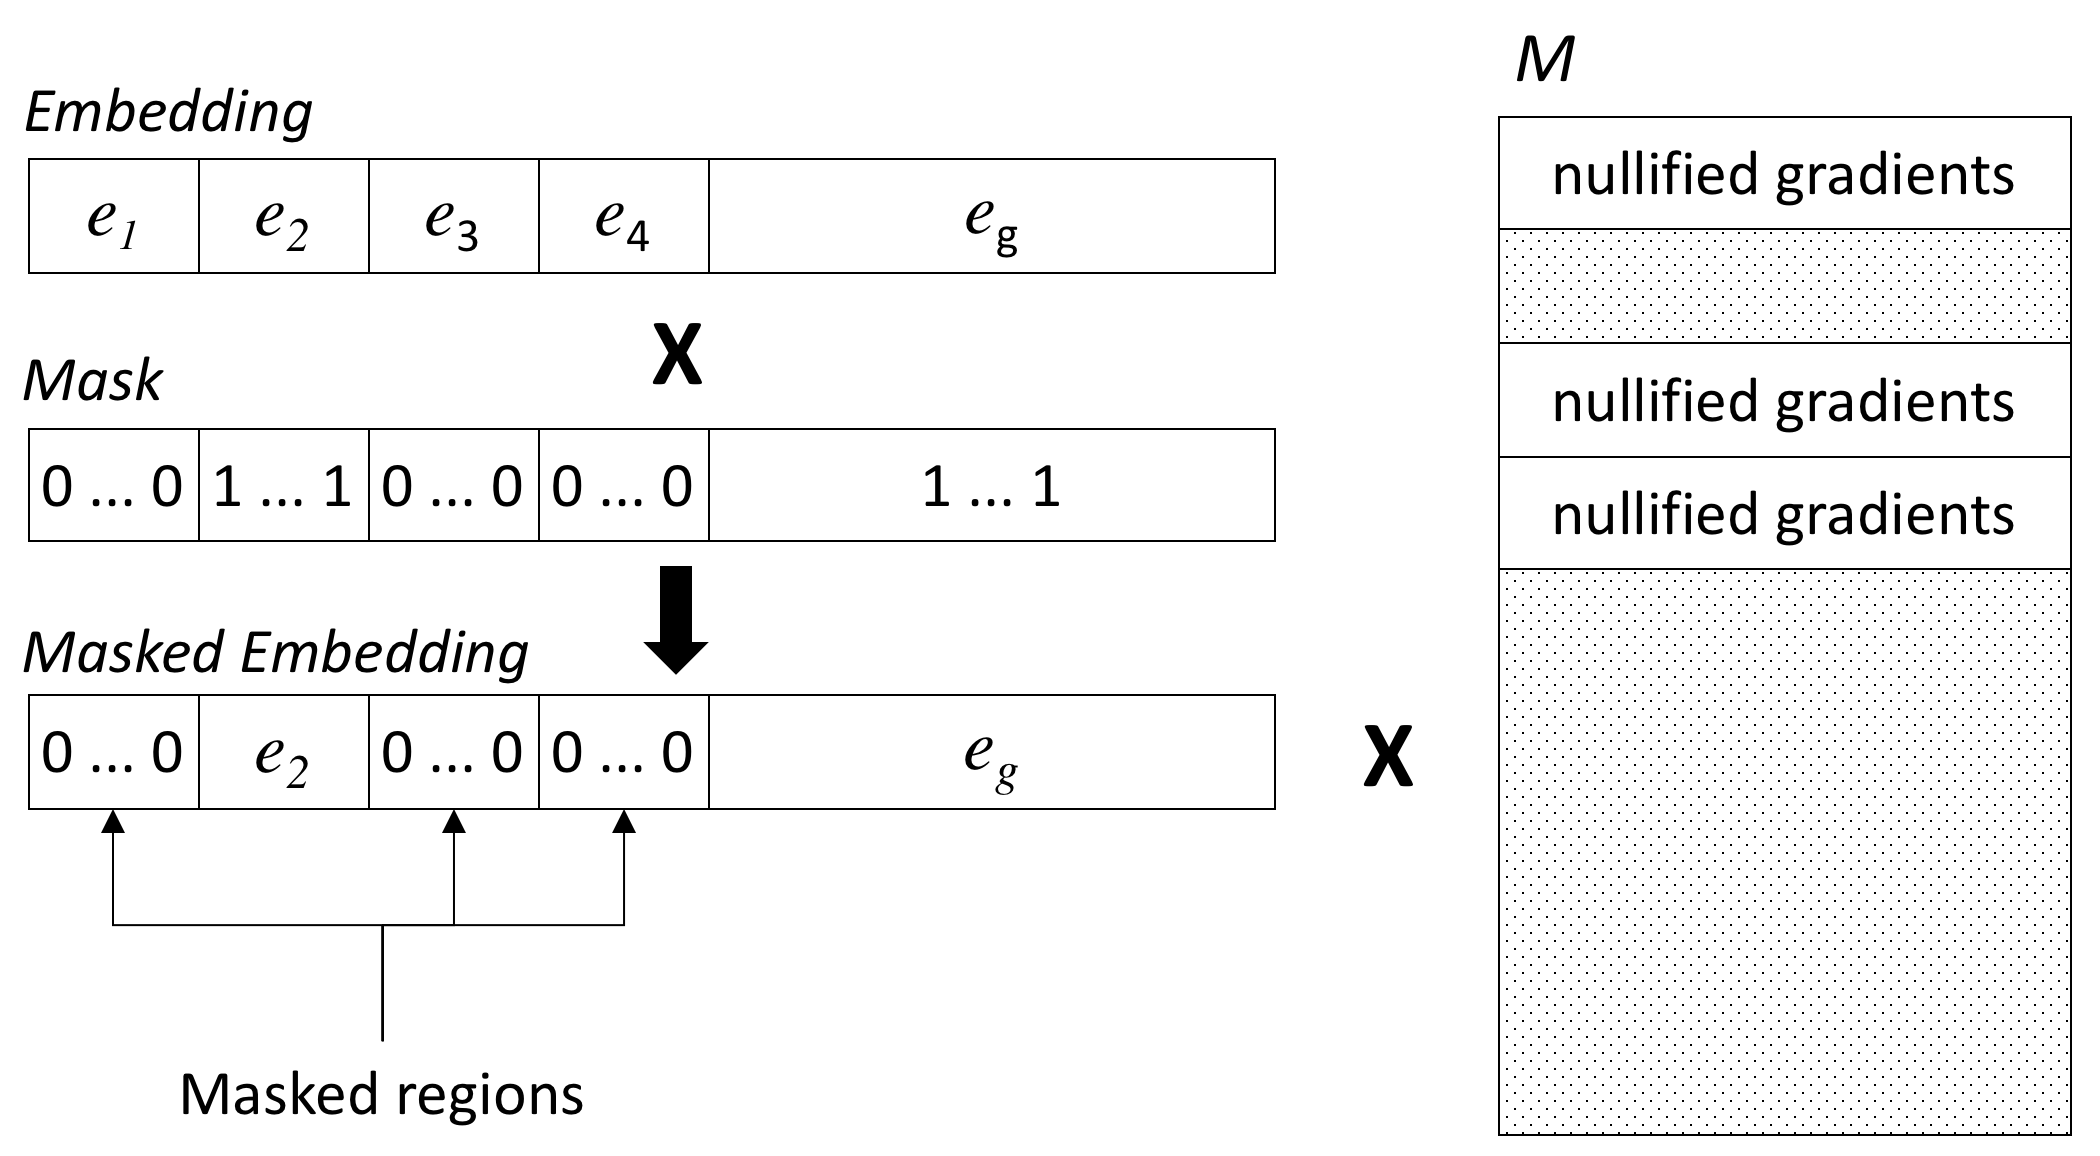
\includegraphics[width=0.6\textwidth]{graphics/embeddings}
  \caption{Lexicalized domain embeddings. When processing a sample from domain $2$, we only activate the corresponding parameter region ($\theta_2$) in the input embeddings; the remaining domain-specific parts are zeroed out and do not receive any update. The domain-agnostic part is always active and is updated irrespective of the input domain.} 
  \label{fig:network-chap5}
\end{figure}

Ensuring that the actual embedding does not contain any zero is essential for the Transformer model since the lexical representations are added to the positional encoding, which would undo the effect of domain masking and propagate a gradient even to regions that should not be modified. With our design, we make sure that the matrix $M$ receives gradient $0$ at regions corresponding to deactivated regions in the word embedding during backpropagation. Those regions are also masked in the forward step. Thus they do not interfere with the training on the domains to which they are not assigned (see Figure~\ref{fig:network-chap5}). Our architecture is thus readily compatible with any NMT architecture, where we replace standard embedding layers with the embeddings defined in equation~\eqref{eq:embedding-chap5}. In our experiments, we consider both the attentional RNN architecture of \citet{Bahdanau15learning} and the Transformer architecture of \citet{Vaswani17attention}.

\section{Contextualized domain representations}
\label{sec:sparse-chap5}
\system{CDR}s replace the linear combination of domain-agnostic units and domain-specific units used to compute LDR embeddings by multiplying the output of each layer with domain-specific dropping vector as follows

\begin{equation}
\begin{array}{rcl}
\tilde{h}^{l} &=& h^{l} * r^{l}(d) \\
r^{l}(d) & \in & \mathbb{R}^{d_k} \\
r^{l}(d)_i &=& \begin{cases}
      1, & \text{if}\ i<d_a \\
      1, & \text{if}\ d_a + d \times \frac{d_k - d_a}{n_d} \leq i < d_a + (d+1) \times \frac{d_k - d_a}{n_d} \\
      0, & \text{otherwise}
    \end{cases} \\
d & \in & \{0,\dots,n_d-1 \} \\
\end{array}
\label{eq:sparse-chap5}
\end{equation}
$h_l$ is the output of the $l^{th}$ layer; $d_a$ is the number of domain-agnostic nodes; $n_d$ is the number of domains. We allocate the same number of domain-specific nodes for every domain. However, the number of nodes in each intermediate layer is always fixed at $d_k$, \system{CDR} can not dynamically create more units for new domains. Therefore, the model currently only handles a fixed number of domains. In Section~\ref{sec:conclusion-chap5} we will discuss a promising approach that allows \system{CDR} to handle an arbitrary number of domains.

\begin{figure}[h!]
  \center
  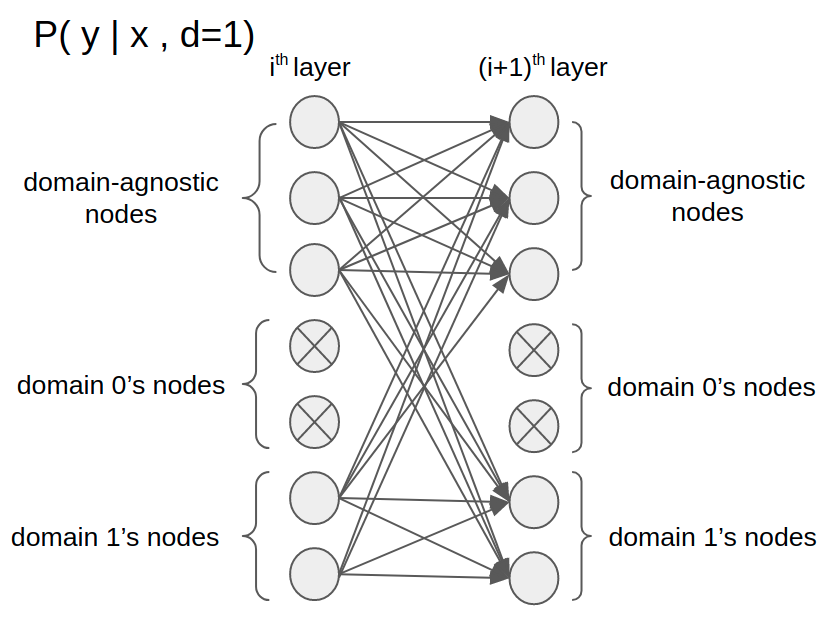
\includegraphics[width=0.6\textwidth]{graphics/Sparse_layers}
  \caption{Contextualized domain representations. When processing a sample from domain $1$, only the signal of the domain-agnostic nodes and the $1^{th}$ domain's nodes are passed to higher layers, other nodes are dropped out.} 
  \label{fig:sparse-chap5}
\end{figure}
In our experiments with \system{CDR}, we consider only the Transformer architecture and the same experimental setting as in Section~\ref{ssec:corpora-chap4}.

\section{Experiments \label{sec:experiments-chap5}}
\subsection{Domains, data and metrics \label{ssec:data-chap5}}
\subsubsection{4 domains, 2 language pairs}
We experiment with two language pairs (English-French, English-German) and data originating from three domains, corresponding to texts from three European institutions: 
the European Parlement (EPPS) \citep{Koehn05europarl}, 
the European Medicines Agency (EMEA), 
the European Central Bank (ECB) \citep{Tiedemann09news},
In addition, for English-French we also use corpora in the IT-domain obtained from the OPUS web site\footnote{\url{http://opus.nlpl.eu}} corresponding to KDE, Ubuntu, GNOME and PHP datasets (IT). Moreover, we use IT only in the scenario of continual training, in which we continue training our MDMT system with the mix of new domain IT and the old domains EMEA, ECB and EPPS.

We randomly split those corpora into training, validation and test sets (see statistics in Table~\ref{tab:Corpora-chap5}).
Validation sets are used to chose the best model according to the average BLEU score \citep{Papineni02bleu}\footnote{We use detokenized, truecasing multibleu.}

\begin{table}[h]
  \centering
  \begin{tabular}{ |llll|} %*{4}{|r|}}
    \hline
    Corpus & Train & Valid & Test \\ 
    \hline
    \multicolumn{4}{l}{English $\rightarrow$ French }\\
    %\multicolumn{4}{|l|}{Vocab size - En: 30,165, Fr: 30,398}\\
    \hline
    EMEA  & 1.09M & 1,000 & 1,000$_{(300)}$\\
    ECB    & 0.19M & 1,000 & 1,000     \\
    EPPS   & 2.01M  & 1,000 & 1,000  \\
    IT         & 0.54M  & 1,000 & 1,000 \\  
    \hline
    \multicolumn{4}{l}{English $\rightarrow$ German}\\
    %\multicolumn{4}{|l|}{Vocab size -  En:30,159, De: 30,698}\\ 
    \hline
    EMEA  & 1.11M & 1,000 & 1,000$_{(300)}$ \\
    ECB     &  0.11M & 1,000 & 1,000  \\
    EPPS   & 1.92M & 1,000 & 1,000 \\ 
    \hline
\end{tabular}
\caption{Corpora statistics.}
\label{tab:Corpora-chap5}
\end{table}

Note that the EMEA dataset distributed on the OPUS site contains multiple sentence duplicates. 
We therefore report below two numbers as $S_{(T)}$: the first ($S$) is comparable to what has been published on earlier studies (e.g. \citet{Zeng18multidomain}), the second one ($T$) is obtained by making the test entirely disjoint from the training (700~duplicated sentences are discarded).

To reduce the number of lexical units and make our systems open-vocabulary, we apply Byte-Pair Encoding \citep{Sennrich16neural} separately for each language with 30,000 merge operations.
\subsubsection{7 domains, 1 language pair}
We report again the performance of \system{LDR} in the same setting presented in Section~\ref{ssec:corpora-chap4}, which consists of 7 domains in English$\rightarrow$French translation task. For the sake of brevity, we will not provide the description of the data here (see Section~\ref{ssec:corpora-chap4}).

\subsubsection{Statistical significance}
Statistical significance is estimated using bootstrap resampling \citep{Koehn04statistical}, implemented in compare-mt\footnote{\url{https://github.com/neulab/compare-mt}} \citep{Neubig19compare-mt}. We report significant differences at the level of $p=0.05$.

\subsection{Baselines \label{ssec:baselines-chap5}}
\subsubsection{3 domains, 2 language pairs}
To validate our findings, we compared lexicalized domain embedding models with standard models using both attentional Recurrent Neural Networks (RNNs) and the Transformer architecture. Our baselines consist of:
\begin{itemize}
\item generic models trained with a simple concatenation of all corpora (\texttt{Mixed-Nat});
\item models tuned separately on each domain for respectively (10000, 15000, 5000) iterations using in-domain data (\texttt{ft$_{EMEA}$}, \texttt{ft$_{EPPS}$}, \texttt{ft$_{ECB}$}); 
\item models using domain tags as in \citet{Kobus17domain} (\texttt{DC}); 
\end{itemize}

For all models, we set the embeddings size equal to 512; the size of hidden layers is equal to 1024 for RNNs and 512 for Transformer. 
Other important configuration details are as follows:
Transformer models use multi-head attention with 8 heads in each of the 6 layers; 
the inner feedforward layer contains 2048 cells;  
RNN models use 1 layer on both sides: 
a bidirectional LSTM encoder and a unidirectional LSTM decoder with attention.
The domain control systems are exactly as their baseline counterparts (RNN and Transformer), with an additional 2 cells encoding the domain on the input layer.
 %
To train NMT systems, we use Adam, with parameters $\beta_1=0.9$, $\beta_2 = 0.999$, $\alpha=0.0005$ for RNNs; with parameters $\beta_1=0.9$, $\beta_2= 0.98$, with Noam decay \citep{Vaswani17attention} for Transformer ($warmup\_steps=4000$). In all cases, we use a batch size of~128 and a dropout rate of 0.1 for all layers. 
All our systems are implemented in OpenNMT-tf\footnote{\url{https://github.com/OpenNMT/OpenNMT-tf}} \citep{Klein17opennmt}.
\subsubsection{6 domains, 1 language pair}
The description of MDMT systems for the comparison with \system{CDR} and \system{LDR} was provided in Section~\ref{ssec:baselines-chap4} and in Section~\ref{ssec:systems-chap4}.

\subsection{Implementing Lexicalized Domain Representations}
\subsubsection{3 domains, 2 language pairs}
\label{sssec:ldr3domain-chap5}
In order to implement \system{LDR}, we split the embedding vector into four regions: 3 are domain specific and 1 is domain-agnostic, with sizes $[8,8,8,488]$ respectively. If a sentence originates from domain $i$, the domain specific regions for all domains $j \neq i$ will be zeroed out while the other regions are activated (cf. Figure~\ref{fig:network-chap5}). 
We then use a dense layer of size~512 to fuse the region for the active domain and the domain-agnostic region. Training is formalised in algorithm~\ref{alg:multidomain-chap5}.
%
Note that each iteration of algorithm \ref{alg:multidomain-chap5} uses 2~batches: a ``generic'' batch updating only the domain-agnostic region; and a ``domain-specific'' batch updating both the domain-agnostic and domain-specific parameters. 

\begin{algorithm}[h]
\caption{Multi-domain Training}
\label{alg:multidomain-chap5}
\begin{algorithmic}[1]
\REQUIRE {Corpora $C_i, i\in [1,..,d]$ for $d$ domains, Batch size $B$}%, Optimization algorithm $\operatorname{Opt}$}
\REPEAT 
\STATE{Randomly pick $i \in [1,..,d]$ w.r.t the multinomial distribution $[\frac{|C_i|}{\sum_{i\in [1,..,d]}|C_i|}]$.}
\STATE{Randomly pick $B$ sentences from $C_i$.}
\STATE{Activate only domain-agnostic region to create generic batch, denoted $W_g$.}
\STATE{Compute gradient of $\theta_s$, $\frac{\partial L}{\partial \theta_s}$ using $W_g$.}
\STATE{Activate domain-specific and domain-agnostic regions to create domain-specific batch $W_i$}
% \STATE{Pass $W_i$ to a dense layer}
\STATE{Compute gradient of domain-specific parameters $\theta_i$, $\frac{\partial L}{\partial \theta_i}$ using $W_i$.}
\STATE{Update parameters $\theta_s$ using $\frac{\partial L}{\partial \theta_s}(W_g)$ and $\theta_i$ using $\frac{\partial L}{\partial \theta_i}(W_i)$}
\UNTIL{convergence}
\end{algorithmic}
\end{algorithm}
The batch selection procedure (step~2 of algorithm~\ref{alg:multidomain-chap5}) ensures that the number of examples in each domain used in training  follows the distribution of the training data, i.e., sentences from the Europarl domain will be selected more frequently that the two other domains. We also consider a more balanced sampling procedure, where $i$ is selected according to  distribution $[\frac{\sqrt{|C_i|}}{\sum_{i\in [1,..,d]}\sqrt{|C_i|}}]$. The corresponding results are reported as \texttt{LDR}$^{0.5}$.
\subsubsection{6 domains, 1 language pair}
\label{sssec:ldr6domain-chap5}
In this setting, we split the embedding vector of size $532$ into seven regions: 6 are domain specific and 1 is domain-agnostic, with sizes $[4,4,4,4,4,4,508]$ respectively. By doing this, each domain will have 512 effective units. A dense layer maps the resulted sparse \system{LDR} embedding to an embedding of $512$ units before passing to the encoder/decoder.

\subsection{Implementing Contextualized domain representations}
\subsubsection{6 domains, 1 language pair}
We do nothing special except applying domain dropping mask to each layer as explained in Equation ~\eqref{eq:sparse-chap5} in both the encoder and the decoder of an NMT model. For the hyperparameters, we choose heuristically $d_a = 480$ and $d_k = 672$ so that there are $\frac{672-480}{6} = 32$ domain-specific nodes for each domain, making the effective number of nodes for each domain equal to $512$. This setting uses approximately $3m$ additional parameters per domains, which is only $25\%$ compared to \system{FT-Res} and \system{MT-Res} (see Section~\ref{ssec:cost-chap4} and Table ~\ref{tab:performance-chap4}).

In our experiments, we evaluate this method with Transformer models, which are state-of-the-art architecture in MT. We also report \texttt{CDR}$^{1.0}$ and \texttt{CDR}$^{0.5}$ which correspond to the distribution of simple concatenation of the domains' corpus and the down-sampling distribution $[\frac{\sqrt{|C_i|}}{\sum_{i\in [1,..,d]}\sqrt{|C_i|}}]$.

\subsection{Results \label{ssec:results-chap5}}
\subsubsection{3 domains, 2 language pairs}
\label{sssection:3domain-chap5}
Results are summarized respectively in Table~\ref{tab:results-trsf-chap5} for the Transformer systems and Table~\ref{tab:results-rnn-chap5} for the RNN systems\footnote{As explained above, we  report two numbers when testing with EMEA, except for the fine-tuning scenarios when tuning on ECB and EPPS.}. First, we observe that Transformers are consistently better than RNNs and that fine-tuning on a domain-specific corpus, when applicable, is almost the best way to optimize the performance on that domain.\footnote{This is not so clear for EPPS, where fine-tuning does not seem to help.}  
Note that fine-tuning however yields a marked (even sometimes catastrophic, eg.\ for the EMEA-tuned Transformer system) decrease in performance for the other domains. 

Our approach (\texttt{LDR}$_{oracle}$) is consistently better than the \texttt{Mixed-Nat} strategy, with gains that range from very large (for EMEA and ECB) to unsignificant (for EPPS in most conditions). 
This means that our architecture is somehow able to compensate for the data unbalance and to raise the performance of the multi-domain system close to the best (fine-tuned) system in each domain. 
We even observe rare cases where the \texttt{LDR}$_{oracle}$ system outperforms fine-tuning (e.g.\ Transformer en:de in the EMEA domain). 
\texttt{LDR}$_{oracle}$ is also better than Domain Control in three conditions out of four, \texttt{DC} being seemingly a better choice for the RNN than for the Transformer architecture. 
As expected, ignoring the true domain label yields a light drop in performance: this is reflected in the results of \texttt{LDR}$_{pred}$, which relies on automatically predicted domain labels.\footnote{Our domain classifier uses a bi-LSTM RNN encoder, followed by a simple softmax layer. 
Its precision on a development set exceeds 95\%.}
Note that this decrease is however hardly significant, showing that our architecture is quite robust to noisy labels. 
Even in the worst case scenario where all domain tags are intentionally wrong (\texttt{LDR}$_{wrong}$), we see that the domain-agnostic part still ensures a satisfying level of performance. 
A last contrast is with \texttt{LDR}$_{oracle}^{0.5}$ where we change the distribution of training sentences to decrease the weight of EPPS data and increase the number of ECB samples. 
As a result, we see a small decrease for EMEA and EPPS, and a large boost for ECB. 
This shows that our technique can be used in conjunction to other well known strategies for performing domain adaptation. 

\begin{table}[!h]
\begin{center}
\scalebox{1.0}{
\begin{tabular}{|l|lcc|c|}
\hline
Model & EMEA & EPPS & ECB & Avg. \\
\hline
%\multicolumn{8}{l}{} \\[-9pt]  
\multicolumn{5}{l}{English$\rightarrow$French} \\
\hline
$\mathtt{Mixed-Nat}$          & 67.69$_{47.60}$ & 37.50 & 53.49 & 52.89\\
\hline
$\mathtt{FT}_{EMEA}$ & 76.77$_{49.43}$ & 17.16 & 11.99 & 35.30\\
$\mathtt{FT}_{EPPS}$  & 20.86 & 37.04 & 24.53 & 27.47\\
$\mathtt{FT}_{ECB}$    & 26.93 & 27.09 & \bf 56.52 & 36.84\\
\hline
$\mathtt{DC}$              & 67.87$_{45.42}$ & 37.31 & 54.14 & 53.10\\
\hline
$\mathtt{LDR}_{oracle}$            & 74.26$_{\bf 49.90}$ & 37.67 & 54.07 & 55.33\\
$\mathtt{LDR}_{oracle}^{0.5}$   & \bf 74.95$_{49.38}$ & 37.35 & 55.91 & \bf 56.07\\
%$\mathtt{LDR}_{generic}$          & 73.97$_{49.54}$ & 37.81 & 53.67 & \\
$\mathtt{LDR}_{pred}$               & 74.29$_{49.84}$ & \bf 37.73 & 54.01 & 55.34\\
$\mathtt{LDR}_{wrong}$            & 72.95$_{49.78}$ & 37.62 & 53.35 & 54.64\\
  \hline
%\multicolumn{8}{l}{} \\[-9pt]
\multicolumn{5}{l}{English$\rightarrow$German} \\
\hline
$\mathtt{Mixed-Nat}$         & 64.57$_{42.99}$ & 26.47 & 68.67 & 53.23\\
\hline
$\mathtt{FT}_{EMEA}$ & 68.35$_{42.97}$ & 17.02 & 32.87 & 39.41\\
$\mathtt{FT}_{EPPS}$  & 36.19 & 26.29 & 40.71 & 34.39\\
$\mathtt{FT}_{ECB}$   & 24.72 & 18.36 & \bf 74.05 & 39.04\\
\hline
$\mathtt{DC}$ & 63.48$_{42.98}$ & 26.27 & 66.95 & 52.23\\
\hline
$\mathtt{LDR}_{oracle}$ & 70.90$_{\bf 46.12}$ & 26.30 & 68.90 & 55.36\\
$\mathtt{LDR}_{oracle}^{0.5}$ & \bf 71.31$_{45.23}$ & 25.98 & 73.74 & \bf 57.01\\
%$\mathtt{LDR}_{generic}$ & 70.86$_{45.60}$ & 26.14 & 68.59 & \\
$\mathtt{LDR}_{pred}$ & 70.89$_{\bf 46.12}$ & \bf 26.53 & 68.63 & 55.35\\
$\mathtt{LDR}_{wrong}$ & 69.51$_{43.50}$ & 26.31 & 66.86 & 54.22\\
\hline
\end{tabular}
} %scalebox
\end{center}
\caption{BLEU scores for  Transformer systems \label{tab:results-trsf-chap5}. Boldface denotes significant gains with respect to $\mathtt{Mixed-Nat}$.}
\end{table}

\begin{table}[!h]
\begin{center}
\scalebox{1.0}{
\begin{tabular}{|l|lcc|c|}
\hline
Model & EMEA & EPPS & ECB & Avg. \\
\hline
%\multicolumn{8}{l}{} \\[-9pt]
\multicolumn{5}{l}{English$\rightarrow$French} \\
\hline
$Mixed-Nat$                         & 65.42$_{45.11}$ & 34.70 & 51.38 & 50.50\\
\hline
$\mathtt{FT}_{EMEA}$   & 72.06$_{\bf 47.33}$ & 18.62 & 16.78 & 35.82\\
$\mathtt{FT}_{EPPS}$    & 35.47$ $ & 34.61 & 39.56 & 36.55\\
$\mathtt{FT}_{ECB}$      & 21.93$ $ & 22.60 & 51.53 & 32.02\\
\hline
$\mathtt{DC}$                            & 68.26$_{43.76}$ & 35.13 & 50.09 & 51.16\\
% \hline
%$\mathtt{WDCMT}$           & 68.76$_{45.29}$ & 35.71 & 52.75 & \\
\hline
$\mathtt{LDR}_{oracle}$            & 71.73$_{46.30}$ & \bf 35.21 & 50.91 & 52.62\\
%$\mathtt{LDR_{condgru}}_{pred}$   & 71.7$_{46.21}$ & 35.09 & 51.22 & \\
$\mathtt{LDR}_{oracle}^{0.5}$   & 71.70$_{46.41}$ & 34.24& \bf 52.37 & \bf 52.77\\
%$\mathtt{LDR}_{generic}$          & 70.59$_{46.37}$ & 35.22 & 49.68 & \\
$\mathtt{LDR}_{pred}$               &\bf 72.76$_{46.35}$ & 35.10 & 50.38 & 52.75\\
$\mathtt{LDR}_{wrong}$            & 62.10$_{43.29}$ & 34.17 & 48.79 & 48.35\\
\hline
%\multicolumn{8}{l}{} \\[-9pt]
\multicolumn{5}{l}{English$\rightarrow$German} \\
\hline
$Mixed-Nat$                        & 57.37$_{37.94}$ & 23.10 & 63.54 & 48.00\\
\hline
$\mathtt{FT}_{EMEA}$  & 65.64$_{\bf 44.71}$ & 12.36 & 15.93 & 31.31\\
$\mathtt{FT}_{EPPS}$   & 24.90$ $ & 22.98 & 26.26 & 24.71\\
$\mathtt{FT}_{ECB}$     & 41.80$ $ & 15.97 & 71.07 & 42.95\\
\hline
$\mathtt{DC}$                & 62.53$_{39.25}$ & \bf 23.74 & 65.71 & 50.66\\
%\hline
%$\mathtt{WDCMT}$ & 64.05$_{38.54}$ & 22.82 & 67.00 & \\
\hline
$\mathtt{LDR}_{oracle}$     & \bf 63.43$_{40.04}$ & 22.66 & 64.40 & 50.16\\
$\mathtt{LDR}_{oracle}^{0.5}$   & 63.27$_{38.16}$ & 21.83 & \bf 69.55 & \bf 51.55\\
%$\mathtt{LDR}_{generic}$   & 63.27 $_{39.75}$ & 22.62 & 63.70 & \\
$\mathtt{LDR}_{pred}$        & 63.17$_{39.92}$ & 22.51 & 64.00 & 49.89\\
$\mathtt{LDR}_{wrong}$     & 56.84$_{37.05}$ & 22.06 & 61.66 & 46.85\\
\hline
\end{tabular}
} %scalebox
\end{center}
\caption{BLEU scores for RNN systems\label{tab:results-rnn-chap5}}
\end{table}
% \clearfloat

We also compare our architecture with the multi-domain model of \citet{Zeng18multidomain} (\texttt{WDCMT}) for the pair English$\rightarrow$French. We use the author's implementation\footnote{\noindent\url{http://github.com/DeepLearnXMU/WDCNMT}} that is composed of one bidirectional Gated recurrent units (GRU) layer on the encoder side; and one unidirectional conditional GRU layer on the decoder side; the dimension of ``domain'' layers is~300.
%
The direct comparison with our RNN is difficult, as both networks differ in many ways: framework, cell types, \textit{etc}. Results in Table~\ref{tab:results-rnn-wdcmt-chap5} therefore use a variant of our model that makes it more similar to the \texttt{WDCMT} network. In particular, this variant also uses a single GRU layer in the encoder and a single conditional GRU layer in the decoder ($\mathtt{LDR}_{pred}^{condgru}$). As can be seen in this table, our model is on average comparable to \texttt{WDCMT}, while using a much simpler design.

\begin{table}[!h]
\begin{center}
\scalebox{1.0}{
\begin{tabular}{|l|ccc|c|}
\hline
Model & EMEA & EPPS & ECB & Avg. \\
\hline
%\multicolumn{8}{l}{} \\[-9pt]
\multicolumn{5}{l}{English$\rightarrow$French} \\
\hline
$\mathtt{LDR}_{pred}$                   & \bf 72.76$_{46.35}$ & 35.10 & 50.38 & \bf 52.75\\
$\mathtt{LDR}_{pred}^{condgru}$  & 71.70$_{46.21}$ & 35.09 & 51.22 & 52.67\\
$\mathtt{WDCMT}$                        & 68.76$_{45.29}$ & \bf 35.71 & \bf 52.75 & 52.40\\
\hline
\end{tabular}
} %scalebox
\end{center}
\caption{BLEU scores for RNN systems. Comparison between \texttt{WDCMT} and $\texttt{LDR}_{pred}$ built using conditional GRUs.\label{tab:results-rnn-wdcmt-chap5}}
\end{table}
\subsubsection{6 domains, 1 language pair}
To allow the readers easily compare the performance of \system{LDR} between 2 settings: 4 domains and 6 domains, we report again a part, which contains only Transformer-based system, of Table ~\ref{tab:performance-chap4} (see Table ~\ref{tab:mdmt-res-chap5}).
\begin{table*}
  \centering
  \begin{tabular}{|p{4cm}|*{8}{r|}} \hline
%     &&&&&& \\
    Model / Domain & \multicolumn{1}{c|}{\domain{ med}} & \multicolumn{1}{c|}{\domain{ law}} & \multicolumn{1}{c|}{\domain{bank}} & \multicolumn{1}{c|}{\domain{talk}} & \multicolumn{1}{c|}{\domain{ it }} & \multicolumn{1}{c|}{\domain{ rel}} & \multicolumn{1}{c|}{w\domain{avg}} & \multicolumn{1}{c|}{\domain{avg}} \\ \hline % & \multicolumn{1}{c|}{\domain{news}} 
    \system{Mixed-Nat}  \hfill{\footnotesize[65m]} & 37.3 & 54.6 & 50.1 & 33.5 & 43.2 & 77.5  & 41.1  & 49.4 \\% & 23.5\\
    \system{Mixed-Bal}   \hfill{\footnotesize[65m]} &  35.3 & 54.1 & 52.5 & 31.9 & 44.9 & 89.5 & 40.3  & 51.4 \\ %& \\
    \system{FT-Full}       \hfill{\footnotesize[6$\times$65m]} & 37.7 & \SB{59.2} & \SB{54.5} & 34.0 & \SB{46.8} & \SB{90.8}   & \SB{42.7} & \SB{53.8} \\ \hline
 %   Full-finetuned on extended in-domain corpora (news) & && 33.96&&& & &\\nn
    \system{DC-Tag} \hfill{\footnotesize[+6$\times$512]}        & 38.1 & 55.3 & 49.9   & 33.2 & 43.5 & \SB{80.5} &41.6 & 50.1    \\%    & 21.8 \\
    \system{DC-Feat} \hfill{\footnotesize[+6$\times$4]}    & 37.7  & 54.9 & 49.5   & 32.9 & 43.6 & \SB{79.9} &41.4 & 49.9   \\% & \SW{21.7} \\
    \system{LDR}       \hfill{\footnotesize[+6$\times$384k]}    & 37.0   & 54.7 & 49.9 & 33.9 & 43.6 & \SB{79.9} &40.9 & 49.8          \\% & 22.1 \\ 
    \system{CDR}$^{1.0}$ \hfill{\footnotesize[+6$\times$3m]} & 38.0 & \SB{55.9} & \SB{51.4} & 33.9 & \SB{45.0} & \SB{87.4} & \SB{42.4} & 51.9 \\
    \system{CDR}$^{0.5}$ \hfill{\footnotesize[+6$\times$3m]} & 37.3 & \SB{57.0} & \SB{54.5} & 32.2 & \SB{47.6} & \SB{91.0} & \SB{42.4} & 53.3 \\
    \system{TTM}      \hfill{\footnotesize[+6$\times$1024]}        & 37.3 & 54.9 & 49.5 & 32.9 & 43.6 & \SB{79.9} &41.0 & 49.7     \\% &  23.4 \\
    \system{DM}        \hfill{\footnotesize[+0]}         & \SW{35.6} & \SW{49.5}  & \SW{45.6}& \SW{29.9} & \SW{37.1} & \SW{62.4} & 38.1 & 43.4 \\ % & 22.6\\
    \system{ADM}      \hfill{\footnotesize[+0]}         & 36.4 & \SW{53.5}  & \SW{48.3} & \SW{32.0} & \SW{41.5} & \SW{73.4} & 38.9 & 47.5 \\% & 23.3 \\
    \revisiondone{\system{FT-Res}}   \hfill{\footnotesize[+6$\times$12.4m]}  & 37.3 & \SB{57.9} & \SB{53.9} & 33.8 & \SB{46.7} & \SB{90.2}  & \SB{42.3} & \SB{53.3} \\ % & 20.5\\ \hline
    \system{MT-Res} \hfill{\footnotesize[+6$\times$12.4m]}    & 37.9 & \SB{56.0}  & \SB{51.2}   & 33.5   &  44.4  & \SB{88.3} & 42.0 & \SB{51.9} \\%  & \SW{21.2} \\
     \hline 
  \end{tabular}
  \caption{Translation performance of MDMT systems based on the same Transformer architecture. The former contains 65m parameters. For each system, we report the number of additional domain specific parameters, BLEU scores for each domain, domain-weighted (w\domain{avg}) and unweighted (\domain{avg}) averages. For weighted-averages, we take the domain proportions from Table~\ref{tab:Corpora-chap4}. Boldface denotes significant gains with respect to \system{Mix-Nat}, underline denotes significant losses.}
  \label{tab:mdmt-res-chap5}
\end{table*}

In this setting, \system{LDR} is only slightly better than the generic model \system{Mixed-Nat}, which is trained with the same sampling distribution. The system is only significantly better than \system{Mixed-Nat} in \domain{rel}. Moreover, \system{LDR} achieves a performance equivalent to \system{DC-Tag}, \system{DC-Feat}. This result is inconsistent with the results in the previous setting with only four domains. This might be explained by the interference between domains in the contribution of parameters in the prediction. As there are more domains and the domains' sizes are much more unbalanced, the partition of the parameters should be more extensive than the word embedding level. Moreover, word-embeddings do not capture the context, which is more important for the prediction than the word alone. We find that a partition of intermediate nodes in higher layers captures better the statistical bias than just in the $0^{th}$ layer, where the context is not formed. Our hypothesis is supported by the performance of \system{CDR}$^{1.0}$. Our model significantly outperforms \system{Mixed-Nat} in $4/6$ domains except for \domain{talk} and \domain{med} which are "hard" domains where no MDMT systems significantly does better than \system{Mixed-Nat}. Moreover, \system{CDR}$^{1.0}$ performs equivalently to \system{MT-Res} using $75\%$ less additional parameters. Furthermore, with a sampling strategy more balanced, \system{CDR}$^{0.5}$ matches the performance of \system{FT-Res}, which is carefully fine-tuned for each domain.

However, Table ~\ref{tab:redomains-chap4} shows a dramatic loss in the random domain tag setting, which means \system{LDR} is not robust in the case of 6 domains. This observation is inconsistent with the results in Table \ref{tab:results-trsf-chap5}. This loss might be due to the fact that this MDMT setting is much more adverse than the previous setting with only 3 domains. This again illustrates the need to use a wide range of available domains to evaluate the systems.

\section{Complementary experiments\label{sec:Discussion-chap5}}
\subsection{Balancing domain-agnostic and domain-specific representations in \system{LDR}\label{secc:region_size-chap5}}
An important practical question concerns the balance between the domain-agnostic and the domain-specific part of the embeddings. 
In the limit where the domain specific part is very small, we should recover the performance of the \texttt{Mixed-Nat} system; 
conversely, we expect to see a less effective sharing of data across domains by increasing the domain-specific regions. 
Table~\ref{tab:embedding-size-chap5} reports the result of  a series of experiments for the Transformer architecture (English-French) with varying domain-specific sizes allocating between 4 and 64 cells for domain-specific information, and the complement to 512 for the domain-agnostic part. 
The differences are overall quite small in our experimental setting, where the training data is relatively limited and does not require to use a large embedding size. 
We therefore decided to allocate $8$~cells for the domain specific part in the experiments of Section~\ref{sssec:ldr3domain-chap5}. 
This suggests that we could easily accommodate more domains with the same architecture and even reserve some regions to handle supplementary data (see below). %incoming training data.  
% \fyTodo{Easily accomodate more domains}
\fyDone{Given the ways embeddings are computed, why not add more domains, and test robustness agains data presentation order ?}

\begin{table}[!h]
\begin{center}
\scalebox{1.0}{
\begin{tabular}{|l|ccc|c|}
\hline
$\mathtt{LDR}_{oracle}$ & EMEA & EPPS & ECB & Avg. \\
\hline
\multicolumn{5}{l}{English$\rightarrow$French} \\
\hline
 size=4   & 74.65$_{49.61}$ & 37.42 & 54.49 & 55.52\\
 size=8   & 74.26$_{49.90}$ & 37.67 & 54.07 & 55.33\\
 size=16 & 74.15$_{49.10}$ & \bf 37.78 & \bf 54.56 & 55.50\\
 size=32 & \bf 75.10$_{48.61}$ & 37.64 & 54.29 & \bf 55.68\\
 size=64 & 74.50$_{\bf 50.17}$ & 37.27 & 54.50 & 55.42\\
\hline
\end{tabular}
} %scalebox
\end{center}
\caption{BLEU scores for the Transformer architecture for varying domain-specific embedding sizes \label{tab:embedding-size-chap5}}
\end{table}

\subsection{Additional domain setting with \system{LDR} \label{ssec:additional_domain-chap5}}
\subsubsection{4 domains}
We now evaluate the ability of our model to integrate new domains, a very common scenario for industrial MT. In this setting, we consider that we have a model ($\mathtt{LDR}_{oracle}$) trained as before for EMEA, EPPS and ECB during 200,000 iterations, which needs to process new training data from the IT domain. Assuming that we have reserved extra empty embedding cells\footnote{For this experiment, word embeddings contain 480 cells for the domain-agnostic region and 32 cells for domain specific regions (8 cells x 4 regions).} for this domain, we resume training with 4 domains during 100,000 additional iterations, yielding an updated model  $\mathtt{LDR}_{oracle}^*$. Results for the English$\rightarrow$French language pair are in Table~\ref{tab:add-chap5}, where for comparison purposes we also report numbers obtained with continued training with the $\mathtt{Mixed-Nat}$ model, training for the same number of iterations and using the same four datasets ($\mathtt{Mixed-Nat}^*$).

\begin{table}[!h]
\begin{center}
\scalebox{0.9}{
\begin{tabular}{|l|cccc|c|}
\hline
Model & EMEA & EPPS & ECB & IT & Avg.\\
\hline
\multicolumn{5}{l}{English$\rightarrow$French} \\
\hline
$\mathtt{Mixed-Nat}$                & 67.69$_{47.60}$ & 37.50 & 53.49 & 13.91 & 43.15\\
$\mathtt{Mixed-Nat}^*$             & 66.49$_{45.79}$ & 37.59 & 55.07 & 51.78 & 52.73\\
\hline
$\mathtt{LDR}_{oracle}$     & 74.26$_{\bf 49.90}$ & \bf 37.67 & 54.07 & 13.40 & 44.85\\
$\mathtt{LDR}_{oracle}^*$  & \bf 76.17$_{49.71}$ & 37.48 & \bf 55.12 & \bf 55.24 & \bf 56.00\\
\hline
\end{tabular}
} %scalebox
\end{center}
\caption{BLEU scores for the Transformer architecture when including IT as additional domain \label{tab:add-chap5}}
\end{table}

As expected, a huge improvement in performance is observed for the IT test set when learning includes in-domain data for both models, with $\mathtt{LDR}_{oracle}^*$ outperforming $\mathtt{Mixed-Nat}^*$ by a wide margin.
%
It is interesting to see that this additional data has also a positive impact on other test sets: both models similarly increase their performance for the ECB domain, and $\mathtt{LDR}_{oracle}^*$ additionally improves the results for the EMEA test, which is not the case for $\mathtt{Mixed-Nat}^*$;
finally, using IT data does not impact the quality of translations for the EPPS domain of any of the models. Overall better results are obtained by our $\mathtt{LDR}_{oracle}^*$ model trained with data from an additional source.

\subsubsection{7 domains}
We report again the result of the experiments in the continuous learning presented in Section~\ref{ssec:continual-chap4}. We observe a significant loss of \system{LDR} compared to the generic baseline \system{Mixed-Nat} while adding domain \domain{news}. The loss is mainly due to a decrease of \system{LDR}'s performance in the largest \domain{med} domain. This result shows the brittleness of our system against the change of train data distribution, in which the proportion of \system{med} drops $5\%$ from $0.68$ to $0.65$.

\subsection{Analysis of Word Embeddings of \system{LDR} \label{ssec:word_embeddings-chap5}}
One of our main assumptions is that the difference between domains can be confined at the lexical level, warranting our decision to specialize lexical representations for each domain, while the remaining part of the network is shared across domains. Linguistically, this assumption relates to the classical ``one sense per collocation'' \citep{Yarowsky93onesense} and corresponds to the fact that in many cases, polysemy corresponds to variation of use across domain. This variation of senses was reported in \citet{Carpuat13domain} as a source of errors when translating in unseen domains. The authors demonstrated that a word would be translated to different translations with respect to the domains. SMT models can not boostrap this lack of knowledge and make sense errors. In MDMT, MT models cope the same problem. In the weaker form of \citep{Yarowsky93onesense}'s theory, it allows us to assume that all occurrences of a given form in a given domain correspond to the same sense and share the same representation; the same form occurring in different domains is allowed to have one distinct embedding per domain, which may help capture polysemy and lexical ambiguity in translation. 

To check this hypothesis, we performed the following analysis of embeddings learned with the multi-domain Transformer system for English:French. For each unit\footnote{In this study, we work with BPE units, in many cases we observe the variation of use of \emph{word parts}. As we work with a large inventory, many of these units still correspond to actual words and we focus on these in our comments. We also restrict our analysis to words that occur at least 30 times in each domain, to ensure that each domain-specific region is updated during training.} in our English dictionary, we compute the $k$ nearest neighbours for each domain $i \in [1\dots{}d]$, where the distance between unit $u$ and $v$ for domain $i$ is the cosine distance in the corresponding embedding space, ie.\ assuming that the actual embedding of $v$ for domain $i$ is $e(v,i) = M_ge_g(u) + M_ie_i(v)$ (cf.\ equation~\eqref{eq:embedding-chap5}). This process yields $d$ lists of $k$ nearest neighbours. A small intersection should then be a sign of a variation of use across domains; conversely, an near-identical set of neighbours across domains should reflect the stability of word use. Table~\ref{tab:embeddings-chap5} list the 10 units with the smaller (respectively larger) intersection (we use $k=10$ and $d=3$). 

\begin{table}[h]
  \centering
%  \begin{tabularx}{1.0\linewidth}{c|c}
  \begin{tabular}{c|c}
    Polysemic ``words'' & Monosemic ``words'' \\ \hline
     ases (0) &               obtain (10) \\       
     impairment (1) &     virtually (10) \\    
     convenience (1) &    represent (10) \\    
     oring (1) &              safety (10) \\       
     ums (1) &               defence (10) \\      
     turnover (1) &         coordinated (10) \\  
     occurrence (1) &     handling (10) \\     
     tent (2) &               July (10) \\         
     ture (2) &               previous (10) \\     
     mation (2) &           better (10) \\ \hline
  \end{tabular}
  \caption{Analyzing the variation of embeddings across domains. For each word or subword we also report the size of the intersection (between 0 and 10).}
  \label{tab:embeddings-chap5}
\end{table}

Let us first consider the full words in the left column of Table~\ref{tab:embeddings-chap5}. The case of \emph{impairment} is pretty clear, occuring in EMEA mostly in terms such as ``hepatic impairment'' or ``renal impairment'', and translating into French as \textsl{insuffisance}. In ECB, its collocates are quite different and impairment often occurs in terms such as ``cost subject to impairments'' (French: \emph{co\^ut soumis \`a des r\'eductions de valeur}). Likewise, ``convenience'' seems to have its general meaning (``for convenience'') in EMEA, but appears in ECB in the specific context of ``convenience credit card'' (French: \textsl{carte de cr\' edit \`a remboursement diff\'er\'e}). We finally see the same phenomena with ``turnover'', which is consistently translated with its economic meaning (French: \textsl{chiffre d'affaire}) in ECB and EPPS, but whose collocates in EMEA ("bone turnover", ``hepatic turnover'') are associated with the idea of the cell renewall process, yielding translations such as \textsl{remodelage osseux} in French. Subword units can be analysed in the same ways: ``ums'', for instance, appears in words such as ``gums'', ``serums'', ``vacuums''  in EMEA; in ECB, ``ums'' is mostly the suffix of ``maximums'', ``minimums'', or ``premiums''; EPPS finally contains a more diverse set of ``-ums'' ending words (``stadium'', ``forum'', equilibrium'', etc). 

Let us now consider the list of putative monosemic words (on the right part of Table~\ref{tab:embeddings-chap5}), ie.\ words for which the nearest neighbors are the same in all domains. This list contains mostly words for which we do not expect much variation in translation: adjectives (``previous'', ``better''), adverbs (``virtually``), generic verbs (``handling'', ``coordinated''). Further down this list, we will also find prepositions (``at'', ``in''), auxiliary (``been'') etc.  

\section{Conclusions and outlook}
\label{sec:conclusion-chap5}
In this chapter, we have presented two new techniques for multi-domain machine translation: \system{LDR} embeddings, which is a result of adapting the ``frustratingly easy'' idea of \citet{Daume07frustratingly} to NMT architectures; \system{CDR}, which is an extension of \system{LDR} to higher layers of the NMT model. 

Our experiments have shown that for both architectures (Transformer and RNN) and two language pairs, \system{LDR} improves over the simple \system{DC-Tag} system and standard Transformer and that it is robust to noise in domain labels. However, the improvement is still limited in a mild situation where the number of domains is low, and there is less heterogeneity. Our second proposal system \system{CDR} outperforms many MDMT systems except \system{FT-Res}, which is carefully fine-tuned for each domain in a highly heterogeneous MDMT setting. However, this version of \system{CDR} handles only a fixed number of domains.

Furthermore, it is noticeable that these results are obtained without impacting the architecture or training complexity, making our approach an effective baseline for further studies in multi-domain translation. We have also shown that \system{LDR} can dynamically handle new domains; and that its domain-specific embeddings often reflect differences of "stand-alone" senses. 

In our future work, we aim to develop another version of \system{CDR} using learnable domain-node allocations which allows the method to accommodate an arbitrary number of domains.

%As mentioned in Section ~\ref{sec:sparse-chap5}, we discuss here a variant of \system{Sparse} that handles an arbitrary number of domains. We reuse the notations of Equation \eqref{eq:sparse-chap5}. We replace the hard-coded $r^{l}(d)$ dropping mask for domain $d$ by a learnable dropping mask as follows
%\begin{equation}
%\begin{array}{rcl}
%\tilde{r}^{l}(d)_i &=& \begin{cases}
%      1, & \text{if}\ i<d_a \\
%      1, & \text{if}\ d_a + p \times \frac{d_k - d_a}{n_p} \leqslant i < d_a + (p+1) \times \frac{d_k - d_a}{n_p} \  \text{AND} \  m^d(p) == 1 \\
%      0, & \text{otherwise}
%    \end{cases} \\
%p & \in & \{0,\dots,n_p-1 \} \\
%d & \in & \{0,\dots,n_d-1 \} \\
%m^d & \in & \{0,1\}^{n_p} \ \forall d \\
%\mid m^d \mid_{L_1} &=& k  \\
%\Delta^{n_p}_k & = & \{ m \in \{0,1\}^{n_p} | \mid m \mid_{L_1} = k \}
%\end{array}
%\end{equation}
%where $n_p$ is number of domain-specific regions; $m(d,p)$ follows a Bernoulli distribution which is parameterized and learned jointly with the parameters of the NMT model by optimizing the evidence lower bound (ELBO) \citep{kingma13variational} with Gumbel-softmax reparametrization trick \citep{jang17categorical}. The domain-specific region $p$ is allocated to domain $d$ if $m(d,p)==1$. The allocation of hidden nodes to each domain is now decided by the variables $m(p,d)$ which allow the model to accommodate an arbitrary number of domains. 

%\begin{array}{rcl} 
%log P(y|x,\theta,d) &=&log P(y, m^d |x,\theta,d) - logP(m^d|y, x,\theta,d) \\
%
%& = & \mathbb{E}_{P(m^d | \Phi^d)} \big[ log P(y, m^d | x,\theta,d) - log P(m^d | \Phi^d) \big]  + KL(P(m^d | \Phi^d) \parallel P(m^d|y, x,\theta,d)) \\
%
%& \geq & \mathbb{E}_{P(m^d | \Phi^d)} \big[ log P(y, m^d | x,\theta,d) - log P(m^d | \Phi^d) \big]  \\
%
%& = &  \mathbb{E}_{P(m^d | \Phi^d)} \big[ log P(y | x,\theta,m^d, d) \big] - KL \big( P(m^d | \Phi^d) \parallel P(m^d | x,\theta,d) \big) \\
%& = & \mathcal{L}(\theta, \Phi^d, x , y) \\
%& & \\
%Suppose \ \ \ P(m^d | x, \theta, d) &=& U(\Delta^{n_p}_k) \\
%
%\Phi_d & \in & \mathbb{R}^{n_p} \\
%
%Ind^d = \{ i_1, \cdots, i_k \} | \Phi^d & \sim &Sampling\_without\_replacement \big( softmax(\Phi^d) \big) \\
%
%m^d(i) &=& \mathbb{I}(i \in Ind^d)
%
%\end{array}

%\begin{array}{rcl}
%L(\theta, \Phi_0, \cdots, \Phi_{n_d\text{-1}}) &=& \sum_{d=0}^{n_d-1} \mathbb{E}_{x \sim \mathcal{D}_s^d, y \sim g^d(x)} \big[ \mathcal{L}(\theta,\Phi_d,x,y) \big]
%\end{array}

%\begin{array}{rcl}
%
%g_i &\sim& Gumbel(0,1) \ i.i.d \ \forall i \in \{ 0,\cdots,n_d-1 \} \\
%
%i_1, \cdots, i_k &=& Top_{k} \{ g_0 + \Phi^d_0, \cdots, g_{n_d-1} + \Phi^d_{n_d-1} \} \\
%
%m^d(i) &=& \mathbb{I}(i \in Ind^d) \\
%
%\end{array}

%\begin{array}{rcl}
% \tilde{m}^d &=&\displaystyle{\mathop{argmin}_{\substack{
%       0 \leq m_i \leq 1 \ \forall 0 \leq i \leq n_d\text{-}1 \\
%        1^{T}.m = k
%      }}} -(g+\Phi^d)^{T} . m - \tau H_b(m) \\
%& & \\
%H_b(m) &=& - \sum_i m_i log(m_i) + (1-m_i)log(1-m_i)
%\end{array}
%
%%\begin{array}{rcl} 
%
%Ind^d &=& Top_k(\Phi^d) \\
%m^d &=& \mathbb{I}(i\in Ind^d)\\
%
%y &\sim& P(.|x,\theta,m^d)
%
%\end{array}
	\chapter{Multi-domain residual adapters}
\section{Motivation}
Domain adaptation is an old and vexing problem for machine translation systems. The most common and successful approach to supervised adaptation is to fine-tune a baseline system with in-domain parallel data. Standard fine-tuning however modifies all the network parameters, which makes this approach computationally costly and prone to overfitting. A recent, lightweight approach, instead augments a baseline model with supplementary (small) adapter layers, keeping the rest of the model unchanged. This has the additional merit to leave the baseline model intact and adaptable to multiple domains. In this paper, we conduct a thorough analysis of the adapter model in the context of a multidomain machine translation task. We contrast multiple implementations of this idea using two language pairs. Our main conclusions are that residual adapters provide a fast and cheap method for supervised multi-domain adaptation; our two variants prove as effective as the original adapter model and open perspective to also make adapted models more robust to label domain errors.

\section{Introduction \label{sec:intro}}
Owing to multiple improvements, Neural Machine Translation (NMT) \cite{Kalchbrenner13recurrent,Sutskever14sequence,Bahdanau15learning,Vaswani17attention} nowadays delivers useful outputs for many language pairs. However, as many deep learning models, NMT systems need to be trained with sufficiently large amounts of data to reach their best performance. Therefore, the quality of the translation of NMT models is still limited in low-resource language or domain conditions \cite{Duh13adaptation,zoph16transfer,koehn17six}. While many approaches have been proposed to improve the quality of NMT models in low-resource domains (see the recent survey of \citet{Chu18asurvey}), full fine-tuning \cite{Luong15stanford,Neubig18rapid} of a generic baseline model remains the dominant supervised approach when adapting NMT models to specific domains.

Under this view, building adapted systems is a two-step process: (a) one first trains NMT with the largest possible parallel corpora, aggregating texts from multiple, heterogeneous sources; (b) assuming that in-domain parallel documents are available for the domain of interest, one then adapts the pre-trained model by resuming training with the sole in-domain corpus. It is a conjecture that the pretrained model constitutes a better initialization than a random one, especially when adaptation data is scarce. Indeed, studies of transfer learning for NMT such as \citet{artetxe20cross,aji20neural} have confirmed this claim in extensive experiments. Full fine-tuning, that adapts all the parameters of a baseline model usually significantly improves the quality of the NMT for the chosen domain. However, it also yields large losses in translation quality for other domains, a phenomenon referred to as ``catastrophic forgetting'' in the neural network literature \cite{Michael89catastrophic}. Therefore, a fully fine-tuned model is \emph{only useful to one target domain}. As the number of domains to handle grows, training, and maintaining a separate model for each task can quickly become tedious and resource-expensive.\fyDone{Fix this sentence.}

Several recent studies (e.g.\ \citep{Vilar18learning,Wuebker18compact,Michel18extreme,Bapna19simple}) have proposed more lightweight schemes to perform domain adaptation, while also preserving  the value of pre-trained models. Our main inspiration is the latter work, whose proposal relies on small \emph{adapter components} that are plugged in each hidden layer. These adapters are trained only with the in-domain data, keeping the pre-trained model frozen. Because these additional adapters are very small compared to the size of the baseline model, their use significantly reduces the cost of training and maintaining fine-tuned models, while delivering a performance that remains close to that of full fine-tuning.

In this paper, we would like to extend this architecture to improve NMT in several settings that still challenge automatic translation, such as translating texts from multiple topics, genre, or domains, in the face of unbalanced data distributions. Furthermore, as the notion of ``domains''  is not always well established, another practical setting is the translation of texts mixing several topics/domains. An additional requirement is to translate texts from domains unseen in training, based only on the unadapted system, which should then be made as strong as possible. 

In this context, our main contribution is a thorough experimental study of the use of residual adapters for multi-domain translation. We notably explore ways to adjust and/or regularize adapter modules to handle situations where the adaptation data is very small. We also propose and contrast two new variants of the residual architecture: in the first one (\emph{highway residual adapters}), adaptation still affects each layer of the architecture, but its effect is delayed till the last layer, thus making the architecture more modular and adaptive; our second variant (\emph{gated residual adapters}) exploits this modularity and enables us to explore ways to improve performance in the face of train-test data mismatch. We experiment with two language pairs and report results that illustrate the flexibility and effectiveness of these architectures. 

\section{Residual adapters \label{sec:res}}
In this section, we describe the basic version of the residual adapter architectures \citep{houlsby19parameter, Bapna19simple}, as well as two novel variants of this model.

\subsection{Basic architecture \label{ssec:architecture}}
\fyDone{More contexts and notations from the transformer}\fyDone{Encoder / decoder layers}

\subsubsection{The computation of adapter layers}
Our reference architecture is the Transformer model of \citet{Vaswani17attention}, which we assume contains a stack of layers both on the encoder and the decoder sides. Each layer contains two subparts, an attention layer, and a dense layer. Details vary from one implementation to another, we simply contend here that each layer $i \in \{1 \dots L\}$ (in the encoder or the decoder) computes a transform of a fixed-length sequence of $d$-dimensional input vectors $h^{i}$ into a sequence of output vectors $h^{i+1}$ as follows ($\mathbf{LN}$ denotes the (sub)layer normalization, $\mathbf{ReLU}$ is the ``rectified linear unit'' operator):\fyDone{Use align env}\fyDone{Add layer normalization, replace notation b by a}
\begin{align*}
  h^{i}_0 &= \mathbf{LN}(h^{i}) \\
  h^{i}_1 &= \mathbf{W}_{db}^{i}h_0^{i} + a^i_{1} \\
  h^{i}_2 &= \mathbf{ReLU}(h_1^{i})
  \\
%\end{align*}
%\begin{align*}
  h^{i}_3 &= \mathbf{W}_{bd}^{i}h_2^{i} + a^i_{2} \\
  \bar{h}^{i} &= h^{i}_3 + h^i.
\end{align*}
Overall, the  $i^{\text{th}}$ adapter is thus parameterized by matrices $\displaystyle{\mathbf{W}_{db}^{i}\in\mathbb{R}^{d\times b}}$,$\displaystyle{\mathbf{W}_{bd}^{i}\in\mathbb{R}^{b\times d}}$, bias vectors $\displaystyle{b^i_{1} \in \mathbb{R}^{b}}$, $\displaystyle{b^i_{2} \in \mathbb{R}^{d}}$, with $b$ the dimension of the adapter \fyDone{($d \gg b$) not true}\fyDone{Check this}. For the sake of brevity, we will simply denote $h^{i}_3 = \operatorname{ADAP}^{(i)}(h^i)$, and $\theta_{\operatorname{ADAP}^{(i)}}$ the corresponding set of parameters.\fyDone{or is it $h_i$ ?}\fyDone{attention aux matrices $W_i$}

The "adapted" hidden vectors $\bar{h}^i_{ 1\leq i \leq L-1}$, where $L$ is the number of layers, will then be the input of the $(i+1)^{\text{th}}$\fyDone{Self attention ?} layer; $\bar{h}^L$ is passed to the decoder if it belongs to the encoder side, or is the input of output layer if it belongs to the decoder side. Note that zeroing out all adapters enables us to recover the basic Transformer, with $\bar{h}^{i} = h^i$ for all $i$.

In the experiments of Section~\ref{sec:exp}, we use $2\times{}L=12$ residual adapters, one for each of the $L=6$ attention layers of the encoder and similarly for the decoder.\footnote{In the decoder, the stack of self-attention and cross encoder-decoder attention only counts as one attention layer and only corresponds to one residual adapter.}

\subsubsection{Design space and variants \label{sssec:design-space}}
This general architecture leaves open many design choices pertaining to the details of the network organization, the training procedure, and the corresponding objective function.

The first question is the number of adapter layers. While in principle, all Transformer layers can be subject to adaptation, it is nonetheless worthwhile to consider simpler adaptation schemes, which would only alter a limited number of layers. Such strategy might be especially relevant when the training data contains very small domains, as in the experiments of Section~\ref{sec:exp}, and for which a complete adaptation may not be necessary or/and or prone to overfitting. Likewise, it might be meaningful to explore ways to share subsets of adapters across domains. This, in turn, raises the issue of which layer(s) to adapt, a question that can be approached in the light of recent analyses of Transformers models, which conjecture that the higher layers encode global patterns with a more ``semantic'' interpretation, while the lower layers encode local patterns akin to morpho-syntactic information \cite{raganato18analysis}.

% The size of available corpora for each domain is extremely varying. For example, the corpus of domain \domain{tourism} in En-De contains only around $7\times10^3$ sentence pairs while the corpus of domain \domain{news} in En-De contains approximately $3\times10^6$ sentence pairs. For extremely small domains, we could economize the number of parameters by reducing the number of residual adapters in the architecture. While only a limited number of adapters are incorporated to the NMT model, which positions in the model are more important in the domain adaptation task? We would like to analyze the impact of position and number of residual adapters involved in the adapted model. It is conjectured that the higher layers represent more global patterns such as semantic while the lower layers represent more local patterns such as syntactic \cite{raganato18analysis}\fyTodo{Missing reference here}. The domain shift in local patterns and global patterns has not yet been studied. In this paper, we do not intend to study this aspect of the domain adaptation problem. We would like to give an extensive comparison between domain adaptation in different levels in the NMT model. 

A related question concerns the regularization of adapter layers to mitigate overfitting. Reducing the number of adapters, or their dimensions, is simple, but such choices are difficult to optimize numerically -- an issue that becomes important as the number of domain grows. Less naive alternatives can also be entertained, such as applying weight decay or layer regularization to the adapter. Implementing these requires to modify the objective function in a way that still allows for a smooth optimization problem. For instance, weight decay applies a penalization on the weights of the adapters, complementing the cross-entropy term with a function of the norm of the parameters: \fyDone{The second summation also runs over $x,y$ ? I think not}
\begin{equation*}
  \begin{split}
    \bar{L} & = \frac{1}{\#(x,y)}\mathop{\sum}_{x,y}( - \log(P(y|x))) \\
    & + \lambda  \sum_{i \in \{1,..,6\} \otimes \{enc, dec\}} \normL{\theta_{\operatorname{ADAP}^{(i)}}}
  \end{split}
\end{equation*}
An alternative scheme is \emph{layer regularization}, which penalizes the output of the adapters, corresponding to the following objective:
\begin{equation*}
  \begin{split}
    \bar{L} & = \frac{1}{\#(x,y)}\mathop{\sum}_{x,y} (-\log(P(y|x)) \\
    & + \lambda \sum_{i \in \{1,..,6\} \otimes \{enc, dec\}} \normL{\operatorname{ADAP}^{(i)}(h_i(x,y))})
  \end{split}
\end{equation*}

Finally, another independent design choice relates to the training strategy for adapters. A first option is to generalize supervised domain adaptation to multi-domain adaptation and to proceed in two steps: (a) train a generic model with all the available data; (b) train each adapter layer with domain-specific data, keeping the generic model parameters unchanged. Another strategy is to adopt the view of \citet{Dredze08online}, where the multi-domain setting is viewed as an instance of multi-task learning \cite{Caruana97multitask} with each domain corresponding to a specific task. This suggests training all the parameters from scratch, as we would do in a multi-task mode. The generic parameters will still depend on all the available data, while each adapter will only be trained with the corresponding in-domain data.\fyFuture{Does everyone need a domain? Do we need this discussion - talk about sentence-level adaptation, better classifier pour MDL}

\subsection{Highway Residual Adapters \label{ssec:highway}}

In the basic architecture described in Section~\ref{ssec:architecture}, the computation performed by lower level layers will impact all the subsequent layers. In this section, we introduce an alternative implementation of the same idea, which however delays the adaptation of each layer to the last layer (of the encoder or the decoder) as depicted on Figure~\ref{fig:hrl-architecture}. While the basic architecture performs adaptation in sequence, we propose here to perform it in parallel. In this version, only the last hidden vector of the encoder (decoder) is thus modified according to:
\begin{equation}
  \bar{h}^L = h^L + \displaystyle{\mathop{\sum}_{1 \leq i \leq L} ADAP^i(h^i)} \label{eq:highway-output}
\end{equation}

One obvious benefit of this variant is that it allows us to reuse the hidden vectors $h^i$ of all hidden layers when computing an adapted output for several domains during the inference. In this situation, the forward step needs only to compute the hidden vectors $h^i$ once for the inner encoder layers, before an adapted sequence of vectors is computed at the topmost layer. Therefore, we can fine-tune the model to multiple domains at once without recomputing $h^i$. This variant also opens the way to more parameter sharing across adapters, a perspective that we will not explore further in this work. Instead, we use it to develop a second variation of the adapter model, that is presented in the next section.

\begin{figure}[htbp]
  \centering
  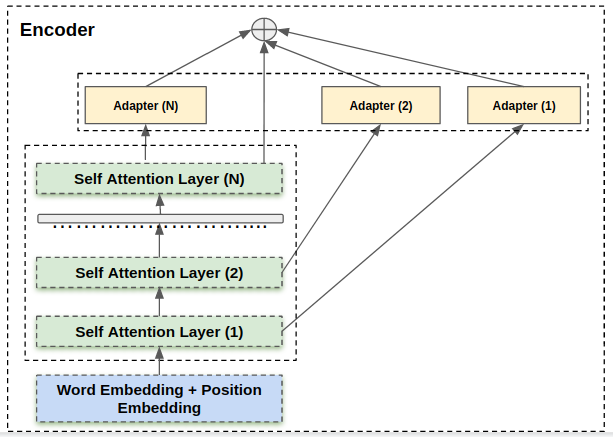
\includegraphics[scale=0.3]{graphics/highway_residual}
  \caption{Highway residual adapter network}
  \label{fig:hrl-architecture}
\end{figure}

\subsection{Gated Residual Adapters \label{ssec:gate}}
\mpDone{Formalizing problem, network design, training algorithm}
The basic architecture presented above rests on a rather simplistic view of ``domains'' as made of well-separated and unrelated pieces of texts that are processed independently during adaptation. Likewise, when translating test documents, one needs to choose between either using one specific domain-adapted model or resorting to the generic model. In this context, using wrong domain labels can have a strong (negative) effect on translation performance. 

Therefore, we would like to design a version of residual adapters that is more robust to such domain errors. This variant, called the \emph{gated residual adapter model}, relies on the training of a supplementary component that will help decide whether to activate, on a word per word basis, a given residual layer and to regulate the strength of this activation. To this end, we extend the highway version of residual adapters as follows.
\fyDone{Consistency of notations wrt section 2.1}

Formally, we replace the adapter computation of equation~\eqref{eq:highway-output} and take the adapted hidden (topmost) layer to be computed as (this is for domain $k$):
\begin{equation}
  \bar{h}^L = h^L + \displaystyle{\mathop{\sum}_{1 \leq i \leq L} \operatorname{ADAP}_k^i(h^i) \odot{} z_k(h^L)}, \label{eq:gated-output}
\end{equation}
where the scalar $z_k(h^L[t]) \in [0,1]$ measures the relatedness of the $t^{\text{th}}$ word $w_t$ to domain $k$. The more likely $w_t$ is in domain $k$, the larger $z_k(h^L[t])$ should be; conversely, for words\footnote{The term ``word'' is employed here by mere convenience, as systems only manipulate sub-lexical BPE units; furthermore, the values of the hidden representations $h^{i}$ at position $t$ depend upon all the other positions in the sentence.} that are not typical of any domain $k$ (eg.\ function words),  adaptation is minimum and the corresponding adapted encoder output ($\bar{h}^L[t]$) will remain close to the output of the generic model ($h^L[t]$). In our implementation, we incorporate two domain classifiers on top of the encoder and the decoder, that take the last hidden layer of the encoder (resp.\ decoder) as input and use the posterior probability $P(k|h^L[t])$ of domain $k$ as the value for $z_k(h^L[t])$.

Training gated residual adapters thus comprises three steps, instead of two for the baseline version:
\begin{enumerate}
\item learn a generic model with mixed corpora from multiple domains.
\item train a domain classifier on top of the encoder and decoder; during this step, the parameters of the generic model are frozen. This model computes the posterior domain probability $P(k|h^L[t])$ for each word $w_t$, based on the representation computed by the last layer.
\item train the parameters of adapters with in-domain data separately for each domain, while freezing all the other parameters.
\end{enumerate}
\fyFuture{is this classifier important, can we train with the rest of the system? Yes we could, but do we want the encoder to be good at classification?}\fyFuture{Check writing to indicate label smoothing for this has been used.}\fyFuture{Can we train a more complex training model ? should we use more monolingual data? etc} 

\section{Experimental settings \label{sec:exp}}

\subsection{Data and metrics \label{ssec:corpora}}
We perform our experiments with two translation pairs involving multiple domains: English-French (En$\rightarrow$Fr) and English-German (En$\rightarrow$De). For the former pair, we use texts\footnote{Most corpora are available from the Opus web site: \url{http://opus.nlpl.eu}} initially from 6~domains, corresponding to the following data sources: the UFAL Medical corpus V1.0 (\domain{med})\footnote{\url{https://ufal.mff.cuni.cz/ufal_medical_corpus}}, the European Central Bank corpus (\domain{bank}) \cite{Tiedemann12parallel}; The JRC-Acquis Communautaire corpus (\domain{law}) \cite{Steinberger06acquis}, documentations for KDE, Ubuntu, GNOME and PHP from Opus collection \cite{Tiedemann09news}, collectively merged in a \domain{it}-domain, Ted Talks (\domain{talk}) \cite{Cettolo12wit}, and the Koran (\domain{rel}). Complementary experiments also use v12 of the News Commentary corpus (\domain{news}). Corpus statistics are in Table~\ref{tab:Corpora-en-fr}.  

\begin{table*}[htbp]
  \centering
  \begin{tabular}{ |lllllll|} %*{4}{|r|}}
    \hline
    %\multicolumn{4}{|l|}{Vocab size - En: 30,165, Fr: 30,398}\\
    \domain{med} & \domain{law} & \domain{bank} & \domain{it} & \domain{talk} & \domain{rel} & \domain{news} \\
    \hline
    2609 (0.68) & 190 (0.05)  & 501 (0.13) & 270 (0.07) & 160 (0.04) & 130 (0.03) & 260 (0) \\
    \hline
  \end{tabular}
\caption{Corpora statistics for En$\rightarrow$Fr : number of parallel lines ($\times 10^3$) and proportion in the basic domain mixture (which does not include the \domain{news} domain). \domain{med} is the largest domain, containing almost 70\% of the sentences, while \domain{rel} is the smallest, with only 3\% of the data.}
\label{tab:Corpora-en-fr}
\end{table*}

En$\rightarrow$De is a much larger task, for which we use corpora distributed for the News task of WMT20\footnote{\url{http://www.statmt.org/wmt20/news.html}} including: European Central Bank corpus (\domain{bank}),  European Economic and Social Committee corpus (\domain{eco}), European Medicines Agency corpus (\domain{med})\footnote{\url{https://tilde-model.s3-eu-west-1.amazonaws.com/Tilde_MODEL_Corpus.html}}, Press Release Database of European Commission corpus, News Commentary v15 corpus, Common Crawl corpus (\domain{news}), Europarl v10 (\domain{gov}), Tilde MODEL - czechtourism (\domain{tour})\footnote{\url{https://tilde-model.s3-eu-west-1.amazonaws.com/Tilde_MODEL_Corpus.html}}, Paracrawl and Wikipedia Matrix (\domain{web}). Statistics are in Table~\ref{tab:Corpora-en-de}.
\begin{table*}[htbp]
  \centering
  \begin{tabular}{ |lllllll|} %*{4}{|r|}}
    \hline
    %\multicolumn{4}{|l|}{Vocab size - En: 30,165, Fr: 30,398}\\
    \domain{bank} & \domain{eco} & \domain{med} & \domain{gov} & \domain{news} & \domain{tour} & \domain{web} \\
    \hline
    4 (0.00022) & 2857 (0.15) & 347 (0.018) & 1828 (0.095) & 3696 (0.19) & 7 (0.00039) & 10473 (0.54) \\
    \hline
  \end{tabular}
\caption{Corpora statistics for En$\rightarrow$De: number of parallel lines ($\times 10^3$) and proportion in the basic domain mixture. \domain{web} is the largest domain, containing about 54\% of the sentences, while \domain{bank} and \domain{tour} are very small.}
\label{tab:Corpora-en-de}
\end{table*}

We randomly select in each corpus a development and a test set of 1,000 lines each and keep the rest for training.\footnote{Scripts to replicate these experiments are available at url{https://github.com/qmpham/experiments.git}.}\fyDone{github} Development sets help choose the best model according to the average BLEU score \cite{Papineni02bleu}.\footnote{We use truecasing and the \texttt{multibleu} script.}\fyDone{A word about meta-parameter settings}\fyDone{Answer question of reviewer 3 about splits ?}
   %    Significance testing is performed using bootstrap resampling \cite{Koehn04statistical}, implemented in compare-mt\footnote{\url{https://github.com/neulab/compare-mt}} \cite{Neubig19compare-mt}. We report significant differences at the level of $p=0.05$.
\fyFuture{Is this part on significance testing still accurate ?}

\subsection{Baseline architectures \label{ssec:baseline}}
Using Transformers \cite{Vaswani17attention} implemented in OpenNMT-tf\footnote{\url{https://github.com/OpenNMT/OpenNMT-tf}} \cite{Klein17opennmt}, we train the following baselines:
\begin{itemize}
\item a generic model trained on a concatenation of all corpora, denoted \system{Mixed};\fyDone{Or mixed nat ?}
\item a fine-tuned model \cite{Luong15stanford,Freitag16fast}, based on the \system{Mixed} system, further trained on each domain with early stopping when the development BLEU score stops increasing during 3 consecutive epochs.
%  We again contrast two versions: full fine-tuning (\system{FT-Full}), which update all the parameters of the initial generic model \system{Mixed}; and the variants of \cite{Bapna19simple} (\system{FT-Block}).
\end{itemize}

For all En$\rightarrow$Fr models, we set the embeddings size and the hidden layers size to~512. Transformers use multi-head attention with 8 heads in each of the 6 layers; the inner feedforward layer contains 2,048 cells. Residual adapters additionally use an adaptation block in each layer, composed of a 2-layer perceptron, with an inner ReLU activation function operating on normalized entries of dimension $b=1024$. \citet{Bapna19simple} showed that the performance of adapted models increases with respect to the size of the inner dimension and obtained performance close to the full fine-tuned model with $b=1024$, which is twice as large as the dimension of a Transformer layer. We used the same setting in our experiments.\fyDone{Check: is it $b$?}

% The gated variant is made of a dense layer, followed by a layer normalization and a sigmoid activation.
% The domain control systems are exactly as their baseline counterparts (RNN and Transformer), with an additional 2 cells encoding the domain on the input layer.
Training uses a batch size of~12,288 tokens; optimization uses Adam with parameters $\beta_1=0.9$, $\beta_2= 0.98$ and Noam decay ($warmup\_steps=4,000$), and a dropout rate of $0.1$ for all layers. For the \system{Mixed} model, we use an initial learning rate of $1.0$ and take the concatenation of the validation sets of 6~domains for development. In the fine-tuning experiments, we continue training using \system{Mixed} as starting point, using the same learning rate schedule, and continuing the incrementation of the number of steps. In the multi-task training, we use the same learning rate schedule as for \system{Mixed}: for each iteration, we sample a domain a probability proportional to its size; we then sample a batch of~12,288 tokens that is used to update the shared parameters and the parameters of the corresponding adapter.\fyDone{Describe the block adaptation layer - voir slides}

Models for En$\rightarrow$De are larger and rely on embeddings as well as hidden layers of size~1024; each Transformers layer contains 16~attention heads; the inner feedforward layer contains 4,096 cells. Adapter modules have the same architecture as for the other language pair, except for their size, which is doubled ($b=2,048$).%\fyTodo{Check: is it $b$?}
%The number of parameters in each model is reported in Table~\ref{tab:params}.

\iffalse{
\begin{table*}[htbp]
  \centering
  \begin{tabular}{|l|l|} \hline
    Model & params \\ \hline 
    \system{Transformer-En-Fr}  & 65 \\
    \system{Residual Adapter-En-Fr} & 1 \\
    \system{Transformer-En-De}  & 213 \\
    \system{Residual Adapter-En-De} & 4 \\
     \hline
  \end{tabular}
  \caption{Number of parameters ($\times 10^6$)}
  \label{tab:params}
\end{table*}
}
\fi

\subsection{Multi-domain systems}
In this section, we evaluate several proposals from the literature on multi-domain adaptation and compare them to full fine-tuning on the one hand, and to two variants of the residual adapter architecture on the other hand.
The reference methods included in our experiments are the following:
\begin{itemize}
\item a system using ``domain control'' \citep{Kobus17domain}. In this approach, domain information is introduced either as an additional token for each source sentence (\system{DC-Tag}) or in the form of a supplementary feature for each word (\system{DC-Feat});
\item a system using lexicalized domain representations \citep{Pham19generic}: word embeddings are composed of a generic and a domain-specific part (\system{LDR});
\item the three proposals of \citet{Britz17effective}. \system{TTM} is a feature-based approach where the domain tag is introduced as an extra word \textsl{on the target side}. The training uses reference tags and inference is performed with predicted tags, just like for regular target words. \system{DM} is a multi-task learner where a domain classifier is trained on top of the MT encoder, so as to make it aware of domain differences; \system{ADM} is the adversarial version of \system{DM}, pushing the encoder towards learning domain-independent source representations. These methods only use domain labels in training.
\end{itemize}

\begin{table*}[t!]
  \centering
  \begin{tabular}{|p{3.5cm}|*{8}{r|}} \hline
%     &&&&&& \\
    Model / Domain & \multicolumn{1}{c|}{\domain{ med}} & \multicolumn{1}{c|}{\domain{ law}} & \multicolumn{1}{c|}{\domain{bank}} & \multicolumn{1}{c|}{\domain{talk}} & \multicolumn{1}{c|}{\domain{ it }} & \multicolumn{1}{c|}{\domain{ rel}} & \multicolumn{1}{c|}{\domain{avg}} \\ \hline 
    \system{Mixed}        & 37.3 & 54.6 & 50.1 & 33.5 & 43.2 & 77.5  &  49.4 \\
    \system{FT-Full}       & 37.7 & 59.2 & 54.5 & 34.0 & 46.8 & 90.8 & 53.8 \\
    \hline 
    \system{DC-Tag}      & 38.1 & 55.3 & 49.9   & 33.2 & 43.5 & 80.5  & 50.1 \\
    \system{DC-Feat}     & 37.7 & 54.9 & 49.5   & 32.9 & 43.6 & 79.9 & 49.9  \\
    \system{LDR}            & 37.0  & 54.7 & 49.9 & 33.9 & 43.6 & 79.9 & 49.8    \\
    \system{TTM}           & 37.3  & 54.9 & 49.5 & 32.9 & 43.6 & 79.9 & 49.7   \\
    \system{DM}            & 35.6  & 49.5  & 45.6 & 29.9 & 37.1 & 62.4 & 43.4   \\ 
    \system{ADM}          & 36.4  & 53.5  & 48.3 & 32.0 & 41.5 & 73.4 & 47.5   \\
    \hline
    \system{Res-Adap}         & 37.3 & 57.9 & 53.9 & 33.8 & 46.7 & 90.2 & 53.3 \\ 
    \system{Res-Adap-MT}  & 37.9 & 56.0 & 51.2  & 33.5 & 44.4 & 88.3 & 51.9 \\
    \system{Res-Adap-MT}$^{+}$ & 37.5 & 57.1 & 52.4 & 33.7 & 46.2 & 89.5 & 52.7 \\
    \hfill {Res-Adap-MT} (gen)    & 37.7 & 51.0 & 34.0 & 30.4 & 34.2 & 15.2 & 36.4 \\
    \hline
  \end{tabular}
  \caption{Translation performance of various multi-domain MT systems (En$\rightarrow$Fr) compared to variants of the residual adapter models.}
  \label{tab:performance-multi}
\end{table*}
The two variants of the residual adapter model included in this first round of experiment have been presented in Section~\ref{ssec:architecture}: \system{Res-Adap} is the multi-domain version of the approach of \citet{Bapna19simple} based on a two-step training procedure; while \system{Res-Adap-MT} is the ``multi-task'' version, where the parameters of the generic model and of the adapters are jointly learned from scratch. We also report results for the same system, using the the parameters of the \system{Mixed} model as initialization (\system{Res-Adap-MT}${^+}$).\footnote{This system also includes a layer dropout policy that cancels adapter layers with probability $0.5$} 

Because of the limit of our computational resources, we restrict the experiments in this section to the En$\rightarrow$Fr task. Results are in Table~\ref{tab:performance-multi}.\fyFuture{Perform experiments for de:en}\fyFuture{Restore results where residual are removed from other paper.}

These results first show that full fine-tuning outperforms all other methods for the in-domain test sets. However, \system{Res-Adap} is able to reduce the gap with this approach for several domains, showing the effectiveness of residual adapters. The ``multi-task'' variant is slightly less effective in our experiments than the basic version, where optimization is performed in two steps. As it turns out, using residual adapters proves here better on average than the other reference multi-domain systems; it is also much better than the generic system for translating data from known domains, outperforming the \system{Mixed} system by more than 4 BLEU points in average. Gains are especially large for small domains such as \domain{law} and \domain{rel}.

% Multi-task training system \system{MDL-Res} gains important improvement compared to baseline \system{Mixed}. However, \system{MDL-Res} is outperformed by \system{Res-Adap}. It means that independently fine tuning the generic models is better than multi-task training. However, \system{MDL-Res} is better than other methods in multi-domain learning including:  \system{DC-Tag},  \system{DC-Feat}, \system{LDR}, \system{TTM}, \system{DM}, \system{ADM}.
Comparing training schemes (\system{Res-Adap} vs \system{Res-Adap-MT} vs \system{Res-Adap-MT}$^+$) suggests that the simultaneous learning of all parameters is detrimental to performance in our settings: we see that the 2-step procedure implemented in \system{Res-Adap} always yields the best scores, even when \system{Res-Adap-MT} is initialized with good parameter values . This may be because in this setting, the adapters have access to a stable version of the generic system. The last line ({Res-Adap-MT} (gen)) gives the results for a \system{Res-Adap-MT} trained system in which we cancel the adapter in inference - comparing this to \system{Mixed} shows how differently the generic parts of these two systems behave.

\subsection{Varying the positions and number of residual adapters}
Tables~\ref{tab:performance-en-fr-pos-reg}-\ref{tab:performance-en-de-pos-reg} report BLEU scores for 6 domains in each language pair: \domain{med},\domain{law},\domain{bank},\domain{talk},\domain{it} and \domain{rel} for En$\rightarrow$Fr; \domain{gov}, \domain{eco}, \domain{tour}, \domain{bank}, \domain{med} and \domain{news} for En$\rightarrow$De. We first see that for the latter direction, the basic version \system{Res-Adap} also outperforms the \system{mixed} baseline on average, with large gains for the small domains \domain{tour}, \domain{bank} and comparable results for the other domains.
% in almost all domains while stays equivalent to the baseline in \domain{med} in En$\rightarrow$Fr and \domain{news}, \domain{gov}, \domain{eco}, \domain{med} in En$\rightarrow$De.
   %    However, \system{FT-full} still remains the best model for all test domains.
\fyFuture{Full FT for en->DE ?}

By varying the number and position of residual adapters (see Section~\ref{ssec:architecture}), we then contrast several implementations. \fyDone{Fix style here} Because the set of possible configurations is large, we only perform experiments for layers $i= 2, 4, 6$ (both for the encoder and decoder). Two settings are considered: keeping just one adapter or keeping the three. The trend is the same for the two language directions: suppressing adapters always hurts the overall performance, albeit by a small margin: having six adapters is better than three, which is better than keeping only one. With only one adapter active, we observe small, insignificant changes in performance when varying the adapter's depth. %\revision{Based on these experiments, it seems that adaptation remains useful even for the deeper layers of the architecture.}\fyFuture{More configurations ?}

\begin{table*}[htbp]
  \centering
  \begin{tabular}{|p{3cm}|*{8}{r|}} \hline
%     &&&&&& \\
    Model / Domain & \multicolumn{1}{c|}{\domain{ med}} & \multicolumn{1}{c|}{\domain{ law}} & \multicolumn{1}{c|}{\domain{bank}} & \multicolumn{1}{c|}{\domain{talk}} & \multicolumn{1}{c|}{\domain{ it }} & \multicolumn{1}{c|}{\domain{ rel}} & \multicolumn{1}{c|}{\domain{avg}} & \multicolumn{1}{c|}{\domain{params}} \\ \hline 
    \system{Mixed}  & 37.3 & 54.6 & 50.1 & 33.5 & 43.2 & 77.5  & 49.4 & 65M/0 \\
    \system{Res-Adap}     & 37.3 & 57.9 & 53.9 & 33.8 & 46.7 & 90.2 & 53.3 & 65M/12M\\ \hline
    \system{Res-Adap$_{(2,4,6)}$}     & 37.7 & 57 & 53 & 33.3 & 45 & 90 & 52.7 & 65M/6M\\
    \system{Res-Adap$_{(6)}$}     & 37.7 & 55.8 & 51.5 & 33.9 & 43.6 & 89.2 & 51.9 & 65M/2M \\
    \system{Res-Adap$_{(4)}$}     & 37.9 & 55.6 & 51.7 & 33.7 & 44.4 & 88.7 & 52 & 65M/2M\\
    \system{Res-Adap$_{(2)}$}     & 37.8 & 55.5 & 51.4 & 34 & 43.8 & 86.7 & 51.5 & 65M/2M\\ \hline
    \system{Res-Adap-WD}     & 37.2 & 56.0 & 52.9 & 33.4 & 46.0 & 90.6 & 52.7 & 65M/12M \\
    \system{Res-Adap-LR}      & 37.4 & 56.1 & 51.8 & 33.3 & 45.0 & 89.7 & 52.2 & 65M/12M \\  
     \hline
  \end{tabular}
  \caption{Translation performance of various fine-tuned systems (En$\rightarrow$Fr). We report BLEU scores for each domain, as well as averages across domains. Column \domain{params} reports the number of domain-agnostic/domain-specific parameters.\label{tab:performance-en-fr-pos-reg}} \fyDone{Boldface ?}
\end{table*}

\begin{table*}[htbp]
  \centering
  \fyDone{Fix column size}
  \begin{tabular}{|p{3cm}|*{8}{r|}} \hline
%     &&&&&& \\
    Model / Domain & \multicolumn{1}{c|}{\domain{ gov}} & \multicolumn{1}{c|}{\domain{ eco}} & \multicolumn{1}{c|}{\domain{tour}} & \multicolumn{1}{c|}{\domain{bank}} & \multicolumn{1}{c|}{\domain{ med}} & \multicolumn{1}{c|}{\domain{news}} & \multicolumn{1}{c|}{\domain{avg}} & \multicolumn{1}{c|}{\domain{params}} \\ \hline
    \system{Mixed}          & 29.3 & 30.5 & 17.6 & 38.1 & 47.9 & 20.9  & 30.6 & 213M/0M\\
   \system{Res-Adap}     & 29.6 & 30.4 & 19.2 & 49.0 & 47.2 & 20.6 & 33.1 & 213M/48M \\ \hline
    \system{Res-Adap$_{(2,4,6)}$} & 29.7  & 30.5 & 18.8 & 49.6 & 47.1 & 20.6 &  32.7 & 213M/24M \\ 
    \system{Res-Adap$_{(6)}$}      & 29.5 & 30.4 & 18.1 & 49.1 & 46.9 & 20.4 & 32.4 & 213M/8M \\
   \system{Res-Adap$_{(4)}$}       & 29.7 & 30.4 & 18.1 & 49.6 & 47.0 & 20.6 & 32.6 & 213M/8M\\
   \system{Res-Adap$_{(2)}$}       & 29.6 & 30.4 & 18.3 & 49.4 & 46.7 & 20.6 & 32.5  & 213M/8M\\
   \hline
    \system{Res-Adap-WD}         & 29.7 & 30.8 & 20.4 & 50.2 & 47.7 & 20.6 & 33.2 & 213M/48M \\
    \system{Res-Adap-LR}           & 29.6 & 30.4 & 19.2 & 49.0 & 47.2 & 20.6 & 33.1  & 213M/48M\\
    \hline
  \end{tabular}
  \caption{Translation performance of various fine-tuned systems (En$\rightarrow$De). We report BLEU scores for each domain, as well as averages across domains. Column \domain{params} reports the number of domain-agnostic/domain-specific parameters.}
  \label{tab:performance-en-de-pos-reg}
\end{table*}

\subsection{Regularizing fine-tuning \label{ssec:regularization-exp}}

The translation from English into German includes two domains (\domain{tour} and \domain{bank}) that are extremely small and account only for a very small fraction of the training data (respectively for 0.039\% and 0.022\% of the total number of sentences). Fine-tuning on these domains can lead to serious overfitting. We assess two well-known regularization techniques for adapter modules, that could help mitigate this problem: weight decay and layer regularization. 

For each method, the optimal hyper-parameter $\lambda$ (weight decay or layer regularization coefficient, see Section~\ref{sssec:design-space}) are chosen by grid search in a small set of values ($\{ 10^{-3}, 10^{-4}, 10^{-5} \}$).\fyFuture{Better grid even better EWC.}

Results in Tables~\ref{tab:performance-en-fr-pos-reg} and \ref{tab:performance-en-de-pos-reg} show that regularizing the adapter model can positively impact the test performance for the smallest domains (this is especially clear for weight-decay (\system{Res-Adap-WD}) in En$\rightarrow$De), at the cost however of a small drop in performance for the other domains. Using layer regularization proves here to be comparatively less effective. Finding better ways to set the regularization parameters, for instance by varying $\lambda$ for each domain based on the available supervision data, is left for future work.  
\fyDone{How is the weight decay parameter set ?}
\fyDone{Why is regularization not helping? It helps for the small domain - domain-specific regularization ??}

\subsection{Highway and Gated Residual Adaptaters \label{ssec:gate-exp}}

We now turn to the evaluation of our new architectural variants: Highway residual adapters \system{Res-Adap-HW} on the one hand, and Gated residual adapters \system{Res-Adap-Gated} on the other hand. We use the same domains and settings as before, focusing here exclusively on the language direction En$\rightarrow$Fr.

To also evaluate the robustness with respect to out-of-domain examples, we perform two additional experiments. We first generate translations with erroneous (more precisely: randomly assigned) domain information: the corresponding results appear in Table~\ref{tab:performance-random} under column \domain{rnd}. We also compute translation for a domain unseen in training (\domain{news}) as follows. For each sentence of this test set, we automatically evaluate the closest domain,\footnote{As measured by the perplexity of a language model trained with only in-domain data.\fyFuture{More on this for reproducibility}.} then use the predicted domain label to compute the translation. This is an error-prone process, which also challenges the robustness of our multi-domain systems. Results are in Table~\ref{tab:performance-random}.
\fyFuture{This is a baseline, and we have not discussed it - keep for next time: We also report model \system{FT-Full-UEW} which is obtained by full-finetuning the generic model using uniform elastic weight to avoid catastrophic forgetting.}

A first observation is that for domains seen in training, our variants \system{Res-Adap-HW} and \system{Res-Adap-Gated} achieve BLEU scores that are on a par to those of the original version (\system{Res-Adap}), with insignificant variations across test sets.\fyFuture{Comment on processing time.}

The two other settings are instructive in several ways: they first clearly illustrate the brittleness of domain-adapted systems, for which large drops in performance (more than 15 BLEU points on average) are observed when the domain label is randomly chosen. Our gated variant however proves much more robust than the other adaptation strategy and performs almost on par to the generic system for that test condition. The same trend holds for the unseen \domain{news} domain, with \system{Res-Adap-Gated} being the best domain adapted system in our set, outperforming the other variants by about 2 BLEU points.
% The phenomenon of Catastrophic Forgetting manifests clearly in this situation where the performance of all multi-domain systems drops dramatically by approximately 10 points BLEU compared to generic model \system{Mixed}. Our proposed model \system{FT-Gate-Block} maintains equivalent performance to the generic model in \system{RND} thanks to the application of adaptive weight on the output of the residual adapter. \system{FT-Gate-Block} avoids relying on the residual adapters when predicting examples that come from domain far from the domain of the adapters. 

% In the new domain test \domain{news}, generic model outperforms other systems. Finetuning systems including \system{FT-Full}, \system{Res-Adap} and \system{FT-HW-Block} underperforms generic model by large margin. More regularized variants including \system{FT-Full-UEW}, and \system{FT-Gate-Block} are able to reduce the gap of performance compared to generic.

% The column \domain{PROC} shows that highway residual adapter \system{FT-HW-Block} process examples faster than the original version \system{Res-Adap}.

% \fyTodo{Why HW worse than standard version ?} 

\begin{table*}[htbp]
  \centering
  \begin{tabular}{|p{3.5cm}|*{7}{r|}|r|r|} \hline
%     &&&&&& \\
    Model / Domain & \multicolumn{1}{c|}{\domain{ med}} & \multicolumn{1}{c|}{\domain{ law}} & \multicolumn{1}{c|}{\domain{bank}} & \multicolumn{1}{c|}{\domain{talk}} & \multicolumn{1}{c|}{\domain{ it }} & \multicolumn{1}{c|}{\domain{ rel}} & \multicolumn{1}{c||}{\domain{avg}} & \multicolumn{1}{c|}{\domain{rnd}} & \multicolumn{1}{c|}{\domain{news}}
\\ \hline %    & \multicolumn{1}{c|}{\domain{PARAMS}}  \\ \hline % & \multicolumn{1}{c|}{\domain{PROC}} \\ \hline  
    \system{Mixed}             & 37.3 & 54.6 & 50.1 & 33.5 & 43.2 & 77.5     &  49.4 & 49.4 & 23.5 \\ %& 65M \\ %& 34s \\ %
    \system{FT-Full}             & 37.7 & 59.2 & 54.5 & 34.0 & 46.8 & 90.8   & 53.8 & 32.5 & 20.2 \\ %& 65M \\ %& 34s \\
    \system{Res-Adap}         & 37.3 & 57.9 & 53.9 & 33.8 & 46.7 & 90.2   & 53.3 & 38.4 & 20.5 \\ %& 65M/12M \\ %& 22s\\ 
    \system{Res-Adap-HW}   & 37.5 & 57.2 & 53.4 & 33.1 & 46.3 & 91.0  & 53.1 & 36.6 & 20.2 \\ %& 65M/12M \\ %& 19s \\
    \system{Res-Adap-HW-MT} & 37.4 & 56.4 & 52.1 & 33.7 & 44.8 & 89.8 & 52.4 & 27.1 & 20.4 \\ %& 65M/12M \\ %&  \\
    \system{Res-Adap-HW-MT}$^{+}$ & 37.7 & 57.0 & 52.5 & 33.5 & 46.1 & 89.0 & 52.6 & 46.5 & 21.4 \\ %& 65M/12M \\ %&  \\
    \system{Res-Adap-Gate}  & 38.0 & 57.5& 53.0 & 33.5 & 46.0 & 90.1  & 53.0 & 49.0 & 22.5 \\ %& 65M/13M \\ %& 21s \\
%    \system{FT-Full-UEW}      & 37.9 & 56.0 & 52.1 & 33.7 & 44.9 & 89.1 &	52.3 & 46.5 & 22.11 \\ %& 34s \\
	\hline
	%\system{Res-Adap-WD} & 37.18 & 55.99 & 52.93 & 33.36 & 46.03 & 90.65 & 52.7 & 38.73 & 20.69 & 65M/12M \\
	%\system{Res-Adap-LR}      & 37.4 & 56.1 & 51.8 & 33.3 & 45.0 & 89.7 & 52.2 &  &  & 65M/12M \\  
    %\hline
  \end{tabular}
  \caption{Translation performance of highway and gated variants for En$\rightarrow$Fr. \domain{news} is excluded from the training data and considered as an out-of-domain test.}
  \label{tab:performance-random}
\end{table*}

\section{Conclusion and outlook \label{sec:discussion}}
\mpDone{discussion}
In this paper, we have performed an experimental study of the residual adapter architecture in the context of multi-domain adaptation, where the goal is to build one single system that (a) performs well for domain seen in training, ideally as well as full fine-tuning; (b) is also able to robustly handle translations for new, unseen domains. We have shown that this architecture allowed us to quickly adapt a model to a specific domain, delivering BLEU performance than are much better than the generic, mixed domain baseline, and close the gap with the full-finetuning approach, at a modest computational cost. Several new variants have been introduced and evaluated for two language directions: if none that able to clearly surpass the baseline, residual adapter models, they provide directions for improving this model in practical settings: unbalanced data condition, noise in label domains, etc. In our future work, we would like to continue the development of the gated variant, which, it seems to us, provides a flexible and robust tool to address the various challenges of multi-domain machine translation.
	\chapter{Dynamic sampling strategies for multi-domain adaptation} \label{chap:mdac}
\section{Introduction}
Building effective Neural Machine Translation models often implies accommodating diverse sets of heterogeneous data so as to optimize performance for the domain(s) of interest. Such multi-source / multi-domain adaptation problems are typically approached through instance selection or reweighting strategies, based on a static assessment of the relevance of training instances with respect to the task at hand. In this work, we study dynamic data selection strategies that are able to automatically re-evaluate the usefulness of data samples and to evolve a data selection policy in the course of training. Based on the results of multiple experiments, we show that such methods constitute a generic framework to automatically and effectively cater to a variety of real-world situations, from supervised multi-domain adaptation to unsupervised domain adaptation. 

As we usually reported in the previous chapters, MDMT train data usually admit an adverse heterogeneity in the domains' data. In the MDMT setting presented in Section ~\ref{ssec:corpora-chap4}, most common MDMT systems hardly achieve significant improvement compared to the generic model. This might prove the brittleness of the MDMT model-centric approaches to the heterogeneity of data. To overcome this challenge, we study the efficacy of the data-centric approaches, and particularly the data sampling methods.

As introduced in Chapter~\ref{chap:mdmt-review}, data sampling approaches aim to find the optimal balance of training data with respect to a certain objective, which can be one or multiple target domains. This is, however, a challenging task due, for instance, to the similarity between domains/languages, but also due to regularization effects of out-of-domain data \citep{Miceli17regularization}. It may also be suboptimal, as some target domains or languages might be easier to train than others. Finally, improving the performance of the MT system in one domain will often hurt that of another \citep{Wees17dynamic, Britz17effective}, and improving model generalization across all domains \citep{koehn18findings} may not achieve optimally for any particular domain. Several recent proposals have explored ways to instead consider \emph{dynamic} data selection and sampling strategies that surpass static strategies. Notably, \citet{Wees17dynamic,Zhang19curriculum} construct a static curriculum, while \citet{Graves17automated,Platanios19competence,Kumar19reinforcement,Wang20learning-multi,Wang20balancing} build curricula that automatically adapt to the training data.

In this chapter, we contribute to this line of research in several ways. First, we propose a novel framework (\emph{Multi-Domain Automated Curriculum}, MDAC for short) that simultaneously accounts for the domain adaptation and the multi-domain adaptation problems. Second, we propose a variant of the work of \cite{Wang20balancing} for building an automated curriculum for training Multi-Domain NMT models. We evaluate our method in various single-domain and multi-domain adaptation settings. We compare our method with several contrasts, including the work of \citet{Zhang19curriculum} and \citet{Wang20balancing}, which was previously only applied to multilingual MT. Based on these experimental results, our main conclusions are that (a) using MDAC often yields overall performance that is as good as the standard fine-tuning strategy for domain adaptation; (b) MDAC can effectively handle a variety of test situations, from targeting one single domain to the full multi-domain scenario. 

\section{Learning with multiple data sources} \label{sec:mdmt-chap7}
First, we want to recall our definition of MDMT setting in Section ~\ref{ssec:formalization-chap4}. Our train instances are distributed according to a mixture $\mathcal{D}_e^S$ such that $\mathcal{D}_e^S(x) = \sum_{d=1}^{n_d} \lambda^{s}(d) \mathcal{D}^d_e(x)$, with $\{\lambda^{s}(d), d=1 \dots n_d\}$ the mixture weights satisfying $\sum_d \lambda^{s}(d)=1$. In the sequel, we also use boldface to denote the vector $\vlambda$, and $\lambda(d)$ is used to denote a scalar corresponding to the $d^{th}$ element of the vector $\vlambda$.

The main challenge is then to make the best of this heterogeneous data, with the aim to achieve the optimal performance for the intended test conditions. These might correspond to data from just one of the training domains, as in standard supervised (multi-source) domain adaptation; a more difficult case is when the test data is from one domain unseen in training (unsupervised domain adaptation); in multi-domain adaptation finally, the test distribution is itself a mixture of domains, some of which may also be observed in training.  Without loss of generality, one may then assume that the test distribution takes the form $\mathcal{D}^{T}_e(x) = \sum_{d=1}^{n_d} \lambda^{t}(d) \mathcal{D}_e^d(x)$ - with only one non-null  component in the case of pure domain adaptation. These settings are illustrated on Figure~\ref{fig:mdmt-lambdas-chap7}.
\begin{figure}[h]
  \centering
  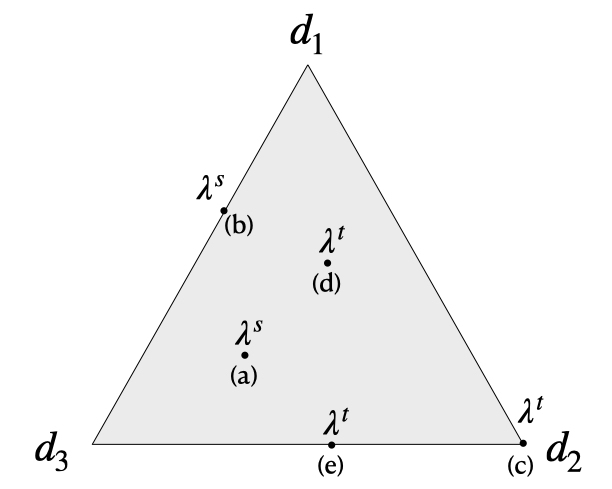
\includegraphics[width=0.48\textwidth]{graphics/mdmt-lambdas}
  \caption{Training and testing with distribution mismatch. We consider just three domains, and represent vectors of mixture weights $\vlambda^{s}$ and $\vlambda^{t}$ in the 3-dimensional simplex. Training with weights in (a) and testing with weights in (c) is supervised multi-source domain adaptation to domain~2 ($d_2$), while (b)-(c) is the unsupervised version, with no training data from $d_2$; training with weights in (a) and testing with weights in (d) is multi-domain learning, also illustrated with configurations (a)-(e) (training domain $d_1$ is not seen in test), and (b)-(d)  (test domain $d_2$ is unseen in training).}\label{fig:mdmt-lambdas-chap7}
\end{figure}

These situations have been amply documented from a theoretical perspective (eg.\ \citet{Mansour09multiple,Mansour09domain,Hoffman18algorithms}). A general recommendation in the DA setting is to adjust the sampling distribution used to optimize the system so as to compensate for the mismatch between $\mathcal{D}_e^S(x)$ and $\mathcal{D}_e^T(x)$. This can be approximated by reweighting instances, or more conveniently domains, which are selected during training with a probability $\lambda^{l}(d)$, with $\lambda^{l}(d) \neq \lambda^{s}(d)$.

A widely used approach to supervised DA is \emph{fine-tuning} \citep{Luong15stanford,Freitag16fast}, where $\vlambda^{l}$ is allowed to vary during learning. With our notations, this approach amounts to first learning an initial parameter value with all the data ($\forall d, \lambda^{l}(d) = \lambda^{s}(d)$), then to continue training with only batches from the test domain $d_t$ ($\lambda^{l}(d) = \indic{d = d_t}$) with $\indic{A}$ the indicator function for predicate $A$. Note that this strategy is potentially suboptimal, as some out-of-domain samples may contribute to the final performance due to eg.\ domain overlap. Optimizing the learning distribution in multi-domain settings is even more challenging, as the learner has to best take advantage of potential domains overlaps, and also of the fact that some domains might be easier to learn than others.

\section{Multi-Domain Automated Curriculum } \label{sec:mdac-chap7}
\subsection{Basic principles}
Assuming training data in each of the $n_d$ domains $d_1 \dots d_{n_d}$, we denote the size of the training corpus from domain $d$ as $N^{s}_d$, and $N^{s} = \sum_d N^{s}_d$ is the total number of training samples. We use $\widehat{\mathcal{D}^{d,l}_e}$ and $\widehat{\mathcal{D}^{d,t}_e}$ to denote the empirical train and test distributions for domain $d$ over the source language $e$, and $\widehat{\mathcal{D}^u_e}(x;\vlambda^{u}) = \sum_{d} \lambda^{u}(d) \widehat{\mathcal{D}^{d,u}_e}(x)$ for $u\in\{l,t\}$. In our setting,  $\vlambda^t$, and hence $\widehat{\mathcal{D}^t_e}(x;\vlambda^t)$ are fixed and predefined, approximated with an equivalent number of development corpora. 

% Our method
MDAC constructs an adaptative training distribution $\vlambda^{l}$ that optimizes the data selection policy along with the training of the NMT model. We parameterize $\vlambda^{l}$ by a differentiable function $\vlambda^l(\vpsi)$. We divide the training into many short sessions; in each session $t$, the model is trained with a static data distribution $\vlambda^{l}(\vpsi_t)$. After one learning session, we update the data distribution using the REINFORCE algorithm of \citet{Williams92simple}. The evolution of $\vpsi$ is thus defined by:
\begin{align*}
\vpsi_{t+1} &= \vpsi_t + \mathbf{lr}_{1} * \displaystyle{\mathop{\sum}_{d=1}^{n_d}} R(d) * \frac{\partial \lambda^l(d;\vpsi_t)}{\partial \vpsi}, \\
\end{align*}
\begingroup
\allowdisplaybreaks
where reward $R(d)$ is computed as:
\begin{align*}
  R(d) = J^t(\theta_t,\vlambda^t) - J^t(\theta_{t+k},\vlambda^t),
\end{align*}
and where we also define:
\begin{equation}
\begin{array}{rcl}
\theta_{t+i} &=& Update\big(\theta_{t+i-1},[x^i_j,y^i_j]_{j=1}^N\big) \\ \nonumber
 i \in \{ 1,\cdots,k \}
x^i_j &\sim& \widehat{D^{d,l}_e}(x), y^i_j \sim g^d(x^i_j) \\
J^t(\theta,\vlambda_t) &=& \displaystyle{\mathop{\sum}_{d=1}^{n_d}}\lambda^t(d)\displaystyle{\mathop{\sum}_{x^{d,t} \sim \widehat{D^{d,t}_e},y^{d,t} \sim g^d(x^{d,t})}} l(\theta,x^{d,t},y^{d,t}).
\end{array}
\end{equation}
\endgroup
In these equations, $k$ is number of simulation step, $N$ denotes the size of a batch; $\mathbf{lr}_{1}$ is the learning rate of the sampling distribution; $l(\theta,x,y) = -\displaystyle{\mathop{\sum}_{i}^{l_y}}log P(y_i|y_{<i},x;\theta)$ is the loss of the NMT model on sample $(x,y)$; $J^t(\theta,\vlambda_t)$ is the weighted loss aggregated over $n_d$ dev-sets corresponding to the $n_d$ domains.

To compute the reward $R(d)$ of using data from domain $d$ to train the model, we simulate $k$ training steps from the current checkpoint by training the model with $k$ batches sampled from $D^l(d)$ and compute the gain of the weighted dev-loss. This computation is inspired by the target prediction gain in \citet{Graves17automated}. However, where \citet{Graves17automated} used accumulated gains from the past as rewards, we instead predict the usefulness of each domain for improving the future performance of the system given its current state. This is achieved by simulating a round of training with only the data from one domain. Furthermore, the choice of the parameterization of the sampling distribution in our method differs from that of \citet{Graves17automated}, although this choice is empirical.

The work of \citet{Wang20balancing} is also related: it is based on the Bi-level Optimization framework, which aims to find an optimal static distribution $\vlambda^{l}$ that will result in the best NMT model with respect to a given target dev set at the end of training. These authors also derive a similar form of update for $\vpsi$. However, their reward is the cosine similarity between the gradient computed with the training data from one domain and the gradient computed with the dev set. We compare this approach with ours in the experiment section.

\subsection{MDAC for (multi) domain adaptation}
The setting developed in previous sections is quite general and can, in principle, accommodate the variety of situations mentioned above, and many more: basic domain adaption, multi-domain adaptation with various target distributions, possibly including domains unseen in training. In our experiments, we would like to better assess the true potential of MDAC in these settings and seek to experimentally answer the following questions:
\begin{itemize}
\item is MDAC a viable alternative to conventional fine-tuning? In particular, does it enable to better take advantage of relevant data from other domains?
\item is MDAC also a viable option in multi-domain adaptation scenarios?
\item does MDAC also enable to perform \emph{unsupervised} (multi-)domain adaptation? \fyDone{TBContinued}
\end{itemize}
These questions are further explored in section~\ref{sec:results-chap7}. We now turn to our experimental conditions.

\section{Experimental settings} \label{sec:exp-chap7}
\subsection{Data and metrics \label{ssec:corpora-chap7}}
In this work, we reuse the MDMT setting of Section ~\ref{ssec:corpora-chap4}, which has proved to be challenging for MDMT systems. We uses the same metric and processing procedure as in Section ~\ref{ssec:corpora-chap4}. For the sake of brevity, we will not provide the description here.

\subsection{Baseline systems \label{ssec:baseline-chap7}}
Our baselines are standard for multi-domain systems.\footnote{We however omit domain-specific systems trained only with the corresponding subset of the data, which are always inferior to the mix-domain strategy \citep{Britz17effective}.} Using Transformers \citep{Vaswani17attention} implemented in OpenNMT-tf\footnote{\url{https://github.com/OpenNMT/OpenNMT-tf}} \citep{Klein17opennmt}, we build the following systems:

\begin{itemize}
\itemsep0em 
\item Generic models trained with predefined mixtures of the training data taking the form:
\begin{align} \label{mixture:trn-chap7}
\lambda_{\alpha}(d) = \frac{q_d^{\alpha}}{\displaystyle{\mathop{\sum}_{d=1}^{n_d}q_d^{\alpha}}} &&
q_d = \frac{\mid N^{s}_d \mid}{\displaystyle{N^{s}}} % \mathop{\sum}_{i=1}^K\mid D_i \mid}}
\end{align}
with $\alpha \in \{0,0.25,0.5,0.75,1.0\}$. We denote these as \system{Mixed-$\alpha$} below. \system{Mixed-$0$} uses a uniform distribution, \system{Mixed-$1.0$} the empirical domain distribution;
\item fine-tuned models \citep{Luong15stanford,Freitag16fast} which was already presented in Section ~\ref{ssec:baselines-chap4}. Their implementations are provided in Appendix ~\ref{appendix:a};
\item systems trained with fixed data mixtures corresponding to $\vlambda^l \in \big[ \vlambda_0, \vlambda_{0.25}, \vlambda_{0.5}, \vlambda_{0.75}, \vlambda_{1.0}\big]$; these are used in the multi-domain experiments of Section~\ref{ssec:mda-chap7};
\item  our own implementations of recent dynamic sampling proposals from the literature: Curriculum Learning (CL) of \citet{Zhang19curriculum} and Differential Data Selection (DDS) of \citet{Wang20balancing} (see details below);
\end{itemize}

All models use embeddings and hidden layers of dimension~512. Transformer models contain 8~attention heads in each of the 6+6 layers; the inner feedforward layer contains 2048 cells. Training lasts for 200K iterations, with batches of~12,288 tokens, Adam with parameters $\beta_1=0.9$, $\beta_2= 0.98$, Noam decay ($warmup\_steps=4000$), and a dropout rate of $0.1$ in all layers.

\subsection{CL and DDS's re-implementation}\fyDone{Right place for this ?}
We re-implement DDS in Tensorflow without any change in the choices of parameterization and hyper-parameters compared to the original code of \citet{Wang20balancing}.\footnote{\url{https://github.com/cindyxinyiwang/multiDDS}}
% 
We also re-implement the approach of \citet{Zhang19curriculum} according to the authors' description. For each domain adaptation experiment, we combine the training data of all other domains into one corpus then compute the cross-entropy difference score of each source sentence of this combined dataset. We then sort and split the corpus into 9 shards and execute curriculum learning with 10 shards, using the in-domain corpus as the first shard.

\subsection{MDAC systems} \label{ssec:dds-sys-chap7}
The behavior of MDAC only depends on (a) the initial domain distribution at the start of training $\vlambda^{l}_{t=0}$, and (b) the targeted (dev/test) distribution $\vlambda^{t}$. We thus report these systems as \system{MDAC($\vlambda^{l}_{t=0}$, $\vlambda^{t}$)} and compare with DDS using the same settings.

In our work, we parameterize the distribution $\vlambda^l$ as follows (with $\beta=2$\footnote{This setting corresponds to the \emph{spherical softmax} of \cite{Brebisson16anexploration}.} in all experiments):\fyDone{Explain why}
\begin{equation}
\lambda^l(d;\vpsi) = \frac{\psi[d]^\beta}{\sum_i \psi[i]^\beta}. \nonumber
\end{equation}
This parameterization avoids the ``rich-get-richer'' effect that we observe when using $\vlambda(\vpsi) = \operatorname{softmax}(\vpsi)$, which yields gradients wrt. $\psi[d]$ that are proportional to $\exp(\psi[d])$ (see also Figure~\ref{fig:sampling-chap7}). Additional settings for the hyper-parameters of our method include the number of simulation steps $k=10$ and the learning rate $\mathbf{lr}_{data}=0.001$. We update the sampling distribution via 100 gradient descent iterations for almost all experimental settings except that for adaptation with automatic clusters (Section~\ref{ssec:clda-chap7}), where we use 20~gradient descent iterations to avoid converging to degenerate distributions.\fyFuture{Why? computation?} We split the training into 100 short sessions that last 2000 training steps each. The choice of those hyper-parameters is mostly heuristic except for the learning rate $\mathbf{lr}_{data}$ which is optimized via grid search over a set of values $\{0.001,0.0025,0.005\}$.

The computational cost of our approach is due to the simulation step, which is conducted after every 2000 iterations to compute the reward of each domain. During the simulation step, we update the temporary checkpoint with $k$ updates for each domain, which cost as much as $k$ training updates. Therefore, we execute $k \times n_d$ updates in total after every 2000 iterations. Our algorithm approximately costs $1 + \frac{k \times n_d}{2000}$ times as much as a standard training.

\subsection{Experimental tasks}
We evaluate and compare our method with multiple baselines in the 5 following conditions.
%including: domain adaptation; multi-domain adaptation, bi-domain adaptation, unseen domain adaptation, and unsupervised domain adaptation.
In the \emph{supervised domain adaptation task}, given the data from 6 domains (\domain{med}, \domain{bank}, \domain{law}, \domain{it}, \domain{talk}, \domain{rel}), we aim to build distinct expert NMT models for each domain. To challenge the flexibility of the method, we also consider a \emph{bi-domain adaptation task}, where given the same 6 domains, we only focus on adapating only to 2 domains.

In the \emph{multi-domain adaptation task}, given the same 6 domains, we aim to build one single NMT model that would perform optimally, assuming a uniform distribution of domains during the test.

In a fourth experiment (\emph{unseen domain adaptation}), given training data in 6 domains and a small development set of a new domain (\domain{News} in our case), we aim to build an NMT model which performs well for the unseen domain.

Finally, in the \emph{unsupervised domain adaptation task}, we cluster all available training data into 30~clusters using the KNN algorithm in the same way as in \citep{Tars18multidomain}, then adapt these clusters to one of 6 domains using the corresponding in-domain dev set. We compare MDAC to DDS for each of our 6 test sets.

\section{Results and discussion \label{sec:results-chap7}}
\subsection{Domain Adaptation}\label{ssec:da-chap7}
In this setting, we aim to build an NMT model for one single domain: we accordingly set $\vlambda^t$ to a deterministic distribution $\vlambda_d$, where the target domain $d$ has probability~1.

We consider three initializations for MDAC and DDS, using $\vlambda_0$, $\vlambda_1$ and $\vlambda_d$. According to Table~\ref{tab:da-chap7}, MDAC achieves the overall best performance when $\vlambda_{t=0} = \vlambda_0$.  Doing so proves much better than initializing with $\vlambda_d$ for small domains: \domain{talk}, \domain{bank} and\domain{it}. Conversely, initializing with $\vlambda_d$ is beneficial when targeting large domains such as \domain{med} and \domain{law}. The same conclusion holds for DDS. 

We now compare the best MDAC system (using $\vlambda_{t=0} = \vlambda_0$) to full fine-tuning. According to Table~\ref{tab:da-chap7}, fine-tuning is better for large domains such as \domain{med} and \domain{law}, while MDAC outperforms fine-tuning by approximately 1.2 BLEU for \domain{bank} and 1.0 BLEU for \domain{rel}. This indicates that for small domains, out-of-domain data helps improve the generalization and that MDAC is able to exploit both the in-domain and the out-of-domain training data instead of edging out the out-of-domain training data as in fine-tuning. Results for DDS display similar trends but are always outperformed by MDAC. The behavior of CL, which does only well the large domain \domain{med} lag somewhat behind.

\begin{table*}[htbp]
  \centering \small
  \begin{tabular}{|l|*8{r|}} \hline
    domain \hfill $d=$ & \multicolumn{1}{c|}{\domain{ med}} & \multicolumn{1}{c|}{\domain{ law}} & \multicolumn{1}{c|}{\domain{bank}} & \multicolumn{1}{c|}{\domain{talk}} & \multicolumn{1}{c|}{\domain{ it }} & \multicolumn{1}{c|}{\domain{ rel}} & \multicolumn{1}{c|}{avg.} \\ \hline
    FT-Full($d$) &40.3&63.8&54.4&38.5&52.0&91.0&56.7\\ \hline
    \hline
    \system{CL($d$)} &40.2&60.2&53.7&36.5&51.1&91.1&55.5\\ \hline
    \system{DDS($\vlambda_0, \vlambda_d$)} &39.6&60.1&55.0&38.5&52.5&92.0&56.3\\
    \system{MDAC($\vlambda_0, \vlambda_d$)} &39.6&62.5$^{**}$&55.6$^{*}$&38.5&52.4&92$^{***}$&56.8\\
     \hline
    \system{DDS($\vlambda_1, \vlambda_d$)} &39.7&53.9&49.6&37.9&43.1&64.3&48.1\\
    \system{MDAC($\vlambda_1, \vlambda_d$)} &40.2&59.9&52.6&38.5&50.7&79.8&53.6\\ \hline
    \system{DDS($\vlambda_d, \vlambda_d$)} &39.9&63.9&54.5&35.4&51.2&91.8&56.1\\
    \system{MDAC($\vlambda_d, \vlambda_d$)}&40.6&63.9&54.5&35.6&51.3&92.3&56.4\\
    \hline
  \end{tabular}
  \caption{Domain adaptation experiments. We report BLEU scores of each method for 6 target domains and their average: each column corresponds to a distinct system. ($^{*}$) MDAC is significantly better than CL, fine-tuning and DDS with $p<0.05$. ($^{**}$) MDAC is significantly better than CL and DDS with $p<0.05$. ($^{***}$) MDAC is significantly better than CL, fine-tuning with $p<0.05$.}
  \label{tab:da-chap7}
\end{table*}

\subsection{Bi-domain adaptation}\label{ssec:bida-chap7}

In these control experiments, we showcase the flexibility of dynamic sampling and try to adapt to (arbitrary) pairs of target domains with equal weight and contrast our results with those of DDS. Results are in Table~\ref{tab:bi-da-chap7}. Here, MDAC significantly outperforms DDS in two settings (\domain{med+it} and \domain{law+bank}) while being surpassed in \domain{talk+rel}.
% Allthough we showing that MDAC is capable to adapt to a variable set of target domains.

\subsection{Multi-domain adaptation}\label{ssec:mda-chap7}

We now turn to a more realistic scenario and consider multi-domain adaptation, which aims to train one single system with optimal performance averaged over 6 domains. This setting targets a uniform test distribution $\vlambda^t = \vlambda_0$. In this situation, CL \citep{Zhang19curriculum} does not apply. We therefore only contrast the performance of MDAC, DDS and several fixed training data distribution $\vlambda^l \in \big[ \vlambda_0, \vlambda_{0.25}, \vlambda_{0.5}, \vlambda_{0.75}, \vlambda_{1.0}\big]$, where $\vlambda_{\alpha}$ is defined according to equation~\eqref{mixture:trn-chap7}.

We again initialize MDAC and DDS with two distribution $\vlambda_0$ and $\vlambda_1$. According to Table~\ref{tab:multi-da-chap7}, MDAC achieves the best performance with initial (uniform) $\vlambda_0$. The same conclusion holds for DDS. For this configuration, MDAC outperforms in average static training distributions including $\big[ \vlambda_0, \vlambda_{0.75}, \vlambda_{1.0}\big]$ by a significant margin, and performs slightly better than $\big[ \vlambda_{0.25}, \vlambda_{0.5} \big]$. This indicates that MDAC allows us to skip the somewhat heuristic choice of the optimal training mixture.

A second observation is that DDS is again outperformed by MDAC by a significant margin of 1.5 BLEU on average; the only domain where DDS does (much) better is \domain{med}. Figure~\ref{fig:sampling-chap7}, where we plot the evolution of the training mixture in the course of training sessions, helps understand the difference between the two methods. For DDS (Figure~\ref{fig:DDS-chap7}), the sampling distribution quickly converges towards a bi-domain mode in which only \domain{med} and \domain{rel} have significant probability -- hence the good performance on the former domain. In contrast, the distribution computed by MDAC evolves more smoothly; small domains such as \domain{bank}, \domain{it}, \domain{talk} and \domain{rel} receive a larger proportion of training data in the early stages; their weights then slowly decrease as larger domains such as \domain{med} and \domain{law} increase their share. This, however, only happens at the end of the training, when the NMT models might have already been close to their optimal performance for the small domains.

\begin{table*}[htbp]
  \centering \small
  \begin{tabular}{|l|*7{r|}} \hline
    domain \hfill $d=$ & \multicolumn{1}{c|}{\domain{ med}} & \multicolumn{1}{c|}{\domain{ law}} & \multicolumn{1}{c|}{\domain{bank}} & \multicolumn{1}{c|}{\domain{talk}} & \multicolumn{1}{c|}{\domain{ it }} & \multicolumn{1}{c|}{\domain{ rel}} \\ \hline \hline
    \system{DDS($\vlambda_0, \vlambda_2$)}&39.5&-&-&-&50.1&- \\
    \system{MDAC($\vlambda_0, \vlambda_2$)}&39.1&-&-&-&51.8$^*$&- \\
    \system{DDS($\vlambda_0, \vlambda_2$)}&-&60.8&53.3&-&-&- \\
    \system{MDAC($\vlambda_0, \vlambda_2$)}&-&61.9$^*$&54.5$^*$&-&-&- \\
    \system{DDS($\vlambda_0, \vlambda_2$)}&-&-&-&37.9&-&91.3 \\ 
    \system{MDAC($\vlambda_0, \vlambda_2$)}&-&-&-&36.9&-&90.4 \\
    \hline
  \end{tabular}
  \caption{Adapting to two domains. For a given line, non empty columns correspond to the pair of target domains. ($^*$) MDAC is significantly better than DDS with $p<0.05$.}
  \label{tab:bi-da-chap7}
\end{table*}

\begin{table*}[htbp]
  \centering \small
  \begin{tabular}{|l|*8{r|}} \hline
    domain \hfill $d=$ & \multicolumn{1}{c|}{\domain{ med}} & \multicolumn{1}{c|}{\domain{ law}} & \multicolumn{1}{c|}{\domain{bank}} & \multicolumn{1}{c|}{\domain{talk}} & \multicolumn{1}{c|}{\domain{ it }} & \multicolumn{1}{c|}{\domain{ rel}} & \multicolumn{1}{c|}{mean} \\ \hline \hline
    % Multidomain
    \system{Mixed-0} &38.6&59.3&53.7&37.3&51.0&90.4&55.1\\
    \system{Mixed-0.25}&38.9&59.6&53.3&37.6&50.5&90.6&55.1\\
    \system{Mixed-0.5}&39.0&60.2&52.5&38.5&51.9&90.3&55.4\\
    \system{Mixed-0.75}&39.4&59.9&51.9&38.8&50.0&87.6&54.6\\
    \system{Mixed-1}&40.3&59.5&49.8&36.4&49.0&80.0&52.5\\
    \hline \hline
    \system{DDS($\vlambda_0, \vlambda_0$)} &40.1&56.9&50.7&37.4&46.8&92.0&54.0\\ 
    \system{MDAC($\vlambda_0, \vlambda_0$)}&38.5&60.3$^{**}$&54.4$^*$&37.3&51.3$^{**}$&91.4$^*$&55.5$^{**}$\\ 
    \hline \hline
    \system{DDS($\vlambda_1, \vlambda_0$)} &40.6&55.5&48.0&36.2&46.9&60.1&47.9\\
    \system{MDAC($\vlambda_1, \vlambda_0$)}&40.2&59.3$^{**}$&51.0$^{**}$&36.9$^{**}$&48.6$^{**}$&80.7$^{**}$&52.8$^{**}$\\
    \hline
  \end{tabular}
  \caption{Multi domain adaptation. For a given line, all the columns \emph{correspond to the same multi-domain system}. ($^*$) MDAC is significantly better than \system{Mixed-$\alpha$} with $p<0.05$. ($^{**}$) MDAC is significantly better than DDS with $p<0.05$.}
  \label{tab:multi-da-chap7}
\end{table*}

\begin{figure*}[htbp]
\begin{subfigure}{.5\textwidth}
  \centering
  % include first image
  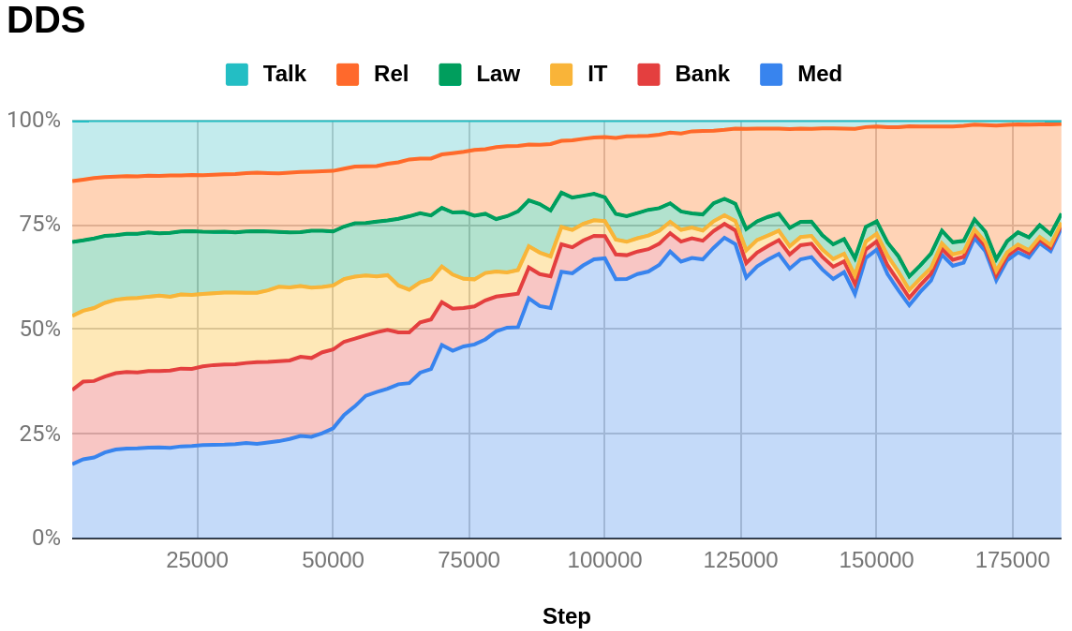
\includegraphics[width=0.97\textwidth]{graphics/DDS.png}  
  \caption{DDS}
  \label{fig:DDS-chap7}
\end{subfigure}
\begin{subfigure}{.5\textwidth}
  \centering
  % include second image
  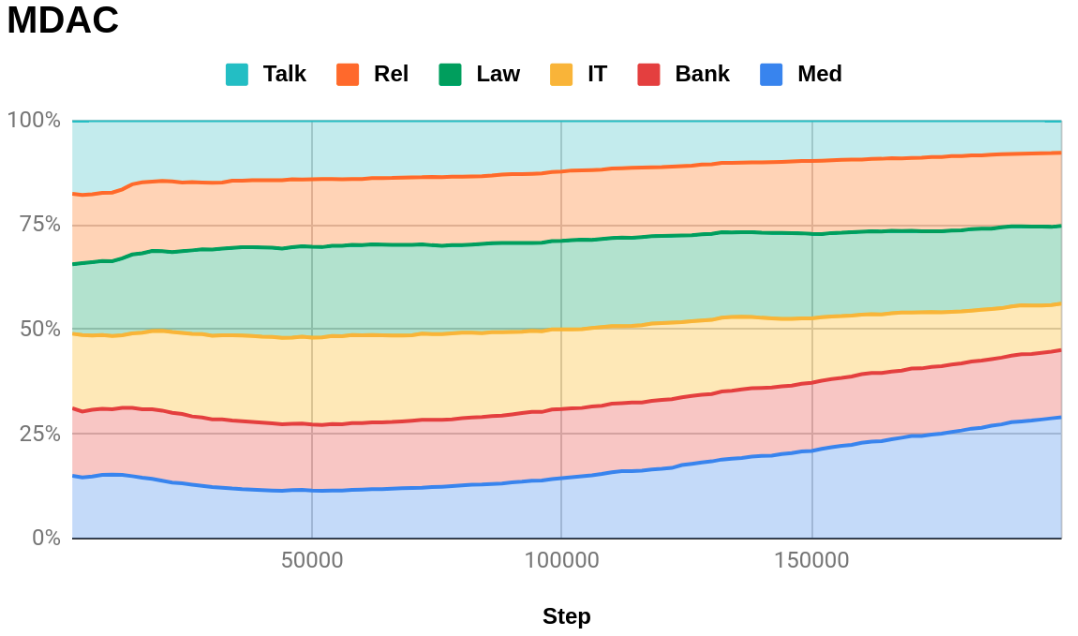
\includegraphics[width=0.97\textwidth]{graphics/MDAC.png}  
  \caption{MDAC}
  \label{fig:MDAC-chap7}
\end{subfigure}
\caption{Evolution of the sampling distribution during training.}
\label{fig:sampling-chap7}
\end{figure*}

\begin{table*}[htbp]
  \centering \small
  \begin{tabular}{|l|*{10}{r|}} \cline{1-2} \cline{4-11}
    domain \hfill $d=$ & \multicolumn{1}{c|}{\domain{news}}& \hfill &domain \hfill $d=$ & \multicolumn{1}{c|}{\domain{ med}} & \multicolumn{1}{c|}{\domain{ law}} & \multicolumn{1}{c|}{\domain{bank}} & \multicolumn{1}{c|}{\domain{talk}} & \multicolumn{1}{c|}{\domain{ it }} & \multicolumn{1}{c|}{\domain{ rel}} & \multicolumn{1}{c|}{mean}  \\ 
\cline{1-2} \cline{4-11}
    \multicolumn{2}{|c|}{\sl Unseen domain} & &\multicolumn{8}{c|}{\sl Training with 30 clusters} \\ 
\cline{1-2} \cline{4-11}
    \system{Mixed-0}      & 25.7 & &\system{DDS($\vlambda^*, \vlambda_d$)}&38.3&60.1&50.3&35.8&49.1&90.1&53.9\\
    \system{Mixed-0.25} & 25.8 & &\system{MDAC($\vlambda^*, \vlambda_d$)}&39.2$^*$&61.6$^*$&52.0$^*$&38.2$^*$&49.1&89.7&55.0$^*$\\ \cline{4-11}
    \system{Mixed-0.5}   &26.5\\
    \system{Mixed-0.75} &26.8\\
    \system{Mixed-1} &26.9 \\
    \cline{1-2}
     \system{DDS($\vlambda_0, \vlambda_{news}$)} &26.3 \\
     \system{MDAC($\vlambda_0, \vlambda_{news}$)} &26.3 \\
     \cline{1-2}
  \end{tabular}
  \caption{Unseen domain adaptation (left) and unsupervised adaptation (right). For a given line, each column corresponds to one distinct system. ($^*$) MDAC is significantly better than DDS.}
  \label{tab:unsupervised-da-chap7}
\end{table*}

\subsection{Unseen domain}\label{ssec:uda-chap7}
The left part of Table~\ref{tab:unsupervised-da-chap7} displays the performance on the unseen domain \domain{news} for NMT systems trained with the mixtures $\vlambda^l \in \big[ \vlambda_0, \vlambda_{0.25}, \vlambda_{0.5}, \vlambda_{0.75}, \vlambda_{1.0}\big]$ and with dynamic data selection (MDAC and DDS). These systems have insignificant differences in BLEU, showing that dynamic mixture does not improve the robustness of the NMT system against unseen domains. However, the fact that the performance of MDAC and DDS is close to the best performance is a sign that they can also apply in such challenging situations. % the robustness of the NMT model.

\subsection{Automatic clustering}\label{ssec:clda-chap7}
The right part of Table~\ref{tab:unsupervised-da-chap7} reports the performance of NMT systems adapted to each domain.\footnote{A more detailed analysis is in the supplementary material.} In comparison to Section~\ref{ssec:da-chap7}, the training data is distributed in 30 automatic clusters instead of the 6 original domains. Splitting the train data into small groups provides the learner with extra degrees of freedom when selecting the best distribution. However, as these clusters are built automatically, they are noisier in nature. According to the results in Table~\ref{tab:unsupervised-da-chap7}, this scenario is hard both for DDS and MDAC, which perform much worse than for the supervised DA setting. This again signals the importance of initialization: analyzing the clustering, we find that the data for \domain{rel} mostly correspond to one single cluster. When using a uniform initialization, this cluster starts with a very small weight and never succeeds in yielding the (good) performance observed in the DA setting.

\subsection{Reward analysis}

\begin{figure*}[htbp]
\begin{subfigure}{.5\textwidth}
  \centering
  % include first image
  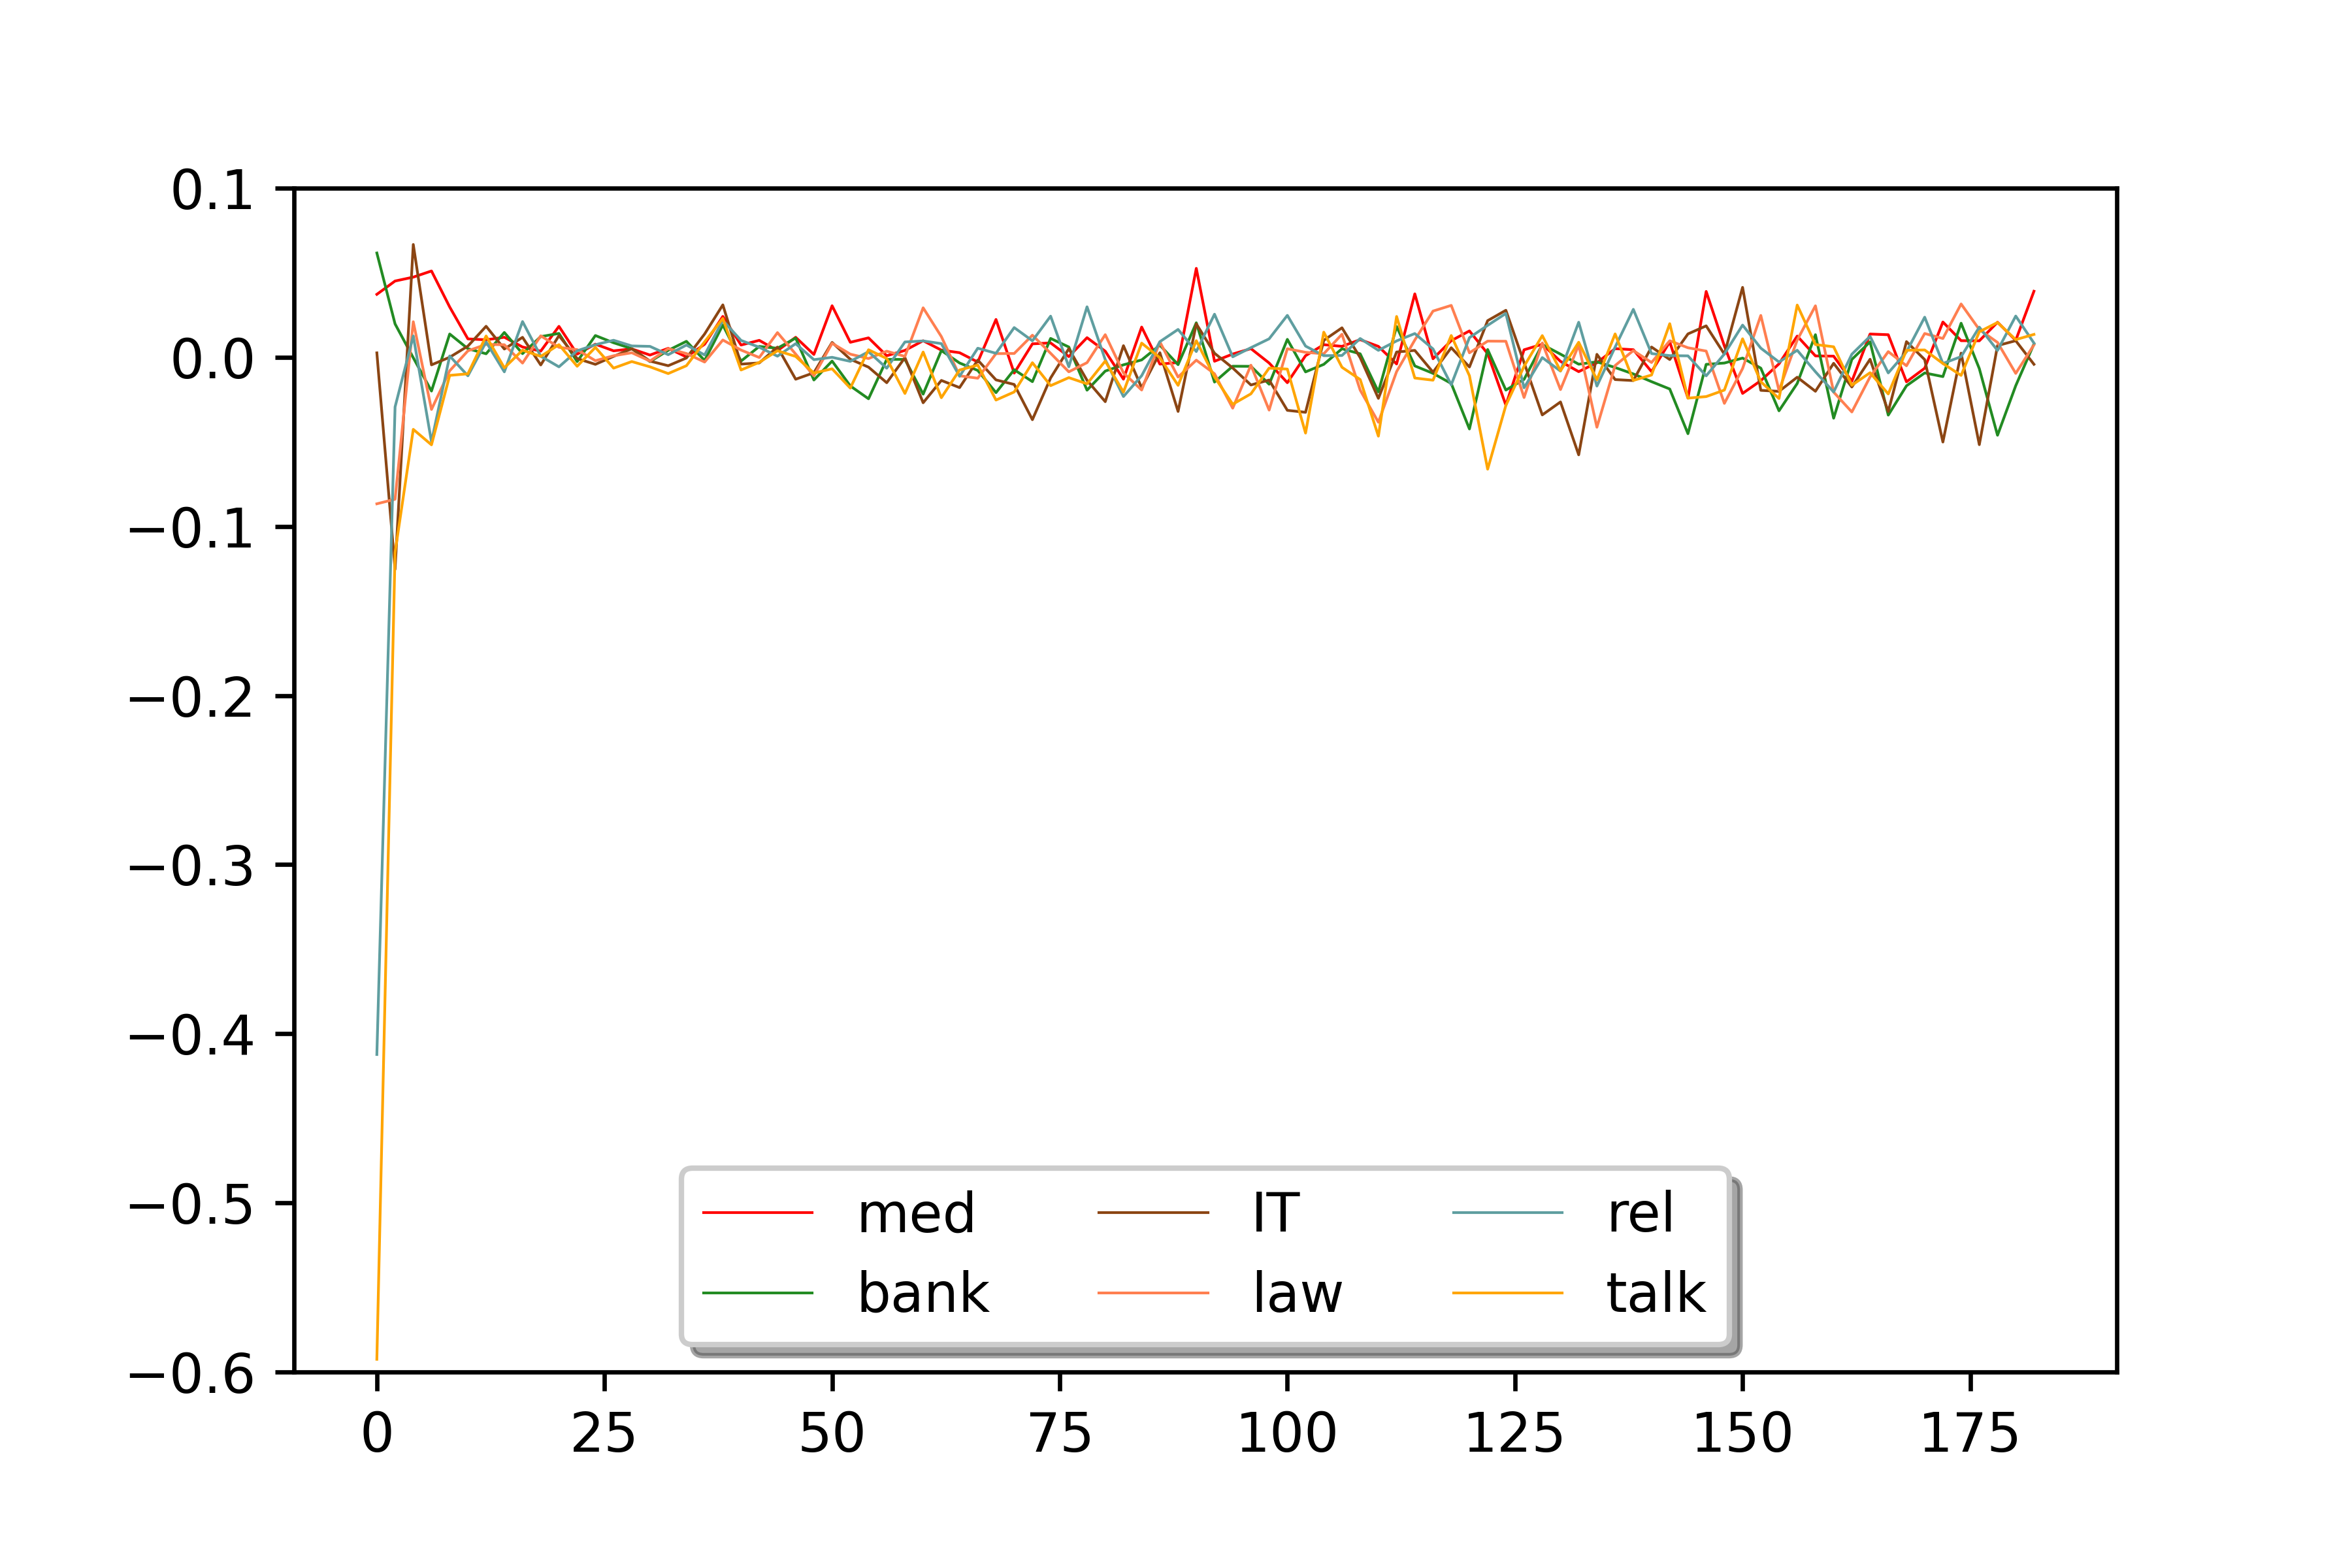
\includegraphics[width=0.97\textwidth]{graphics/rewards_dds.png}  
  \caption{DDS}
  \label{fig:reward-dds-chap7}
\end{subfigure}
\begin{subfigure}{.5\textwidth}
  \centering
  % include second image
  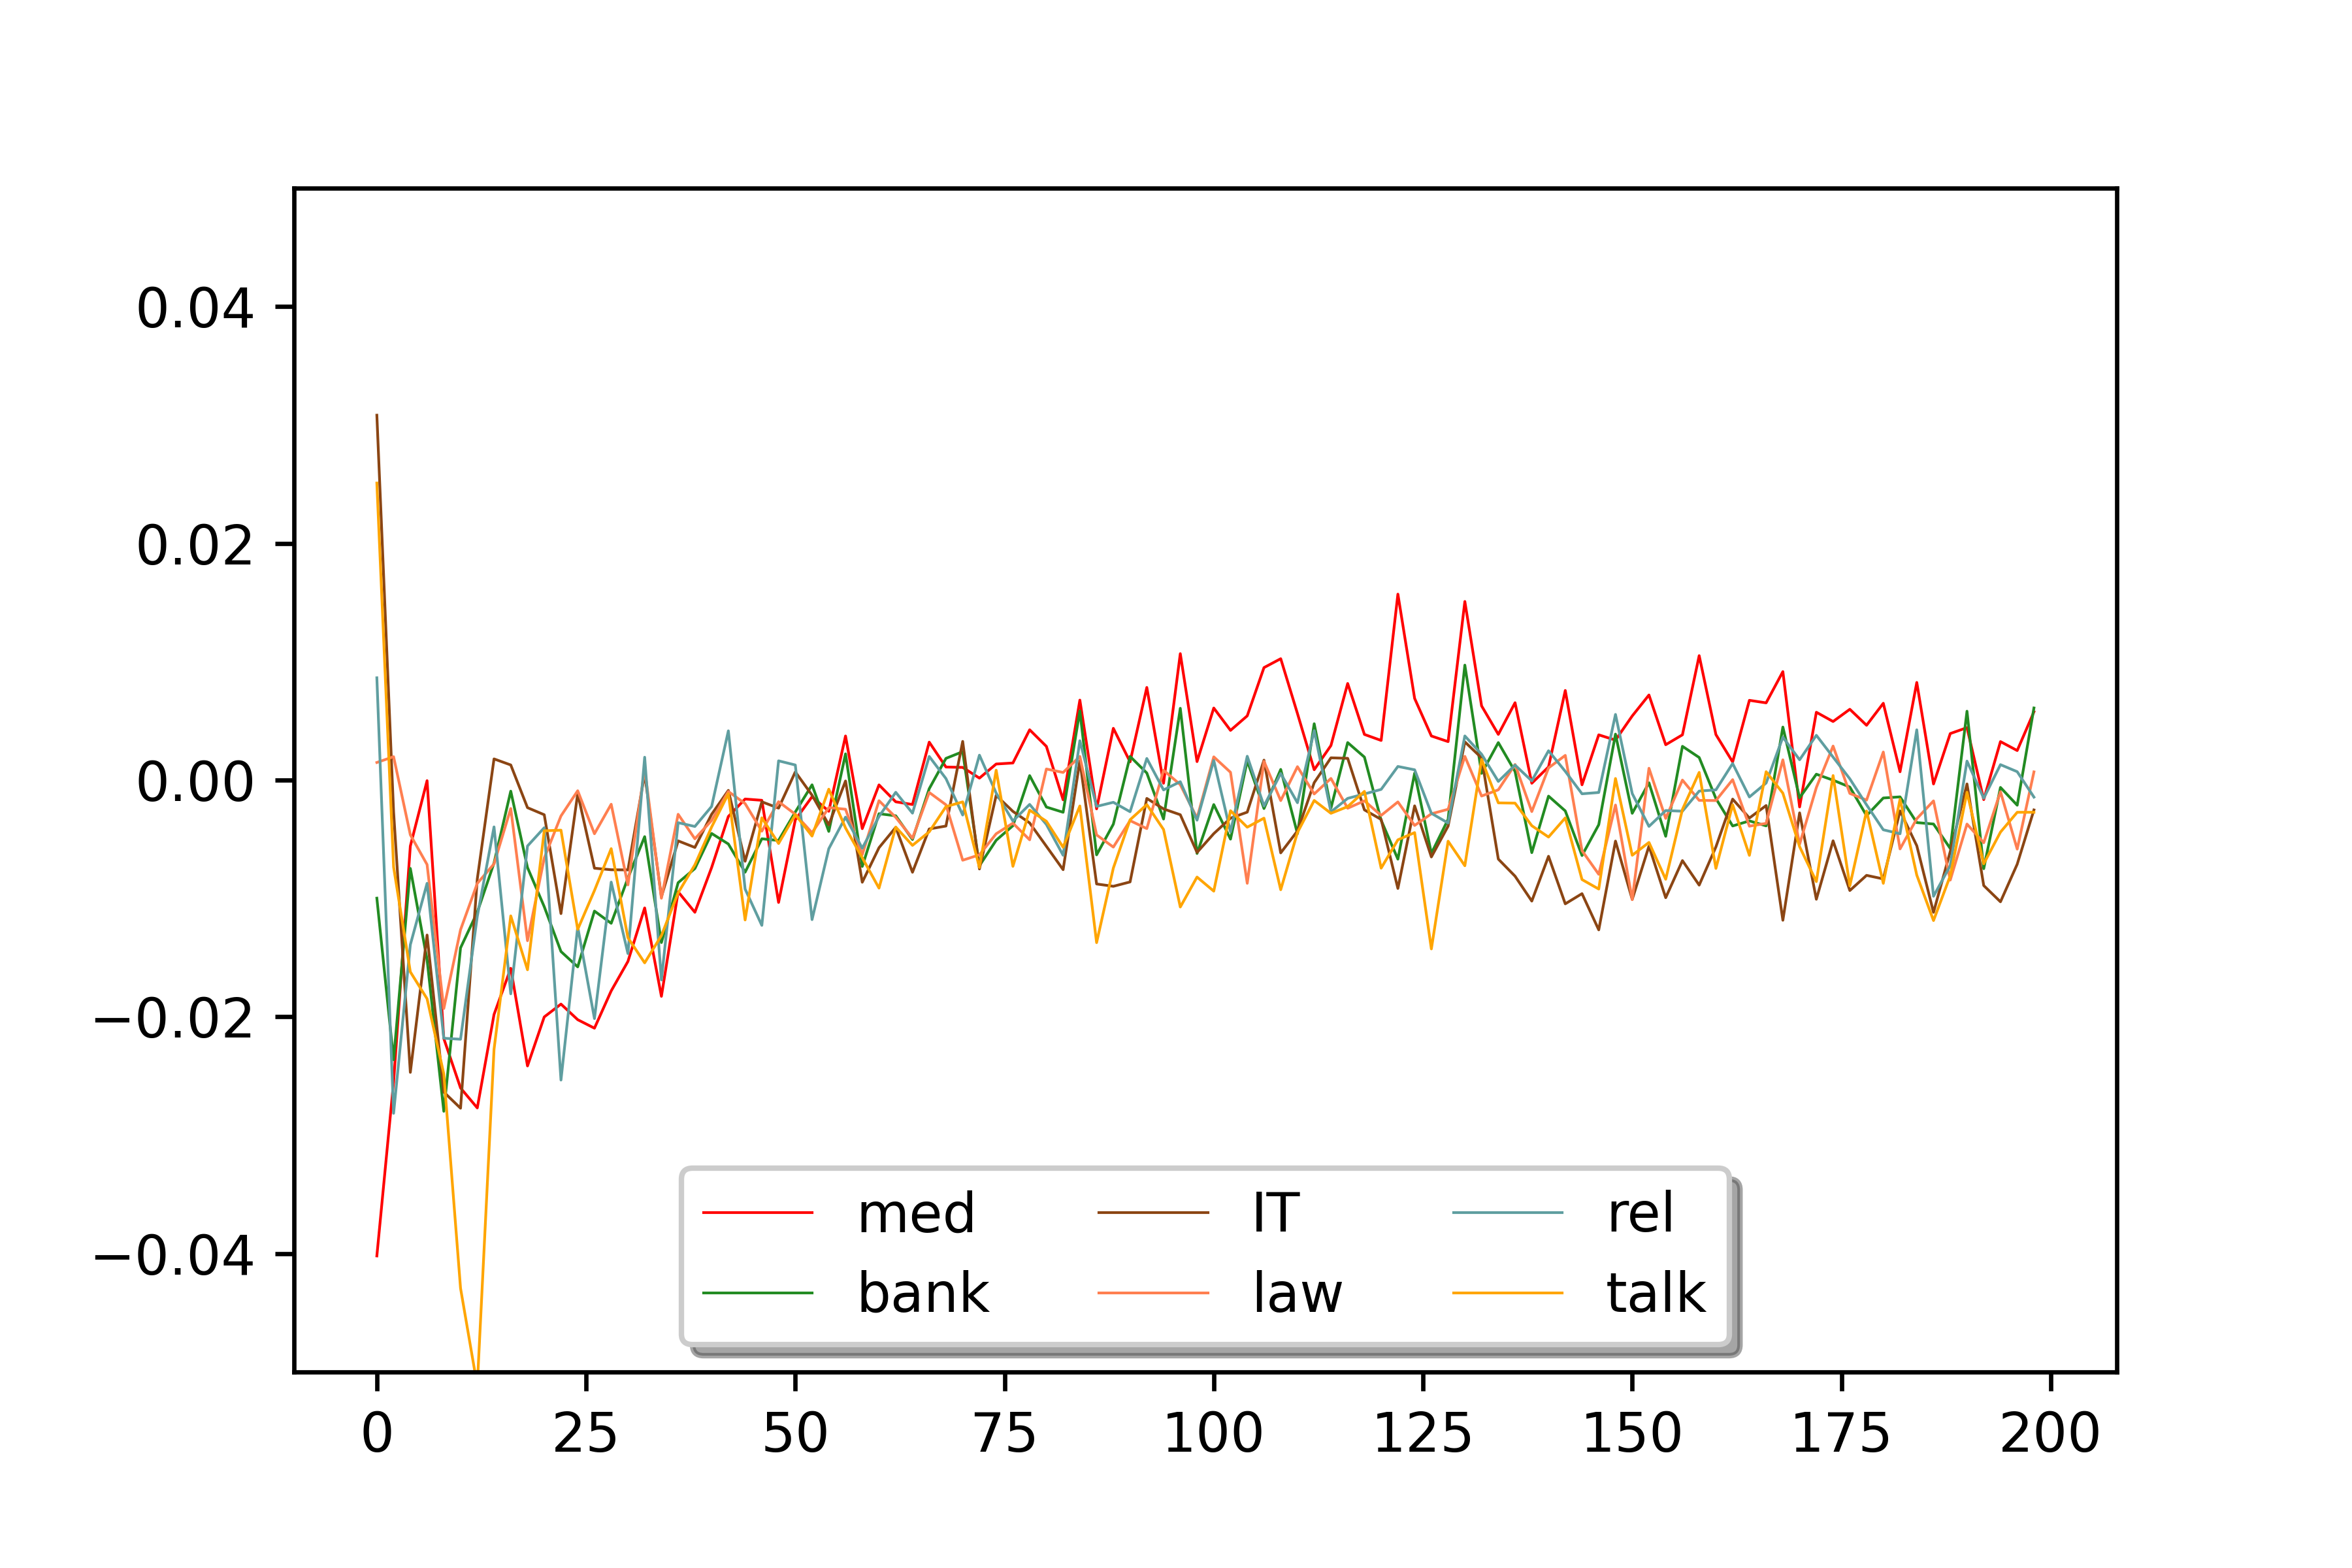
\includegraphics[width=0.97\textwidth]{graphics/rewards_loss.png}  
  \caption{MDAC}
  \label{fig:reward-loss-chap7}
\end{subfigure}
\caption{Evolution of the rewards during training.}
\label{fig:reward-chap7}
\end{figure*}

For MDAC, the magnitude of the rewards decreases dramatically from $1.e\text{-}2$ to $1.e\text{-}3$ in about first 10k iterations, then stays around $1.e\text{-}3$ until the end of the training. We have not tried to rescale the magnitude of rewards to $(\text{-}1,1)$ as proposed in \citet{Graves17automated} but left this perspective for the future work. 

For DDS, the magnitude of the rewards decreases dramatically from $1.e\text{-}1$ to $1.e\text{-}2$ in about first 10k iterations, then stays around $1.e\text{-}2$ until the end of the training.


\section{Related Work \label{sec:related-chap7}}

Most approaches to adaptive/dynamic data selection take inspiration from \citet{Bengio09curriculum}, where the notion of curriculum learning is introduced. CL relies on the notion of the ``easiness'' of a sample to schedule the presentation of training data so that the easiest examples are presented first and the hardest last. Various ways to automate CL using the framework of multi-armed bandits are explored in \citep{Graves17automated}, which has been an inspiration for our implementation. While the initial aim was primarily to improve and speed up training, CL has also proven useful for domain adaptive / multi-domain / multilingual MT, based on alternative definitions of ``easiness''.\fyDone{Ajouter Grave}
For instance, \citet{Zhang19curriculum} study supervised DA and propose a curriculum approach which progressively augments the training data: in the early stages, only in-data is used, while shards containing less relevant\footnote{Domain distance is computed with Lewis-Moore scores (based on the cross-entropy of in-domain LM and mixed-domain LM).} data are introduced in later stages. This is somehow opposite to the recommendations of \citet{Wees17dynamic}, whose \emph{gradual fine-tuning} progressively focuses on the in-domain data.

\citet{Kumar19reinforcement} use reinforcement techniques (deep Q-learning) to learn the curriculum strategy: in this work, complexity corresponds to difficulty levels which are binned using contrastive data selection. The reward is based on the decrease of the development set's loss that results from the actual data selection strategy.\fyDone{Alert: what do we do during warm-up ?} The same technique is recently applied to multilingual NMT in \citep{Kumar21learning}. \citet{Zhou20uncertainty} propose another curriculum-based approach which instead relies on \emph{instance uncertainty} as a measure of their difficulty and presents the data sample starting with the easiest (more predictable) first. Another contribution of this work is an alternative criterium for stopping the training. More related to our problems, \citet{Wang20learning-multi} adapt CL for multi-domain adaptation, where an optimal instance weighting scheme is found using Bayesian optimization techniques. Each step consists of (a) weighting instances based on relevance features, (b) fine-tuning a pretrained model using the weighted training set, and is applied iteratively to train a sequence of models. The one that maximizes the development set performance is finally retained.

\section{Conclusion and outlook}

In this study, we have presented a generic framework to perform a variety of standard adaptation tasks for machine translation, ranging from the conventional supervised domain adaptation to multi-domain adaptation and unseen domain adaptation. By experimenting with all these settings, we have shown that the same algorithm, aimed at automatically finding an effective data sampling scheme during the course of training, could be used in all these situations. This algorithm, we believe, provides us with a more sound approach to (multi-domain) DA than existing heuristics and dispenses with the costly search of optimal meta-parameters. Another contribution of our work is an experimental comparison of recent approaches to dynamic data selection. In the future, we intend to continue developing this approach and improve its effectiveness. One issue that we have left unaddressed is reward normalization. We remarked that rewards in early stages of the training have much higher magnitude than in the middle and ending stages making pre-mature judgments of the utility of each domain. \citet{Kumar19reinforcement} also reported this problem. \citet{Graves17automated} proposed a simple rule for re-scaling rewards to the interval $(-1,1)$. Another area where we need to progress is the unsupervised learning setting of Section~\ref{ssec:clda-chap7}, where our results still lag way behind that of supervised DA - this might be due to the inability of our simplistic optimization strategy to handle a large number of domains.
	\chapter{Attempts at unsupervised multi-domain adaptation}
\label{chap:priming}
\section{Introduction}
In this chapter, we discuss recent studies on the fourth setting of MDMT presented in Section \ref{sec:case4}. When the test domain is undetermined, we can work around by adapting the generic NMT system to a latent domain of the test sentence on the fly. \citet{Li18onesentence, Farajian17multidomain} used similar sentences to adapt the NMT system to the test sentence. The authors proposed finetuning the NMT model over a batch of similar sentences retrieved from a translation memory (TM\nomenclature[tm]{TM}{Translation memory}). We group these method under "one-sentence adaptation paradigm". Recent works of ~\citet{bulte19neural,xu20boosting} introduced a simple and elegant framework where similar translations are used to improve the context of the translation effectively boosting translation accuracy. We group these methods into the group of "context-augmented NMT". In all cases, context-augmented NMT is performed by simply injecting retrieved sentences in the input stream prior to inference decoding. Context-augmented NMT and one-sentence adaptation can be grouped into a larger category, that we name retrieval-based MT.

In this chapter, our primary goal is to compare two paradigms: on-the-fly one-sentence adaptation \citep{Farajian17multidomain,Li18onesentence} and augmented context NMT \citep{bulte19neural,xu20boosting}. We also discuss how different retrieval methods affect the quality of context-augmented NMT. 

Finally, we propose a variant of \citet{bulte19neural}, which performs slightly better and can be used with monolingual data, providing a scenario where NMT can be effectively helped by large amounts of available data. Our proposal does not require to change the NMT architectures or algorithms, relying solely on input preprocessing and on prefix (forced) decoding \citep{rebecca16neural,santy19inmt}, a feature already implemented in many NMT toolkits.

\section{Context-augmented NMT}
\label{sec:priming-chap8}
This section describes the general context-augmented NMT with similar translations. We follow the work by ~\citet{bulte19neural,xu20boosting} and build a translation model that incorporates similar translations from a translation memory (TM) to boost translation accuracy. In this work, TMs are parallel corpora containing translations falling in the same domain as test sentences.

The following section describes several common retrieval methods used in \citet{Farajian17multidomain,bapna19non,bulte19neural,xu20boosting}. We will also describe a variant of \citet{pagliardini18unsupervised}, which is developed by Josep Maria Crego.
\subsection{Similarity Computation}
\label{ssec:sim-chap8}
We detail the sentence similarity tools evaluated in this work. The first employs discrete word representations\fyDone{As opposed to? why not discrete / continuous}, while the rest relies on building distributed representations of sentences to perform similar sentence retrieval:
\paragraph{\system{FM}:} fuzzy matching is a lexicalized matching method aimed to identify non-exact matches of a given sentence. Following~\citet{xu20boosting}, we use \texttt{FuzzyMatch}\footnote{\url{https://github.com/systran/FuzzyMatch}}, where the fuzzy match score $\operatorname{FM} (s_i,s_j)$ between two sentences $s_i$ and $s_j$ is:
    \begin{equation*}
    \operatorname{FM} (s_i,s_j) = 1 - \frac{\operatorname{ED} (s_i,s_j)}{max(|s_i|,|s_j|)}
    \label{eq:FM-chap8}
    \end{equation*}
    \noindent with $\operatorname{ED}(s_i,s_j)$ being the Edit Distance between $s_i$ and $s_j$, and $|s|$ is the length of $s$. 
\paragraph{\system{S2V}:} we use \texttt{sent2vec}\footnote{\url{https://github.com/epfml/sent2vec}}~\citep{pagliardini18unsupervised} to generate sentence embeddings. The network implements a simple but efficient unsupervised objective to train distributed representations for sentences. The model is based on efficient matrix factor (bilinear) models~\citep{Mikolov13efficient,Mikolov13distributed,Pennington14glove}.
%Borrowing the notations of~\citet{pagliardini18unsupervised}, training the model is formalized as an optimization problem:
%
%\begin{equation*}
%\min_{\vect{U},\vect{V}} \sum_{s\in \mathcal{C}} f_{s} (\vect{UV}\iota_{s})
%\end{equation*}
%\noindent 
%for two parameter matrices $\vect{U} \in \R^{|\mathcal{V}|\times d}$ and $\vect{V} \in \R ^{d\times |\mathcal{V}|}$, where $\mathcal{V}$ denotes the vocabulary and $d$ is the embedding dimension, $\iota_{s}$ is a binary vector encoding the bigrams in $s$ (bag of bigrams encoding). The minimization of the cost function $f_{s}$ is performed on a training corpus $\mathcal{C}$ of sentences $s$.
%In \texttt{sent2vec},
\paragraph{\system{CBON}:} the Continuous Bag of $n$-grams (\texttt{CBON}) 
 model denotes our re-implementation of the previous \texttt{sent2vec} model. In addition to multiple implementation details, the main difference is the use of arbitrary large $n$-grams to model sentence representations, where \texttt{sent2vec} only used bigrams.

\vspace{0.1cm}

Both \texttt{sent2vec} and \texttt{CBON} learn a source (or context) embedding $\vect{v}_w$ for each $n$-gram $w$ in the vocabulary $\mathcal{V}$.
Once the model is trained, the embedding of sentence $s$ ($h_s$) is obtained as the average of its $n$-gram embeddings:

\begin{equation*}
    \vect{h}_s = \frac{1}{|R(s)|} \sum_{w\in R(s)} \vect{v}_w
\end{equation*}

\noindent where $R(s)$ is the list of $n$-grams (including unigrams) occuring in sentence $s$ and $\vect{v}_w$ is the target embedding of $n$-gram $w$.

The similarity score $\operatorname{EM} (s_i,s_j)$ between two sentences $s_i$ and $s_j$ is then defined via the cosine similarity of their sentence vector representations $h_i$ and $h_j$:\fyDone{$h$ is earlier a dimension ?}
\begin{equation*}
\operatorname{EM} (s_i, s_j) = \frac{h_i \cdot h_j}{||h_i|| \times ||h_j||},
\label{eq:EM-chap8}
\end{equation*}
\noindent where $||h||$ denotes the norm of vector $h$.

Note that models differ in their vocabularies, which are built selecting the most frequent $n$-grams.
Both models implement Negative Sampling to avoid the softmax computation. 

\subsection{How to present similar translations to an NMT model}
\label{ssec:schemes-chap8}
There are several schema to integrate similar translations to an NMT model. We describe below three simple schema, which do not require change in the NMT architecture.

\paragraph{\system{tgt$^k$}} this approach was proposed in the work of~\citet{bulte19neural},
where the input sentence in the source language is augmented with the $k$ translations (in the target language) having the highest matching score ($\operatorname{FM}$ or $\operatorname{EM}$) in the TM. 

In training, sentence pairs ($\textbf{s}$,$\textbf{t}$) are preprocessed as follows: the source sentence $\textbf{s}$ is concatenated with translations $t^k$ of the $k$ most similar sentences ($s^k$) to $\textbf{s}$ found in the TM. Augmented translations are sorted by matching score, with $k=1$ denoting the most similar. Sentences in the source stream are separated using the special token $\circ$.

\begin{center}
%\begin{tabular}{r|l}
\begin{tabular}{ll}
\texttt{src:} & $t^{k} \circ ... \circ t^{2} \circ t^{1} \circ \textbf{s}$ \\
\texttt{tgt:} & $\textbf{t}$%  \\
\end{tabular}
\end{center}
\noindent In inference, only the source-side is input to the translation network.

\citet{xu20boosting} reported an issue in the method of \citet{bulte19neural} regarding {\em unrelated} tokens present in similar translations $t^k$. The model effectively learns to copy most of the content present in similar translations, but has difficulties to avoid also copying {\em unrelated} words. Consider for instance the input sentence $s=$ {\it pertussis vaccin} with similar sentence $s^1=$ {\it measles vaccin} and its corresponding translation $t^1=$ {\it vaccin contre la rougeole}. Following the \system{tgt$^k$} scheme, the NMT input consists of:
\begin{center}
\begin{tabular}{c}
\it vaccin contre la rougeole $\circ$ {\bf pertussis vaccin} \\
\end{tabular}
\end{center}
\noindent yielding the output: {\bf vaccin contre la rougeole}.
%
The word {\it rougeole} is actually the translation of an unrelated word ({\it measles}). The model often copies such {\em unrelated} tokens~\citep{xu20boosting}, due to the fact that they are present in the input stream as similar translations ($t^k$) and are usually semantically related to the correct translation choice (here {\it coqueluche}, the correct translation for {\it pertussis}).

\paragraph{\system{tgt$^k$+STU}} adopts the proposal of~\citet{xu20boosting} to alleviate the {\em unrelated word} problem. It relies on an additional source stream (factor) to label related/unrelated tokens. In this scheme the input of the NMT model contains two parallel streams:\fyDone{A tag for the sep symbol?}

\begin{center}
\scalebox{0.88}{
\begin{tabular}{p{0.05\textwidth}p{0.045\textwidth}p{0.04\textwidth}p{0.005\textwidth}p{0.055\textwidth}p{0.002\textwidth}p{0.075\textwidth}l}
\setlength\tabcolsep{0.0pt}
\texttt{src$_1$:} & vaccin & contre & la & rugeole & $\circ$ & \bf pertussis & \bf vaccin \\
\texttt{src$_2$:} & T & T & T & U & T & S & S \\
\texttt{$\,\,\,$tgt:} & vaccin & contre & la & coqueluche \\
\end{tabular}
}
\end{center}

Tokens in the second stream are: S for source tokens, U for unrelated and T for related target tokens.\fyDone{R for Unrelated ?} {\it rougeole} is thus tagged as an {\it unrelated} word that must not be copied in the translation output.
Word embeddings are built after concatenating both factor embeddings.
%
\citet{xu20boosting} claim achieving a 8\% reduction of unrelated tokens when using this scheme.

Note that this solution is computationally expensive as it requires to identify related/unrelated tokens in each input sentence and in the corresponding similar translations, based in \citet{xu20boosting} on word alignments and edit distance computations.

\paragraph{\system{s+t$^k$}} the solution introduced in \citet{Pham20Priming} relieves us from the tagging burden. It considers both sides of similar translations ($s^k$ and $t^k$). Training streams take the form:

\begin{center}
\begin{tabular}{rl}
\texttt{src:} & $s^{k} \circ ... \circ s^{2} \circ s^{1} \circ \textbf{s}$ \\
\texttt{tgt:} & $\textcolor{black}{t^{k} \circ ... \circ t^{2} \circ t^{1} \circ}\ \textbf{t}$ \\
\end{tabular}
\end{center}
\noindent In inference, target-side similar translations \textcolor{black}{$t^k$} are used by the model as a target prefix. The initial steps of the beam search use the given prefix $\textcolor{black}{t^{k} \circ ... \circ t^{2} \circ t^{1} \circ}$ in forced decoding mode, returning to a regular beam search after the last \textcolor{black}{$\circ$} token is generated.

A similar strategy of concatenating previous and current sentences was explored by \citet{tiedemann17neural} in the context of handling discourse phenomena.
However, since we use true translation as prefixes, our strategy does not suffer from exposure bias~\cite{Ranzato15sequence} and the subsequent error propagation problem.
%
Continuing on our running example, during inference the model receives:
\begin{center}
\begin{tabular}{rl}
\texttt{input:} & \it measles vaccin $\circ$ {\bf pertussis vaccin} \\ 
\texttt{prefix:} & \it \textcolor{black}{vaccin contre la rougeole $\circ$} \\
\end{tabular}
\end{center}
\noindent the encoder embeds the input stream, and force-decodes the target prefix,  before starting the translation generation. Note that during beam search, the decoder has thus access both to all input tokens ($s^k$ and $s$) as well as to similar translations \textcolor{black}{$t^k$} (in the translation prefix). 
\section{Experimental Framework}
\label{sec:eperiments-chap8}

\subsection{Corpora}
\label{ssec:corpora-chap8}
In this chapter, we use an experimental setting larger than the one of Chapter~\ref{chap:revisiting}. We experiment with the English-French language pair and data originating from eight domains, corresponding to texts from three European institutions: 
the European Parliament (\domain{EPPS}), 
the European Medicines Agency (\domain{EMEA}) and
the European Central Bank (\domain{ECB});
Legislative texts of the European Union (\domain{JRC});
IT-domain corpora corresponding to \domain{KDE4} and \domain{GNOME};
News Commentaries (\domain{NEWS});
and parallel sentences extracted from Wikipedia (\domain{WIKI}).
%
Table~\ref{tab:corpora-chap8} contains statistics regarding the corpora used in this work\footnote{Freely available from~\url{http://opus.nlpl.eu}}~\citep{Tiedemann12parallel}. Statistics are computed after splitting off punctuations.

\begin{table}[!ht]
\begin{center}
\scalebox{0.83}{
\begin{tabular}{l | r | r r | r r }
\hline
%\vspace{-0.15cm}
\multirow{2}{*}{Corpus} & \multirow{2}{*}{\#Sents (K)} & \multicolumn{2}{c|}{L$_{mean}$} &  \multicolumn{2}{c}{Vocab (K)} \\
 &  & \small English & \small French & \small English & \small French \\
\hline
\multicolumn{6}{c}{\textit{Parallel Corpora}} \\
\hline
\domain{EPPS}      & 1,992.8 & 27.7 & 32.0 & 129.5 & 149.2 \\
\domain{NEWS}   & 315.3  & 25.3   & 31.7 & 90.5 & 96.7 \\
\domain{WIKI}  & 749.0  & 25.9   & 23.5 & 527.5 & 506.6 \\
\domain{ECB}       & 174.1 & 28.6   & 33.8 & 45.3 & 53.5 \\
\domain{EMEA}      & 336.8 & 16.8   & 20.3 & 62.8 & 68.9 \\
\domain{JRC}       & 475.2 & 30.1   & 34.5 & 81.0 & 83.5 \\
\domain{GNOME}     & 51.9 & 9.6       & 11.6 & 19.0 & 21.6 \\
\domain{KDE4}      & 163.9 & 9.1     & 12.4 & 48.7 & 64.7 \\
\hline
\multicolumn{6}{c}{\textit{Monolingual Corpora}} \\
\hline
\domain{WIKI}  & 6,426.8  & -  & 24.1 & - & 1,626.3 \\
\domain{NEWS}  & 83,567.8 & -  & 25.5 & - & 3,444.1 \\
\hline
\end{tabular}
}
\end{center}
\caption{\label{tab:corpora-chap8} Corpora statistics. Note that K stands for thousands and $L_{mean}$ is the average length in words.}
\end{table}

Each corpora is considered as a different domain. Training data sets are also employed as TM of the corresponding domain.
This is, similar sentences are mined from the same training set that is used to build the model.
%
Note that we also consider monolingual (French) corpora. 
For the News domain we use all available monolingual WMT news crawl data\footnote{\url{http://data.statmt.org/news-crawl/}}.
For the Wikipedia domain, we use the French-side of the WikiMatrix data \citep{Schwenk19wikimatrix}.

We randomly split the parallel corpora by keeping $500$ sentences for validation, $1,000$ sentences for testing and the rest for training.
All data is preprocessed using the OpenNMT tokenizer\footnote{\url{https://github.com/OpenNMT/Tokenizer}} (conservative mode). 

\subsection{System Configurations}
\label{ssec:config-chap8}
This section gives learning/inference details of the various systems used in this work.
\subsubsection*{Similarity} 
For fuzzy matching \system{FM} we follow the works of ~\citet{Koehn10convergence,bulte19neural,xu20boosting} and keep the $n$-best matches when $\operatorname{FM}(s_1,s_2) \geq 0.5$ with no approximation.
%
Concerning \system{S2V}, the model is trained with default options during 20 epochs using all training data. We use an embedding dimension of 300 cells. 

Regarding \system{CBON}, we learn models using also the entire training data\fyDone{why entire corpora?} during one epoch ($\sim$50,000 iterations). Similarly to \system{S2V} we use $10$ negative samples per positive word to approximate the softmax, a batch size of $2k$ examples, and embedding size of 300 cells. 
%
We build \texttt{CBON} models using $3$-grams and $4$-grams to enable a comparison with \texttt{sent2vec} which only uses bigrams.
All vocabularies are selected keeping the 500,000 most frequent $n$-grams ($n=2$ for \system{S2V} and $n=3$ and $4$ for \system{CBON}).

For both \system{CBON} and \system{S2V} models, we use the $5$-best matches when $\operatorname{EM}(s_1,s_2) \geq 0.8$ \footnote{Optimization experiments on a held-out development set are carried out for both models.}. 
In all cases, perfect matches are not used for training.
%
Accuracy results on the translation task indicate that $3$-grams yield slightly lower accuracy results than those obtained with $4$-grams. In the remainder, we always use the $4$-gram version of \system{CBON}.
\subsubsection*{Sentence Retrieval}
To identify similar translations using distributed representations, we use the \texttt{faiss}\footnote{\url{https://github.com/facebookresearch/faiss}} search toolkit~\citep{Johnson19billion} through its Python API with exact \textit{FlatIP} index. 
\subsubsection*{Translation}
Our NMT models rely on the Transformer base architecture, implemented in the \texttt{OpenNMT-tf}\footnote{\url{https://github.com/OpenNMT/OpenNMT-tf}} toolkit~\citep{Klein17opennmt}.
%
We use the standard setting of Transformers for all experiments: size of word embedding: $512$; size of hidden layers: $512$; size of inner feed-forward layer: $2,048$; number of heads: $8$; number of layers in the encoder or in the decoder: $6$. In the \system{tgt$^1$+STU} scheme, 
token ($508$ cells) and \system{STU} ($4$ cells) streams are concatenated as in MDMT systems with domain embeddings of \citet{Kobus17domain}, thus using the same number of parameters in all schemes.

For training, we use the Adam~\citep{Kingma15adam} optimiser with a batch size of $4,096$ tokens. We set the warmup steps to $4,000$ and update the learning rate for every $8$ iterations. Models are optimised during $300K$ iterations, using a single NVIDIA V100 GPU.
%
We limit the length of training sentences to $300$ BPE tokens~\citep{Sennrich16neural} in both source and target sides to enable the integration of similar sentences. We use a joint BPE-vocabulary of size 32K for both source and target texts. Inference is performed with a beam size of $5$ using CTranslate2\footnote{\url{https://github.com/OpenNMT/CTranslate2}}, a custom C++ runtime inference engine for OpenNMT models that enables fast CPU decoding and also implements prefix decoding.
For evaluation, we report BLEU~\citep{Papineni02bleu} scores computed by detokenized, truecasing \texttt{multi-bleu.perl}\footnote{\url{https://github.com/moses-smt/mosesdecoder/blob/master/scripts/generic/multi-bleu.perl}}.

We re-implement the work of \citet{Farajian17multidomain} as a contrastive model that we denote \system{$\mu$adapt}. Note that we only experiment with the basic version of this work, where the closest neighbours of the input sentence are first retrieved from the memory and then used to fine-tune a generic model during $15$ additional iterations with a fixed learning rate of $0.0005$; the fine-tuned model is then used to produce the translation of the given input sentence. In addition, \citet{Farajian17multidomain} include a variant where learning rate and number of epochs are dynamically adapted considering sentence similarity.
Adaptation is run on a sentence-by-sentence basis.

\section{Results}
\label{sec:results-chap8}

Retrieval algorithms employed in this work are significantly faster than NMT Transformer decoding, thus implying a limited decoding overhead.
%

\begin{table}[h!]
\begin{center}
\scalebox{1.0}{
\begin{tabular}{|lr|r|r|c|}
\hline
Model & Schema & Vector & Retrieval & NMT\\
\hline
\hline
\system{Base}   & - & - & - & 806 \\  
\cline{1-5}
\multirow{2}{*}{\system{FM}}     & \system{tgt$^1$} & \multirow{2}{*}{-} & 
\multirow{2}{*}{25K} & 750 \\  
     & \system{s+t$^1$} &  &  & 687 \\ 
\cline{1-5}
\system{S2V}    & \system{tgt$^5$} & 222K & \multirow{3}{*}{17K} & \multirow{2}{*}{639}\\
\cline{1-3}
\multirow{2}{*}{\system{CBON}}   & \system{tgt$^5$} & \multirow{2}{*}{59K} &  & \\
\cline{5-5}
   & \system{s+t$^5$} &  &  & 523 \\ 
\hline
\end{tabular}
}
\end{center}
\caption{\label{tab:performance-chap8} Efficiency (tokens/second) of each step for different inference configurations. All steps run on CPU (16 cores). K stands for thousands.}
\end{table}

Table~\ref{tab:performance-chap8} reports efficiency scores (tokens/second) for computing vector representations (Vector), performing sentence retrieval (Retrieval) and translation (NMT) for the \domain{WIKI} test set according to the similarity model and context-augmented schema used. Results show that the computational cost is dominated by the NMT step. This step, in turn, is affected by the length of the input (and prefix) streams. Table~\ref{tab:results1-chap8} reports \texttt{BLEU} scores for various configurations, tested on $8$ domain-specific test sets. The last column (avg) reports average results. This table also reports the number of input sentences (out of $1,000$)  for which at least one similar sentence was retrieved (in a smaller font).

\begin{table*}[ht!]
\begin{center}
\scalebox{0.8}{
  \begin{tabular}{|ll|cccccccc|c|}
    \hline
    Sim & Scheme  & \domain{ECB}  & \domain{EMEA}  & \domain{EPPS} & \domain{GNOME} & \domain{JRC}   & \domain{KDE4} & \domain{NEWS}    & \domain{WIKI} & avg \\
    \hline
    \multicolumn{5}{c}{} \\
    \hline
    \system{Base} & -                                               & 49.23 & 49.53 & 42.83 & 49.99 & 59.05 & 49.52 &\bf36.66& 35.15 & 46.50 \\
    \hline
    \multicolumn{5}{c}{} \\
    \hline
    \system{FM} & \system{tgt$^1$}                                    & 56.21 & 59.34 & 42.08 & 60.95 & 65.86 & 53.49 & 35.80 & 34.54 & 51.03 \\
    \multicolumn{2}{|l|}{\footnotesize{\citep{bulte19neural}}}    & \S585 & \S765 & \S195 & \S686 & \S612 & \S575 & \S54  & \S184 & \S457\\
    \hline
    \system{FM} & \system{tgt$^1$+STU}                                &\bf57.30& 61.03 & 42.95 & 62.68 & 67.24 & 54.68 & 35.54 & 35.16 & 52.07 \\
    \multicolumn{2}{|l|}{\footnotesize{\citep{xu20boosting}}}           & \S585 & \S765 & \S195 & \S686 & \S612 & \S575 & \S54  & \S184 & \S457\\
    \hline
    \multirow{2}{*}{\system{FM}} & \multirow{2}{*}{\system{s+t$^1$}}  & 56.16 & 60.88 & 43.18 & 62.50 & 67.58 & 55.25	& 36.55 & 36.94 & 52.38 \\
    &                                                               & \S585 & \S765 & \S195 & \S686 & \S612 & \S575 & \S54  & \S184 & \S457\\
    \hline
    \multicolumn{5}{c}{} \\
        \hline
    \multirow{2}{*}{\system{S2V}} & \multirow{2}{*}{\system{s+t$^5$}} & 57.16	& 60.44 &\bf43.19& 62.44 & 65.39 & 51.32	& 35.98	& 35.82 & 51.47 \\
    &                                                               & \S740 & \S840 & \S161 & \S639 & \S735 & \S623 & \S39  & \S297 & \S509\\
    
    \hline
    \multirow{2}{*}{\system{CBON}} & \multirow{2}{*}{\system{s+t$^5$}}& 56.50	&\bf61.04& 42.22 &\bf63.76&\bf68.75&\bf55.83& 35.41	& 36.38	&\bf52.49\\
    &                                                               & \S710 & \S896 & \S195 & \S854 & \S733 & \S862 & \S63  & \S378 & \S586\\
    \hline
    \multicolumn{5}{c}{} \\
    \hline
    \system{FM} & \system{$\mu$adapt}                                 & 53.09 & 55.02 & 43.04 & 53.88 & 62.99 & 48.70 & 36.48 & 35.81 & 48.63 \\
    \multicolumn{2}{|l|}{\footnotesize{\citep{Farajian17multidomain}}}     & \S585 & \S765 & \S195 & \S686 & \S612 & \S575 & \S54  & \S184 & \S457\\
    \hline
    \system{CBON} & \system{$\mu$adapt}                             & 53.41	& 53.32 & 43.20 & 54.77 & 63.37 & 52.06	& 36.47	& 36.39 & 49.12\\
    \multicolumn{2}{|l|}{\footnotesize{\citep{Farajian17multidomain}}}     & \S710 & \S896 & \S195 & \S854 & \S733 & \S862 & \S63  & \S378 & \S586\\
    \hline
  \end{tabular}
  }
\end{center}
  \caption{\texttt{BLEU} scores for various model configurations and $8$ test domains. Smaller numbers correspond to the number of input sentences in each domain for which at least one similar sentence is found.}
  \label{tab:results1-chap8}
\end{table*}

All NMT models are built using the concatenation of the original parallel corpora in Table~\ref{tab:corpora-chap8}.
The \system{Base} configuration does not integrate similar sentences in the training data.
All other models extend the original corpora with sentences retrieved following similarity methods (Sim) introduced in Section~\ref{ssec:sim-chap8} and integration schemes presented in Section~\ref{ssec:schemes-chap8} (Scheme).

The second block of results in Table~\ref{tab:results1-chap8} displays scores obtained when performing translations extended with fuzzy matches \system{FM}. In line with results presented by \citet{xu20boosting}, using a second stream to mark related/unrelated tokens (\system{+STU}) yields a boost in performance of around $1$ \texttt{BLEU} points. 
When the \system{s+t$^1$} scheme is used, the average improvement reaches $1.25$ \texttt{BLEU} points. 

The third block compares translation results obtained when identifying similar translations by \system{S2V} and \system{CBON}. In both cases, the \system{s+t$^5$} scheme is used.
The choice for $5$-best similar translations and $\operatorname{EM}(s_i,s_j) \geq 0.8$ threshold is made after running optimization work on a held out development set.
Sentences identified by \system{CBON}  outperform those selected by \system{S2V}.
The idiosyncrasy of fuzzy matching does not enable to find multiple similar sentences for a given input sentence.
Overall best results are obtained by the \system{CBON s+t$^5$} configuration.\fyDone{Could this be the higher number of neighbours? It could if you use CBON when S2V fails.}
Note that as expected, the number of similar translations found using distributed representations is larger than those found by fuzzy matching.

Finally, the last block in Table~\ref{tab:results1-chap8} gives results for a system that retrieves similar sentences to dynamically adapt the model on a sentence-per-sentence basis~\citep{Farajian17multidomain,Li18onesentence}. We show micro-adaptation results when similar sentences are found by \system{CBON} and \system{FM} models (\system{$\mu$adapt}).
In our experiments, micro-adaptation does not yield the gains observed with context-augmented methods. As previously stated, the best performing variants of the adaptation method presented in ~\citet{Farajian17multidomain} were not included in our comparison. Variants employ a dynamically adapted learning rate and number of epochs. \fyDone{Variants of $\mu$adapt}

\subsection*{Monolingual Corpora}
\fyDone{Comment on the news very small retrieval rate?}

Retrieval results shown in Table~\ref{tab:results1-chap8} (small font numbers) indicate a reduced number of similar sentences found for some domains (\domain{NEWS}, \domain{EPPS} and \domain{WIKI}). 
In the context of scarce similar sentences, the boost in translation quality observed for most domains is subsequently reduced. The case of the \domain{NEWS} domain is particularly harmful since worst results are always obtained when compared to the \system{Base} system.

However, very large monolingual collections of texts exist, far exceeding the amount of available parallel corpora. The latter are more expensive to collect and typically only exist for a limited number of domains and language pairs. With the objective to enhance NMT with monolingual corpora, we now apply the methods presented above to monolingual corpora. 

We collect monolingual corpora in the target language (French in this work) and translate each sentence back into English to obtain synthetic parallel data. Similar to back-translation experiments in~\citet{Sennrich16improving}, we only use original (human-crafted) target-language data. We expect this to add less noise than incorporating synthetic target-language data into the NMT input.
Once translated into English, the various context-augmented approaches identify similar synthetic sentences and injects both the synthetic source and original target in the NMT input stream.
%
Note that cross-lingual sentence embedding models exist~\citep{schwenk17learning,sabet2019robust,Conneau19crosslingual} but our preliminary experiments using these tools did not show satisfactory results.

Thus, we exploit large collections of French texts for the News and Wikipedia domains (as detailed in Table~\ref{tab:corpora-chap8}) that we translate into English to enable similarity retrieval. 
%
Table~\ref{tab:results2-chap8} reports \texttt{BLEU} scores obtained by the best performing network \system{CBON} following the \system{s+t$^5$} scheme.

The supplementary number of similar sentences (468 input sentences have similar translations) collected for the \domain{WIKI} domain over parallel and monolingual\footnote{Test French sentences entirely found in monolingual \domain{WIKI} corpora are not considered as similar translations.} corpora (par+mon) yields an improvement of 2 \texttt{BLEU} points.
However, very few (97) similar sentences are identified in \domain{NEWS} domain\footnote{In all cases we consider similar sentences $s_i$ and $s_j$ when ($\operatorname{EM}(s_i,s_j) \ge 0.8$)} over nearly 95 million sentences (par+mon), showing a small gain when compared to using only parallel sentences (par). The network does not succeed to outperform the accuracy of the \system{base} system. 
As outlined by~\citet{bulte19neural,xu20boosting} the accuracy of context-augmented networks may slightly drop in performance when no similar translations are integrated. \citet{he21fast} mitigated this problem by jointly training the NMT model with and without retrieval.

\begin{table}[ht]
\begin{center}
\scalebox{1.0}{
  \begin{tabular}{|lll|cc|}
    \hline
    Sim           & Scheme         & Data        & \domain{NEWS} & \domain{WIKI} \\
    \hline
%    \multicolumn{5}{c}{} \\
    \hline
    \system{Base} & -              & -           & \bf36.66         & 35.15 \\
    \hline
    \multirow{2}{*}{\system{CBON}} & \multirow{2}{*}{\system{s+t$^5$}} & \multirow{2}{*}{par}       & 35.41	     & 36.38 \\
                  &                &             & \S63              & \S378 \\
    \hline
    \multirow{2}{*}{\system{CBON}} & \multirow{2}{*}{\system{s+t$^5$}} & \multirow{2}{*}{par+mon} & 36.05      & \bf38.20 \\
                  &                &             & \S97              & \S468 \\
    \hline
  \end{tabular}
  }
\end{center}
  \caption{Translation performance for the \texttt{NEWS} and \texttt{WIKI} domain test sets using similar sentences retrieved from parallel data (par) and from both parallel and monolingual (par+mon) data. The first two rows correspond to experiments already shown in Table~\ref{tab:results1-chap8}.}
  \label{tab:results2-chap8}
\end{table}

\section{Discussion}
\label{sec:discussion-chap8}

\subsection*{Unrelated Words} 

As previously outlined in Section~\ref{sec:priming-chap8}, \citet{xu20boosting} raised a problem regarding {\em unrelated} words. 
It concerns those words that, even through they appear in similar translations, must not be used to translate input sentences. 
An example of translation with unrelated word is given in Section~\ref{ssec:schemes-chap8}
%
where the input sentence with similar translation:
\begin{center}
\begin{tabular}{c}
\it vaccin contre la rougeole $\circ$ {\bf pertussis vaccin} \\
\end{tabular}
\end{center}
\noindent is translated as: {\bf vaccin contre la rougeole}, 
the right translation being: {\bf vaccin contre la coqueluche}.
The error is because word \textit{rougeole} is present in the input stream and is semantically related to \textit{coqueluche}.
The problem is particularly hurting when it involves keywords, for example, the proper noun "{\bf pertussis vaccin}" in the above example, which convey essential information regarding the meaning of sentences.

The work by~\citet{xu20boosting}, that we denoted \system{tgt$^1$+STU}, obtains an average reduction of these erroneous words in the translation hypotheses of 8\%. We conduct the same experiment to analyse the performance of the new scheme \system{s+t$^1$} introduced in this work.
%
Table~\ref{tab:rwords-chap8} reports the total number of unrelated words in 1-best similar sentences obtained by fuzzy matching\footnote{We follow the procedure detailed in~\citet{xu20boosting} to identify related/unrelated words.}. As can be seen, the scheme \system{s+t$^1$} further mitigates the apparition of unrelated words in translations, with a drop of -8.3\%.\fyDone{I do not get this.}

\begin{table*}[h!]
\begin{center}
\scalebox{1.0}{
  \begin{tabular}{|l|rrrrrrrr|c|}
    \hline
    Scheme  & \domain{ECB}  & \domain{EMEA}  & \domain{EPPS} & \domain{GNOME} & \domain{JRC}   & \domain{KDE4} & \domain{NEWS} & \domain{WIKI} & avg\\
    \hline
    \system{tgt$^1$+STU}       & 3,555 & 2,320 & 312   & 1,285 & 3,515 & 940   & 39  & 344   & 1,538\\
    \system{s+t$^1$}           & 3,199 & 1,985 & 306   & 1,195 & 3,413 & 845   & 31  & 310   & 1,410\\
    \hline
    \hline
    \system{unrelated}   & 6,310 & 4,405 & 4,405 & 2,473 & 6,309 & 2,358 & 236 & 1,591 & 3,510\\
    \hline
  \end{tabular}
  }

\end{center}
  \caption{Number of unrelated words appearing in test sets according to different augmentation schemes. The last row indicates the total number of unrelated words included in 1-best \system{FM} similar sentences.}
  \label{tab:rwords-chap8}
\end{table*}

\subsection*{Similarity with Synthetic Sentences}

Results in Table~\ref{tab:results2-chap8} show a clear boost in performance ($\sim$2 \texttt{BLEU} points) when making use of synthetic translations from the \domain{WIKI} monolingual data set.
We now want to measure the noise introduced by synthetic translations when compared to human translations.
Thus, we consider the input sentences of the \domain{WIKI} test set for which we found similar sentences in both the parallel (human translation) and monolingual (synthetic translation) corpus (279 sentences).

Results in Table \ref{tab:bt-chap8} show a clear drop in \texttt{BLEU} scores when using synthetic matches.
As expected, machine translation quality degrades the results of similarity search which in turns provides less valuable similar translations.\fyFuture{We need translations, or just the results of encoding?}

\begin{table}[h!]
\begin{center}
\scalebox{1.0}{
  \begin{tabular}{|l|c|}
    \hline
    retrieved sentences & \domain{WIKI} \\
    \hline
    par (human)    & 52.50 \\
    mon (synthetic)   & 49.94 \\
    \hline
  \end{tabular}
  }
\end{center}
  \caption{Results for a reduced test set (279 sentences) using \system{CBON} when integrating human and synthetic (back-translated) translations. Here, $par = parallel$, $mon = monolingual$}
  \label{tab:bt-chap8}
\end{table}

\section{Conclusions and outlook}
\label{sec:conclusions-chap8}
We presented a comparison between two paradigms for undetermined train/test domains. Both paradigms rely on similar translations to boost the quality of the prediction of an NMT model. They admit a considerable latency in the retrieval. Moreover, the one-sentence adaptation paradigm uses additional computational time to compute gradient from a retrieved batch and update model for each test sentence. The context-augmented methods have to process much longer input streams (in encoder and/or decoder) which are $K$ times longer than the sole test sentence. We also demonstrate that only extremely similar retrieved translations boost the quality of context-augmented methods, limiting the application cases of the methods. In fact, domains such as \domain{news}, which does not include similar translations with high scores in Fuzzy-match, or cosine similarity, can not benefit from this technique. In our experimental setting, which test domains are included in train domains, both paradigms outperform generic models and the finetuning method with large margin. Our proposal variant of the work of \citet{bulte19neural} demonstrates a surprising improvement while using synthesis translation pairs, which is worth to be studied further.


	\chapter{Conclusions}
\label{chap:conclusion}
This thesis proposed a unified framework which describes multiple main problems in (multi-)domain adaptation. Furthermore, we presented several novel methods for supervised (multi-)domain adaptation problem and non-domain-deterministic testing. We have showed the limitation of model-centric approaches in 
supervised (multi-)domain adaptation problem according to our novel multi-domain evaluation method. Unfortunately, by the limit of time, we have not explored the non-domain-deterministic training setting.

Among the four main problems of (multi-)domain adaptation \ref{chap:mdmt-review}, supervised (multi-)domain adaptation is the most studied. However, we showed that most of the previous methods are brittle to fuzzy domain separations and the continuous learning.  

\section{Supervised (multi-)domain adaptation}

\section{Non-domain-deterministic training, domain-deterministic testing}

\section{Domain-deterministic training, non-domain-deterministic testing}

\section{Non-domain-deterministic training, non-domain-deterministic testing}

\section{Future works}

\clearpage{}
{\linespread{0.7}\selectfont\bibliography{bibliography}}
\bibliographystyle{apa-good}
\clearpage{}

\appendix
	\chapter{A - Description of multi-domain systems \label{ssec:implementation-details} (Chapter \ref{chap:revisiting})}
\label{appendix:a}
We use the following setups for MDMT systems.
\begin{itemize}
\item \system{Mixed-Nat}, \system{FT-full}, \system{TTM}, \system{DC-Tag} use a medium Transformer model of \cite{Vaswani17attention} with the following settings: embeddings size and hidden layers size are set to~$512$. Multi-head attention comprises 8 heads in each of the 6 layers; the inner feedforward layer contains~$2048$ cells. 
Training use a batch size of~$12,288$ tokens; optimization uses Adam with parameters $\beta_1=0.9$, $\beta_2= 0.98$ and Noam decay ($warmup\_steps=4000$), and a dropout rate of $0.1$ for all layers.
\item \system{FT-Res} and \system{MT-res} use the same medium Transformer and add residual layers with a bottleneck dimension of size $1024$.
\item \system{ADM}, \system{DM} use medium Tranformer model and a domain classifier composing of 3 dense layers of size $512 \times 2048$, $2048 \times 2048$ and $2048 \times domain\_num$. The two first layers of the classifier use the $\operatorname{ReLU}()$ as activation function, the last layer uses $\tanh()$ as activation function.
\item \system{DC-Feat} uses medium Transformer model and domain embeddings of size~$4$. Given a sentence of domain~$i$ in a training batch, the embedding of domain $i$ is concatenated to the embedding of each token in the sentence.
\item \system{LDR} uses medium Transformer model and for each token we introduce a \system{LDR} feature of size $4 \times domain\_num$. Given a sentence of domain $i\in[1,..,K]$ in the training batch, for each token of the sentence, the \system{LDR} units of the indexes outside of the range $[4(i-1),..,4i-1]$ are masked to $0$, and the masked LDR feature will be concatenated to the embedding of the token of size $508$. Details are in Section ~\ref{sssec:ldr6domain-chap5}.
\item \system{Mixed-Nat-RNN} uses one bidirectional LSTM layer in the encoder and one LSTM layer in the decoder. The size of hidden layers is $1024$, the size of word embeddings is $512$. 
\item \system{WDCNMT} uses one bidirectional GRU layer in the encoder and one GRU-conditional layer in the decoder. The size of hidden layers is $1024$, the size of word embeddings is $512$.
\end{itemize}
\paragraph{Training} For each domain, we create train/dev/test sets by randomly splitting each corpus. We maintain the size of validation sets and of test sets equal to 1,000 lines for every domain.
The learning rate is set
as in \cite{Vaswani17attention}. For the fine-tuning procedures used for \system{FT-full} and \system{FT-Res}, we continue training using the same learning rate schedule, continuing the incrementation of the number of steps. All other MDMT systems reported in Tables~\ref{tab:performance-chap4} and \ref{tab:redomains-chap4} use a combined validation set comprising 6,000 lines, obtained by merging the six development sets. For the results in Table~\ref{tab:warmrestart} we also append the validation set of \domain{news} to the multi-domain validation set. In any case, training stops if either training reaches the maximum number of iterations (50,000) or the score on the validation set does not increase for three consecutive evaluations. We average five checkpoints to get the final model.

\chapter{B - Experiments with continual learning \label{ssec:full-continual}(Chapter \ref{chap:revisiting})}
\label{appendix:b}
\begin{table*}[h!]
  \centering
  \begin{tabular}{|p{1.6cm}|*{9}{r|}} \hline
    \footnotesize
   \hfill Domain  Model \hfill & \multicolumn{1}{c|}{\domain{ med}} & \multicolumn{1}{c|}{\domain{ law}} & \multicolumn{1}{c|}{\domain{bank}} & \multicolumn{1}{c|}{\domain{talk}} & \multicolumn{1}{c|}{\domain{ it }} & \multicolumn{1}{c|}{\domain{ rel}} & \multicolumn{1}{c|}{\domain{news}} & \multicolumn{1}{c|}{w\domain{avg}} & \multicolumn{1}{c|}{\domain{avg}} \\ \hline 
    \footnotesize\system{Mixed-Nat}  & 37.1  & 54.1  & 49.6	& 34.1  & 42.1	& 77.0 & 28.9 & 40.8	& 49.0 \\[-2pt]
                   & \sbcl{+0.2}{--}  &\sbcl{+0.5}{---} &\sbcl{+0.5}{--} &\sbcl{-0.6}{--} &\sbcl{+1.1}{--} &\sbcl{+0.5}{--} &\sbcl{-5.4}{--} &\sbcl{+0.3}{--} & \sbcl{+0.4}{--} \\
%    \system{Mixed-Nat}  & 37.3  & 54.6   & 50.1   & 33.5  & 43.2  & 77.5  & 23.5 & 41.1 & 49.4 \\
%    \system{FT-Full}       & 37.7  & 59.2   & 54.5   & 34.0  & 46.8  & 90.8  & **** & 42.8 & 53.8 \\
    \hline%\hline
    \footnotesize \system{DC-Tag}      &  37.7 & 54.5   & 49.9    &  34.8 &  43.9  & 78.8 & 29.5  & 41.4 & 49.9\\[-2pt]
%                                   & 38.0  & 54.4   & 49.2    & \SW{33.6}  &  \SW{42.7}  &\SW{75.3}  & \SW{28.1}  & & 48.9\\
                   & \sbcl{+0.3}{+0.3}  & \sbcl{\SB{+0.8}}{-0.1}   & \sbcl{-0.04}{-0.6}  & \sbcl{\SW{-1.6}}{\SW{-1.1}}  &  \sbcl{-0.4}{\SW{-1.3}}  & \sbcl{\SB{+1.7}}{\SW{-3.5}}  & \sbcl{\SW{-7.7}}{\SW{-1.4}}  & \sbcl{+0.2}{-0.1} & \sbcl{+0.1}{\SW{-1.1}}\\
                   
    \footnotesize \system{DC-Feat}     & 37.4 & 54.9   & 50.0    & 34.7  &  43.9  & 79.6 & 28.9  & 41.2 & 50.1\\[-2pt]
%                   & 37.2 & 54.7   & 49.9    & 34.2  &  43.0  & 79.9 & \SW{28.1}  & &\\
                   &  \sbcl{+0.3}{-0.2} & \sbcl{-0.1}{-0.1}  & \sbcl{-0.3}{-0.1} & \sbcl{\SW{-1.3}}{-0.6} & \sbcl{-0.1}{-0.9} & \scriptsize \sbcl{+0.4}{+0.3} & \sbcl{\SW{-7.3}}{\SW{-0.8}} & \sbcl{+0.1}{-0.2} & \sbcl{-0.2}{-0.3}\\
    
    \footnotesize \system{LDR}    & 37.0   & 54.6  & 49.6    & 34.3  &  43.0  &77.0  & 28.7 & 40.8 & 49.2 \\[-2pt]
                    & \sbcl{0.0}{-0.6} &  \sbcl{+0.1}{+0.5} & \sbcl{+0.2}{-0.4} &  \sbcl{-0.4}{-0.6} &  \sbcl{+0.5}{+0.5} & \sbcl{\SB{+2.9}}{+\SB{3.8}} & \sbcl{\SW{-6.6}}{\SW{-0.9}} & \sbcl{+0.6}{+0.5} &  \sbcl{+0.1}{-0.4} \\

    \footnotesize \system{TTM}           &  37.3 & 54.4   & 49.6    & 33.8  &  42.9  &78.2  & 29.1 & 41.0 & 49.4\\[-2pt]

                    & \sbcl{0.0}{-0.3}  & \sbcl{+0.4}{-0.3}  & \sbcl{-0.1}{-0.5}  & \sbcl{-0.9}{\SW{-1.1}}  & \sbcl{+0.6}{\SW{-1.0}}  & \sbcl{\SB{+1.8}}{\SW{-4.0}} & \sbcl{\SW{-5.7}}{\SW{-1.4}} & \sbcl{0.0}{-0.5} & \sbcl{+0.3}{\SW{-1.2}}\\
    
    \footnotesize \system{DM}            &36.0 &51.3&46.8&31.8&39.8&65.7&27.0 & 38.9 & 45.2\\[-2pt]
                   & \sbcl{-0.4}{+0.6} & \sbcl{\SW{-1.8}}{+0.4} & \sbcl{\SW{-1.2}}{+0.6} & \sbcl{\SW{-1.8}}{-0.1} & \sbcl{\SW{-2.6}}{+0.5} & \sbcl{\SW{-3.3}}{0.0} & \sbcl{\SW{-4.4}}{\SW{-1.2}} & \sbcl{-0.8}{+0.5} & \sbcl{\SW{-1.8}}{+0.3}\\    
    
    \footnotesize \system{ADM}          &36.6&54.2&49.1&32.9&42.1&75.7&28.7 & 40.2 & 48.4 \\[-2pt]
                   & \sbcl{-0.2}{+0.3} & \sbcl{-0.7}{-0.8} & \sbcl{-0.8}{-0.8} & \sbcl{-0.9}{-0.2} & \sbcl{-0.5}{-0.4} & \sbcl{\SW{-2.3}}{\SW{-5.0}} & \sbcl{\SW{-5.4}}{\SW{-1.9}} & \sbcl{-0.5}{-0.2} & \sbcl{\SW{-0.9}}{\SW{-1.1}}\\
    
    \footnotesize \system{FT-Res}  & 37.0 & 57.6 & 53.8 & 34.5 &	46.1 & 91.1 & 29.6 &	42.2  & 53.3 \\[-2pt]
                               & \sbcl{+0.3}{+0.3} & \sbcl{+0.4}{+0.4} & \sbcl{+0.1}{+0.1} & \sbcl{-0.7}{-0.7} & \sbcl{+0.5}{+0.5} & \sbcl{-0.9}{-0.9} & \sbcl{\SW{-9.0}}{-0.6} & \sbcl{-0.1}{-0.1} & \sbcl{+0.2}{+0.2} \\
    
    \footnotesize \system{MT-Res}    &37.7   & 55.6   & 51.1   & 34.4  & 44.5  & 87.5  & 29.1 & 41.9 & 51.8 \\[-2pt]
                        &  \sbcl{+0.2}{-0.2} & \sbcl{+0.4}{+0.5} & \sbcl{+0.1}{0.0} & \sbcl{-0.9}{-0.4}  & \sbcl{-0.1}{-0.2} &  \sbcl{+0.9}{-0.2} & \sbcl{\SW{-8.0}}{\SW{-0.8}} & \sbcl{+0.1}{-0.2} & \sbcl{+0.1}{-0.1} \\
     \hline
  \end{tabular}
  \caption{Ability to handle a new domain. We report BLEU scores for a complete training session with 7 domains, as well as differences with (left) training with 6 domains (from Table~\ref{tab:performance-chap4}); (right) continuous training mode. Averages only take into account six domains (\domain{News} excluded). Underline denotes a significant loss, bold a significant gain.}
  \label{tab:warmrestart}
\end{table*}

\chapter{C - Experiments with automatic domains \label{ssec:full-automatic}(Chapter \ref{chap:revisiting})}
\label{appendix:c}
\begin{table*}[t]
  \centering
  \footnotesize
  \begin{tabular}{|p{1.3cm}|*{11}{c|}} \hline
   Model  & size&\system{Mixed}&\system{FT}&\system{FT}&\system{MT}&\system{DC}&\system{DC}&\multirow{2}{*}{\system{TTM}}&\multirow{2}{*}{\system{ADM}}&\multirow{2}{*}{\system{DM}}&\multirow{2}{*}{\system{LDR}}  \\ 
   Cluster & train / test & \system{Nat} & \system{Full} & \system{Res} &\system{Res} & \system{Feat}& \system{Tag}& & & & \\ \hline
24 \hfill [med]&8.1k / 3 &90.4&90.4&90.4&90.4&100.0&65.6&100.0&90.4&100.0&100.0 \\
13 \hfill [-]&17.3k / 52&67.6&75.4&74.3&74.3&75.0&54.7&74.7&75.9&65.9&76.9 \\
28 \hfill [-]&25.6k / 54&71.6&68.7&68.1&70.2&71.0&42.5&72.0&71.3&65.6&72.6 \\
19 \hfill [IT]&27.2k / 88&58.5&63.0&60.9&63.9&63.7&57.2&59.4&61.1&60.5&60.3 \\
0   \hfill [-]&27.4k / 72&43.9&33.3&45.4&45.4&49.9&15.4&46.8&49.2&46.6&47.8 \\
22 \hfill [-]&27.5k / 103&91.5&93.7&93.4&93.9&92.5&72.8&92.3&93.2&91.4&93.4 \\
25 \hfill [-]&28.2k / 56&57.0&44.8&48.2&49.1&54.6&47.2&49.8&54.2&45.1&52.4 \\
16 \hfill [med]&30.4k / 18&57.2&70.4&77.4&73.5&61.8&54.2&58.4&58.1&52.5&58.3 \\
23 \hfill [med]&47.0k / 23&24.5&27.2&26.5&28.5&30.5&27.3&32.0&24.4&29.0&29.8 \\
17 \hfill [med]&54.4k / 26&39.9&40.3&41.6&38.0&37.1&36.6&35.2&35.4&31.3&33.7 \\
8  \hfill [IT]&61.4k / 214&46.9&53.1&55.8&53.6&48.9&45.1&48.8&50.9&43.0&46.7 \\
1 \hfill [-]&68.1k / 122&47.2&47.5&48.7&45.1&46.8&39.1&45.4&44.2&40.7&44.9 \\
7 \hfill [med]&91.5k / 30&41.3&35.5&41.4&39.9&41.4&36.5&37.3&37.1&40.7&41.8 \\
11 \hfill [med]&93.0k / 38&31.6&42.6&31.8&35.4&36.0&29.6&36.7&32.7&26.5&36.6 \\
29 \hfill [law]&109.2k / 242&65.9&69.2&67.6&67.7&66.0&63.8&65.1&64.7&62.4&65.9 \\
27 \hfill [med]&109.3k / 49&11.0&9.6&8.7&9.2&10.0&19.4&9.4&7.9&10.7&10.6 \\
5 \hfill [-]&109.9k / 267&46.3&47.4&46.9&45.4&44.0&42.9&43.7&44.3&40.9&45.7 \\
6 \hfill [med]&133.4k / 73&37.2&38.9&38.7&36.8&37.5&27.5&38.0&37.2&31.3&35.9 \\
26 \hfill [-]&134.8k / 428&31.8&30.8&31.8&31.2&31.9&32.6&32.2&30.5&29.6&31.2 \\
15 \hfill [bank]&136.9k / 674&46.5&51.5&47.9&48.0&46.6&46.0&45.8&45.7&42.9&46.0 \\
4 \hfill [rel]&137.4k / 1016&77.1&85.3&83.5&83.3&75.8&46.1&74.2&73.3&63.2&75.9 \\
2 \hfill [med]&182.6k / 85&70.6&75.8&71.7&69.4&68.2&67.3&67.3&68.6&65.6&68.2 \\
20 \hfill [med]&183.0k / 71&47.4&47.2&46.8&47.2&48.4&47.5&48.8&47.3&47.1&46.8 \\
21 \hfill [-]&222.8k / 868&38.7&38.8&39.0&37.2&37.5&35.9&36.9&37.1&33.4&37.0 \\
10 \hfill [med]&225.4k / 115&40.0&42.6&40.0&38.2&39.9&35.8&39.5&39.1&36.3&40.7 \\
18 \hfill [med]&245.0k / 106&57.7&60.3&58.7&58.6&58.4&56.3&57.3&56.1&54.9&55.9 \\
9 \hfill [med]&301.6k / 145&37.2&37.3&36.5&36.1&36.4&37.7&36.4&35.2&34.2&37.0 \\
3 \hfill [law]&323.5k / 680&50.1&52.0&50.8&50.1&49.1&48.3&49.0&48.2&44.4&49.1 \\
14 \hfill [med]&334.0 / 146&31.6&31.4&31.9&33.0&32.5&34.1&31.4&32.1&30.5&31.8 \\
12 \hfill [med]&356.4k / 148&36.3&36.6&35.9&35.9&35.8&37.0&36.4&35.4&34.2&36.3 \\ \hline
  \end{tabular}
  \caption{Complete results for the experiments with automatic domains. For each cluster, we report: the majority domain when one domain accounts for more than 75\% of the class; training and test sizes; and BLEU scores obtained with the various systems used in this study. Most test sets are too small to report significance tests.}
  \label{tab:automatic_domains}
\end{table*}

This experiment aims to simulate with automatic domains a scenario where the number of ``domains'' is large and where some ``domains'' are close and can effectively share information. Full results in Table~\ref{tab:automatic_domains}. Cluster size vary from approximately 8k sentences (cluster~24) up to more than 350k sentences. More than 2/3 of these clusters mostly comprise texts from one single domain, as for cluster 12 which is predominantly \domain{med}, the remaining clusters typically mix 2 domains. Fine-tuning with small domains is often outperformed by other MDMT techniques, an issue that a better regularization strategy might mitigate. Domain-control (\system{DC-Feat}) is very effective for small domains, but again less so in larger data conditions. Among the MD models, approaches using residual adapters have the best average performance.

\chapter{D - Generalized Multi-Domain Dynamic Adaptation Curriculum Algorithm (Chapter \ref{chap:mdac})}
\label{appendix:d}
The pseudo-code for the generalized Multi-Domain Adaptation Dynamic Sampling Algorithm is in Algorithm~\ref{alg:mdmt}.
\chapter{E - Experiments with automatic domains (Chapter \ref{chap:mdac})}
\label{appendix:e}
\begin{table*}[htbp]
  \centering
  \footnotesize
  \begin{tabular}{|p{0.5cm}|*{7}{c|}|*{6}{c|}} 
  \hline
\multirow{2}*{Cl. }&\multirow{2}*{size}&\multicolumn{6}{c||}{Domain content}&\multicolumn{6}{c|}{MDAC systems}\\
  \cline{3-14}
&&MED&ECB&IT&LAW&REL&TALK&MED&ECB&IT&LAW&REL&TALK \\
\hline
1&27436&0.24&0.11&0.47&0.17&0.00&0.01&0.01&0.00&0.01&0.00&0.00&0.01 \\
2&68108&0.48&0.04&0.19&0.28&0.00&0.00&0.02&0.03&0.02&0.01&0.02&0.02 \\
3&182594&1.00&0.00&0.00&0.00&0.00&0.00&0.03&0.06&0.04&0.06&0.03&0.03 \\
4&323474&0.05&0.06&0.01&0.87&0.00&0.00&0.03&\underline{0.07}&0.03&\underline{0.20}&0.03&0.04 \\
5&137451&0.03&0.00&0.00&0.00&0.86&0.10&0.03&0.04&0.04&0.06&\underline{0.17}&0.04 \\
6&109949&0.44&0.04&0.40&0.07&0.01&0.04&0.04&0.06&0.04&0.05&0.02&0.03 \\
7&133395&0.92&0.01&0.01&0.05&0.00&0.00&0.03&0.04&0.03&0.05&0.05&0.03 \\
8&91464&0.98&0.00&0.00&0.02&0.00&0.00&0.04&0.03&0.04&0.04&0.05&0.03 \\
9&61353&0.02&0.01&0.96&0.01&0.00&0.00&0.03&0.02&0.03&0.01&0.04&0.02 \\
10&301639&0.98&0.00&0.00&0.02&0.00&0.00&0.02&0.01&0.01&0.01&0.02&0.03 \\
11&225347&0.93&0.00&0.01&0.04&0.00&0.01&0.03&0.04&0.04&0.02&0.03&0.04 \\
12&92982&0.98&0.00&0.01&0.01&0.00&0.00&0.04&0.02&0.03&0.01&0.03&0.03 \\
13&356377&0.99&0.00&0.00&0.01&0.00&0.00&0.03&0.03&0.04&0.03&0.03&0.04 \\
14&17260&0.03&0.37&0.01&0.59&0.00&0.00&0.03&0.03&0.03&0.02&0.03&0.02 \\
15&333957&0.98&0.00&0.01&0.01&0.00&0.00&0.04&0.02&0.03&0.01&0.03&0.03 \\
16&136944&0.02&0.89&0.01&0.08&0.00&0.00&0.04&\underline{0.08}&0.03&0.04&0.03&0.04 \\
17&30443&0.96&0.01&0.02&0.01&0.00&0.00&0.04&0.03&0.03&0.03&0.04&0.03 \\
18&54378&0.93&0.00&0.05&0.02&0.00&0.00&0.04&0.04&0.02&0.03&0.07&0.03 \\
19&245000&0.99&0.00&0.00&0.00&0.00&0.00&0.04&0.04&0.03&0.03&0.04&0.03 \\
20&27227&0.15&0.00&0.79&0.05&0.00&0.01&0.04&0.03&0.03&0.02&0.04&0.03 \\
21&182990&0.99&0.00&0.00&0.01&0.00&0.00&0.03&0.02&0.03&0.03&0.03&0.03 \\
22&222802&0.21&0.01&0.40&0.04&0.02&0.32&0.04&0.04&\underline{0.08}&0.02&0.01&\underline{0.08} \\
23&27534&0.11&0.48&0.02&0.39&0.00&0.00&0.03&0.03&0.05&0.02&0.01&0.04 \\
24&47065&0.99&0.00&0.01&0.00&0.00&0.00&0.04&0.02&0.05&0.05&0.03&0.04 \\
25&8129&0.95&0.00&0.04&0.01&0.00&0.00&0.03&0.03&0.04&0.03&0.02&0.02 \\
26&28237&0.59&0.02&0.23&0.11&0.00&0.05&0.03&0.02&0.02&0.01&0.03&0.02 \\
27&134828&0.53&0.00&0.02&0.00&0.01&0.44&0.04&0.03&0.03&0.01&0.01&0.05 \\
28&109324&0.99&0.00&0.00&0.01&0.00&0.00&0.04&0.03&0.03&0.02&0.01&0.02 \\
29&25561&0.56&0.16&0.08&0.16&0.00&0.04&0.03&0.03&0.03&0.02&0.02&0.03 \\
30&109260&0.01&0.06&0.00&0.92&0.00&0.00&0.03&0.03&0.03&0.06&0.04&0.04 \\
\hline
\end{tabular}
\caption{Automatic clustering experiments. We report the size of each cluster. In the 6 left columns, each line gives the proportions of the domains in each cluster. In the 6 right columns, each column corresponds to a MDAC experiment; each line gives the cumulated proportion of the corresponding cluster in the training data. For instance, when targeting the domain \domain{ecb}, cluster~4 (mostly \domain{law}) is sampled with a probability of $0.07$, and cluster~16 (mostly \domain{ecb}) is sampled with probability $0.08$. For each system, we underline the most often sampled clusters.}
\label{tab:automatic_domains-appendix}
\end{table*}

This experiment aims to simulate with automatic domains a scenario where the number of ``domains'' is large and where some ``domains'' are close and can effectively share information. Full results are in Table~\ref{tab:automatic_domains-appendix}. Cluster sizes vary from approximately 8k sentences (cluster~24) up to more than 350k sentences. More than 2/3 of these clusters mostly comprise texts from one single domain, as for cluster 12, which is predominantly \domain{med}, the remaining clusters typically mix 2 domains. According to the table, for each system, the clusters most sampled by MDAC contain most of the data of the corresponding domain. This demonstrates that MDAC is able to find related data to the task automatically. However, MDAC performance is still far behind that of the supervised scenario, as we explain in the paper. 
\\
\\
\\
%%%%%%%%%%%%%%%%%%%%%%%%%%%%%%%%

\begin{breakablealgorithm}
\caption{Multi-Domain Adaptation Dynamic Sampling} \label{alg:mdmt}
\begin{algorithmic}[1]
\REQUIRE {
  \begin{itemize}
    \setlength{\itemsep}{-1pt}    \setlength{\parsep}{0pt}
  \item[] 
  \item $n_d$ corpora $C^d, d \in [1, \dots,n_d]$ for $n_d$ domains equipped by an empirical distribution $D_d(x)$
  \item $n_d$  dev sets $Dev^d, d\in [1, \dots,n_d]$ for $n_d$ domains.
  \item Domain testing distribution $\vlambda^t \in \mathbb{R}^{n_d}$
  \item Batch size $B$
  \item Domain Dynamic Sampling Distribution $\lambda^l_i \in \mathbb{R}^{n_d}$ where $i$ indexes iterations.
  \item $Eval\_scores = []$
  \item $Early\_stopping$ criterion
  \item Total training iterations $iter\_num$
  \item Update rule for sampling distribution $\vlambda^l_i$
 \end{itemize}}
\REPEAT 
\STATE{// Start of iteration i}
\STATE{Randomly pick $d \in [1,\dots,n_d]$ from sampling distribution $\lambda^l_i$}
\STATE{Sample $B$ sentences from $C^d$ with empirical distribution $D_d(x)$}
\STATE{Update model by applying SGD computed from $B$ sampled sentences}
\IF{$i \equiv 0 \mod{eval\_step}$}
	\STATE{Evaluate current model with $n_d$ dev sets. $S^d_i$ is the performance at iteration $i^{th}$ on domain $d$}
	\STATE{Report weighted score using test distribution $\vlambda^t$. $$eval(i) = \displaystyle{\mathop{\sum}_d^{n_d} \lambda^t(d) S^d_i}$$}
	\STATE{$Eval\_scores.append(eval(i))$}
\ENDIF
\IF{$i \equiv 0 \mod{sampler\_updating\_step}$}
	\STATE Update $\vlambda^l_i$
\ENDIF
\IF{$Early\_stopping(Eval\_scores)$}
	\STATE{break}
\ENDIF
\STATE{$i=i+1$}
\UNTIL{$i> iter\_num$}
\end{algorithmic}
\end{breakablealgorithm}
\chapter{F - Résumé en Français}

Un modèle de traduction automatique neuronal (NMT) a généralement du mal à traduire des phrases dont le genre, le registre ou le thème diffèrent de ceux des phrases utilisées pour l'entraînement du modèle. Il s'agit d'une faiblesse des méthodes d'apprentissage automatique axées sur les données, dont les performances sont garanties en supposant que les distributions d'entraînement et de test sont identiques. Par conséquent, pour obtenir des performances élevées dans un domaine cible, nous devons soigneusement adapter le modèle NMT à ce domaine. Le problème de l'adaptation d'un modèle NMT à un domaine cible est appelé le \SB{problème d'adaptation au domaine}. Deux facteurs rendent ce problème complexe, notamment la pénurie de données d'entraînement du domaine cible et le problème d'oubli catastrophique des modèles neuronaux. Le manque de données d'entraînement nous incite à exploiter des données parallèles provenant d'autres domaines pour entraîner nos modèles NMT. En effet, les modèles basés sur les réseaux neuronaux ont besoin de nombreuses données pour optimiser leurs paramètres. Par conséquent, nous devons généralement adapter notre modèle NMT au domaine cible en utilisant de nombreuses données hors domaine et une petite quantité de données du domaine cible. Deuxièmement, malgré les améliorations importantes plusieurs approches visant à adapter un modèle NMT en l'affinant à l'aide des données du domaine cible ont des performances très faibles au test hors du domaine. Ce problème est appelé \SB{oubli catastrophique} dans la littérature de recherche sur les réseaux neuronaux. Les modèles neuronaux ont tendance à être nettement moins performants sur les données hors-domaine lorsqu'on les affine sur les données du domaine. Dans les applications réelles, nous cherchons généralement à améliorer les performances dans le domaine cible et la robustesse des modèles neuronaux par rapport aux domaines connus précédemment.

Dans cette thèse, nos contributions sont les suivantes. Premièrement, nous formalisons le problème de l'adaptation multidomaines de la traduction automatique (TA). Nous mettons en évidence quatre situations principales dans le problème de l'inadaptation des domaines. Nous fournissons une correspondance complète entre chaque situation et ses méthodes d'adaptation associées.

Ensuite, nous proposons une nouvelle évaluation multicritères pour les méthodes de traduction automatique multidomaines. Nous réévaluons un large ensemble des méthodes avec les paramètres expérimentaux correspondant aux critères que nous proposons.

Troisièmement, nous proposons, évaluons et analysons une méthode de TA multidomaines, qui utilise des plongements lexicaux génériques conjointement avec des plongements spécifiques aux domaines. Cette méthode est beaucoup moins coûteuse que la méthode des adaptateurs résiduels qui dont l'objet d'un chapitre ultérieur. Outre une amélioration dans certains contextes multi-domaines, la méthode peut gérer un nombre croissant de domaines. Nous développons l'idée de la représentation parcimonieuse aux couches supérieures d'un modèle NMT. Nous démontrons que la performance de la méthode est équivalente à celle de plusieurs méthodes d'adaptation multidomaines. Nous proposons une nouvelle méthode d'analyse de la corrélation entre les prolongements lexicaux et le sens d'un mot, qui identifie les tokens agnostiques et spécifiques au domaine en observant la variation des K voisins les plus proches d'un mot tout en changeant son domaine.

Notre quatrième contribution est une étude approfondie de l'utilisation des adaptateurs résiduels dans l'adaptation multidomaines. Nous démontrons son efficacité et ses bonnes performances dans un contexte de la TA multidomaines, impliquant d'un grand nombre de domaines aux tailles déséquilibrées. Nous proposons différentes méthodes de régularisation pour éviter de sur-apprendre au modèle sur les domaines peu dotés. Enfin, nous proposons deux variantes plus robustes qui sont robustes par rapport aux erreurs d'étiquettes de domaine et réduisent légèrement le coût de calcul.

Ensuite, nous étudions des stratégies d'échantillonnage dynamique pour la traduction automatique multidomaines. Nous montrons que ces méthodes améliorent l'échantillonnage des données à partir du mélange des corpus par rapport à la stratégie heuristique d'échantillonnage fixe. De plus, nous démontrons leur efficacité dans plusieurs contextes particuliers tels que l'adaptation à un unique domaine, l'adaptation à un couple de domaines et l'adaptation à un domaine inconnu.

Enfin, nous étudions deux paradigmes populaires pour adapter un modèle de traduction aux domaines de test inconnus qui reposent sur la recherche de texte. Ces techniques recherchent les traductions les plus semblable et incorporent ces informations supplémentaires dans la prédiction d'un modèle NMT. Nous démontrons leur efficacité ainsi que leurs faiblesses. En outre, nous proposons une variante simple qui améliore légèrement les performances des techniques précédentes et qui est capable d'exploiter les traductions de synthèse.

Notre travail a revisité la littérature sur la traduction automatique multidomaines et a illustré plusieurs problèmes intéressants qui avaient reçu jusque là peu d'attention de la part de la communauté, comme la robustesse par rapport à des domaines de test inconnus. Pour le cadre standard de l'adaptation multidomaines supervisée, nous avons décrit cinq propriétés d'un système multidomaines efficace. Chacune de ces exigences fondamentales ouvre de nombreuses possibilités pour améliorer la qualité d'un système multidomaines. Notre travail futur consistera à améliorer ces qualités d'un système de TA multidomaines.

Toutes les approches centrées sur les modèles partagent la même idée, qui consiste à distinguer les paramètres agnostiques au domaine et les paramètres spécifiques du domaine. Cependant, l'hétérogénéité dans la proximité des domaines laisse une question ouverte sur la possibilité d'optimiser automatiquement la partition des paramètres agnostiques et spécifiques au domaine dans un modèle MDMT plutôt que de les prédéfinir de manière heuristique. De plus, les stratégies d'échantillonnage devraient être optimisées automatiquement par rapport à la distribution du test plutôt que d'être choisies de manière heuristique. Notre étude des stratégies d'échantillonnage dynamiques est le premier pas dans cette direction. Le processus de recherche des meilleurs hyperparamètres ou des meilleures partitions pour chaque paire "problème-méthode" de l'adaptation multidomaines devrait être effectué par des approches d'apprentissage automatique telles que l'apprentissage par renforcement.

Ensuite, la TA personnalisée est un cas extrême de la TA multidomaines \citep{Michel18extreme} qui constitue une application intéressante dans l'industrie de la TA. Cette situation repose sur l'adaptation d'un système de TA aux styles d'écriture d'un grand nombre de traducteurs ; les systèmes de traduction multidomaines sont donc une solution possible. Cela nécessiterait cependant de développer les méthodes étudiées dans cette thèse à des milliers de domaines, ce qui reste une tâche non-triviale.

De plus, nous montrons dans un chapitre ultérieur que la TA basée sur la recherche de texte a démontré des performances étonnamment bonnes en l'adaptation multidomaines. Cependant, ce paradigme repose sur le processus de recherche de texte, qui est prédéfini a priori et sans rapport avec la tâche de traduction. Cela laisse une voie ouverte pour le développement de processus de recherche optimisé pour identifier des exemples de traduction utiles pour la phrase courante.

Enfin, nous espérons que les travaux futurs dans le domaine de la traduction automatique multidomaines s'appuieront sur nos cinq exigences axiomatiques et accorderont plus d'attention au design expérimentale afin d'évaluer avec précision la capacité de la méthode proposée. En outre, malgré l'importance des performances dans le domaine, la robustesse face à des distributions de test variables devrait être prise en compte de manière équivalente. Comme la traduction automatique multilingue, la traduction automatique aux multi-domaine est un paradigme prometteur pour l'industrie de la TA et nécessite encore beaucoup d'efforts pour atteindre ses objectifs de long terme.

\afterpage{\null\newpage}
	
	\thispagestyle{empty}
%\newgeometry{top=1.5cm, bottom=1.25cm, left=2cm, right=2cm}
%\fontfamily{rm}\selectfont

%\lhead{}
%\rhead{}
%\rfoot{}
%\cfoot{}
%\lfoot{}

\noindent 
%*****************************************************
%***** LOGO DE L'ED À CHANGER IMPÉRATIVEMENT *********
%*****************************************************

\includegraphics[height=2.45cm]{logos/logo_usp_STIC}
\vspace{1cm}
%*****************************************************
%\fontfamily{cmss}\fontseries{m}\selectfont

\begin{mdframed}[linecolor=Prune,linewidth=1,nobreak=false]
\footnotesize	
\onehalfspacing
\textbf{Titre: Traduction Automatique Neuronale Multi-domaines} \\
\noindent \textbf{Mots clés:} Traduction neuronale, Adaptation au domaine, Apprentissage multi-tâche
\vspace{-.1cm}
\begin{multicols}{2}
\noindent \textbf{Résumé:} Aujourd'hui, les systèmes de traduction automatique neuronale (NMT) constituent des systèmes de pointe en traduction automatique (TA). Cependant, ces modèles de traduction nécessitent des données d'entraînement relativement volumineuses et ont de la difficulté à traduire des textes de domaine spécifique. Un domaine peut être constitué de textes d'un sujet particulier ou de textes écrits dans un but particulier. Bien que les systèmes NMT puissent être adaptés pour une meilleure qualité de traduction dans un domaine cible étant donné un corpus de train représentatif, cette technique a des effets secondaires négatifs, notamment une fragilité contre des exemples hors domaine et un "oubli catastrophique" des domaines précédents représentés dans les données d'entraînement. De plus, un système de traduction doit faire face à de nombreux domaines possibles dans des applications réelles, ce qui rend impraticable le "un domaine un modèle". Une solution prometteuse consiste à construire des systèmes NMT multi-domaines formés à partir des données de nombreux domaines et adaptés à plusieurs domaines cibles. Il y a deux motivations. Premièrement, les grands corpus de trains améliorent la généralisation du système NMT. Deuxièmement, les textes d'un domaine peuvent être utiles pour adapter un modèle NMT à un domaine similaire. La pénurie des données et l'effet de transfert positif hypothétique sont également deux raisons principales pour le développement des systèmes NMT multilingues. Maintenir plusieurs systèmes de traduction automatique bilingues nécessite de nombreuses ressources matérielles, car le nombre de paires de langues augmente de façon quadratique avec l'augmentation du nombre de langues. Les systèmes NMT multi-domaines et multilingues sont essentiels pour économiser des ressources pour l'industrie TA et améliorer la qualité du service TA. Cette thèse unifie d'abord l'adaptation de domaine et l'adaptation multi-domaine dans un cadre mathématique. De plus, nous passons en revue la littérature sur l'adaptation aux (multi-)domaines à travers une approche structurelle en montrant quatre cas principaux et en associant les méthodes proposées à chaque cas d'application. Deuxièmement, nous proposons une nouvelle évaluation multicritères des approches multi-domaines. Nous soulignons les exigences d'un système multi-domaines et réalisions une comparaison exhaustive d'un large ensemble de méthodes. Nous proposons également de nouvelles méthodes pour l'adaptation aux multi-domaines, y compris les plongements de mot parcimonieux, les couches parcimonieux et les adaptateurs résiduels, qui sont relativement légers et capables d'adapter un NMT modèle aux nombreux domaines. Pour équilibrer l'hétérogénéité des données d'entraînement, nous explorons et étudions les techniques à l'échantillonnage dynamique des données, qui adaptent de manière itérative la distribution de l'entraînement à une distribution de test prédéterminée. Enfin, nous nous intéressons aux approches de traduction avec des contextes augmentés, qui réutilisent des mémoires de traduction similaires pour améliorer la prédiction d'une phrase. Nous analysons et comparons plusieurs méthodes de cette ligne et démontrons qu'elles conviennent pour adapter notre système NMT à un domaine inconnu au détriment de coûts de calcul supplémentaires.
\end{multicols}
\end{mdframed}

\vspace{8mm}

\begin{mdframed}[linecolor=Prune,linewidth=1]
\footnotesize	
\onehalfspacing
\textbf{Title:} Multi-domain Neural Machine Translation\\
\noindent \textbf{Keywords:} Neural machine translation, Domain adaptation, multi-task learning
\begin{multicols}{2}
\noindent \textbf{Abstract:} Today, neural machine translation (NMT) systems constitute state-of-the-art systems in machine translation. However, such translation models require relatively large train data and struggle to handle a specific domain text. A domain may consist of texts from a particular topic or texts written for a particular purpose. While NMT systems can be adapted for better translation quality in a target domain given a representative train corpus, this technique has adverse side-effects, including brittleness against out-of-domain examples and "catastrophic forgetting" of previous domains represented in the train data. Moreover, one translation system must cope with many possible domains in real applications, making the "one domain one model" impractical. A promising solution is to build multi-domain NMT systems trained from many domains and adapted to multiple target domains. The rationale behind this is twofold. First, large train corpora improve the generalization of the NMT system. Secondly, texts from one domain can be valuable for adapting an NMT model to a similar domain. The scarcity of data and the hypothetical positive transfer effect are also two main reasons for building multilingual NMT systems. Maintaining multiple bilingual MT systems requires lots of hardware resources as the number of language pairs grows quadratically with the increasing number of languages. Both multi-domain and multilingual NMT systems are essential for saving resources for the MT industry and improving the quality of the MT service.

This thesis first unifies domain adaptation and multi-domain adaptation in one mathematical framework. In addition, we review the literature of (multi-)domain adaptation through a structural approach by pointing out four principal cases and matching previous methods to each application case. Secondly, we propose a novel multi-criteria evaluation of multi-domain approaches. We point out the requirements for a multi-domain system and perform an exhaustive comparison of a large set of methods. We also propose new methods for multi-domain adaptation, including sparse word embeddings, sparse layers, and gated residual adapters, which are cheap and able to handle many domains. To balance the heterogeneity in the train data, we explore and study techniques relating to dynamic data sampling, which iteratively adapt the train distribution to a pre-determined testing distribution. Finally, we are interested in context augmented translation approaches, which reuse similar translation memories to improve the prediction of a sentence. We carefully analyze and compare several methods in this line and demonstrate that they are suitable for adapting our NMT system to an unknown domain at the expense of additional computational costs.
\end{multicols}
\end{mdframed}
\end{document}


